%%
%% This is file `gabaritTPA.tex',
%% generated with the docstrip utility.
%%
%% The original source files were:
%%
%% dms.dtx  (with options: `TPA,gabarit')
%% Example TeX file for the documentation
%% of the jurabib package
%% Copyright (C) 1999, 2000, 2001 Jens Berger
%% See dms.ins  for the copyright details.
%% 
%%% ====================================================================
%%%  @LaTeX-file{
%%%     filename        = "dms.dtx",
%%%     author    = "Nicolas Beauchemin, Damien Rioux-Lavoie, Victor Fardel, Jonathan Godin",
%%%     copyright = "Copyright (C) 2000 , DMS
%%%                  all rights reserved.  Copying of this file is
%%%                  authorized only if either:
%%%                  (1) you make absolutely no changes to your copy,
%%%                  including name; OR
%%%                  (2) if you do make changes, you first rename it
%%%                  to some other name.",
%%%     address   = "Département de Mathématiques et de Statistique",
%%%     telephone = "514-343-6705",
%%%     FAX       = "514-343-5700",
%%%     email     = "aide@dms.umontreal.ca (Internet)",
%%%     keywords  = "latex, amslatex, ams-latex, theorem",
%%%     abstract  = " Ce fichier est un package conçu pour être
%%%                  utilisé avec la version de LaTeX2e 1995/06/01. Il
%%%                  est prévue pour la classe ``amsbook''. Il en
%%%                  modifie le format des pages, l'entête des
%%%                  sections, etc, afin d'être  conforme au modèle de
%%%                  mémoire de maîtrise de l'Université de
%%%                  Montréal. Finalement ce fichier est grandement
%%%                  inspiré du fichier amsclass.dtx.",
%%%     docstring = "The checksum field contains: CRC-16 checksum,
%%%                  word count, line count, and character count, as
%%%                  produced by Robert Solovay's checksum utility."}
%%%  ====================================================================

%% Pour voir les accents de ce fichier, assurez-vous que votre
%% éditeur de texte lise le fichier en utf-8!

%% La classe <dms> est construite au-dessus de <amsbook>, donc
%% <amsmath>, <amsfonts> et <amsthm> sont automatiquement chargés.
\documentclass[12pt,oneside,phd]{dms}
\usepackage[utf8]{inputenc} %Obligatoires
\usepackage[T1]{fontenc}    %
\usepackage{setspace}

\usepackage[
    backend=biber,
    style=apa,
  ]{biblatex}
\addbibresource{references.bib}


%% <lmodern> incorpore les fontes en T1, pour
%% faciliter le dépôt final. Ceci n'est pas la
%% seule option :
%%  1. Si cm-super est installé, vous pouvez enlever <lmodern>
%%     (à ce moment, la police est un peu plus fidèle
%%      au Computer Modern orginal);
%%  2. Si vous avez une police préférée, par exemple,
%%     <times> ou <euler> ou <mathpazo> (et bien d'autres),
%%     alors vous pouvez remplacer <lmodern> ci-bas.
%% Par contre, si vous faîtes face à un problème d'encapsulation
%% lors dépôt final, il se peut que la solution soit d'utiliser <lmodern>.
%% (Parfois le problème est au niveau de l'installation, donc
%%  essayez de compiler sur un autre ordinateur sur lequel vous êtes
%%  certain·e que l'installation est bonne.)
\usepackage{lmodern}
\DeclareSymbolFont{largesymbols}{OMX}{cmex}{m}{n}

%% TEXTBOX EXPERIEMENTS

\usepackage[most]{tcolorbox}


\newtcbtheorem{Summary}{\bfseries Box}{enhanced,drop shadow={black!50!white},
  coltitle=black,
  top=0.3in,
  attach boxed title to top left=
  {xshift=1.5em,yshift=-\tcboxedtitleheight/2},
  boxed title style={size=small,colback=pink}
}{summary}

\newtcolorbox[auto counter]{summary}[1][]{title={\bfseries Box~\thetcbcounter},enhanced,drop shadow={black!50!white},
  coltitle=black,
  top=0.3in,
  attach boxed title to top left=
  {xshift=1.5em,yshift=-\tcboxedtitleheight/2},
  boxed title style={size=small,colback=pink},#1}

%% FUNNY LETTERS

\usepackage{mathrsfs}

%% Il n'est pas nécessaire d'utiliser <babel>, car
%% les commandes intégrées par la classe <dms>
%% \francais et \anglais font le travail. Néanmoins,
%% certains autres packages nécessitent <babel> (comme
%% <natbib>), donc simplement enlever les % devant <babel>
%% dans ce cas. Attention! Certains packages sont sensibles
%% à l'ordre dans lequel ils sont chargés.
%%\francais % or
\anglais
%%
%%\usepackage[english,frenchb]{babel}

 % ENGLISH OPTION
 % If you call \anglais here before the \begin{document},
 % all the chater's header will be in english, even if you
 % call \francais. To change this, use
 % \entetedynamique

%% La commande \sloppy peut avoir des effets étranges sur les
%% lignes de certains paragraphes.  Dans ce cas, essayez \fussy
%% qui suppresse les effets de \sloppy.
%% (\fussy est normalement le comportement par défaut.)
%% On redéfinit \sloppy, pour tenter de réduire les comportements
%% étranges. Le seul changement apporté à la version originale
%% est la valeur de \tolerance.
\def\sloppy{%
  \tolerance 500%  %9999 dans LaTeX ordinaire, mauvaise idée.
  \emergencystretch 3em%
  \hfuzz .5pt
  \vfuzz\hfuzz}
\sloppy   %appel de \sloppy pour le document
%%\fussy  %ou \fussy

%% Packages utiles.
\usepackage{graphicx,amssymb,subfigure,icomma}
%% icomma       permet d'écrire les nombres décimaux en
%%                  français (p.ex. 1,23 plutôt que 1.23)
%% subfigure    simplifie l'inclusion de figures côtes-à-côtes

%% Packages parfois utiles.
%%\usepackage{dsfont,mathrsfs,color,url,verbatim,booktabs}
%% dsfont       symboles mathématiques \mathds
%% mathrsfs     plus de symboles mathématiques \mathscr
%% color        pour utiliser des couleurs (comparer avec <xcolor>)
%% url          permet l'écriture d'url
%% verbatim     pour écrire du code ou du texte tel quel
%% booktabs     plus de macros pour faire les tableaux
%%                  (voir documentation du package)

%% pour que la largeur de la légende des figures soit = \textwidth
\usepackage[labelfont=bf, width=\linewidth]{caption}

%% les 3 lignes suivante servent à l'affichage de l'index
%% dans le visionneur de pdf. <hyperref> et <bookmark>
%% devraient être les dernier package a être chargé,
%% donc chargez vos packages avant.
\usepackage{hyperref}  % Ajoute les hyperlien
\hypersetup{colorlinks=true,allcolors=black}
\usepackage{hypcap}   % Corrige la position du lien pour les images
\usepackage{bookmark} % Remédie à des petits problème
                      % de <hyperref> (important qu'il
                      % apparaisse APRÈS <hyperref>)

  % Enlever les commentaires du prochaine \hypersetup et
  % le remplir avec l'information pertinente.
  % Ceci ajoute des « méta-données » au pdf.  C'est optionnel,
  % mais recommandé. Vous pouvez voir ces méta-données en
  % ouvrant un visionneur de pdf et en cherchant les propriétés
  % du pdf. (Vous pouvez aussi tapez ' pdfinfo <nom-du-pdf> '
  % dans un terminal.) Ces données sont utiles, par exemple,
  % pour augmenter les chances qu'un algorithme de recherche
  % trouve votre document sur Internet, une fois diffusé.
%%\hypersetup{
%%  pdftitle = {Titre de la thèse / du mémoire},
%%  pdfauthor = {auteur·e},
%%  pdfsubject = {Ex: Transformation de Fourier ; régressions linéaires ; ... },
%%  pdfkeywords = {Ex: mathématiques, statistiques, groupes, variables aléatoires,...}
%%}

%% Définition des environnements utiles pour un mémoire scientifique.
%% La numérotation est laissée à la discrétion de l'auteur·e. L'exemple
%% illustré ici produit « Définition x.y.z » à l'extérieur d'un article
%%   x = no. chapitre
%%   y = no. section
%%   z = no. définition
%% et « Définition x » à l'intérieur d'un article
%%   x = no. définition
%% Les numérotations des corollaires, définitions, etc.
%% se font de façon successive.
%%
%% Les macros \<type>name sont telles qu'ils suivent
%% la langue actuelle. (P.ex. si \francais est utilisé,
%% alors \begin{theo} va faire un Théorème et si \anglais
%% est utilisé, \begin{theorem} fera un Theorem.)
%%
  % Environnement à utiliser à l'extérieur des articles
\newtheorem{cor}{\corollaryname}[section]
\newtheorem{deff}[cor]{\definitionname}
\newtheorem{ex}[cor]{\examplename}
\newtheorem{lem}[cor]{\lemmaname}
\newtheorem{prop}[cor]{Proposition}
\newtheorem{rem}[cor]{\remarkname}
\newtheorem{theo}[cor]{\theoremname}

  % Environnement à utiliser à l'intérieur des articles
\newtheorem{corA}{\corollaryname}
\newtheorem{deffA}[corA]{\definitionname}
\newtheorem{exA}  [corA]{\examplename}
\newtheorem{lemA} [corA]{\lemmaname}
\newtheorem{propA}[corA]{Proposition}
\newtheorem{remA} [corA]{\remarkname}
\newtheorem{theoA}[corA]{\theoremname}
%% IMPORTANT : Il faut faire \setcounter{corA}{0}
%% au début d'un article pour recommancer à compter à 1.
%%
%% NOTE : Il peut être commode de redéfinir \the<type> pour
%% obtenir la numérotation désirée. Par exemple, pour
%% que les corollaires soit numérotés #article.#section.#sous-section,
%% on fait
%% \renewcommand\thecorA{\thepart.\thesubsection.\arabic{corA}}

%%%
%%% Si vous préférez que les corollaires, définitions, théorèmes,
%%% etc. soient numérotés séparément, utilisez plutôt un bloc de
%%% commandes de la forme :
%%%

%%\newtheorem{cor}{\corollaryname}[section]
%%\newtheorem{deff}{\definitionname}[section]
%%\newtheorem{ex}{\examplename}[section]
%%\newtheorem{lem}{\lemmaname}[section]
%%\newtheorem{prop}{Proposition}[section]
%%\newtheorem{rem}{\remarkname}[section]
%%\newtheorem{theo}{\theoremname}[section]

%%
%% Numérotation des équations par section
%% et des  tableaux et figures par chapitre.
%% Ceci peut être modifié selon les préférences de l'utilisateur.
\numberwithin{equation}{section}
\numberwithin{table}{chapter}
\numberwithin{figure}{chapter}

%%
%% Si on veut faire un index, il faut décommenter la ligne
%% suivante. Ajouter des mots à l'index avec la commande \index{mot cle} au
%% fur et à mesure dans le texte.  Compiler, puis taper la commande
%% makeindex pour creer les indexs.  Après une nouvelle compilation,
%% vous aurez votre index.
%%

%%\makeindex

%% Il est obligatoire d'écrire à double interligne
%% ou à interligne et demi. On peut soit utiliser
%% le package <setspace> ou \baselinestretch.
%% Le package a tendance a créé des grands espaces blancs,
%% le gabarit décourage son utilisation, mais il en
%% reste à la discrétion de l'utilisateur·e.
%% \usepackage[onehalfspacing]{setspace}
 % ou
\renewcommand{\baselinestretch}{1.286} %Interligne et demi (environ 18pt (12pt+6pt) entre les lignes)

%%%%%%%%%%%%%%%%%%%%%%%%%%%%%%%%%%%%%%%%%%%%%%%%%%%%%%%%%%%%
%%%%%%%%%%%%%%%%%%%%%%%%%%%%%%%%%%%%%%%%%%%%%%%%%%%%%%%%%%%%
%%%%%%%%%%                                     %%%%%%%%%%%%%
%%%%%%%%%% D é b u t    d u    d o c u m e n t %%%%%%%%%%%%%
%%%%%%%%%%                                     %%%%%%%%%%%%%
%%%%%%%%%%%%%%%%%%%%%%%%%%%%%%%%%%%%%%%%%%%%%%%%%%%%%%%%%%%%
%%%%%%%%%%%%%%%%%%%%%%%%%%%%%%%%%%%%%%%%%%%%%%%%%%%%%%%%%%%%
\begin{document}

%%
%% Voici des options pour annoter les différentes versions de votre
%% mémoire. La commande \brouillon imprime, au bas de chacune des pages, la
%% date ainsi que l'heure de la dernière compilation de votre fichier.
%%
%%\brouillon
%%
%%
%% \version est la version de votre manuscrit
%%
\version{1}
%%\pagenumbering{arabic}

%%------------------------------------------------- %
%%              pages i et ii                       %
%%------------------------------------------------- %

%%%
%%% Voici les variables à définir pour les deux premières pages de votre
%%% mémoire.
%%%

\title{Tools 'O the Times: Understanding the common properties of species interaction networks across space}

\author{Tanya Strydom}

\copyrightyear{2023}

\department{Unit\'e acad\'emique : D\'epartement de sciences biologiques, }

\date{8 Novembre 2023} %Date du DÉPÔT INITIAL (ou du 2e dépôt s'il y a corrections majeures)

\sujet{sciences biologiques, }
%%\orientation{orientation}%Ce champ est optionnel
%%
%% Voici les disciplines possibles (voir avec votre directeur):
%% \sujet{statistique},
%% \sujet{mathématiques}, \orientation{mathématiques appliquées},
%% \orientation{mathématiques fondamentales}
%% \orientation{mathématiques de l'ingénieur} et
%% \orientation{mathématiques appliquées}

\president{Christopher Cameron}

\directeur{Timothée Poisot}

%%\codirecteur{Nom du 1er codirecteur}         % s'il y a lieu
%%\codirecteurs{Nom du 2e codirecteur}         % s'il y a lieu

\membrejury{Mariana P. Braga}

\examinateur{Jacquelyn Gill}   %obligatoire pour la these

%% \membresjury{Deuxième membre du jury}  % s'il y a lieu

%%  \plusmembresjury{Troisième membre du jury}    % s'il y a lieu

 % Cette option existe encore, mais elle n'a plus sa place
 % dans la page titre. L'utiliser seulement si le directeur
 % insiste...
\repdoyen{Miklos Csűrös} %(thèse seulement)

%%
%% Fin des variables à définir. La commande \maketitle créera votre
%% page titre.

%% Pour mettre bouton qui mène à la page titre
%% dans le visionneur de pdf. Peut être enlever.
\pdfbookmark[chapter]{Couverture}{PageUn}

\maketitle

\newpage
 % Pour générer la deuxième page titre, il faut appeler à nouveau \maketitle
 % Cette page est obligatoire.
\maketitle

%%------------------------------------------------- %
%%              pages iii                           %
%%------------------------------------------------- %

 % Les articles peuvent être en anglais, mais
 % les autres parties du document doivent être
 % en français. Il faut une permission pour
 % écrire l'ensemble de la thèse en anglais.
 % Consulter le guide de présentation des mémoires
 % et des thèses pour de l'information plus
 % précise et à jour.
\francais

\chapter*{Résumé}

Le domaine de l’écologie des réseaux est encore limité dans sa capacité à faire des inférences mondiales à grande échelle. Ce défi est principalement dû à la difficulté d’échantillonnage des interactions sur le terrain, entraînant de nombreuses « lacunes » en ce qui concerne la couverture mondiale des données. Cette thèse adopte une approche « centrée sur les méthodes » de l'écologie des réseaux et se concentre sur l'idée de développer des outils pour aider à combler les lacunes en matière de données en présentant la prédiction comme une alternative accessible à l'échantillonnage sur le terrain et introduit deux « outils » différents qui sont prêts à poser des questions à l’échelle mondiale.

Le chapitre ~\ref{Roadmap} présente les outils que nous pouvons utiliser pour faire des prédictions de réseaux et est motivé par l'idée selon laquelle avoir la capacité de prédire les interactions entre les espèces grâce à l'utilisation d'outils de modélisation est impératif pour une compréhension plus globale des réseaux écologiques. Ce chapitre comprend une preuve de concept (dans laquelle nous montrons comment un simple modèle de réseau neuronal est capable de faire des prédictions précises sur les interactions entre espèces), une évaluation des défis et des opportunités associés à l'amélioration des prédictions d'interaction et une feuille de route conceptuelle concernant l'utilisation de modèles prédictifs pour les réseaux écologiques.

Les chapitres~\ref{Perspectives} et \ref{Foodweb} sont étroitement liés et se concentrent sur l'utilisation de l'intégration de graphiques pour la prédiction de réseau. Essentiellement, l'intégration de graphes nous permet de transformer un graphe (réseau) en un ensemble de vecteurs, qui capturent une propriété écologique du réseau et nous fournissent une abstraction simple mais puissante d'un réseau d'interaction et servent de moyen de maximiser les informations disponibles. disponibles à partir des réseaux d’interactions d’espèces. Parce que l'intégration de graphes nous permet de « décoder » les informations au sein d'un réseau, elle est conçue comme un outil de prédiction de réseau, en particulier lorsqu'elle est utilisée dans un cadre d'apprentissage par transfert. Elle s'appuie sur l'idée que nous pouvons utiliser les connaissances acquises en résolvant un problème connu. et l'utiliser pour résoudre un problème étroitement lié. Ici, nous avons utilisé le métaweb européen (connu) pour prédire un métaweb pour les espèces canadiennes en fonction de leur parenté phylogénétique. Ce qui rend ce travail particulièrement passionnant est que malgré le faible nombre d’espèces partagées entre ces deux régions, nous sommes capables de récupérer la plupart (91\%) des interactions.

Le chapitre~\ref{SVD} approfondit la réflexion sur la complexité des réseaux et les différentes manières que nous pourrions choisir de définir la complexité. Plus spécifiquement, nous remettons en question les mesures structurelles plus traditionnelles de la complexité en présentant l'entropie SVD comme une mesure alternative de la complexité. Adopter une approche physique pour définir la complexité nous permet de réfléchir aux informations contenues dans un réseau plutôt qu'à leurs propriétés émergentes. Il est intéressant de noter que l’entropie SVD révèle que les réseaux bipartites sont très complexes et ne sont pas nécessairement conformes à l’idée selon laquelle la complexité engendre la stabilité.

Enfin, je présente le package Julia \texttt{SpatialBoundaries.jl}. Ce package permet à l'utilisateur d'implémenter l'algorithme de wombling spatial pour des données disposées de manière uniforme ou aléatoire dans l'espace. Étant donné que l’algorithme de wombling spatial se concentre à la fois sur le gradient et sur la direction du changement pour un paysage donné, il peut être utilisé à la fois pour détecter les limites au sens traditionnel du terme ainsi que pour examiner de manière plus nuancée la direction des changements. Cette approche pourrait être un moyen bénéfique de réfléchir aux questions liées à la détection des limites des réseaux et à leur relation avec les limites environnementales.

\textbf{Mots-clés:} réseaux écologiques, décomposition des valeurs singulières, apprentissage par transfert, wombling spatial

%%------------------------------------------------- %
%%              pages iv                            %
%%------------------------------------------------- %

\anglais
\chapter*{Abstract}

The field of network ecology is still limited in its ability to make large-scale, global inferences. This challenge is primarily driven by the difficulty of sampling interactions in the field, leading to many ‘gaps’ with regards to global coverage of data. This thesis takes a 'methods-centric' approach to network ecology and focuses on the idea of developing tools to help with filling in the the data gaps by presenting prediction as an accessible alternative to sampling in the field and introduces two different 'tools' that are primed for asking questions at global scales.

Chapter~\ref{Roadmap} maps out tools we can use to make network predictions and is driven by the idea that having the ability to predict interactions between species through the use of modelling tools is imperative for a more global understanding of ecological networks. This chapter includes a proof-of-concept (where we show how a simple neural network model is able to make accurate predictions about species interactions), an assessment of the challenges and opportunities associated with improving interaction predictions, and providing a conceptual roadmap concerned with the use of predictive models for ecological networks.

Chapters~\ref{Perspectives} and \ref{Foodweb} are closely intertwined and are focused on the use of graph embedding for network prediction. Essentially graph embedding allows us to transform a graph (network) into a set of vectors, which capture an ecological property of the network and provides us with a simple, yet powerful abstraction of an interaction network and serves as a way to maximise the available information available from species interaction networks. Because graph embedding allows us to 'decode' the information within a network it is primed as a tool for network prediction, specifically when used in a transfer learning framework, this builds on the idea that we can take the knowledge gained from solving a known problem and using it to solve a closely related problem. Here we used the (known) European metaweb to predict a metaweb for Canadian species based on their phylogenetic relatedness. What makes this work particularly exciting is that despite the low number of species shared between these two regions we are able to recover most (91\%) of interactions. 

Chapter~\ref{SVD} delves into thinking about the complexity of networks and the different ways we might choose to define complexity. More specifically we challenge the more traditional structural measures of complexity by presenting SVD entropy as an alternative measure of complexity. Taking a physical approach to defining complexity allows us to think about the information contained within a network as opposed to their emerging properties. Interestingly, SVD entropy reveals that bipartite networks are highly complex and do not necessarily conform to the idea that complexity begets stability. 

Finally, I present the Julia package \texttt{SpatialBoundaries.jl}. This package allows the user to implement the spatial wombling algorithm for data arranged uniformly or randomly across space. Because the spatial wombling algorithm focuses on both the gradient as well as the direction of change for the given landscape it can be used both for detecting boundaries in the traditional sense as well as a more nuanced look at at the direction of changes. This approach could be a beneficial way with which to think about questions which relate to boundary detection for networks and how these relate to environmental boundaries.

\textbf{Keywords:} ecological networks, singular value decomposition, transfer learning, spatial wombling


%%------------------------------------------------- %
%%        page v --- Table de matieres              %
%%------------------------------------------------- %

\anglais
 % \cleardoublepage termine la page actuel et force TeX
 % a poussé les éléments flottant (fig., tables, etc.) sur
 % la page (normalement TeX les garde en suspend jusqu'à ce
 % qu'il trouve un endroit approprié). Avec l'option <twoside>,
 % la commande s'assure que la prochaine page de texte est sur
 % le recto, pour l'impression. On l'utilise ici
 % pour que TeX sache que la table des matières etc. soit
 % sur la page qui suit.
%% TABLE DES MATIÈRES
\cleardoublepage
\pdfbookmark[chapter]{\contentsname}{toc}  % Crée un bouton sur
                                           % la bar de navigation
\tableofcontents
 % LISTE DES TABLES
\cleardoublepage
\phantomsection  % Crée une section invisible (utile pour les hyperliens)
\listoftables
 % LISTE DES FIGURES
\cleardoublepage
\phantomsection
\listoffigures

%%%%%%%%%%%%%%%%%%%%%%%%%%%%%%%%%%%%%
%% LISTE DES SIGLES ET ABRÉVIATION %
%%%%%%%%%%%%%%%%%%%%%%%%%%%%%%%%%%%%%
%% Il est obligatoire, selon les directives de la FESP,
%% pour une thèse ou un mémoire d'avoir une liste des sigles et
%% des abréviations.  Si vous considérez que de telles listes ne seraient pas
%% pertinentes (si, par exemple, vous n'utilisez aucun sigle ou abré.), son
%% inclusion ou omission est laissé à votre discrétion.  En cas de doute,
%% parlez-en à votre directeur de recherche, le coadministrateur ou au/à la
%% bibliothécaire.
%%
%% Le gabarit inclut un exemple d'une liste « fait à la main ».  Il existe des outils
%% plus sophistiqués si vous devez inclure une multitude de sigles et abréviations.
%% Par exemple, le package <glossaries> peut faire des index élaborés.  Comme
%% son utilisation est technique, il n'y a pas d'exemple directement dans ce gabarit.
%% On invite les gens qui aurait à l'utiliser à lire la documentation officielle,
%% soit en allant sur https://www.ctan.org/, soit en tapant dans un terminal :
%%
%% texdoc glossaries
%%

\chapter*{List of abbreviations}
 % Option de colonnes: definir \colun ou \coldeux
%%% Exemple
%%% \def\colun{\bf} % Première colonne en gras
%%% Pour numéroté les entrées, on peut faire
%%% \newcount\abbrlist
%%% \abbrlist=0
%%% \def\plusun{\global\advance\abbrlist by 1\relax}
%%% \def\colun{\plusun\the\abbrlist. }
%%\def\coldeux{\relax}
\begin{twocolumnlist}{.2\textwidth}{.7\textwidth}
  RDPG & Random Dot Product Graph\\
  SVD & Singular Value Decomposition\\
  t-SVD & truncated Singular Value Decomposition\\
\end{twocolumnlist}
%% L'environnement <threecolumnlist> existe aussi pour trois colonnes.

%%------------------------------------------------- %
%%              pages vi                            %
%%------------------------------------------------- %

\newpage
\begin{center}
\emph{For those with the messy notebooks.\\
To those always seeking a way}
\end{center}

\chapter*{Acknowledgements}

To my many, many (awesome and all around great) collaborators. To the roadmap team; Michael Catchen, Francis Banville, Dominique Caron, Gabriel Dansereau, Philippe Desjardins-Proulx, Norma Forero-Muñoz, Gracielle Higino, Benjamin Mercier, Andrew Gonzalez, Dominique Gravel, and Laura Pollock --- thank you for bringing your diverse scientific backgrounds, thoughts, and ideas to the table. To the metaweb team; Salomé Bouskila, Francis Banville, Ceres Barros, Dominique Caron, Maxwell Farrell, Marie-Josée Fortin, Victoria Hemming, Benjamin Mercier, Laura Pollock, and Rogini Runghen --- thanks for the (seemingly) endless rounds of feedback and tweaking to make the manuscripts more reader friendly and robust - I \emph{think} we're almost there! A special shout out to Giulio Dalla Riva for bringing the endless energy and enthusiasm when it comes to anything SVD related!\\

To my advisor Timothée Poisot. Thank you for taking in the field ecologist who wanted to dip their toes into the world of thinking boxes and species interaction networks. (Turns out that the need to have a little cry before continuing with work is not unique to field work but also extends to trying to make the code go brrr). Thanks for affording me the space to grow not only as a scientist but also as an artist (\emph{sensu lato}). The chance to experiment with visual ways to communicate our science may not necessarily have resulted in more succinct manuscripts but it has for sure changed the way I interact with my research and makes me think about the ways we communicate our science maybe a bit too much!\\

To the (past and present) members of the Poisot Lab. The last few years may not have been the best environment for nurturing a collaborative environment but you made the best of it. Despite the lag-y online calls and weird time differences you managed to make 'lab-life' feel somewhat normal. Thanks for being a first port of call when trying to navigate university administration. Sorry for  always running overtime in my 1:1's (despite my best efforts). Look after Ahsoka!\\

A special nod to Gracielle Higino. Thanks for always bringing the \emph{ENERGY} and for your continued mentorship and  commitment to making science a KINDER place.\\

To mom and dad. Thanks for letting me draw on the windows when the notebook space just wasn't enough. I'm sure the funny letters will wash off one day...\\

Thank you to those that are the driving force behind the Living Data Project and BIOS$^2$ training programs. The exposure and training opportunities related to 'real world' science outside of school has been invaluable.\\

This work would not have been possible without funding from the Courtois Foundation, the Canadian Institute for Ecology \& Evolution (CIEE), the Viral Emergence Research Initiative (VERENA), and support provided by Calcul Québec (www.calculquebec.ca) and Compute Canada (www.computecanada.ca).

 %
 % Fin des pages liminaires.  À partir d'ici, les
 % premières pages des chapitres ne doivent pas
 % être numérotées
 %

\NoChapterPageNumber
\cleardoublepage
%\pagenumbering{arabic}


 % Il est recommandé que chaque article soit dans son propre .tex
 % Si la bibliographie de l'article doit appaître à la fin de
 % l'article (plutôt qu'à la fin de la thèse), il obligatoire que
 % l'article soit dans son propre .tex
%%%%%%%%%%%%%%%%%%%%%%%%%%%%%%%%%%%%%%%%%%%%%%%%%%%%%%%%%%%%
%%%%%%%%%%%%%%%%                           %%%%%%%%%%%%%%%%%
%%%%%%%%%%%%%%%%  I N T R O D U C T I O N  %%%%%%%%%%%%%%%%%
%%%%%%%%%%%%%%%%                           %%%%%%%%%%%%%%%%%
%%%%%%%%%%%%%%%%%%%%%%%%%%%%%%%%%%%%%%%%%%%%%%%%%%%%%%%%%%%%
 % Utilisez la macro de langue appropriée.
 % Noter que toutes les parties du document,
 % à part les articles, doivent être en français.
 % Pour rédiger une thèse en anglais, il faut
 % une permission. Consulter le guide de présentation
 % des mémoires et des thèses pour de l'information
 % plus détaillé et à jour.
%%\francais   %ou
\anglais
\doublespacing
\chapter*{Introduction}

\begin{refsection}
\section{A case for tools and methods}

The way that species interact with one another provides us with a `point of
departure' from which to study or understand biodiversity and the
environment at a range of scales (\cite{Jordano2016ChaEco}). This ranges from
understanding how interactions can shape and drive population dynamics,
the maintenance and functioning of ecosystems, as well as long-term
evolutionary dynamics (\cite{Landi2018Complexity, Albrecht2018Plant}).
Species interactions (and the resulting networks) can be formalised
and viewed under the lens of graph theory (\cite{Dale2010Graphs}) - with
species being nodes and interactions being edges. This provides us with
a robust framework built on a mathematical foundation from which to approach
network analysis and quantify various measures of network structure and
behaviour (\cite{Delmas2018Analysing}).

In the process of assembling ecological networks as graphs we are also
`encoding' an `ecological fingerprint' for that community. This raises
the question of how far we can take the idea of `decoding' networks
by leveraging the mathematical framework to better understand the
information that they contain. In particular by leaning on the
mathematical properties (and the ecological information they represent)
to make network predictions, and as a means to provide us with more
information as to how networks may vary over time or spatial scales.

Although the field of network ecology might have a strong conceptual and
theoretical basis from which to work with, we are still at somewhat of a
loss when is comes to our ability to leverage this framework to make any
generalised or macroecological conclusions about the properties of networks
over larger geographic scales (although see \cite{Baiser2019EcoRul, Pinheiro2023Latitudinal} who explicitly try and tie networks to classical macroecological theories/laws). This limited understanding can (at least in a large part) be attributed to the sparse global coverage of interaction data (\cite{Poisot2021GloKno, Cameron2019Uneven}), which itself is driven by the immense challenges associated with observing and recording interactions in the field (\cite{Bennett2019PotPit, Jordano2016SamNet}). Given the limited feasibility of being able to curate interaction datasets in a way that will result in a global coverage it makes sense to turn to predictive methods as a way to begin filling in the 'gaps' of the global map of interaction data. Although this may seem a daunting task we can lean on the mathematical formalisation and the information that networks contain to make this a possibility, once we have crossed that bridge (\emph{i.e.,} filled the global gaps) we may then find ourselves in a position to be able to ask more global-minded questions (\cite{Windsor2023Using, ThuillerNavigating}).

This pipeline from prediction to global questions is shown in \autoref{fig:plan} and is the mainstay of this thesis document \emph{i.e.,} the thesis itself can be thought of as two parts. The first part is addressing the need for predictive tools and discusses as well as develops methods we can use to begin filling in the global map. The second phase of the thesis briefly touches on some new 'tools' we can use when we start to think about large scale questions pertaining to network properties, specifically the question of network complexity (and how the definition thereof matters), as well as detecting boundaries between networks.

\begin{figure}[h]
    \centering
    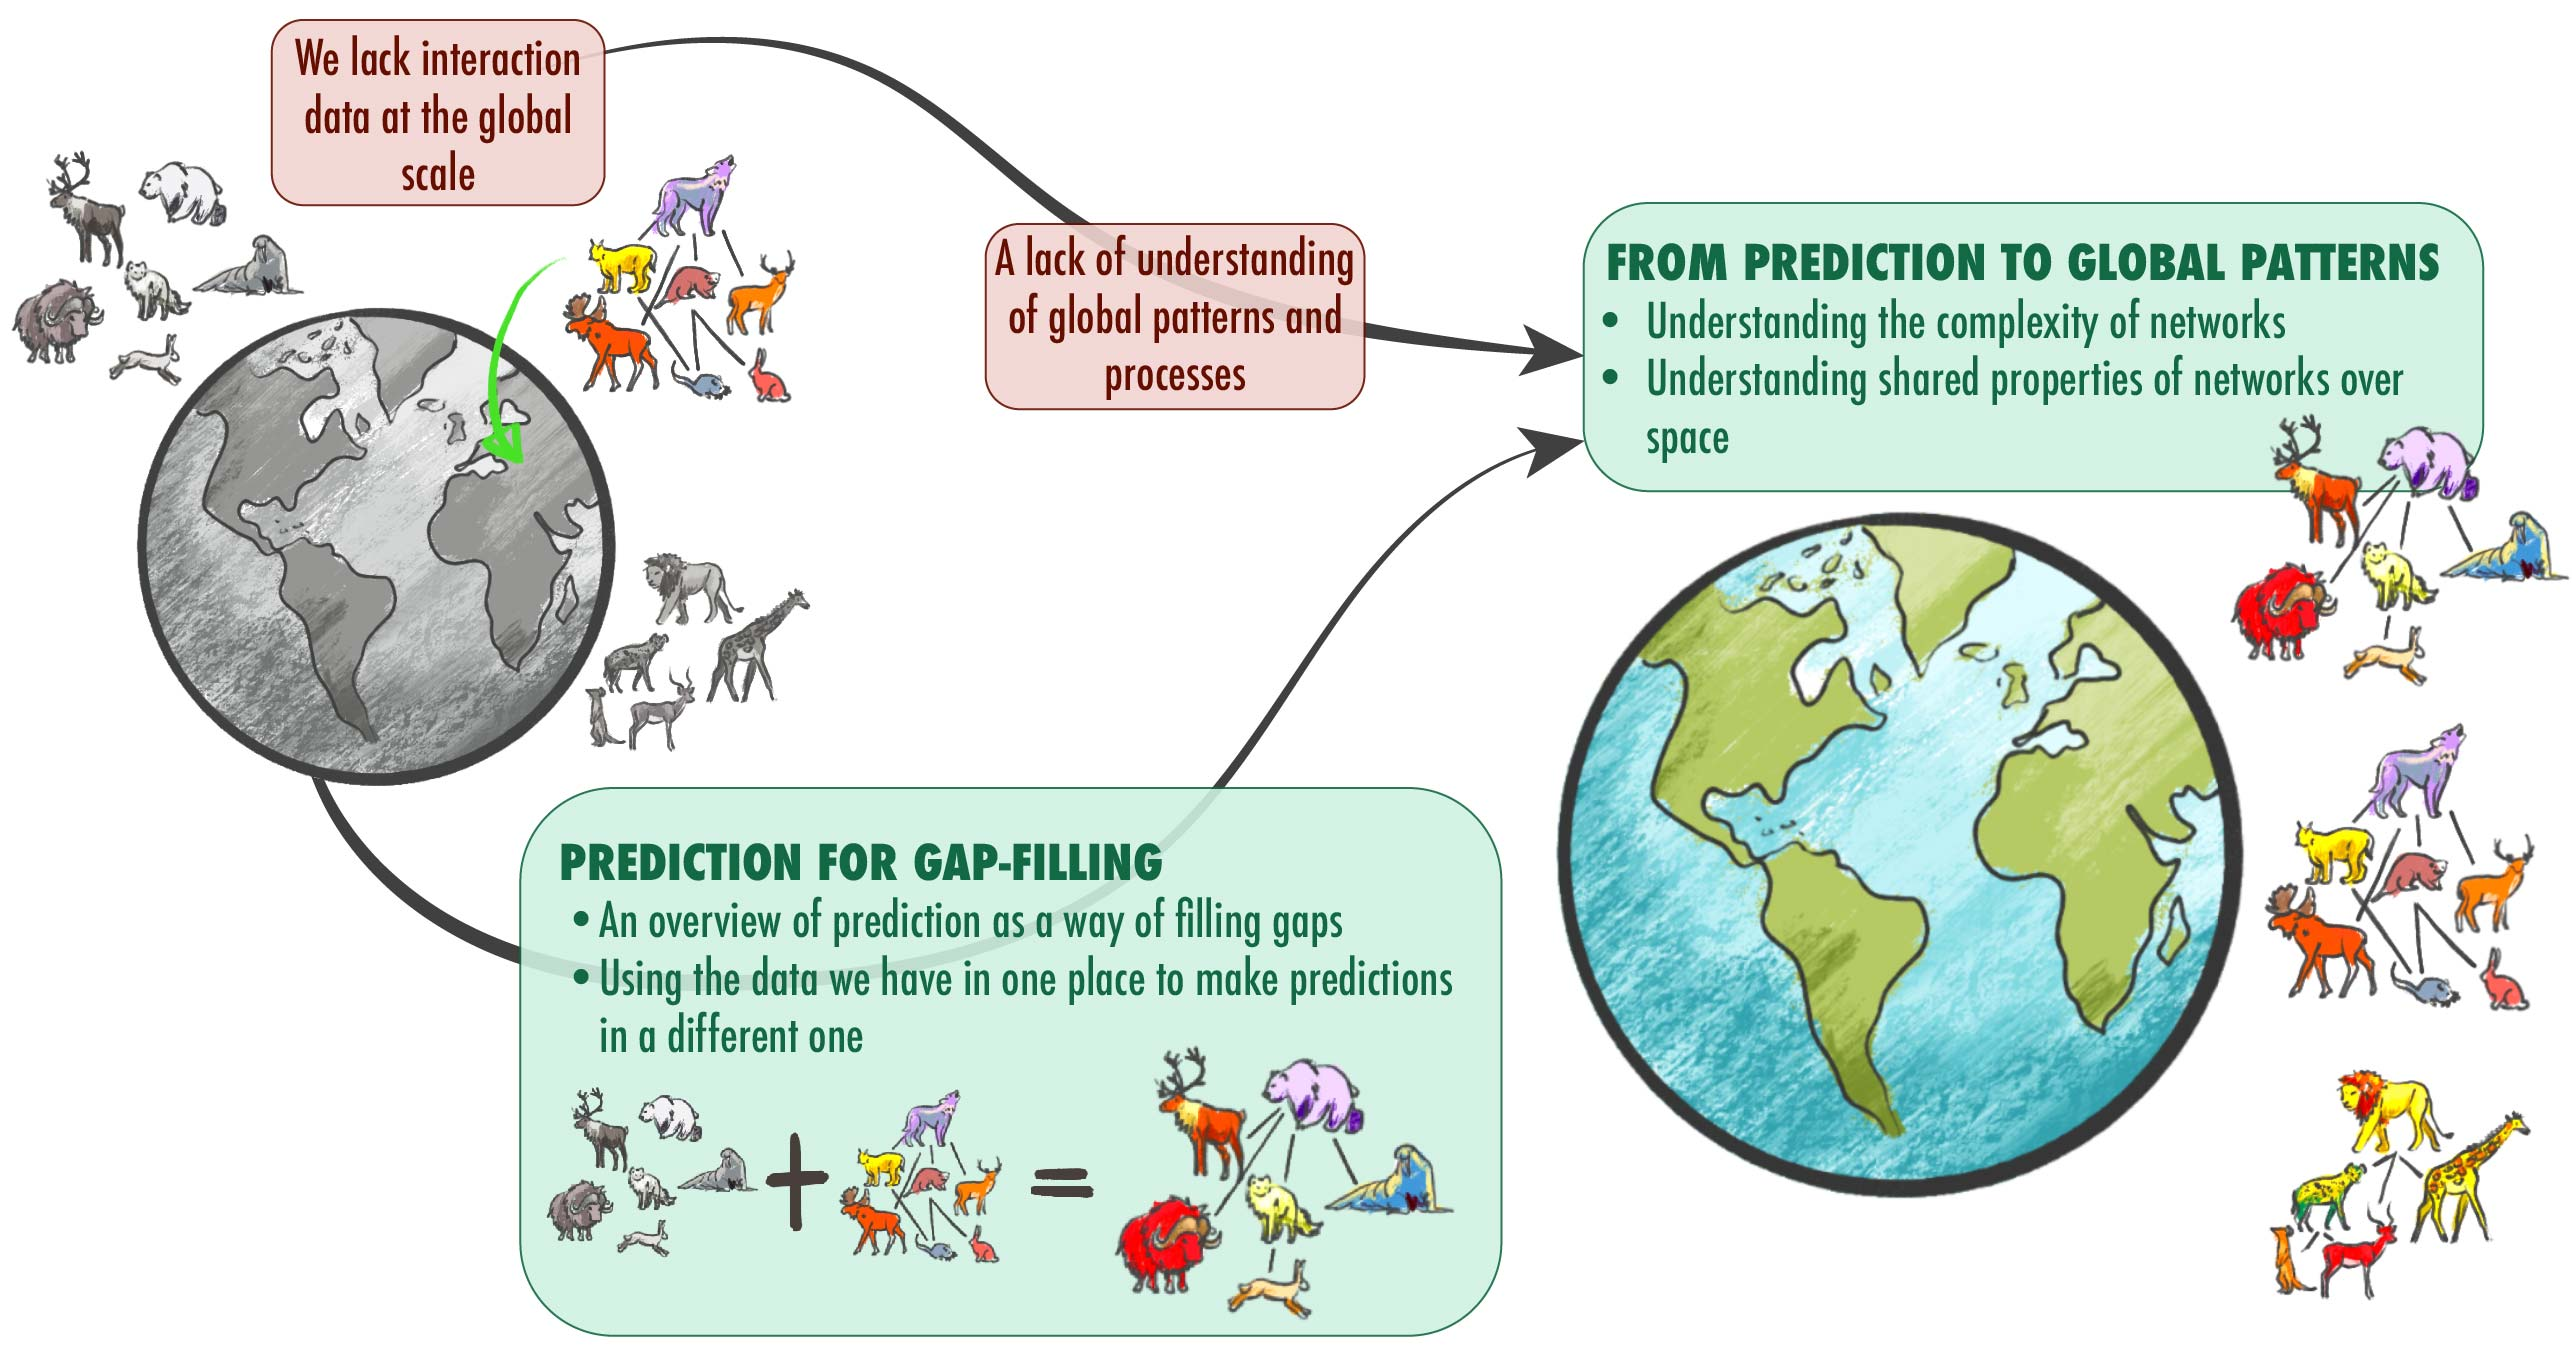
\includegraphics[width=\textwidth]{figures/thesis-flowchart.jpg}
    \caption{One of the biggest factors limiting our ability to ask global questions about ecological networks is the lack of global data. This figure provides a high-level overview of how the development and adoption of predictive methods will equip us to begin asking and answering large-scale questions.}
    \label{fig:plan}
\end{figure}

\subsection{Prediction for gap-filling}

Current methods for network prediction are often conceptualised around and focused on a single facet of species interactions, such phylogenetic matching (\cite{Pomeranz2018InfPre, Elmasri2020HieBay}), or functional traits (\cite{Bartomeus2016ComFra}). More recently applications of ensemble modelling (\cite{Becker2020PreWil}) and discussions on the potential of machine learning methods (\cite{Desjardins-Proulx2019ArtInt}) show promise in addressing methodological constraints to prediction and the growth of open tools and data may mitigate some data constraints in the coming years. However, we still lack a clear path forward or research agenda as to how we can maximise and integrate these resources to allow for ecologically plausible, and accurate, predictions.

The task of trying to predict networks is discussed in chapters \ref{Roadmap} and \ref{Perspectives}, where we map out and discuss some of the methodological considerations we are faced with when trying to approach the task of network prediction. Chapter~\ref{Roadmap} provides a more scoping discussion on these methods, whereas Chapter~\ref{Perspectives} represents a more detailed discussion on the prospect of using graph embedding and transfer learning for network prediction. These specific methods are also the framework presented and used in Chapter~\ref{Foodweb}. This section acts as a 'proof-of-concept' showcasing that the task of network prediction is both attainable and capable of producing ecologically plausible networks. Prediction is thus a way in which we can move from a scenario where we have incomplete global coverage of interaction data (\emph{i.e.,} a 'grey scaled' world) to one that exists with less gaps in the data (\emph{i.e.,} is more 'colourful'; \autoref{fig:plan}).

\subsection{From prediction to global patterns}

Although prediction is a powerful tool in the immediate/local sense 
(\emph{e.g.,} it can allow local land managers/custodians to have a 
first approximation of how species may be interacting in that given area) it is of course also a feasible way to fill in the global interaction network map. A 'filled map' will put us in the position to develop a more mechanistic, global-scaled, understanding of networks. Specifically, we need tools that will allow us to use the \emph{correct} methodology when comparing networks form different regions (\autoref{SVD}) and we can begin to leverage those data to understand the spatial structure of networks (\autoref{SpatialBoundaries}). Chapter~\ref{SVD}, which presents a different, more information theory approach to defining complexity using the singular value vector component of an SVD (\cite{Shannon1948MatThe}), and the final chapter of this thesis (\autoref{SpatialBoundaries}) is a \texttt{Julia} package that allows users to implement the Wombling algorithm (an edge detection mechanism; \cite{Womble1951DifSys}).

Ecological networks have always been deemed to be ``complex'', and an interest in the notion of complexity has (in part) been tied to network stability (\cite{Landi2018Complexity}). However the relationship between complexity and stability remains inconsistent when rigorously tested on empirical datasets (\cite{Jacquet2016NoCom}), and although ecological networks may be complex, the ways that we currently define complexity do not translate into predictions about their stability. Traditionally network ecology readily assumes that because a system has more components (\emph{e.g.,} links) it means that the system itself is complex. In \autoref{SVD} we challenge the more traditional structural (`behavioural') measures of  complexity and present SVD entropy as an alternative ('physical') measure of complexity.

Being able to subdivide networks into patches within a landscape will help us to better understand the boundaries of (and between) networks as well as how these may relate to species or community changes and boundaries - such as when transitioning across habitat `boundaries' (\cite{Hackett2019ResOur}). Wombling has been discussed as a useful tool for spatial analyses in ecology (\cite{Fortin2005SpaAna}) and has been used to detect transitions across a landscape (\cite{Philibert2008SpaStr}), changes in biological variables in communities (\cite{Barbujani1989DetReg}) and to analyse the spread of invasive species (\cite{Fitzpatrick2010EcoBou}).

\subsection{Objectives}\label{objectives-and-hypotheses}

Being able to understand, quantify, and work with ecological networks is
important from a conservation and land management perspective as this
will have cascading implications with regards to ecosystem functioning
and stability. Yet we are severely hindered by a lack of high-quality,
usable data as well as an appropriate set of tools that can be used to
contextualise and understand ecological networks. There is a need for
tools that can help us construct networks for where there are no data
\emph{i.e.,} make predictions, as well as developing tools (or ideas) that
can be used to help further our mechanistic understanding of networks once
we are at a point where we have the large scale data to do so. My work will
help address these two issues in the context of developing tools that will
either directly enable us to make predictions (Chapters~\ref{Roadmap},
\ref{Perspectives}, and \ref{Foodweb}), or present methods that are aligned
with global (large-scale) questions that will allow us to compare networks
(Chapter~\ref{SVD}) or attempt to delineate them 
(Chapter~\ref{SpatialBoundaries}).

\section{Overview of key methodological approaches}

\subsection{Transfer learning for network prediction}\label{transfer-learning-for-network-prediction}

Transfer learning is a machine learning methodology that uses the 
knowledge gained when solving a known problem and
applying it to solve a (related) problem by transferring the knowledge
across a shared medium (space; \cite{Torrey2010Transfer, Pan2010Survey}).
The concept of transfer learning is an approach that is particularly well suited for the problem of network
prediction as it allows us to lean on the data that are available to 
enable us to make \emph{de novo} interaction network predictions. This could be as simple as pinpointing missing interactions in the existing data 
(\emph{e.g.,} pairwise learning has been used to predict plant-pollinator
interactions; \cite{Stock2021Pairwise}) as well as a way to predict
novel interactions (\emph{i.e.,} fill in those global gaps) in a different location. This, in a sense, allows us to bring knowledge with us from an area for which we \emph{have} data to an area where it is \emph{lacking}. In the case of predicting species interactions, transfer learning is useful because interactions are phylogenetically conserved and thus phylogenetic relatedness can be used to predict interactions (\cite{Davies2021EcoRed, Elmasri2020HieBay, Gomez2010EcoInt}). Chapter~\ref{Foodweb} presents a transfer learning framework and uses the task of constructing a Canadian metaweb (a list of all possible interactions for a species pool) using the European metaweb assembled by (\cite{Maiorano2020Tetraeu}) as a proof-of-concept. Below is a high-level summary of that framework, and a more detailed description of the workflow can be found \href{https://osf.io/2zwqm/}{\texttt{here}}.

\subsubsection{Learning using graph embedding}\label{learning-using-embedding}

Before one can transfer any knowledge we must first learn something about the system using known interaction network. Since ecological networks can be represented by their adjacency matrices we can turn to graph theory to help us find a way to learn something about the known interaction network. Graph embedding is a low dimensional representation of the graph (interaction network) but, importantly, still preserves its topology (\cite{Yan2005Graph}). This process essentially allows us to learn something about where species (nodes) are situated within the network - which (in an abstract way) informs us of the role a species plays in the community (\emph{e.g.,} the `predator-ness' or `prey-ness' of a species). There are multiple embedding approaches discussed in Chapter~\ref{Perspectives}, but in the context of the framework developed in Chapter~\ref{Foodweb} we will focus on the use of SVD as an embedding technique. SVD presents an appropriate embedding of ecological networks, having been shown to both capture their complex, emerging properties (\cite{Strydom2021SvdEnt}) and allow for the highly accurate prediction of the interactions within a single network (\cite{Poisot2021ImpMam}).

\subsubsection{Graph embedding using SVD}

Singular Value Decomposition (\cite{Forsythe1967ComSol, Golub1971SinVal}) 
is the factorisation of an adjacency matrix \(\mathbf{A}\) (where
\(\mathbf{A}_{m,n} \in\mathbb{B}\)) into the form:

\[ \mathbf{U}\cdot\mathbf{\Sigma}\cdot\mathbf{V}^T \]

Where \(\mathbf{U}\) is an \(m \times m\) orthogonal matrix and
\(\mathbf{V}\) an \(n \times n\) orthogonal matrix. The columns in these
matrices are, respectively, the left- and right-singular vectors of
\(\mathbf{A}\). \(\mathbf{\Sigma}\) is a diagonal matrix that contains
only non-negative \(\sigma\) values.
 
An SVD can be truncated so as to remove additional noise in the dataset by
omitting non-zero and/or smaller \(\sigma\) values from
\(\mathbf{\Sigma}\) using the rank of the matrix. Under a t-SVD
\(\mathbf{A}_{m,n}\) is decomposed so that \(\mathbf{\Sigma}\) is a
square \(r \times r\) diagonal matrix (whith \(1 \le r \le r_{full}\)
where \(r_{full}\) is the full rank of \(\mathbf{A}\) and \(r\) the rank
at which we truncate the matrix). Additionally, \(\mathbf{U}_{t}\) is now a
\(m \times r\) semi unitary matrix and \(\mathbf{V}'_{t}\) an \(n \times r\)
semi-unitary matrix.

In the context of 'learning using embedding' the learned information is captured using an SVD, however for the task of network prediction we modified the products of the SVD so that they could be used for an RDPG. An RDPG  estimates the probability of observing interactions between nodes (species) as a function of the latent variables of the nodes. An RDPG allows us to turn an SVD (which consists of three matrices) into two matrices that can be multiplied to provide an approximation of the network. The latent variables used for the RDPG, called the left and right subspaces are thus constructed from an SVD and are defined as $\mathscr{L} = \mathbf{U}\sqrt{\mathbf{\Sigma}}$, and $\mathscr{R} = \sqrt{\mathbf{\Sigma}}\mathbf{V}'$ -- using the full rank of $\mathbf{A}, \mathscr{L}\mathscr{R} = \mathbf{A}$, and using any smaller rank results in $\mathscr{L}\mathscr{R} \approx \mathbf{A}$. These subspaces are ecologically informative and tell us about the 'generality' (think predator capacity, \emph{sensu} \cite{Schoener1989Food}) and  'vulnerability' (think capacity to be prey, \emph{sensu} \cite{Schoener1989Food}) of the species in the European network. This in essence provides us with an idea of where a species is likely to occur within a network/the space it occupies in the network.

\subsubsection{Transferring and inferring using phylogenetic relatedness}

In order to transfer the knowledge (the generality and vulnerability values) from a known network to the destination species pool (\emph{i.e.,} a community for which we have no interaction data), we performed ancestral character estimation using a Brownian motion model and the \cite{Upham2019Inferring} mammalian phylogeny. This uses the estimated feature vectors (left and right subspaces) for the species from the known network to create a state reconstruction for all species and allows us to impute the missing generality and vulnerability values for the destination species pool that are not already in the known network. Essentially this allows us to infer where in the two subspaces the destination species are located.

\subsubsection{Novel Prediction using RDPG}

As we now essentially have the left and right subspaces for the destination species pool we can directly multiply these to yield the metaweb, specifically using an RDPG. Because of how the phylogenetic reconstruction was implemented the left and right subspaces have an associated uncertainty, therefore, we can assemble a \emph{probabilistic} metaweb, \emph{sensu} \cite{Poisot2016Structure}, \emph{i.e.,} in which every interaction is represented as a single, independent, Bernoulli event of probability \(p\).

\subsection{SVD entropy: a measure of network
complexity}\label{svd-entropy-a-measure-of-network-complexity}

We can also use SVD as a way to define the complexity of a network. Two potential candidate measures of complexity can be derived based on the `physical structure' of (\emph{i.e.,} information within) a network. The first measure is the rank of the matrix. The rank of $\mathbf{A}$ (noted as $r = \text{rk}(\mathbf{A})$) is the dimension of the vector space spanned by the matrix and corresponds to the number of linearly independent rows or columns, which works as an estimate of its `external complexity', since it describes the dimensionality of the vector space of the matrix. Looking at this from an ecological standpoint, we can think of the this as quantifying the number of unique `strategies' within a network.

The second measure is to calculate the entropy of the matrix obtained through SVD by using the singular values \cite{Shannon1948MatThe}. This so-called SVD entropy measures the extent to which each rank encodes an equal amount of information (as the singular values capture the importance of each rank to reconstruct the original matrix) this approach therefore serves as a measure of `internal complexity'.

Intuitively, the singular value $i$ ($\sigma_i$) measures how much of the dataset is (proportionally) explained by each vector - therefore, one can measure the entropy of \(\mathbf{\sigma}\) following \cite{Shannon1948MatThe}. High values of SVD entropy reflects that all vectors are equally important, \emph{i.e.,} that the structure of the ecological network cannot be efficiently compressed, and therefore indicates a high complexity (\cite{Gu2016HowLon}). Because networks have different dimensions, we can use Pielou's evenness (\cite{Pielou1975EcoDiv}) to ensure that values are lower than unity, and quantify SVD entropy, using $s_i = \sigma_i/\text{sum}(\sigma)$ as:

$$J = -\frac{1}{\ln(k)}\sum_{i=1}^k s_i\cdot\ln(s_i)$$

Where \(k = \text{rk}(\mathbf{A})\) \emph{i.e.,} the rank of the matrix, which is equal to the number of non-zero entries in \(\mathbf{\Sigma}\) as per the Eckart-Young-Mirsky theorem (\cite{Eckart1936AppOne, Golub1987GenEck}). 

\subsection{Spatial wombling for edge detection}

Spatial wombling (an edge detection algorithm; \cite{Womble1951DifSys}). Chapter~\ref{SpatialBoundaries} presents a \texttt{Julia} package that implements both the lattice and triangulation wombling algorithms. Broadly, wombling interpolates between a given set of points but in addition to looking at the deference between said points it also looks at the direction (slope) of the difference between points. First we can calculate the rate of change \(m\) which is calculated as:

$$m = \sqrt{\frac{\partial f(x,y)}{\partial x}^2 + \frac{\partial
f(x,y)}{\partial y}^2}$$

This can be used to find the zones of rapid change across the landscape and identify potential candidate boundaries (which would be where change is occurring most rapidly). It is also possible to calculate the direction (\(\theta\)) for each rate of change. This is calculated as:

$$\theta = \arctan \left( \frac{\partial f(x,y)}{\partial y} \bigg/ \frac{\partial f(x,y)}{\partial x} \right) + \Delta$$

$$\text{where} \quad \Delta =
\left\{ \begin{array}{ccc}
    0 \degree & \text{if} & \frac{\partial f(x,y)}{\partial x} \geq 0 \\
    180 \degree & \text{if} & \frac{\partial f(x,y)}{\partial x} < 0 \\
\end{array} \right\}$$

Both $m$ and $\theta$ are an approximation on the `topology' of a certain metric ($z$, \emph{e.g.,} number of species) between a collection of points in a landscape. Similarity between the $z$ values indicates a uniformity between those points and thus a low rate of change whereas a high degree of difference between points is indicative of rapid change \emph{i.e.,} a boundary as we transition from one zone to the next.

\subsubsection{Lattice wombling}

For a lattice of points where one will have sampling locations arranged
the 'topology' \emph{i.e.} function of the landscape as determined by $z$ ($f(x,y)$) can be defined as:

$$f(x,y) = z_{1}(1-x)(1-y) + z_{2}x(1-y) + z_{3}x y + z_{4}(1-x)y$$

\subsubsection{Triangulation wombling}

When working with points that are irregularly distributed across the landscape it is possible to use triangulation wombling (\cite{Fortin1995DelEco}). The three nearest neighbours can be determined using a Delaunay triangulation algorithm \cite{Delaunay1934SphVid} and $f(x,y)$ can be defined as:

$$f(x,y) = ax + by + c$$

where:

$$ \left[ \begin{array}{ccc} a & b & c \end{array} \right] = 
\left[ {\begin{array}{ccc}
   x_{1} & y_{1} & 1\\
   x_{2} & y_{2} & 1\\
   x_{3} & y_{3} & 1\\
  \end{array} } \right]^{-1}\cdot
  \left[
  \begin{array}{ccc} z_{1} & z_{2} & z_{3} \end{array} \right]$$

and the position of the centroid between points is calculated as follows:

$$ \Big( \frac{x_{1} + x_{2} + x_{3}}{3} \Big), \Big( \frac{y_{1} + y_{2} +
y_{3}}{3} \Big) $$

\subsubsection{Boundary detection}

Detecting boundaries \emph{i.e.,} areas where the angle of the landscape
transitions sharply is surprisingly simple. After having calculated the
rate of change (\(m\)) for the geographical area it is possible to use
these values to identify and assign potential boundaries
(\cite{Fortin2005SpaAna, Oden1993CatWom, Fortin1995DelEco}). Following the
approach outlined in \cite{Fortin2005SpaAna}, a threshold value (or
percentile class) can be set and will determine what proportion of cells
will be retained as potential boundaries.

\section{Chapter summaries}

\subsection{Chapter 1: A roadmap for predicting ecological networks}

Chapter~\ref{Roadmap} maps out a series of questions and considerations with regards to approaching the challenge of predicting species interactions across space and time. This chapter represents a scoping overview of the 'gap-filling' portion of this thesis and strongly focuses on the idea of networks as predictable objects. Section~\ref{predicting-species-interaction-networks-across-space-challenges-and-opportunities} starts by outlining the challenges that might limit our ability to predict networks (which is primarily due to a limitation in data) but also looks into the opportunities we have to try and circumvent or overcome these limitations. Overall this section highlights the fact that one of the most limiting factors for prediction (a lack of data) is also the reason we need predictive tools (to overcome the lack of data), and that we are (methodologically and computationally) in a place where we can start to make feasible predictions, particularly if we think about combining different data sources.

Section~\ref{a-case-study-deep-learning-of-spatially-sparse-host-parasite-interactions} does exactly this by providing a proof-of-concept showcasing the use of co-occurrence and known interactions to predict novel interactions. This is done using the \cite{Hadfield2014TalTwo} dataset, which describes 51 host-parasite networks sampled across space. Essentially this showcases how we can extract features for each species based on co-occurrence, use said features to train an artificial neural network to predict interactions, and apply this classifier to the original features to predict potential interactions across the entire species pool. This framework essentially allows us to 'correct' any false negatives (interactions recorded as missing but are actually plausible) within the existing data. This is particularly meaningful as interactions intrinsically vary across space and time, and given the number of species that compose ecological communities, it can be tough to distinguish between a true negative (where two species never interact) from a false negative (where two species have not been observed interacting even though they actually do).

The final part of this manuscript (\autoref{a-primer-on-predicting-ecological-networks}) aims to provide a practical overview of different components to think about and take into consideration when wanting to predict networks. This body of work is intended to be something that can be taken and used as a brief primer, and as such focuses on discussing some fundamental ideas and concepts. This includes breaking down aspects of the modelling process, aspects of species interaction networks (and the interactions within them), and predicting networks over space and time. As a whole, this chapter really serves to sketch out the 'nuts and bolts' of wanting to take on the task of network prediction and serve as a useful roadmap for those wishing to find a more practical and attainable approach to addressing the global interaction data shortage.

\subsection{Chapter 2: Graph embedding for network prediction}

This chapter should be viewed as a prospective companion piece to the more 'tangible' methods presented in \autoref{Foodweb}, and is strongly rooted in the realm of thinking about network prediction. This chapter is still related to the idea of transfer learning for network prediction, however it focuses more on the expanding how we think about (and can use) a metaweb, as well as potential (alternative) graph embedding methodologies. This chapter thus pushes forward the 'we need gap-filling methods' agenda of this thesis and helps in providing a larger discussion as to the alternative ways we can modify and approach the transfer learning framework from \autoref{Foodweb}.

Section~\ref{a-metaweb-is-an-inherently-probabilistic-object} provides a discussion on how we can push the original definition of a metaweb developed by \cite{Dunne2006Network} in a new 'prediction friendly' direction. As the term 'metaweb' has been used multiple times it is perhaps useful to define it with regards to its original function -- to act as an inventory of all possible interactions for a given community. This means that as a concept a metaweb is a realistic, and attainable object to try and predict, however, it is beneficial to move away from thinking of the interactions in a metaweb as binary and rather define the interactions as Bernoulli events. Fundamentally this will allow us greater flexibility in how we weight rare interactions, provide a more nuanced overview of how the community is actually interacting, or factor in a sense of 'uncertainty' into our predictions.

Section~\ref{graph-embedding-offers-promises-for-the-inference-of-potential-interactions} provides a more detailed overview and discussion of how graph embedding works and why it is a useful way to approach network prediction. This section also includes examples of different graph embedding techniques, and (where possible) their applications to network ecology. The fundamental argument in favour of using network embedding for network prediction is that it is capturing elements of the \emph{structure} of a network (as opposed to pairwise learning of species $a$ eats $b$) and thus provides a more powerful abstraction of a network that can be used for predicting networks for other, non-related, communities. There is also an illustration of the embedding process, which is discussed in \autoref{an-illustration-of-metaweb-embedding} and acts as a way to showcase how the embedding process captures ecological processes. A more in-depth tutorial/breakdown of the analysis can be accessed through \autoref{supp:perspectives}.

The final section (\autoref{identifying-the-properties-of-the-network-to-embed}) is more focused on the limitations and scope of network embedding and prediction. There is a particular focus on the limitations of taxonomic overlap and the need for 'just the right amount' of species to be shared between known and target communities. There is of course also the challenge of political scale and how the construction of metawebs are at regional scales that may not be ecologically relevant (but are relevant for policy making). Although we are not able to confidently provide a solution for this problem (as we do not even know what an 'ecologically relevant scale' is) it is still important to think about and grapple with these topics.

\subsection{Chapter 3: Prediction in action: The Canadian Metaweb}

Building on the ideas in \autoref{Roadmap}, work on the use of 
transfer learning for predicting \emph{de novo} interactions
(\cite{Runghen2021Exploiting}), and the applicability of phylogenetic
reconstruction within the context of ecological networks \emph{e.g.,}
(\cite{Braga2021Phylogenetic}), we set out to create a probabilistic metaweb for
terrestrial Canadian mammals in \autoref{Foodweb}. Despite their importance in many ecological processes, collecting data and information on ecological interactions is an exceedingly challenging task. For this reason, large parts of the world have a data deficit when it comes to species interactions and how the resulting networks are structured. A key premise of this chapter is the idea of being able to take the information that we do have and bring it with us to predict networks in an area where we have no information. This is fundamentally a chance to 'put our money where our mouth is' and provide a \emph{tangible} way to approach (and round out) the gap-filling portion of this thesis. Specifically, this framework allows us to ‘learn’ the information (latent traits) of species from a known interaction network (in this case, the European metaweb) and infer the latent traits of another species pool for which we have no \emph{a priori} interaction data (in this case Canadian species) based on their phylogenetic relatedness to species from the known network (see section~\ref{transfer-learning-for-network-prediction} for a more detailed summary of the methodology). 

Using the prediction of the Canadian metaweb as a way to test the methodology presented in this chapter is useful as we have existing datasets with which to test the validity of our predictions. What is perhaps most exciting about this chapter is that despite sharing about only 4\% of species between Canada and Europe we were able to construct a metaweb that correctly predicted about 91\% of the species interactions in Canada. It should also be noted that when comparing  the European and Canadian metawebs we see a difference in their structures (\autoref{rdpg-reconstructed-networks-have-diverse-structures}), implying that the embedding process is not 'copy pasting' the European network and filling in Canadian species but rather capturing an ecological process.

In addition to testing the validity of the predicted interactions within the Canadian metaweb we also did some additional tests using just the European metaweb. In this instance interactions within the European network were modified (either removed or new interactions were added) and the modified network was used to predict a 'new' European network. This allowed us to compare how well the model could recover the original network despite being 'given' erroneous information. Overall the model is robust to both the addition as well as removal of interactions, although the removal of interactions does have a more negative effect on the ability of the model to recover interactions (\autoref{rdpg-yields-an-accurate-classifier})

Overall it appears that the transfer learning framework presented in this chapter is quite robust and has potential applicability in a variety of settings (\emph{e.g.,} generating metawebs that can be used as `informative priors' from which more localised/spatially explicit networks can be constructed, \cite{Cirtwill2019QuaFra}), can be given to a local expert for more refined validation, and overall presents a potential mechanism to begin filling in the global gaps.

\subsection{Chapter 4: SVD entropy: a measure of network complexity}

In \autoref{SVD} we present SVD entropy as a starting point to
unifying (and standardising) how we define the complexity of ecological
networks. In the perspective of 'global questions about patterns' this of course presents a way in which we can ask a simple question - do different networks (in the case of this chapter different bipartite networks) have differences in their complexity. What makes SVD entropy a compelling metric for quantifying complexity (when comparing to the more 'standard', structural measures such as nestedness, connectance, and spectral radius) is that it focuses more on the 'physical' complexity of the network as opposed to the complexity of the behaviour of the system. This is because the structural measures of complexity are capturing an emerging property of the network, whereas SVD entropy captures the information contained in the the network (one can think of this as the 'compressibility' of the network, more complex networks are harder to compress).

The primary take away from this chapter is that (at least bipartite networks) are exceptionally complex. In \autoref{most-ecological-networks-are-close-to-full-rank} we can see that networks have a relative rank deficiency of zero (\emph{i.e.,} they have a maximal 'external complexity') and all networks have an SVD entropy value greater than 0.80, \emph{i.e.,} near maximal 'internal complexity' (for context the way that SVD entropy is calculated means that values are constrained between zero and one). In \autoref{most-elements-of-network-structure-capture-network-complexity} we also looked at the corresponding connectance, nestedness, and spectral radius of these networks . Although there is a correlation between the calculated entropy and these other metrics the story that is told by the different metrics is different. Namely, for the structural metrics the 'complexity' spans the entire potential range of of values, and there is the potential for 'misinterpreting' what could be considered complex. For example networks that have a maximal nestedness have the lowest SVD entropy (\emph{i.e.,} the lowest physical complexity), this is not necessarily the most intuitive way to interpret a maximal nestedness. This 'breakdown' of what complexity means is also echoed in \autoref{complex-networks-are-not-more-robust-to-extinction}, here we simulated extinctions to get a measure of network resilience (since a common adage is that complexity begets stability), however we do not see a strong relationship between SVD entropy and resilience. This again highlights that 'structural' and 'physical' complexity metrics are capturing different facets of a network, and although it is not to say that SVD entropy is a 'better' way to measure the complexity of a network it does highlight that we need to be mindful of how we are defining 'complexity' and particularly how that might impact on how we interpret results based on the complexity of networks.

An additional interesting result discussed in \autoref{larger-networks-are-less-complex-than-they-could-be} is that although the complexity of ecological networks is indeed \emph{immense} they are still not reaching their \emph{maximum} potential complexity, which implies that \emph{something} might be constraining network complexity. This result is echoed in \autoref{connectance-constrains-complexity-but-also-rank-deficiency}, which looks at the relationship between network size, connectance and complexity. Results point to the potential constraint of network size on complexity. One possible explanation is that networks at the early assembly stages tend to be severely constrained (\cite{Barbier2018GenAss, Saravia2018EcoNet}) due to conditions needed for the persistence of multiple species. As networks grow larger, these constraints may ``relax'', leading to networks with more redundancy, and therefore a lower complexity.

\subsection{Chapter 5: SpatialBoundaries.jl: a software for boundary detection}

In this chapter we present a \texttt{Julia} package \texttt{SpatialBoundaries.jl}, (the documentation is available \href{https://poisotlab.github.io/SpatialBoundaries.jl/dev/}{here}) that has the functionality to implement the spatial wombling algorithm across both a uniform landscape \emph{i.e.,} lattice wombling as well as irregular/random landscapes \emph{i.e.,} triangulation wombling. These two methods still calculate the rate of change (\(m\)) and directionality (\(\theta\)) in the same manner but differ in how the aggregate and quantify the surface for a set of points (\cite{Fortin2005SpaAna}). These two algorithms provide functionality for most use cases when data are quantitative. \texttt{SpatialBoundaries.jl} has also been developed so as to integrate with other packages such as \texttt{SimpleSDMLayers.jl}.

Overall this chapter is 'simple' in its content (a software package that can implement the spatial wombling algorithm) however it has been developed with the forward-scoping idea of being used within the context of thinking about boundaries between networks (or if they are even present) and thus aligns well with the idea of developing tools for understanding global/large scale network patterns. Some ideas for implementing this package are presented in \autoref{supp:boundaries}, and primarily rest on the idea of using a combination of a metacommunity model and simulated landscapes to see if networks, species, and environmental boundaries show a high degree of fidelity or not. The work presented in \autoref{supp:boundaries} should be treated as a speculative outline of what we can do with the \texttt{SpatialBoundaries.jl} in the context of network analysis and could be viewed as an rough first draft on trying to understand 'where networks stop?', which echoes one of the challenges discussed in \autoref{Perspectives}, particularly in \autoref{identifying-the-scope-of-the-prediction-to-perform}.

\section{Conclusion}\label{conclusion}

As a whole this thesis should be viewed as a computational toolbox for
network ecology that addresses both the issue of data scarcity through
the use of predictive tools (addressing the `Eltonian shortfall' highlighted by \cite{Hortal2015Seven}) as well as presenting methods/ideas geared towards thinking about networks at global scales. This means that we would \emph{i}) have `tangible' networks from which we can begin to work with in various contexts or situations and \emph{ii}) have new methods/tools to begin asking questions about networks at a global scale. In other words adding more building blocks from which we can begin to take network ecology to the next level, \emph{i.e.,} bridging the gap from 'local-level network understanding' to 'tools for global network analysis'.

\printbibliography{}
\end{refsection}

\endinput
%%
%% End of file `introduction.tex'.


%%%%%%%%%%%%%%%%%%%%%%%%%%%%%%%%%%%%%%%%%%%%%%%%%%%%%%%%%%%%
%%%%%%%%%%%%%%%%%%%%                   %%%%%%%%%%%%%%%%%%%%%
%%%%%%%%%%%%%%%%%%%%  A R T I C L E S  %%%%%%%%%%%%%%%%%%%%%
%%%%%%%%%%%%%%%%%%%%                   %%%%%%%%%%%%%%%%%%%%%
%%%%%%%%%%%%%%%%%%%%%%%%%%%%%%%%%%%%%%%%%%%%%%%%%%%%%%%%%%%%

%%
%% This is file `article1.tex',
%% generated with the docstrip utility.
%%
%% The original source files were:
%%
%% dms.dtx  (with options: `article')
%% Example TeX file for the documentation
%% of the jurabib package
%% Copyright (C) 1999, 2000, 2001 Jens Berger
%% See dms.ins  for the copyright details.
%% 
%%% ====================================================================
%%%  @LaTeX-file{
%%%     filename        = "dms.dtx",
%%%     author    = "Nicolas Beauchemin, Damien Rioux-Lavoie, Victor Fardel, Jonathan Godin",
%%%     copyright = "Copyright (C) 2000 , DMS
%%%                  all rights reserved.  Copying of this file is
%%%                  authorized only if either:
%%%                  (1) you make absolutely no changes to your copy,
%%%                  including name; OR
%%%                  (2) if you do make changes, you first rename it
%%%                  to some other name.",
%%%     address   = "Département de Mathématiques et de Statistique",
%%%     telephone = "514-343-6705",
%%%     FAX       = "514-343-5700",
%%%     email     = "aide@dms.umontreal.ca (Internet)",
%%%     keywords  = "latex, amslatex, ams-latex, theorem",
%%%     abstract  = " Ce fichier est un package conçu pour être
%%%                  utilisé avec la version de LaTeX2e 1995/06/01. Il
%%%                  est prévue pour la classe ``amsbook''. Il en
%%%                  modifie le format des pages, l'entête des
%%%                  sections, etc, afin d'être  conforme au modèle de
%%%                  mémoire de maîtrise de l'Université de
%%%                  Montréal. Finalement ce fichier est grandement
%%%                  inspiré du fichier amsclass.dtx.",
%%%     docstring = "The checksum field contains: CRC-16 checksum,
%%%                  word count, line count, and character count, as
%%%                  produced by Robert Solovay's checksum utility."}
%%%  ====================================================================


%% To change chapter header dynamically from french to english, use
%%\entetedynamique
\setcounter{corA}{0} % Pour recommancer à compter les def,
                     % theo, etc. à partir de 1
 % Pour écrire un article en français
%%\francais
 % Pour écrire un article en anglais
\anglais
%% NOTE: La plupart des macros ont un nom en anglais.
%% P.ex. \adresse et \address fonctionnent et sont équivalents.
%% \revue=\journal
%% \auteur=\author
%% \titre=\title

\doublespacing

%% Les contributions apparaîtront habituellement après
%% \maketitle (voir un peu plus bas). Selon les goûts, il est
%% possible de mettre les contributions
%% avant la page titre de l'article, simplement en les écrivant
%% directement ici. Par exemple :
 % \cleardoublepage
 % \pdfbookmark[chapter]{Contributions}{contrib1} % Remplacer par contrib2 pour l'article 2 etc.
 % {\bfseries\Large\noindent Contributions de <mon nom> et rôle joué par les coauteurs}
 % J'ai contribué en...
 %
 % Le rôle des coauteurs a été de...

%% Nom de la revue de publication
\revue{Philosophical Transactions of the Royal Society B, and can be accessed at https://doi.org/10.1098/rstb.2021.0063}
\article{A roadmap towards predicting species interaction networks (across space and time)}\label{Roadmap}
%% On peut se référer aux numéros de chapitre ou d'article comme suit.
%% Si on fait
%% \label{chap:article1},
%% alors \ref{chap:article1} donnera le numéro du chapitre. On peut ensuite faire
%% \labelart{art:article1}
%% et alors \ref{art:article1} donnera le numéro d'article.
%% Par exemple, si cette article est le premier article et le deuxième chapitre,
%% alors si on écrit
%% Voir le chapitre~\ref{chap:article1} (l'article~\ref{art:article1}).
%% deviendra
%% Voir le chapitre 2 (l'article 1).
%% Si on veut écrire « premier article » au lieu « article 1 », on peut
%% simplement faire
%% \ordinal{\ref{art:article1}}~article  % devient première article
%% ou
%% \Ordinal{\ref{art:article1}}~article  % devient Première article (avec la majuscule)
%% Si on est en mode \anglais, \ordinal écrire first, second,...

%%%%%%%%%%%%%%%%%%%%%%%%%%%%%%%%%%%%%%%%%%%%%%%%%%%%%%%%%%%%%%%
%%%%%%%%%%%%%%%%%     Contribution     %%%%%%%%%%%%%%%%%%%%%%%%
%%%%%%%%%%%%%%%%% (lire attentivement) %%%%%%%%%%%%%%%%%%%%%%%%
%%%%%%%%%%%%%%%%%%%%%%%%%%%%%%%%%%%%%%%%%%%%%%%%%%%%%%%%%%%%%%%
 % Contribution(s) peronnelle(s) à l'article et rôle joué par tous les coauteur·e·s
 %
 % Nécessaire seulement lorsque vous n'êtes pas seul·e auteur·e.
 % Les contributions peuvent apparaître ailleur dans la thèse.
 % Si \contributions est laissé vide (p.ex. si vous effacez
 % celui ci-bas), aucune contributions ne seront générées sur
 % la page titre de l'article. Vous pouvez alors mettre un
 % \newpage si vous souhaitez que les résumé et abstract soient
 % sur la page suivante.
 %
 % REMARQUE : À peu près toutes les constructions \LaTeX\ sont permises
 % dans les contributions.
 %
 % La commande admet une option [<entête>]
\contributions%[Mes contributions et le rôle des coauteurs]
{
All authors contributed to the drafting, writing and editing of the manuscript. \\[1cm]
}

%%% INFORMATIONS POUR LA PAGE TITRE
 % Premier auteur·e et adresse
\auteur{Tanya Strydom}
\adresse{Département de Sciences Biologiques, Université de Montréal, Montreal, QC, Canada\\ Québec Centre for Biodiversity Sciences, Montreal, QC, Canada}
\auteur{Michael D. Catchen}
\adresse{McGill University, Montréal, Canada\\ Québec Centre for Biodiversity Sciences, Montreal, QC, Canada}
\auteur{Francis Banville}
\adresse{Département de Sciences Biologiques, Université de Montréal, Montreal, QC, Canada\\
Université de Sherbrooke, Sherbrooke, Canada\\
Québec Centre for Biodiversity Sciences, Montreal, QC, Canada}
\auteur{Dominique Caron}
\adresse{McGill University, Montréal, Canada\\ Québec Centre for Biodiversity Sciences, Montreal, QC, Canada}
\auteur{Gabriel Dansereau}
\adresse{Département de Sciences Biologiques, Université de Montréal, Montreal, QC, Canada\\ Québec Centre for Biodiversity Sciences, Montreal, QC, Canada}
\auteur{Philippe Desjardins-Proulx}
\adresse{Département de Sciences Biologiques, Université de Montréal, Montreal, QC, Canada\\ Québec Centre for Biodiversity Sciences, Montreal, QC, Canada}
\auteur{Norma R. Forero-Muñoz}
\adresse{Département de Sciences Biologiques, Université de Montréal, Montreal, QC, Canada\\ Québec Centre for Biodiversity Sciences, Montreal, QC, Canada}
\auteur{Gracielle Higino}
\adresse{Universidade Federal de Goiás, Goiâna, Brasil}
\auteur{Benjamin Mercier}
\adresse{Université de Sherbrooke, Sherbrooke, Canada\\
Québec Centre for Biodiversity Sciences, Montreal, QC, Canada}
\auteur{Andrew Gonzalez}
\adresse{McGill University, Montréal, Canada\\ Québec Centre for Biodiversity Sciences, Montreal, QC, Canada}
\auteur{Dominique Gravel}
\adresse{Université de Sherbrooke, Sherbrooke, Canada\\
Québec Centre for Biodiversity Sciences, Montreal, QC, Canada}
\auteur{Laura Pollock}
\adresse{McGill University, Montréal, Canada\\ Québec Centre for Biodiversity Sciences, Montreal, QC, Canada}
\auteur{Timothée Poisot}
\adresse{Département de Sciences Biologiques, Université de Montréal, Montreal, QC, Canada\\ Québec Centre for Biodiversity Sciences, Montreal, QC, Canada}
%%
%% et ainsi de suite pour les autres auteurs

\maketitle

\begin{resume}{réseaux écologiques, apprentissage automatique, apprentissage profond, prévisions écologiques, biogéographie}
  Les réseaux d’interactions entre espèces sous-tendent de nombreux processus écosystémiques, mais il est difficile d’échantillonner de manière exhaustive ces interactions. Les interactions varient intrinsèquement dans l'espace et dans le temps, et étant donné le nombre d'espèces qui composent les communautés écologiques, il peut être difficile de distinguer un vrai négatif (dans lequel deux espèces n'interagissent jamais) d'un faux négatif (dans lequel deux espèces n'ont même pas été observées en interaction). bien qu'ils le fassent réellement). Évaluer la probabilité d’interactions entre espèces est un impératif pour plusieurs domaines de l’écologie. Cela signifie que pour prédire les interactions entre les espèces – et pour décrire la structure, la variation et l’évolution des réseaux écologiques qu’elles forment – nous devons nous appuyer sur des outils de modélisation. Nous fournissons ici une preuve de concept, dans laquelle nous montrons comment un simple modèle de réseau neuronal fait des prédictions précises sur les interactions entre espèces avec des données limitées. Nous évaluons ensuite les défis et les opportunités associés à l’amélioration des prédictions d’interaction et fournissons une feuille de route conceptuelle vers des modèles prédictifs de réseaux écologiques explicitement spatiaux et temporels. Nous concluons par une brève introduction aux méthodes et outils pertinents nécessaires pour commencer à construire ces modèles, qui, nous l’espérons, guideront ce programme de recherche.
\end{resume}

\begin{abstract}{ecological networks, machine learning, deep learning, ecological forecasting, biogeography}
  Networks of species interactions underpin numerous ecosystem processes, but comprehensively sampling these interactions is difficult. Interactions intrinsically vary across space and time, and given the number of species that compose ecological communities, it can be tough to distinguish between a true negative (where two species never interact) from a false negative (where two species have not been observed interacting even though they actually do). Assessing the likelihood of interactions between species is an imperative for several fields of ecology. This means that to predict interactions between species—and to describe the structure, variation, and change of the ecological networks they form—we need to rely on modelling tools. Here, we provide a proof-of-concept, where we show how a simple neural network model makes accurate predictions about species interactions given limited data. We then assess the challenges and opportunities associated with improving interaction predictions, and provide a conceptual roadmap forward towards predictive models of ecological networks that is explicitly spatial and temporal. We conclude with a brief primer on the relevant methods and tools needed to start building these models, which we hope will guide this research programme forward.
\end{abstract}

\section{Introduction}\label{introduction}

Ecosystems are, in large part, constructed by the interactions within
them --- organisms interact with one-another and with their environment,
either directly or indirectly. Interactions between individuals,
populations, and species create networks of interactions that drive
ecological and evolutionary dynamics and maintain the coexistence,
diversity, and functioning of ecosystems \cite{Delmas2018AnaEco,
Landi2018ComSta, Albrecht2018PlaAni}. Species interaction networks
underpin our understanding of numerous ecological processes
\cite{Pascual2006EcoNet, Heleno2014EcoNet}. Yet, even basic knowledge
of species interactions (like being able to list them, or guess which
ones may exist) remains one of the most severe biodiversity shortfalls
\cite{Hortal2015SevSho}, in large part due to the tedious,
time-consuming, and expensive process of collecting species interaction
data. Comprehensively sampling every possible interaction is not
feasible given the sheer number of species on Earth, and the data we can
collect about interactions tend to be biased and noisy
\cite{deAguiar2019RevBia}. This is then compounded as species
interactions are typically measured as a binary variable (present or
absent) even though it is evident interactions are not all-or-nothing.
Empirically we know species interactions occur probabilistically due to
variation in species abundances in space and time
\cite{Poisot2015SpeWhy}. Different types of interactions vary in their
intrinsic predictability (e.g.~some fungal species engage in
opportunistic saprotrophy \cite{Smith2017GroEvi}, obligate parasites are
more deterministic in their interactions than facultative parasites
\cite{Poisot2013FacObl, Luong2019FacPar}). In addition to this variance
in predictability, networks from different systems are structured by
different mechanisms.

Still, like all of Earth's systems, species interaction networks have
entered their ``long now'' \cite{Carpenter2002EcoFut}, where
anthropogenic change will have long-term, low-predictability
consequences \cite{Burkle2013PlaInt} for our planet's ecology.
Therefore, our field needs a roadmap towards models that enable
prediction (for the present) and forecasting (for the future) of species
interactions and the networks they form, and which accounts for their
spatial and temporal variation \cite{McCann2007ProBio, Seibold2018NecMul}. 
As an example, in disease ecology, predicting
potential hosts of novel disease (recently notably the search for
wildlife hosts of betacoronaviruses; \cite{Becker2020PreWil,
Wardeh2021PreMam}) has received much attention. Network approaches
have been used for the prediction of risk and dynamics of dengue
\cite{Zhao2020MacLea}, Chagas disease \cite{Rengifo-Correa2017UndTra},
Rickettsiosis \cite{Morand2020DisEco}, Leishmaniasis
\cite{Stephens2009UsiBio}, and a myriad infectious diseases in livestock
and wildlife \cite{Craft2015InfDis}. Additionally, prediction of
interaction networks is a growing imperative for next-generation
biodiversity monitoring, requiring a conceptual framework and a flexible
set of tools to predict interactions that is explicitly spatial and
temporal in perspective \cite{Edwards2021TroLan, Magioli2021DefLea,
Zhang2021PlaBre}. Developing better models for prediction of these
interactions will rely on integration of data from many sources, and the
sources for this data may differ depending on the type of interaction we
wish to predict \cite{Gibb2021DatPro}.

Interactions between species can be conceptualised in a multitude of
ways (mutualistic vs.~antagonistic, strong vs.~weak, symmetric
vs.~asymmetric, direct vs.~indirect) \cite{Jordano2016ChaEco,
Morales-Castilla2015InfBio}. What is common among definitions of
species interactions is that \emph{at least} one of the species is
affected by the presence of another \cite{Morales-Castilla2015InfBio}.
Networks can be used to represent a variety of interaction types,
including: \emph{unipartite networks}: where each species can be linked
to other species (often food webs), \emph{bipartite networks}: where
there are two pools of species and all interactions occur between
species in each pool (typically used for pairwise interactions;
e.g.~hosts and parasites), and \emph{k-partite networks,}: which expand
to more than two discrete sets of interacting species (e.g., some
parasitoid webs, seed dispersal networks, and pollination networks
\cite{Pocock2012RobRes}).

Methods for predicting interactions between species exist, but at the
moment are difficult to generalise as they are typically based around a
single mechanism at a single scale: position in the trophic niche
\cite{Gravel2013InfFoo, Petchey2008SizFor}, phylogenetic distance
\cite{Pomeranz2018InfPre, Elmasri2020HieBay}, functional trait matching
\cite{Bartomeus2016ComFra}, interaction frequency
\cite{Weinstein2017ComTra, Vazquez2005IntFre}, or other network
properties \cite{Terry2020FinMis, Stock2017LinFil}. Species interaction
networks, as we observe them on Earth today, are the product of
ecological and evolutionary mechanisms interacting across spatial,
temporal and organisational scales. The interwoven nature of these
processes imposes structure on biodiversity data which is invisible when
examined only through the lens of a single scale, however machine
learning (ML) methods have enormous potential to find this structure in
data \cite{Desjardins-Proulx2019ArtInt}, and have the potential to be
used together with mechanistic models in order to make prediction of
ecological dynamics more robust \cite{Rackauckas2020UniDif}.

Here we use a case study to show how machine-learning models
(specifically a deep neural network) can enable prediction of species
interactions: we construct a metaweb of host-parasite interactions
across space, using predictors extracted from empirical data and
accounting for the structure of co-occurrence between species. We use
this case study to illustrate a roadmap for improving predictions using
open data and ML methods; specifically, we focus on how emerging tools
from ML can be used to deliver more accurate and more efficient
predictions of ecological systems, and how the potential of these
approaches will be magnified with increased data access. We then provide
a non-exhaustive primer on the literature on interaction prediction, and
identify the tools and methods most suited for the future of interaction
network prediction models, covering the spatial, temporal, and climatic
dimensions of network prediction \cite{Burkle2011FutPla}. Both the case
study and primer are largely geared towards binary (interactions are
either present or absent) networks; there are limitations in data and
tools that make it a more reasonable starting approach. First, most
ecological networks do not have estimates of interaction strength, and
particularly not estimates that are independent from relative
abundances. Second, the methodological toolkit to analyse the structure
of networks is far more developed for binary interactions
\cite{Delmas2018AnaEco}, meaning that the predictions of binary
interactions can be more readily interpreted.

We argue that adopting a more predictive approach to complex ecological
systems (like networks) will establish a positive feedback loop with our
understanding of these systems \cite{Houlahan2017PriPre}: the tasks of
understanding and predicting are neither separate nor opposed
\cite{Maris2017PreEco}; instead, ML tools have the ability to capture a
lot of our understanding into working assumptions, and comparing
predictions to empirical data gives us better insights about how much we
ignore about the systems we model (see for example
\cite{Borowiec2021DeeLea}, who provide an overview of deep learning techniques
and concepts in ecology and evolution). Although data on species
interaction networks are currently limited in the size and spatial
coverage, machine learning approaches have a demonstrated track record
of revealing the ``unreasonable effectiveness'' of data
\cite{Halevy2009UnrEff}; we argue that with a clear roadmap guiding the
use of these methods, the task of predicting species interaction
networks will become more attainable.

\section{A case study: deep learning of spatially sparse host-parasite
interactions}\label{a-case-study-deep-learning-of-spatially-sparse-host-parasite-interactions}

The premise of this manuscript is that we can predict interactions
between species. In this section we provide a proof-of-concept, where we
use data from \cite{Hadfield2014TalTwo} describing 51 host-parasite networks
sampled across space. In this data, as in most spatially distributed
ecological networks, not all species co-occur across sites. As a direct
consequence there are pairs of species that may or may not be able to
interact for which we have no data; furthermore there are pairs of
species that may interact, but have only been documented in a single
location where the interaction was not detected. In short, there are
ecological reasons to believe that a number of negative associations in
the metaweb (\emph{sensu} \cite{Dunne2006NetStr}) are false negatives.

Without any species-level information, we resort to using both
co-occurrence and known interactions to predict novel interactions. To
do this we (i) extract features (equivalent to explanatory variables in
a statistical model) for each species based on co-occurrence, (ii) use
these features to train an artificial neural network to predict
interactions, and (iii) apply this classifier (an algorithm that assigns
a categorical output based on input features) to the original features
to predict potential interactions across the entire species pool.
Machine learning relies on a lexicon that shares some terms with
statistics, albeit with different meaning; we expand on the precise
meanings in the ``How to validate a predictive model'' section below.
The outputs of the analysis are presented in \autoref{fig:example}, and the code
to reproduce it is available at \texttt{https://osf.io/6jp4b/}; the
entire example was carried out in \texttt{Julia 1.6.2}
\cite{Bezanson2017JulFre}, using the \emph{Flux} machine learning
framework \cite{Innes2018FluEle}.

We first aggregate all species into a co-occurrence matrix \(A\) which
represents whether a given pair of species \((i,j)\) was observed
coexisting across any location. We then transform this co-occurrence
matrix \(A\) via probabilistic PCA \cite{Tipping1999ProPri} and use the
first 15 values from this PCA space as the features vector for each
species \(i\). For each pair of (host, parasite) species \((i,j)\), we
then feed the features vectors \((v_i, v_j)\) into a neural network. The
neural network uses four feed-forward layers (each layer is independent
from the one before and after); the first layer uses the \(\text{RELU}\)
activation function (which ignores input below a threshold), the rest
use a \(\sigma\) function (which transforms linear activation energies
into logistic responses). All layers have appropriate dropout rates (in
order to avoid over-fitting, only a fraction of the network is updated
on each iteration: \(1-0.8\) for the first layer, \(1-0.6\) for the
subsequent ones). This produces an output layer with a single node,
which is the probability-score for interaction between species \(i\) and
\(j\).

We then train (equivalent to \emph{fit}) this neural network by dividing
the original dataset into testing and training sets (split 80-20 for
training and testing respectively). During the training of this neural
network (using the ADAM optimiser), the \(5\times 10^4\) batches of 64
items used for training were constrained to have at least 25\% of
positive interactions, as \cite{Poisot2021ImpMam} show slightly inflating the
dataset with positive interactions enables us to counterbalance sampling
biases. Furthermore, setting a minimum threshold of response balance is
an established approach for datasets with strong biases
\cite{Lemaitre2017ImbPyt}. Validating this model on the test data shows
our model provides highly effective prediction of interactions between
pairs of species not present in the training data (Fig.\ref{fig:example}). The
behaviour of the model was, in addition, checked by measuring the
training and testing loss (difference between the actual value and the
prediction, here using mean-squared error) and stopping well before they
diverged (to avoid overfitting).

\begin{figure}[h]
    \centering
    \includegraphics[width=\textwidth]{figures/figure1.png}
    \caption{Proof-of-Concept: An empirical metaweb (from
\cite{Hadfield2014TalTwo}, i.e.~a list of known possible interactions
within a species pool, is converted into latent features using
probabilistic PCA, then used to train a deep neural network to predict
species interactions. Panels A and B represent, respectively, the ROC
curve and the precision-recall curve, with the best classifier
(according to Youden's J) represented by a black dot. The expected
performance of a neutral ``random-guessing'' classifier is shown with a
dashed line. Panel C shows the imputed using t-distributed stochastic
neighbour embedding (tSNE), and the colours of nodes are the cluster to
which they are assigned based on a \(k\)-means clustering of the tSNE
output. Empirical interactions are shown in purple, and imputed
interactions in grey.}
    \label{fig:example}
\end{figure}

This case study shows that a simple neural network can be very effective
in predicting species interactions even without additional species-level
data. Applying this model to the entire dataset (including species pairs
never observed to co-occur) identified 1546 new possible interactions --
746 (48\%) of which were between pairs of species for which no
co-occurrence was observed in the original dataset. This model reaches
similar levels of predictive efficacy as previous studies that use far
more species-level data and mechanistic assumptions
\cite{Gravel2013InfFoo}, which serves to highlight the potential for
including external sources of data for \emph{improving} our prediction
of interaction networks even further. For example, \cite{Krasnov2016TraPhy}
collected traits data for this system that could be added to the model,
in addition or in substitution to latent variables derived from observed
interactions.

\section{Predicting species interaction networks across space:
challenges and
opportunities}\label{predicting-species-interaction-networks-across-space-challenges-and-opportunities}

Here we present a conceptual roadmap (\autoref{fig:conceptual}) which shows a
conceptual path from data to prediction of species interaction networks,
incorporating several modelling frameworks. We envisage this roadmap to
be one conceptual path toward incorporating space in to our prediction
of interaction networks, and developing spatially explicit models of
networks and their properties. In the following sections we discuss the
challenges and opportunities for this path forward, and highlight two
specific areas where it can have a strong impact: the temporal
forecasting of species interaction networks structure, and the use of
predicted networks for applied ecology and conservation biology.

\begin{figure}[h]
    \centering
    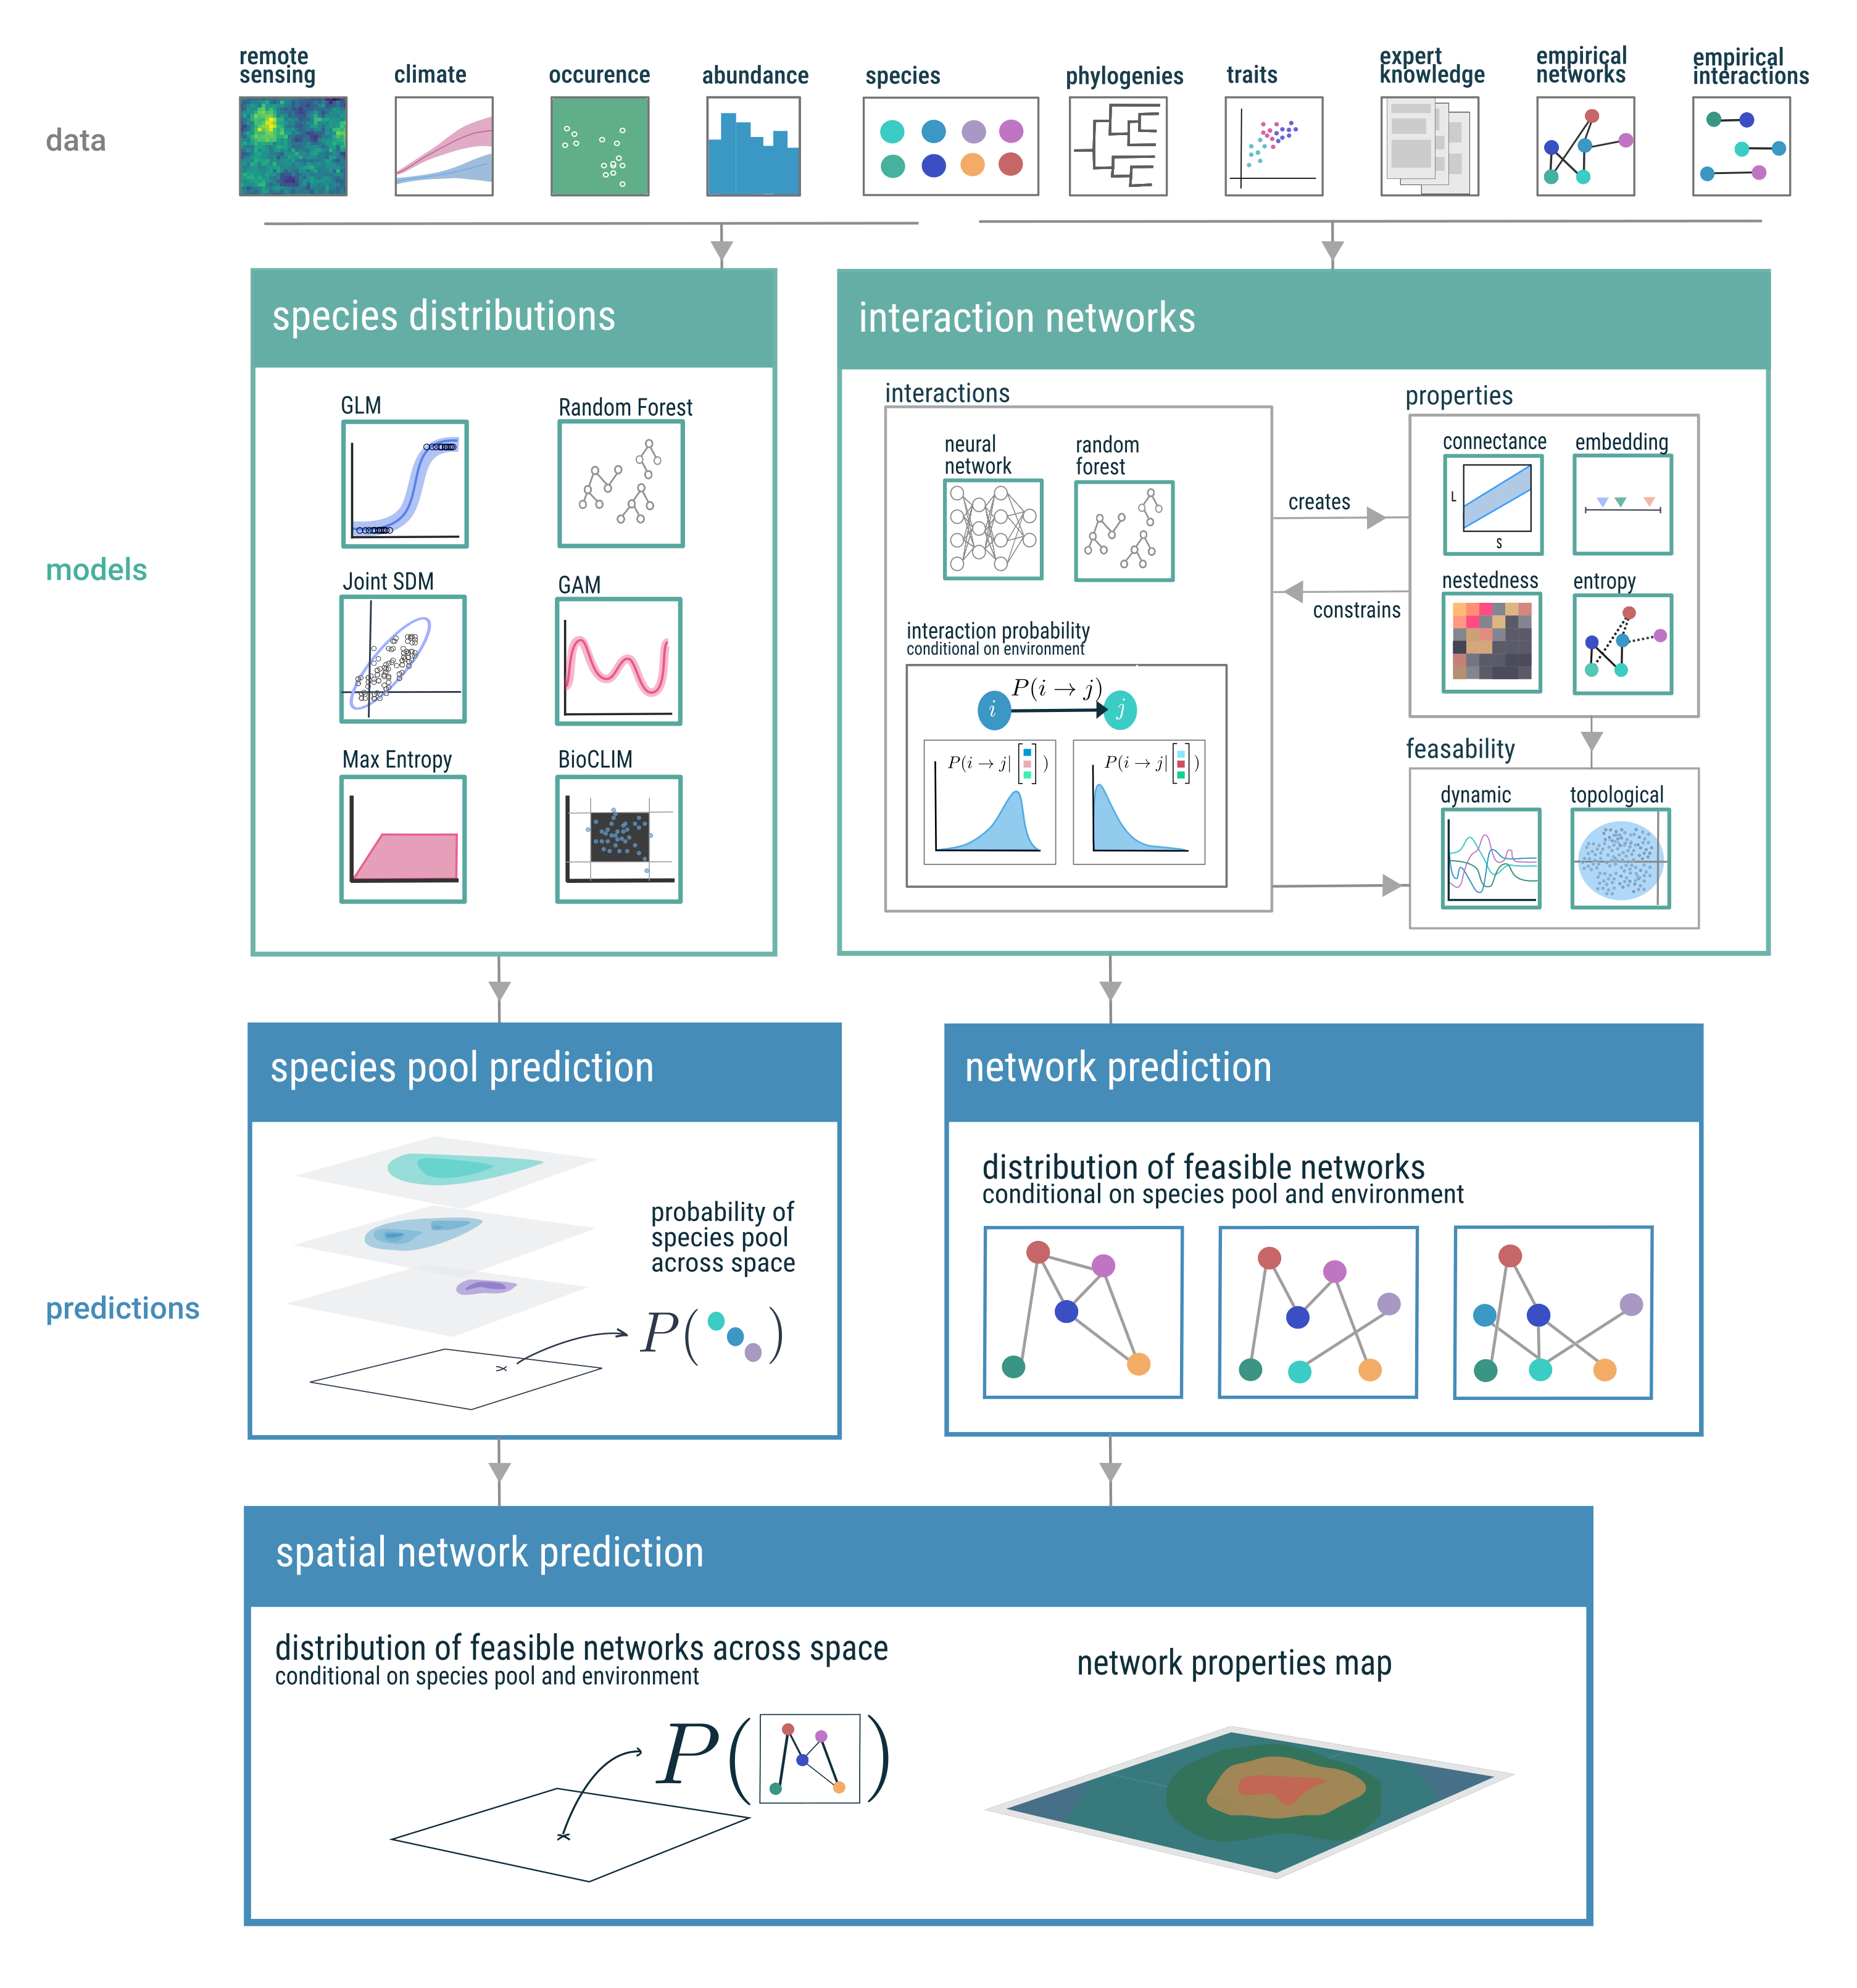
\includegraphics[width=\textwidth]{figures/concept_v6.png}
    \caption{A conceptual roadmap highlighting key areas for the prediction
of ecological networks. Starting with the input of data from multiple
sources, followed by a modelling framework for ecological networks and
the landscape, which are then ultimately combined to allow for the
prediction of spatially explicit networks.}
    \label{fig:conceptual}
\end{figure}

\subsection{Challenges: constraints on
predictions}\label{challenges-constraints-on-predictions}

\subsubsection{Ecological network data are scarce and hard to
obtain}\label{ecological-network-data-are-scarce-and-hard-to-obtain}

At the moment, prediction of species interactions is made difficult by
the limited availability of data. Although we have seen a growth in
species occurrence data, this growth is much slower for ecological
interactions because species interactions are challenging to sample
comprehensively \cite{Bennett2019PotPit, Jordano2016SamNet} and
sampling methodology has strong effects on the resulting data
\cite{deAguiar2019RevBia}. In turn, the difficulty of sampling
interactions can lead to biases in our understanding of network
structure \cite{deAguiar2019RevBia}. This knowledge gap has motivated a
variety of approaches to deal with interactions in ecological research
based on assumptions that do not always hold, such as the assumption
that co-occurrence is equivalent to meaningful interaction strength
\cite{Blanchet2020CooNot}. Spatial biases in data coverage are prevalent
at the global scale (with South America, Africa and Asia being
under-represented) and different interaction types show biases towards
different biomes \cite{Poisot2021GloKno}. These ``spatial gaps'' serve
as a limitation to our ability to confidently make predictions when
accounting for real-world environmental conditions, especially in
environments for which there are no analogous data.

Further, empirical estimation of interaction \emph{strength} is highly
prone to bias as existing data are usually summarised at the taxonomic
scale of the species or higher, thereby losing information that
differentiates the strength in per-individual interactions from the
strength of a whole species interaction \cite{Wells2013SpeInt}.
Empirical estimations of interaction strength are still crucial
\cite{Novak2008EstNon}, but are a hard task to quantify in natural
communities \cite{Wootton1997EstTes, Sala2002ComDis,
Wootton2005MeaInt}, especially as the number of species composing
communities increases, compounded by the possibility of higher-order
interactions or non-linear responses in interactions
\cite{Wootton2005MeaInt}. Further, interaction strength is often
variable and context dependent and can be influenced by
density-dependence and spatio-temporal variation in community
composition \cite{Wootton2005MeaInt}.

\subsubsection{Powerful predictive tools work better on large data
volumes}\label{powerful-predictive-tools-work-better-on-large-data-volumes}

This scarcity of data limits the range of computational tools that can
be used by network ecologists. Most deep learning methods, for instance,
are very data expensive. The paucity of data is compounded by a
collection of biases in existing datasets. Species interaction data are
typically dominated by food webs, pollination, and host-parasite
networks \cite{Ings2009EcoNet, Poisot2020EnvBia}. This could prove to
be a limiting factor when trying to understand or predict networks of
underrepresented interaction types or when trying to integrate networks
of different types \cite{Fontaine2011EcoEvo}, especially given their
inherent structural variation \cite{Michalska-Smith2019TelEco}. This
stresses the need for an integrated, flexible, and data-efficient set of
computational tools which will allow us to predict ecological networks
accurately from existing and imperfect datasets, but also enable us to
perform model validation and comparison with more flexibility than
existing tools. We argue that \autoref{fig:example} is an example of the promise
of these tools \emph{even} when facing datasets of small size. The
ability to extract and engineer features also serves to bolster our
predictive power. Although it may be tempting to rely on approaches like
bootstrapping to estimate the consistency of the predictions, we are
confronted with the issues of low data volume and data bias---that we
are more likely to observe interactions between some pairs of species
(i.e.~those that co-occur often, e.g. \cite{Cazelles2015TheSpe}, and those
with higher relative abundance, e.g. \cite{Vazquez2009UniPat}). This
introduces risk in training models on pseudo-replicated data. In short,
the current lack of massive datasets must not be an obstacle to
prediction; it is an ideal testing ground to understand how little data
is sufficient to obtain actionable predictions, and how much we can rely
on data inflation procedures to reach this minimal amount.

\subsubsection{Scaling-up predictions requires scaled-up
data}\label{scaling-up-predictions-requires-scaled-up-data}

We are also currently limited by the level of biological organisation at
which we can describe ecological networks. For instance, our
understanding of individual-based networks (e.g., \cite{Araujo2008NetAna,
Tinker2012StrMec} is still in its infancy \cite{Guimaraes2020StrEco}
and acts as a resolution-limit. Similarly, the resolution of
environmental (or landscape) data also limits our ability to predict
networks at small scales, although current trends in remote sensing
would suggest that this will become less of a hindrance with time
\cite{Makiola2020KeyQue}. Ecosystems are a quintessential
complex-adaptive-system \cite{Levin1998EcoBio} with a myriad of
processes at different spatial, temporal, and organisational scales that
influence and respond to one another. Understanding how the product of
these different processes drive the properties of ecosystems across
different scales remains a central challenge of ecological research, and
we should strive to work on methods that will integrate different
empirical ``snapshots'' of this larger system.

\subsection{Opportunities: an emerging ecosystem of open tools and
data}\label{opportunities-an-emerging-ecosystem-of-open-tools-and-data}

\subsubsection{Data are becoming more
interoperable}\label{data-are-becoming-more-interoperable}

The acquisition of biodiversity and environmental data has tremendously
increased over the past decades thanks to the rise of citizen science
\cite{Dickinson2010CitSci} and of novel technology
\cite{Stephenson2020TecAdv}, including wireless sensors
\cite{Porter2005WirSen}, next-generation DNA sequencing
\cite{Creer2016EcoSF}, and remote sensing \cite{Skidmore2015AgrBio,
Lausch2016LinEar}. Open access databases, such as
\href{https://www.gbif.org/}{GBIF} (for biodiversity data),
\href{https://www.ncbi.nlm.nih.gov/}{NCBI} (for taxonomic and genomics
data), \href{https://www.treebase.org/treebase-web/home.html}{TreeBASE}
(for phylogenetics data), \href{https://icestes.github.io/}{CESTE}
\cite{Jeliazkov2020GloDat} (for metacommunity ecology and species traits
data), and \href{https://www.worldclim.org/data/bioclim.html}{WorldClim}
(for bioclimatic data) contain millions of data points that can be
integrated to monitor and model biodiversity at the global scale. For
species interactions data, at the moment
\href{https://mangal.io/#/}{Mangal} is the most comprehensive open
database of published ecological networks \cite{Poisot2016ManMak}, and
\href{https://www.globalbioticinteractions.org/about}{GloBI} is an
extensive database of realised and potential species interactions
\cite{Poelen2014GloBio}. Developing standard practices in data
integration and quality control \cite{Kissling2018BuiEss} and in
next-generation biomonitoring (NGB; \cite{Makiola2020KeyQue}) would
improve our ability to make reliable predictions of ecosystem properties
on increasing spatial and temporal scales. The advancement of prediction
techniques coupled with a movement towards standardising data collection
protocols (e.g. \cite{Perez-Harguindeguy2013NewHan} for plant functional
traits) and metadata (e.g.
\href{https://www.tdwg.org}{DarwinCore})---which facilitates
interoperability and integration of datasets---as well as a growing
interest at the government level \cite{Scholes2012BuiGlo} paints a
positive picture for data access and usability in the coming years.

\subsubsection{Machine learning tools are becoming more
accessible}\label{machine-learning-tools-are-becoming-more-accessible}

This effort is also supported by a thriving ecosystem of data sources
and novel tools. ML methods can often be more flexible and perform
better than classical statistical methods, and can achieve a very high
level of accuracy in many predictive and classification tasks in a
relatively short amount of time (e.g., \cite{Cutler2007RanFor,
Krizhevsky2017ImaCla}). Increasing computing power combined with
recent advances in machine learning techniques and applications shows
promise in ecology and environmental science (see \cite{Christin2019AppDee}
for an overview). Moreover, ongoing developments in deep learning are
aimed at improvement in low-data regimes and with unbalanced datasets
\cite{Antoniou2018DatAug, Chawla2010DatMin}. Considering the current
biases in network ecology \cite{Poisot2021GloKno} and the scarcity of
data of species interactions, the prediction of ecological networks will
undoubtedly benefit from these improvements. Machine learning methods
are emerging as the new standard in computational ecology in general
\cite{Olden2008MacLea, Christin2019AppDee}, and in network ecology in
particular \cite{Bohan2017NexGlo}, as long as sufficient, relevant data
are available. Many studies have used machine learning models
specifically with ecological interactions. Relevant examples include
species traits used to predict interactions and infer trait-matching
rules \cite{Desjardins-Proulx2017EcoInt, Pichler2020MacLea}, automated
discovery of food webs \cite{Bohan2011AutDis}, reconstruction of
ecological networks using next-generation sequencing data
\cite{Bohan2017NexGlo}, and network inference from presence-absence data
\cite{Sander2017EcoNet}. As many ecological and evolutionary processes
underlie species interactions and the structure of their ecological
networks (\emph{e.g.,} \cite{Vazquez2009UniPat, Segar2020RolEvo}, it can be
difficult to choose relevant variables and model species interactions
networks explicitly. A promising application of machine learning in
natural sciences is Scientific-Machine Learning (SciML), a framework
that combines machine learning with mechanistic models
\cite{Chuang2018AdvCon, Rackauckas2020UniDif}.

\section{A primer on predicting ecological
networks}\label{a-primer-on-predicting-ecological-networks}

Within the constraints outlined in the previous section, we now provide
a primer on the background concepts necessary to build predictive models
of species interaction networks, with a focus on using machine learning
approaches in the modelling process. As @fig:conceptual illustrates,
this involves a variety of numerical and computational approaches;
therefore, rather than an exhaustive summary, we aim to convey a
high-level understanding that translates the core concepts into their
application to ecological networks.

\subsection{Models}\label{models}

\subsubsection{What is a predictive
model?}\label{what-is-a-predictive-model}

Models are used for many purposes, and the term ``model'' itself
embodies a wide variety of meanings in scientific discourse. All models
can be thought of as a function, \(f\), that takes a set of inputs \(x\)
(also called features, descriptors, or independent variables) and
parameters \(\theta\), and maps them to predicted output states \(y\)
(also called label, response, or dependent variable) based on the input
to the model: \(y=f(x,\theta)\).

A given model \(f\) can be used for either descriptive or predictive
purposes. Many forms of scientific inquiry are based around using models
\emph{descriptively}, a practice also called inference, the inverse
problem, fitting a model, or training a model \cite{Stouffer2019AllEco}.
In this context, the goal of using a model is to estimate the
parameters, \(\theta\), that best explain a set of empirical
observations, \(\{\hat{x}, \hat{y}\}\). In some cases, these parameter
values are themselves of interest (e.g., the strength of selection,
intrinsic growth rate, dispersal distance), but in others cases, the
goal is to compare a set of competing models \(f_1, f_2, \dots\) to
determine which provides the most parsimonious explanation for a
dataset. The quantitative representation of ``effects'' in these
models---the influence of each input on the output---is often assumed to
be linear, and within the frequentist world-view, the goal is often to
determine if the coefficient corresponding with an input is non-zero to
determine its ``significance'' (often different from its ecological
relevance \cite{Martinez-Abrain2008StaSig}) in influencing the outcome.

Models designed for inference have utility---descriptive models of
networks can reveal underlying mechanisms that structure ecological
communities, given a proper null model \cite{Connor2017UsiNul}. However,
in order for ecology to develop as a predictive science
\cite{Evans2012PreEco}, interest has grown in developing models that are
used not just for description of data, but also for prediction.
Predictive models are based in \emph{the forward problem}, where the aim
is to predict new values of the output \(y\) given an input \(x\) and
our estimate value of \(\theta\) \cite{Stouffer2019AllEco}. Because the
forward problem relies on an estimate of \(\theta\), then, the problem
of inference is nested within the forward problem (Fig.\ref{fig:models}): working
towards a predictive view of ecological networks will give us the needed
tools to further our understanding of them.

\begin{figure}[h]
    \centering
    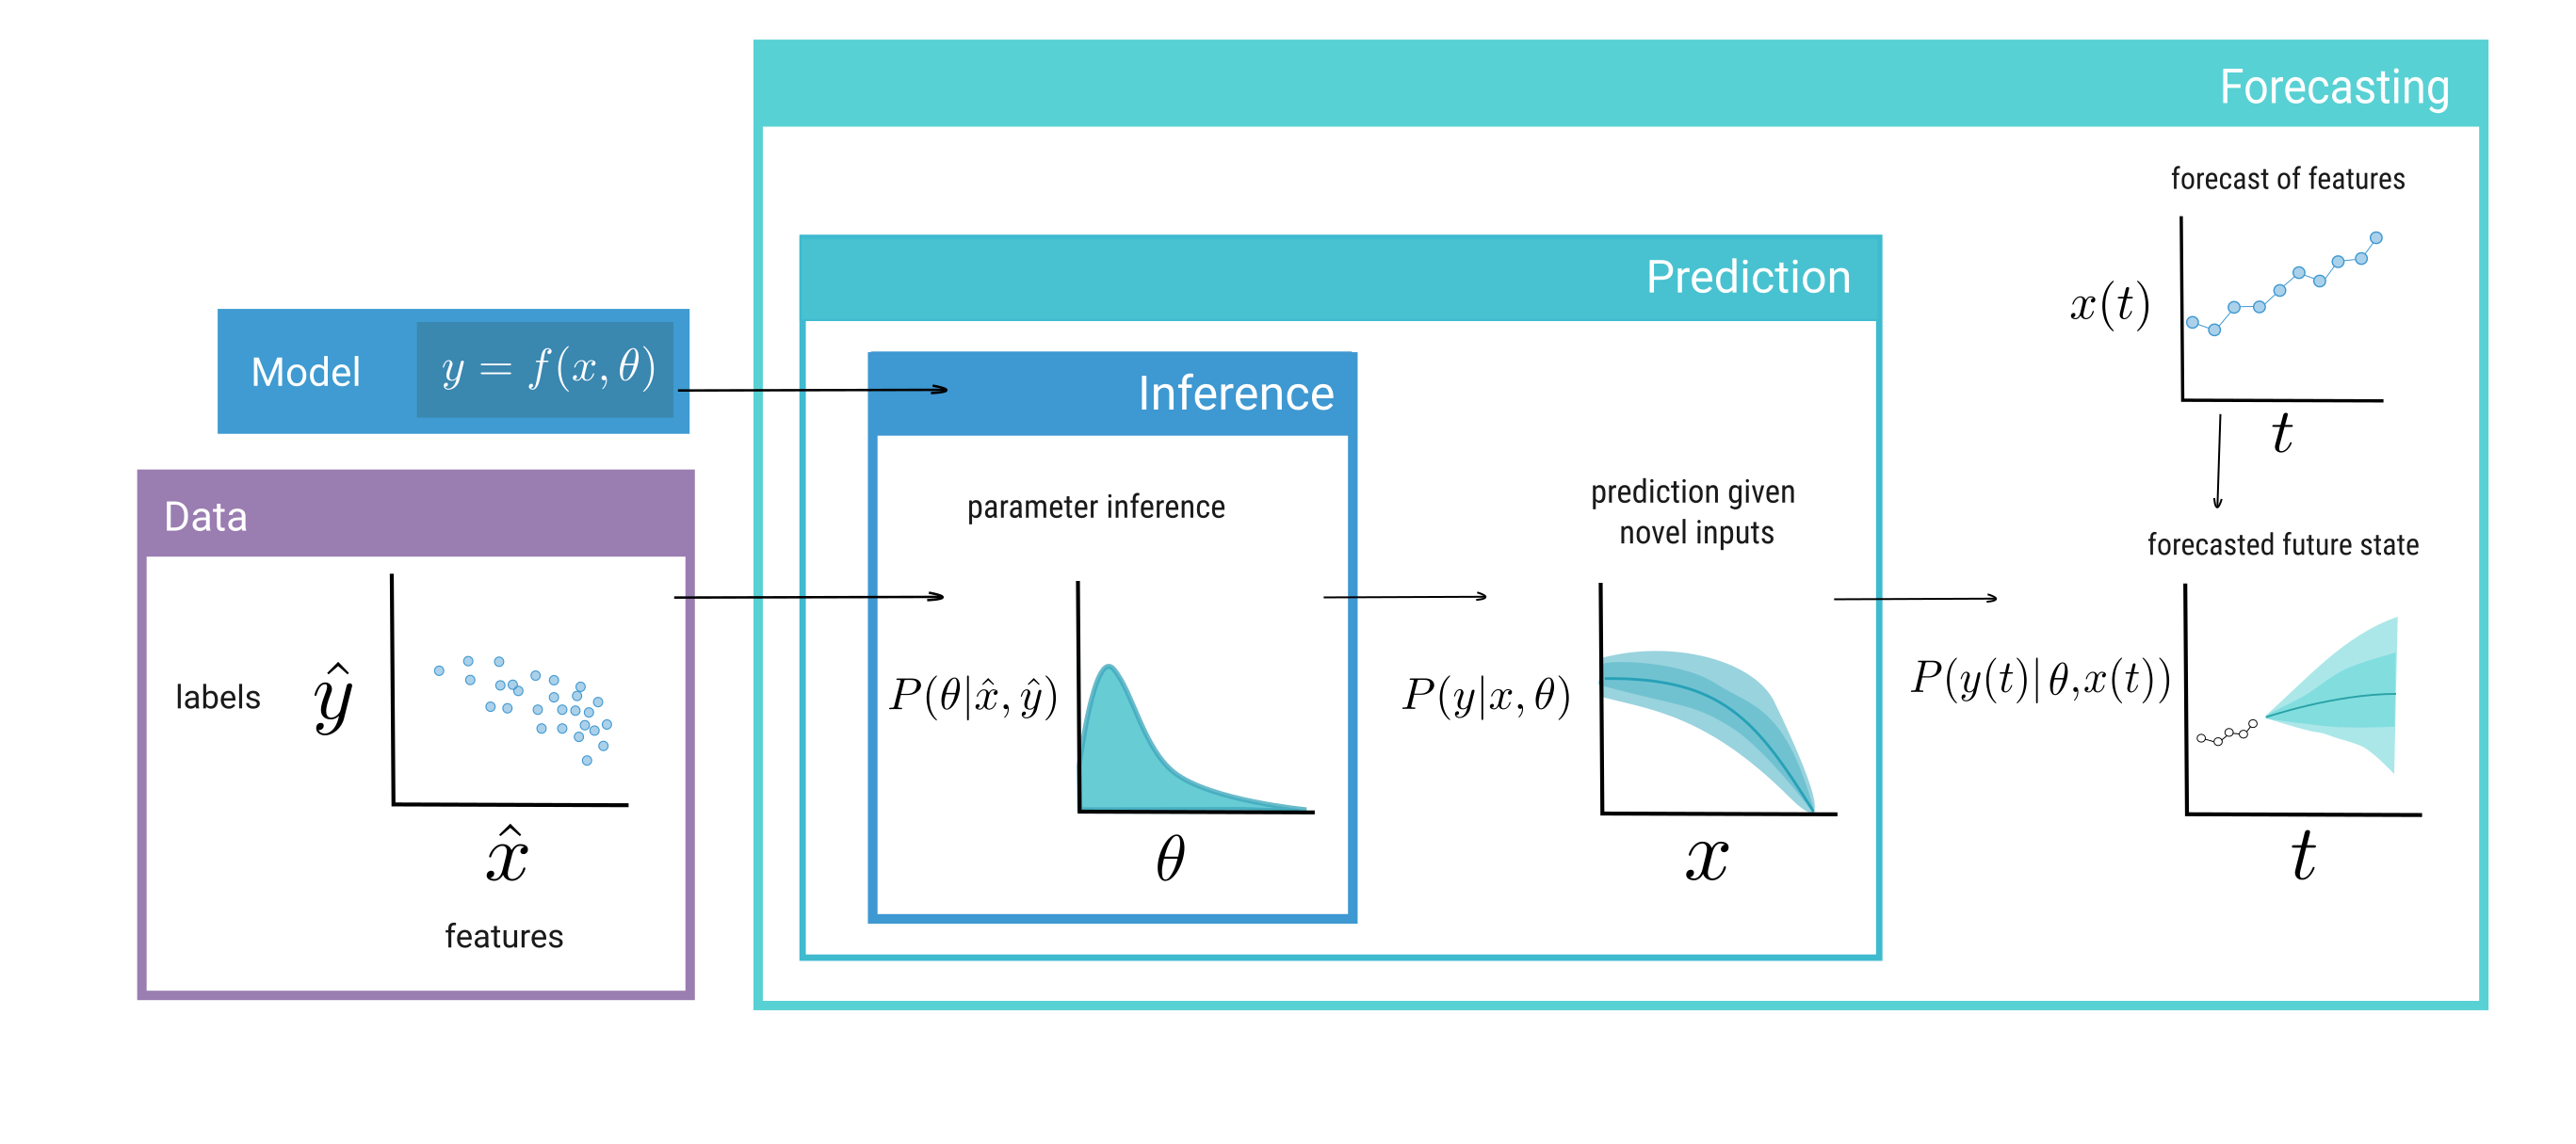
\includegraphics[width=\textwidth]{figures/forecasting_v4.png}
    \caption{The nested nature of developing predictive and forecasting
models, showcases the \emph{forward problem} and how this relies on a
hierarchical structure of the modelling process. The choice of a
specific modelling technique and framework, as well as the data retained
to be part of this model, proceeds directly from our assumptions about
which ecological mechanisms are important in shaping both extant and
future data.}
    \label{fig:models}
\end{figure}

\subsubsection{What do you need to build a predictive
model?}\label{what-do-you-need-to-build-a-predictive-model}

To build a predictive model, one needs the following: first,
\textbf{data}, split into features \(\hat{x}\) and labels \(\hat{y}\)
(@fig:models). Second, a \textbf{model} \(f\), which maps features \(x\)
to labels \(y\) as a function of parameters \(\theta\),
i.e.~\(y = f(x, \theta)\). Third, a \textbf{loss function}
\(L(\hat{y}, y)\), which describes how far a model's prediction \(y\) is
from an empirical value \(\hat{y}\). Lastly, \textbf{priors} on
parameters, \(P(\theta)\), which describe the modeller's \emph{a priori}
belief about the value of the parameters; rather than making an analysis
implicit, specifying priors has the merit of making the modeller's
assumptions explicit, which is a most desirable feature when
communicating predictions to stakeholders
\cite{Spiegelhalter2000BayMet}. Often an important step before fitting a
model is feature engineering: adjusting and reworking the features to
better uncover feature-label relationships \cite{Kuhn2019FeaEng}. This
can include projecting the features into a lower dimensional space, as
we did through a probabilistic PCA in the case study, or removing the
covariance structure using a Whitening approach. Then, when a model is
fitted (synonymous with parameter inference or the inverse problem, see
\autoref{fig:models}), a fitting algorithm attempts to estimate the values of
\(\theta\) that minimises the mean value of loss function
\(L(\hat{y},y)\) for all labels \(\hat{y}\) in the provided data \(Y\).
In a Bayesian approach, this typically relys on drawing candidate
parameter values from priors and applying some form of sampling to
generate a posterior estimate of parameters,
\(P(\theta | \hat{x}, \hat{y})\). In the training of neural networks,
this usually involves some form of error back-propagation across the
edges in order to tune their weights, and the biases of each nodes.

\subsubsection{How do we validate a predictive
model?}\label{how-do-we-validate-a-predictive-model}

After we fit a model, we inevitably want to see how ``good'' (meaning,
``fit for purpose'') it is. This process can be divided into two parts:
(i)) model selection, where the modeller chooses from a set of possible
models and (ii) model assessment, where the modeller determines the
performance characteristics of the chosen model \cite{Hastie2009EleSta}.

In the context of \emph{model selection}, a naïve initial approach is to
simply compute the average error between the model's prediction and the
true data we have, and choose the model with the smallest
error---however this approach inevitably results in \emph{overfitting}.
One approach to avoid overfitting is using information criteria (e.g.,
AIC, BIC, MDL) based around the heuristic that good models maximise the
ratio of information provided by the model to the number of parameters
it has. However, when the intended use-case of a model is prediction the
relevant form of validation is \emph{predictive accuracy}, which should
be tested with \emph{cross-validation}. Cross-validation methods divide
the original dataset into two---one which is used to fit the model
(called the \emph{training} set) and one used to validate its predictive
accuracy on the data that it hasn't ``seen'' yet (called the \emph{test}
set) \cite{Bishop2006PatRec}. This procedure is often repeated across
different test and training subdivisions of the dataset (either picked
randomly or stratified by some criteria, like balance between positive
and negative interactions in the case study) to determine the
uncertainty associated with our measurement due to our choice of test
and training sets \cite{Arlot2010SurCro}, in the same conceptual vein as
data bootstrapping: the mean value of the validation metric gives an
overall estimate of its performance, and the variance around this mean
represents the effect of using different data for training and testing.
In a robust model/dataset combination, we expect this variance to be
low, although there are no prescriptive guidelines as to how little
variance is acceptable; the choice of whether to use a model is often
left to the best judgement of the modeller.

We still have to define what \emph{predictive accuracy} means in the
context of interaction network prediction. In the proof-of-concept, we
used a neural-network to perform binary classification by predicting the
presence/absence of an interaction between any two species. There are
two ways for the model to be right: the model predicts an interaction
and there is one (a \emph{true positive} (TP)), or the model predicts no
interaction and there isn't one (a \emph{true negative} (TN)).
Similarly, there are two ways for the model to be wrong: the model
predicts an interaction which does not exist (a \emph{false positive}
(FP)), or the model predicts no interaction but it does exist (a
\emph{false negative} (FN)).

A naïve initial approach to measure how well a model does is
\emph{accuracy}, i.e. the proportion of values it got correct. However,
consider what we know about interaction networks: they are often very
sparse, with connectance usually below a third \cite{Cohen1990ComFoo}.
If we build a model that always guesses there will be no interaction
between two species, it will be correct in the majority of cases because
the majority of potential interactions in a network typically do not
exist. Therefore this ``empty-matrix'' model would always have an
\emph{accuracy} of \(1-C\), where \(C\) is the observed connectance,
which would almost always be greater than 50\%. Understanding model
performance within sensitivity-specificity space may be more
informative, where sensitivity evaluates how good the model is at
predicting true interactions (True Positive Rate) and specificity refers
to the prediction of true ``non-interactions'' (True Negative Rate). It
must be noted that in ecological networks, there is no guarantee that
the ``non-interactions'' (assumed true negatives) in the original
dataset are indeed true negatives \cite{Jordano2016ChaEco,
Jordano2016SamNet}. This can result in the positive/negative values,
and the false omission/discovery being artificially worse, and
specifically decrease our confidence in predicted interactions.

In response to the general problem of biases in classifiers, many
metrics have been proposed to measure binary-classifiers
\cite{Gu2009EvaMea, Drummond2006CosCur} and are indicative of how well
the model performs with regards to some aspect of accuracy, sensitivity,
specificity and/or precision (\autoref{tbl:validation}). Ultimately the choice of
metric will depend on the intended use of the model: there is not a
single definition of ``success'', but rather different interpretation of
what sources of error are acceptable for a given application.

\begin{table}[h!]
\resizebox{\textwidth}{!}{
\centering
\begin{tabular}{||c c c c||} 
 \hline
 Name & Value & Success & Description \\ [0.2ex] \hline\hline
 Random accuracy & 0.56 & & Fraction of correct predictions if the
classifier is random \\ 
 Accuracy & 0.81 & \(\rightarrow 1\) & Observed fraction of correct
predictions \\
 Balanced accuracy & 0.80 & \(\rightarrow 1\) & Average fraction of
correct positive and negative predictions \\
& & & \\
True Positive Rate & 0.77 & \(\rightarrow 1\) & Fraction of interactions
predicted \\
True Negative Rate & 0.83 & \(\rightarrow 1\) & Fraction of
non-interactions predicted \\
False Positive Rate & 0.16 & \(\rightarrow 0\) & Fraction of
non-interactions predicted as interactions \\
False Negative Rate & 0.22 & \(\rightarrow 0\) & Fraction of
interactions predicted as non-interactions \\
& & & \\
ROC-AUC & 0.86 & \(\rightarrow 1\) & Proximity to a perfect prediction
(ROC-AUC=1) \\
Youden's J & 0.60 & \(\rightarrow 1\) & Informedness of predictions
(trust in individual prediction) \\
Cohen's \(\kappa\) & 0.58 & \(\ge 0.5\) & \\
& & & \\
Positive Predictive Value & 0.66 & \(\rightarrow 1\) & Confidence in
predicted interactions \\
Negative Predictive Value & 0.89 & \(\rightarrow 1\) & Confidence in
predicted non-interactions \\
False Omission Rate & 0.10 & \(\rightarrow 0\) & Expected proportion of
missed interactions \\
False Discovery Rate & 0.33 & \(\rightarrow 0\) & Expected proportion of
wrongly imputed interactions \\ [0.2ex] 
 \hline
\end{tabular}
}
\caption{Overview of the validation statistics applied to the case
study, alongside the criteria indicating a successful classifier and a
guide to interpretation of the values. Taken together, these validation
measures indicate that the model performs well, especially considering
that it is trained from a small volume of data.}
\label{tbl:validation}
\end{table}

In the machine learning literature, a common way of visualising this
extensive list of possible metrics is through the use of ROC
(receiver-operating-characteristic; False Positive Rate on the x-axis,
and True Positive Rate on the y-axis) and PR (precision-recall;
True-Positive-Rate on the x-axis, Positive-predictive-value on the
y-axis) curves (see \autoref{fig:example}). These curves are generated by
considering a continuum of thresholds of classifier acceptance, and
computing the values of ROC/PR metrics for each value of the threshold.
The area-under-the-curve (AUC) is then used as a validation metric and
are typically called AUC-ROC (Area-Under-the-Curve
Receiver-Operator-Curve) and AUC-PR (Area-Under-the-Curve
Precision-Recall) (e.g.~ROC-AUC in Table \ref{tbl:validation}). These measures have
the unstated assumption that the training and testing set are
``correct'', or at least correct enough that the number of true/false
positive/negatives are meaningful; although should this assumption be
true, there would be no need for any predictive approach -- but it is a
well established fact that machine learning systems are resilient to
even relatively high uncertainties in the data \cite{Halevy2009UnrEff}.

\subsection{Networks and interactions as predictable
objects}\label{networks-and-interactions-as-predictable-objects}

\subsubsection{Why predict networks and interactions at the same
time?}\label{why-predict-networks-and-interactions-at-the-same-time}

Ecological networks are quite sparse, and larger networks tend to get
sparser \cite{MacDonald2020RevLin}; in other words, although networks
are composed of a set of interactions between species pairs, they also
form a much larger set of species pairs that do not interact. If we aim
to predict the structure of networks from the ``bottom-up''--- by
considering each pairwise combination of \(S\) different species---we
are left with \(S^2\) interaction values to estimate, a majority of
which will be 0. Instead, we can use our existing understanding of the
mechanisms that structure ecological networks to whittle down the set of
feasible adjacency matrices, thereby reducing the amount of information
we must predict, and making the problem of predicting interactions less
daunting. The processes that structure ecological networks do not only
occur at the scale of interactions---there are also processes at the
network level which limit what interactions (or how many) are realistic.
The realised structure of a network is the synthesis of the interactions
forming the basis for network structure, and the network structure
refining the possible interactions---``Part makes whole, and whole makes
part'' \cite{Levins1987DiaBio}.

Another argument for the joint prediction of networks and interactions
is to reduce circularity and biases in the predictions. As an example,
models like linear filtering \cite{Stock2017LinFil} generate
probabilities of non-observed interactions existing, but do so based on
measured network properties. Some recent models make interaction-level
predictions (\emph{e.g.,} \cite{Gravel2019BriElt}); these are not unlike stacked
species distribution models, which are individually fit, but
collectively outperformed by joint models or rule-based models
\cite{Zurell2020TesSpe}. By relying on adequate testing of model
performance of biases (\emph{i.e.,} optimising not only accuracy, but paying
attention to measures like false discovery and false omission rates),
and developing models around a feedback loop between network and
interaction prediction, it is likely that the quality of the predicted
networks will be greatly improved compared to current models.

\subsubsection{What network properties should we use to inform our
predictions of
interactions?}\label{what-network-properties-should-we-use-to-inform-our-predictions-of-interactions}

There are many dimensions of network structure \cite{Delmas2018AnaEco},
yet there are two arguments to support basing network prediction around
a single property: \emph{connectance} (the ratio of actual edges to
possible edges in the network). First, connectance is ecologically
informative---it relates to resilience to invasion \cite{Baiser2010ConDet,
Smith-Ramesh2016GloSyn}, can increase robustness to extinction in
food webs \cite{Dunne2002NetStr}, while decreasing it in mutualistic
networks \cite{Vieira2015SimSto}, and connectance relates to network
stability \cite{Landi2018ComSta}. Second, most (if not all) network
properties covary with connectance \cite{Poisot2014WheEco,
Dunne2002FooStr}.

Within the network science literature, there are numerous methods for
predicting edges based on network properties (\emph{e.g.,} block models
\cite{Yen2020ComDet} based on modularity, hierarchical models
\cite{Kawakatsu2021EmeHie} based on embedding, etc.). However, in the
context of species interaction networks, these properties often co-vary
with connectance. As a result we suggest that using connectance as the
primary property of interest is most likely to be practical to formulate
at the moment. We have models to estimate species richness over space
\cite{Jenkins2013GloPat}, and because we can predict connectance from
species richness alone \cite{MacDonald2020RevLin}, we can then derive
distributions of network properties from richness estimates, that can
serve to penalise further models that formulate their predictions at the
scale of each possible interaction.

\subsubsection{How do we predict how species that we have never observed
together will
interact?}\label{how-do-we-predict-how-species-that-we-have-never-observed-together-will-interact}

A neutral approach to ecological interactions would assume the
probability of an interaction to mirror the relative abundance of both
species, and would be unaffected by trait variation
\cite{Poisot2015SpeWhy, Pichler2020MacLea}; more accurately, a neutral
assumption states that the relative abundances are sufficient to predict
the structure of networks, and this view is rather well supported in
empirical and theoretical systems \cite{Canard2012EmeStr,
Canard2014EmpEva}. However, functional-trait based proxies could
enable better predictions of ecological interactions
\cite{Cirtwill2018FeeEnv, Cirtwill2019QuaFra, Bartomeus2016ComFra,
Bartomeus2013UndLin}. Selection on functional traits could cause
interactions to be conserved at some evolutionary scales, and therefore
predictions of interaction could be informed by phylogenetic analyses
\cite{Davies2021EcoRed, Elmasri2020HieBay, Gomez2010EcoInt}.
Phylogenetic matching in bipartite networks is consistent across scales
\cite{Poisot2018IntRet}, even in the absence of strong selective
pressure \cite{Coelho2017NeuBio}.

A separate family of methods are based on network embedding (as in the
proof-of-concept). A network embedding projects each node of the network
into a lower-dimensional latent space. Previous explorations of the
dimensionality of food webs have revealed that a reduced number of
dimensions (7) was sufficient to capture most of their structure
\cite{Eklof2013DimEco}; however, recent quantifications of the
complexity of the embedding space of bipartite ecological networks found
a consistent high complexity \cite{Strydom2021SvdEnt}, suggesting that
the precise depth of embedding required may vary considerably across
systems. Embeddings enables us to represent the structure of a network,
which previously required the \(S^2\) dimensions of an adjacency matrix,
with a smaller number of dimensions. The position of each node in this
lower dimensional space is then treated as a latent measurement
corresponding to the role of that species in the network (\emph{e.g.,}
\cite{Poisot2021ImpMam}, where a network of about 1500 species was most
accurately described using 12 dimensions). Species close together in
the latent space should interact with similar set of species
\cite{Rossberg2006FooWeb, Rohr2010ModFoo}. However, these models are
sensitive to sampling biases as they are limited to species for which
there is already interaction data, and as a result a methodological
breakthrough is needed to extend these models to species for which there
is little or no interaction data.

\subsubsection{How do we quantify interaction
strength?}\label{how-do-we-quantify-interaction-strength}

Species interaction networks can also be used as a means to quantify and
understand \emph{interaction strength}. Interaction strength, unlike the
qualitative presence or absence of an interaction, is a continuous
measurement which attempts to quantify the effect of one species on
another. This results in weighted networks representing different
patterns of `flows' between nodes -- which can be modelled in a variety
of ways \cite{Borrett2019WalPar}. Interaction strength can generally be
divided into two main categories (as suggested by \cite{Berlow2004IntStr}): 1)
the strength of an interaction between individuals of each species, or
2) the effect that changes in one species population has on the dynamics
of the other species. It can be measured as the effect over a period of
time (in the units of biomass or energy flux \cite{Barnes2018EneFlu,
Brown2004MetThe}) or the relative importance of one species on
another \cite{Heleno2014EcoNet, Berlow2004IntStr, Wootton2005MeaInt}.
One recurring observation is that networks are often composed of many
weak interactions and few strong interactions \cite{Berlow2004IntStr}.
The distribution of interaction strength within a network effects its
stability \cite{Neutel2002StaRea, Ruiter1995EnePat} and functioning
\cite{Duffy2002BioEco, Montoya2003FooWeb}, and serves to benefit
multi-species models \cite{Wootton2005MeaInt}. Alternatively,
understanding flow in modules within networks can aid in understanding
the organisation of networks \cite{Farage2021IdeFlo, Montoya2002SmaWor}
or the cascading effects of perturbations \cite{Gaiarsa2019IntStr}.

In some systems, quantifying interaction strength is relatively
straightforward; this includes a lot of host-parasite systems. For
example, freshwater cyprinid fish can be divided in micro-habitats
(fins, skin, digestive system, gill subsections) and the parasites
counted in each of these micro-habitats, giving within-host resolution
\cite{Simkova2002AbuRel}; marine sparids and labrids have similarly been
studied this way, see notably \cite{Sasal1999ComStr,
Desdevises2006DetPar, Morand2002InvPat}. In some cases, within-host
assessments of interaction strengths can reveal macro-ecological events,
like in the conservatism of micro-habitat use in amphibian hosts by
helminths \cite{Badets2011CorEar}. Even ectoparasites can provide
reliable assessments of interaction strength; for example, when rodent
hosts are minimally disturbed during capture, fine combing of their fur
will result in exhaustive ectoparasites inventories
\cite{Hadfield2014TalTwo, Karbowiak2019ComImm, Matthee2020DivDis,
Sanchez2014PosCoo, Dickinson2020SamSca}. Parasites have the
desirable property of usually remaining intact within their host during
the interaction, as opposed to prey items as can be recovered through
\emph{e.g.,} gut content analysis or stable isotopes
\cite{Macias-Hernandez2018MolGut, Schmid-Araya2016TroPos}. As network
ecology is starting to explore the use of predictive models, leading up
to forecasting, we argue that host-parasite systems can provide data
that are reliable and trustworthy enough that they can become the
foundations for methodological development and benchmark studies,
thereby providing more information about host-parasite systems and
supporting the technical development of the field.

Yet in most situations, much like quantifying the occurrence of an
interaction, quantifying interaction \emph{strength} in the field is
challenging in the majority of systems, and one must often rely on
proxies. In some contexts, interaction strength can be estimated via
functional foraging \cite{Portalier2019MecPre}, where the primary basis
for inferring interaction is foraging behaviour like searching, capture
and handling times. In food-webs, metabolic based models use body mass,
metabolic demands, and energy loss to infer energy fluxes between
organisms \cite{Yodzis1992BodSiz, Berlow2009SimPre}. In addition,
food-web energetics models can be incorporated at various resolutions
for a specific network, ranging from individual-based data to more
lumped data at the species level or trophic group, depending on data
availability \cite{Barnes2018EneFlu, Berlow2009SimPre}. Taken together,
these considerations impose too many constraints on predicting
continuous interaction strength at the moment, resulting in our primary
focus in binary present/absent interactions within this manuscript.

\subsubsection{How do we determine what interaction networks are
feasible?}\label{how-do-we-determine-what-interaction-networks-are-feasible}

For several decades, ecologists have aimed to understand how networks of
many interacting species persist through time. The diversity-stability
paradox, first explored by \cite{May1974StaCom}, shows that under a neutral
set of assumptions ecological networks should become decreasingly stable
as the number of species increases. Yet, in the natural world we observe
networks of interactions that consist of far more species than May's
model predicts \cite{Albouy2019MarFis}. As a result, understanding what
aspects of the neutral assumptions of May's model are incorrect has
branched many investigations into the relationship between ecological
network structure and persistence \cite{Allesina2012StaCri}. These
assumptions can be split into dynamical assumptions and topological
assumptions. Topologically, we know that ecological networks are not
structured randomly. Some properties, like the aforementioned
connectance, are highly predictable \cite{MacDonald2020RevLin}.
Generative models of food-webs (based on network embeddings) fit
empirical networks more effectively than random models
\cite{Allesina2008GenMod}. These models have long used allometry as a
single-dimensional niche space---naturally we want to extend this to
traits in general. The second approach to stability is through
\emph{dynamics}. Early models of community dynamics rely on the
assumption of linear interaction effects, but in recent years models of
bioenergetic community dynamics have shown promise in basing our
understanding of energy flow in food-webs in the understood relationship
between allometry and metabolism \cite{Delmas2017SimBio}. An additional
consideration is the multidimensional nature of ``stability'' and
``feasibility'' (e.g.~resilience to environmental change vs extinctions)
\cite{Dominguez-Garcia2019UnvDim} and how different disturbances
propagate across levels of biological organisation \cite{Kefi2019AdvOur,
Gravel2016StaCom}. Recent approaches such as structural stability
\cite{Saavedra2017StrApp, Ferrera2016EffCom} allow us to think of
network feasibility in rigorous mathematical terms, which may end up as
usable parameters to penalise network predictions.

\subsubsection{What taxonomic scales are suitable for the prediction of
species
interactions?}\label{what-taxonomic-scales-are-suitable-for-the-prediction-of-species-interactions}

If we use different trait-based proxies to predict potential
interactions between species the choice of such proxies should be
theoretically linked to the taxonomic and spatial scale we are using in
our prediction \cite{Wiens1989SpaSca}. At some scales we can use
morphological traits of co-occurring species to assess the probability
of interaction between them \cite{Bartomeus2016ComFra}. On broader
taxonomic scales we can infer interaction probability through the
phylogenetic distance, assuming that functional traits themselves are
conserved \cite{Gomez2010EcoInt}. In this case, we can think of the
probability that one species will interact with another as the distance
between them in niche-space \cite{Desjardins-Proulx2017EcoInt}, and this
can be modelled by simulating neutral expectations of trait variation on
phylogenetic trees \cite{Davies2021EcoRed}. At the narrowest scales, we
may be interested in predicting behavioural traits like foraging
behaviour \cite{Bartomeus2016ComFra}, and at this scale we may need to
consider abundance's effect on the probability of an encounter
\cite{Wells2013SpeInt}.

\subsubsection{What about indirect and higher-order
interactions?}\label{what-about-indirect-and-higher-order-interactions}

Although network ecology often assumes that interactions go strictly
from one node to the other, the web of life is made up of a variety of
interactions. Indirect interactions---either higher-order interactions
between species, or interaction strengths that themselves interact ---
have gained interest in recent years \cite{Golubski2016EcoNet,
Golubski2011ModMod}. One mathematical tool to describe these
situations is hypergraphs: hypergraphs are the generalisation of a
graph, allowing a broad yet manageable approach to complex interactions
\cite{Carletti2020DynSys}, by allowing for particular interactions to
occur beyond a pair of nodes. An additional degree of complexity is
introduced by multi-layer networks \cite{Hutchinson2019SeeFor}.
Multi-layer networks include edges across ``variants'' of the networks
(timepoints, locations, or environments). These can be particularly
useful to account for the metacommunity structure
\cite{Gross2020ModMod}, or to understand how dispersal can inform
conservation action \cite{Albert2017AppNet}. Ecological networks are
intrinsically multi-layered \cite{Pilosof2017MulNat}. However,
\emph{prima facie}, increasing the dimensionality of the object we need
to predict (the multiple layers rather than a single network) makes the
problem more complicated. Yet, multi-layer approaches improve prediction
in social networks \cite{Jalili2017LinPre, Najari2019LinPre,
Yasami2018NovMul}, and they may prove useful in network ecology going
forward.

\subsection{Space}\label{space}

Although networks were initially used to describe the interactions
\emph{within} a community, interest in the last decade has shifted
towards understanding their structure and variation over space
\cite{Trojelsgaard2016EcoNet, Baiser2019EcoRul}, and has established
network ecology as an important emerging component of biogeography and
macroecology.

\subsubsection{How much do networks vary over
space?}\label{how-much-do-networks-vary-over-space}

Networks can vary across space either in their structural properties
(\emph{e.g.,} connectance or degree distribution) or in their composition
(identity of nodes and edges). Interestingly, variation in the
structural properties of ecological networks primarily responds to
changes in the size of the network. The number of links in ecological
networks scales with the number of species \cite{MacDonald2020RevLin,
Brose2004UniSpa}, and connectance and size drive the rest of network
structure \cite{Poisot2014WheEco, Dunne2002FooStr, Riede2010ScaFoo}.
Species turnover in space results in changes in the composition of
ecological networks. But, this is not the only reason network
composition varies \cite{Poisot2015SpeWhy}. Intraspecific variation can
result in interaction turnovers without changes in species composition
\cite{Bolnick2011WhyInt}. Similarly, changes in species abundances can
lead to variation in interaction strengths \cite{Canard2014EmpEva,
Vazquez2007SpeAbu}. Variation in the abiotic environment and indirect
interactions \cite{Golubski2016EcoNet} could modify the occurrence and
strength of individual interactions. Despite this, empirical networks
tend to share a common backbone \cite{Mora2018IdeCom} and functional
composition \cite{Dehling2020SimCom} across space.

\subsubsection{How do we predict what the species pool at a particular
location
is?}\label{how-do-we-predict-what-the-species-pool-at-a-particular-location-is}

As the species pool forms the basis for network structure, predicting
which species are present at a particular location is essential to
predict networks across space. Species distribution models (SDMs) are
increasingly ubiquitous in macroecology--- these models predict the
range of a species based on known occurrences and environmental
conditions, such as climate and land cover \cite{Guisan2005PreSpe,
Elith2006NovMet}. Including interactions or co-occurrences in SDMs
generally improves predictive performance \cite{Wisz2013RolBio}. Several
approaches exist to combine multiple SDMs: community assemblage at a
particular site can be predicted either by combining independent
single-species SDMs (stacked-SDMs, SSDMs) or by directly modelling the
entire species assemblage and multiple species at the same time (joint
SDMs, JSDMs) \cite{Norberg2019ComEva}. Building on the JSDM framework,
hierarchical modelling of species communities
\cite{Ovaskainen2017HowMak} has the advantage of capturing processes
that structure communities. Spatially Explicit Species Assemblage
Modelling (SESAM) constrains SDM predictions using macro-ecological
models \cite{Guisan2011SesNew} --- for example, variation in species
richness across space can constrain assemblage predictions
\cite{DAmen2015UsiSpe}.

The next step is to constrain distribution predictions using network
properties. This builds on previous calls to adopt a probabilistic view:
a probabilistic species pool \cite{Karger2016DelPro}, and probabilistic
interactions through Bayesian networks \cite{Staniczenko2017LinMac}.
Blanchet \cite{Blanchet2020CooNot} argue that the probabilistic view avoids confusion
between interactions and co-occurrences, but that it requires prior
knowledge of interactions. This could potentially be solved through our
framework of predicting networks first, interactions next, and finally
the realised species pool.

\subsubsection{How do we combine spatial and network
predictions?}\label{how-do-we-combine-spatial-and-network-predictions}

In order to predict networks across space, we need to combine multiple
models---one which predicts what the species pool will be at a given
location, and one to predict what interaction networks composed from
this species pool are likely to be (see \autoref{fig:conceptual}). Both of these
models contain uncertainty, and when we combine them the uncertainty
from each model should be propagated into the combined model. The
Bayesian paradigm provides a convenient solution to this---if we have a
chain of models where each model feeds into the next, we can sample from
the posterior of the input models. A different approach is
\emph{ensemble modelling} which combines the predictions made by several
models, where each model is predicting the same thing
\cite{Parker2013EnsMod}. Error propagation, an important step in
building any ecological model, describes the effect of the uncertainty
of input variables on the uncertainty of output variables
\cite{Draper1995AssPro, Parysow2000EffApp}. Benke\cite{Benke2018ErrPro} identifies
two broad approaches to model error propagation: analytically using
differential equations or stochastically using Monte-Carlo simulation
methods. Errors induced by the spatial or temporal extrapolation of data
also need to be taken into account when estimating the uncertainty of a
model's output \cite{Peters2004StrEco}.

\subsection{Time}\label{time}

\subsubsection{Why should we forecast species interaction
networks?}\label{why-should-we-forecast-species-interaction-networks}

Forecasting species interactions are critical for informing ecosystem
management \cite{Harvey2017BriEco} and systematic conservation
prioritisation \cite{Pollock2020ProBio}, and for anticipating
extinctions and their consequences \cite{McDonald-Madden2016UsiFoo,
McWilliams2019StaMul}. Ecological interactions shape species
distributions at both local and broad spatial scales, and including
interactions in SDM models typically improves predictive performance
\cite{Araujo2007ImpBio, Wisz2013RolBio, Pigot2013SpeInt}. However,
these tend to rely on approaches involving estimating pairwise
dependencies based on co-occurrence, using surrogates for
biotic-interaction gradients, and hybridising SDMs with dynamic models
\cite{Wisz2013RolBio}. Most existing models to predict the future
distribution of species ignore interactions \cite{Urban2016ImpFor}.
Changes in species ranges and phenology will inevitably create
spatiotemporal mismatches and affect encounter rates between species
\cite{Gilman2010FraCom}, which will further shift the distribution of
species across space. New interactions will also appear between species
that are not currently co-occurring \cite{Gilman2010FraCom}. Only by
forecasting how species will interact can we hope to have an accurate
portrait of how biodiversity will be distributed under the future
climate.

Forecasting how climate change will alter biodiversity is also crucial
for maximising conservation outcomes. Improving SDMs through
interactions is crucial for conservation, as nearly 30\% of models in
SDM studies are used to assess population declines or landscape ability
to support populations \cite{Araujo2019StaDis}. Reliable predictions
about how ecological networks will change over time will give us
critical information that could be communicated to decision-makers and
the scientific community about what future environmental risks we are
awaiting and how to mitigate them \cite{Kindsvater2018OveDat}. Not only
this, but how biodiversity is structured influences the functioning of
the whole ecosystem, community stability and persistence
\cite{Thompson2012FooWeb, Stouffer2010UndFoo}. Will climate change
impact the distribution of network properties (\emph{e.g.,} connectance)? If so,
which regions or species groups need special conservation efforts? These
overarching questions are yet to be answered (but see
\cite{Albouy2013ProCli, Kortsch2015CliCha, Hattab2016ForFin}). We believe
that the path toward forecasting ecological networks provides useful
guidelines to ultimately better predict how climate change will affect
the different dimensions of biodiversity and ecosystem functioning.

\subsubsection{How do we turn a predictive model into a forecasting
model?}\label{how-do-we-turn-a-predictive-model-into-a-forecasting-model}

On some scales, empirical time-series encode enough information about
ecological processes for machine-learning approaches to make accurate
forecasts. However, there is an intrinsic limit to the predictability of
ecological time-series \cite{Pennekamp2019IntPre}. A forecast inherently
has a \emph{resolution limit} in space, time, and organisation. For
example, one could never hope to predict the precise abundance of every
species on Earth on every day hundreds of years into the future. There
is often a trade-off between the resolution and horizon of forecast,
\emph{e.g.,} a lower resolution forecast, like primary production will be at a
maximum in the summer, is likely to be true much further into the future
than a higher resolution forecast. If we want to forecast the structure
of ecological networks beyond the forecasting horizon of time-series
based methods, we need forecasts of our predictive model's inputs---a
forecast of the distribution of both environmental conditions and the
potential species pool across space (\autoref{fig:models}).

\subsubsection{How can we validate a forecasting
model?}\label{how-can-we-validate-a-forecasting-model}

Often the purpose of building a forecasting model is to inform
\emph{present} action \cite{Dietze2018IteNea}. Yet, the nature of
forecasting---trying to predict the future---is that you can only know
if a forecast is ``right'' once it is too late to change it. If we want
to maximise the chance that reality falls within a forecasting model's
predictions, there are two directions to approach this problem: the
first is to extend model validation techniques to a forecasting context,
and the second is to attempt to maximise the amount of uncertainty in
the forecast without compromising its resolution. Cross-validation (see
\autoref{how-do-we-validate-a-predictive-model}) can be used to test the
efficacy of a forecasting model. Given a time-series of \(N\)
observations, a model can iteratively be trained on the first \(n\)
time-points of data, and the forecasting model's accuracy can be
evaluated on the remaining time-points it hasn't ``seen''
\cite{Bishop2006PatRec}. This enables us to understand both how much
temporal data is required for a model to be robust, and also enables us
to explore the \emph{forecasting horizon} of a process. Further, this
approach can also be applied in the opposite temporal direction--- if we
have reliable data from the past, ``hindcasting'' can also be used to
test a forecast's robustness.

However, these methods inevitably bump into a hard-limitation on what is
feasible for a forecasting model. The future is uncertain. Any empirical
time-series we use to validate a model was collected in past conditions
that may not persist into the future. Any system we wish to forecast
will undergo only one of many possible scenarios, yet we can only
observe the realised outcome of the system under the scenario that
actually unfolds. It is therefore impossible to assess the quality of a
forecasting model in scenarios that remain hypothetical. If the goal is
to maximise the probability that reality will fall within the forecast's
estimates, forecasts should incorporate as much uncertainty about the
future scenario as possible---one way to do this is ensemble modelling
\cite{Parker2013EnsMod}. However, as we increase the amount of
uncertainty we incorporate into a forecasting model, the resolution of
the forecast's predictions could shrink \cite{Lei2017EvaTra}, and
therefore the modeller should be mindful of the trade-off between
resolution and accuracy when developing any forecast. Finally, ensemble
models are not guaranteed to give more accurate results: for example,
Becker \cite{Becker2020PreWil} noted that the ensemble model outperforms the
best-in-class models, which should be taken as an indication that
careful model building and selection is of the utmost importance when
dealing with a problem as complex as the prediction of species
interactions.

\section{Conclusion: why should we predict species interaction
networks?}\label{conclusion-why-should-we-predict-species-interaction-networks}

Because we almost can, and because we definitely should.

A better understanding of species interactions, and the networks they
form, would help unify the fields of community, network, and spatial
ecology; improve the quantification of the functional relationships
between species \cite{Dehling2018BriElt, OConnor2020UnvFoo};
re-evaluate metacommunities in light of network structure
\cite{Guzman2019MulExt}; and enable a new line of research into the
biogeography of species interactions \cite{Massol2017ChaFou,
Braga2019SpaAna} which incorporates a synthesis of both Eltonian and
Grinnellian niche \cite{Gravel2019BriElt}. Further, the ability to
reliably predict and forecast species interactions would inform
conservation efforts for protecting species, communities, and
ecosystems. Integration of species interactions into the assessment of
vulnerability to climate change is a needed methodological advancement
\cite{Foden2016IucSsc}. International panels draw on models to establish
scientific consensus \cite{Araujo2019StaDis}, and they can be improved
through more effective prediction of species distributions and
interactions \cite{Syfert2014UsiSpe}. Further, recent studies argue for
a shift in focus from species to interaction networks for biodiversity
conservation to better understand ecosystem processes
\cite{Harvey2017BriEco}.

We should invest in network prediction because the right conditions to
do so reliably and rapidly are beginning to emerge. Given the possible
benefits to a variety of ecological disciplines that would result from
an increased ability to predict networks, we feel strongly that the
research agenda we outline here should be picked up by the community.
Although novel technologies are bringing massive amounts of data to some
parts of ecology (primarily environmental DNA and remote sensing, but
now more commonly image analysis and bioacoustics), it is even more
important to be intentional about \emph{reconciling} data. This involves
not only the work of understanding the processes encoded within data,
but also the groundwork of developing pipelines to bridge the
ever-expanding gap between ``high-throughput'' and ``low-throughput''
sampling methods. An overall increase in the volume of data will not
result in an increase of our predictive capacity as long as this data
increase is limited to specific aspects of the problem. In the areas we
highlight in \autoref{fig:conceptual}, many data steps are still limiting:
documenting empirical interactions is natural history work that doesn't
lend itself to systematic automation; expert knowledge is by design a
social process that may be slightly accelerated by text mining and
natural language processing (but is not yet, or not routinely or at
scale). These limitations are affecting our ability to reconstruct
networks.

But the tools to which we feed these data, incomplete as they may be,
are gradually getting better; that is, they can do predictions faster,
they handle uncertainty and propagate it well, and they can accommodate
data volumes that are lower than we may expect \cite{Pichler2020MacLea}.
It is clear attempting to predict the structure of ecological networks
at any scale is a methodological and ecological challenge; yet it will
result in qualitative changes in our understanding of complex adaptive
systems, as well as changes to our ability to leverage information about
network structure for conservation decision. It is perhaps even more
important to forecast the structure of ecological networks because it is
commonly neglected as a facet of biodiversity that can (and should) be
managed. In fact, none of the Aichi targets mention biostructure or its
protection, despite this being recognised as an important task
\cite{McCann2007ProBio}, either implicitly or explicitly. Being able to
generate reliable datasets on networks in space or time will make this
information more actionable.

\textbf{Acknowledgements:} We acknowledge that this study was conducted
on land within the traditional unceded territory of the Saint Lawrence
Iroquoian, Anishinabewaki, Mohawk, Huron-Wendat, and Omàmiwininiwak
nations. TS, NF, TP are funded by a donation from the Courtois
Foundation; FB, NF, and TP are funded by IVADO; BM is funded by the
NSERC Alexander Graham Bell Canada Graduate Scholarship and the FRQNT
master's scholarship; FB, GD, NF, and GH are funded by the NSERC
BIOS\(^2\) CREATE program; GD is funded by the FRQNT doctoral
scholarship; DC, TS, LP, and TP are funded by the Canadian Institute of
Ecology \& Evolution; this research was enabled in part by support
provided by Calcul Québec (www.calculquebec.ca) and Compute Canada
(www.computecanada.ca). This work was supported by funding to the Viral
Emergence Research Initiative (VERENA) consortium including NSF BII
2021909. AG and MDC are supported in part by the Liber Ero Chair.

\bibliographystyle{plain} % style plain anglais ou
\sectionbibliography{ref_Roadmap.bib} %Donner le nom du .bib

\endinput
%%
%% End of file `article1.tex'.

%%
%% This is file `article1.tex', % generated with the docstrip utility.
%%
%% The original source files were:
%%
%% dms.dtx  (with options: `article') % Example TeX file for the documentation %
%of the jurabib package % Copyright (C) 1999, 2000, 2001 Jens Berger % See
%dms.ins  for the copyright details.
%% 
%%% ====================================================================
%%%  @LaTeX-file{ %%     filename        = "dms.dtx", %%     author    =
%"Nicolas Beauchemin, Damien Rioux-Lavoie, Victor Fardel, Jonathan Godin", %%
%copyright = "Copyright (C) 2000 , DMS %%                  all rights reserved.
%Copying of this file is %%                  authorized only if either: %%
%(1) you make absolutely no changes to your copy, %%                  including
%name; OR %%                  (2) if you do make changes, you first rename it %%
%to some other name.", %%     address   = "Département de Mathématiques et de
%Statistique", %%     telephone = "514-343-6705", %%     FAX       =
%"514-343-5700", %%     email     = "aide@dms.umontreal.ca (Internet)", %%
%keywords  = "latex, amslatex, ams-latex, theorem", %%     abstract  = " Ce
%fichier est un package conçu pour être %%                  utilisé avec la
%version de LaTeX2e 1995/06/01. Il %%                  est prévue pour la classe
%``amsbook''. Il en %%                  modifie le format des pages, l'entête
%des %%                  sections, etc, afin d'être  conforme au modèle de %%
%mémoire de maîtrise de l'Université de %%                  Montréal. Finalement
%ce fichier est grandement %%                  inspiré du fichier
%amsclass.dtx.", %%     docstring = "The checksum field contains: CRC-16
%checksum, %%                  word count, line count, and character count, as
%%%                  produced by Robert Solovay's checksum utility."}
%%%  ====================================================================

%% To change chapter header dynamically from french to english, use
%%\entetedynamique
\setcounter{corA}{0} % Pour recommancer à compter les def,
                     % theo, etc. à partir de 1
 % Pour écrire un article en français
%% \francais
 % Pour écrire un article en anglais
\anglais
%% NOTE: La plupart des macros ont un nom en anglais. % P.ex. \adresse et
%\address fonctionnent et sont équivalents. % \revue=\journal % \auteur=\author
%% \titre=\title

\doublespacing

%% Les contributions apparaîtront habituellement après % \maketitle (voir un peu
%plus bas). Selon les goûts, il est % possible de mettre les contributions %
%avant la page titre de l'article, simplement en les écrivant % directement ici.
%Par exemple :
 % \cleardoublepage \pdfbookmark[chapter]{Contributions}{contrib1} % Remplacer
 % par contrib2 pour l'article 2 etc. {\bfseries\Large\noindent Contributions de
 % <mon nom> et rôle joué par les coauteurs} J'ai contribué en...
 %
 % Le rôle des coauteurs a été de...

%% Nom de la revue de publication
\revue{Methods in Ecology and Evolution and is available at https://doi.org/10.1111/2041-210X.14228}
\article{Graph embedding and transfer learning can help predict potential species interaction networks despite data limitations}\label{Perspectives}
%% On peut se référer aux numéros de chapitre ou d'article comme suit. % Si on
%fait % \label{chap:article1}, % alors \ref{chap:article1} donnera le numéro du
%chapitre. On peut ensuite faire % \labelart{art:article1} % et alors
%\ref{art:article1} donnera le numéro d'article. % Par exemple, si cette article
%est le premier article et le deuxième chapitre, % alors si on écrit % Voir le
%chapitre~\ref{chap:article1} (l'article~\ref{art:article1}). % deviendra % Voir
%le chapitre 2 (l'article 1). % Si on veut écrire « premier article » au lieu «
%article 1 », on peut % simplement faire % \ordinal{\ref{art:article1}}~article
%% devient première article % ou % \Ordinal{\ref{art:article1}}~article  %
%devient Première article (avec la majuscule) % Si on est en mode \anglais,
%\ordinal écrire first, second,...

%%%%%%%%%%%%%%%%%%%%%%%%%%%%%%%%%%%%%%%%%%%%%%%%%%%%%%%%%%%%%%%
%%%%%%%%%%%%%%%%%     Contribution     %%%%%%%%%%%%%%%%%%%%%%%% %%%%%%%%%%%%%%%%
%(lire attentivement) %%%%%%%%%%%%%%%%%%%%%%%%
%%%%%%%%%%%%%%%%%%%%%%%%%%%%%%%%%%%%%%%%%%%%%%%%%%%%%%%%%%%%%%%
 % Contribution(s) peronnelle(s) à l'article et rôle joué par tous les
 % coauteur·e·s
 %
 % Nécessaire seulement lorsque vous n'êtes pas seul·e auteur·e. Les
 % contributions peuvent apparaître ailleur dans la thèse. Si \contributions est
 % laissé vide (p.ex. si vous effacez celui ci-bas), aucune contributions ne
 % seront générées sur la page titre de l'article. Vous pouvez alors mettre un
 % \newpage si vous souhaitez que les résumé et abstract soient sur la page
 % suivante.
 %
 % REMARQUE : À peu près toutes les constructions \LaTeX\ sont permises dans les
 % contributions.
 %
 % La commande admet une option [<entête>]
\contributions%[Mes contributions et le rôle des coauteurs]
{ 

TP and TS designed the study and edited the manuscript for submission. TS performed the analysis and wrote the manuscript. All authors contributed to the article and approved the submitted version.\\[1cm]
}

%%% INFORMATIONS POUR LA PAGE TITRE
 % Premier auteur·e et adresse

\auteur{Tanya Strydom}
\adresse{Département de Sciences Biologiques, Université de Montréal, Montreal, QC, Canada\\ Québec Centre for Biodiversity Sciences, Montreal, QC, Canada}
\auteur{Salomé Bouskila}
\adresse{Département de Sciences Biologiques, Université de Montréal, Montreal, QC, Canada\\ Québec Centre for Biodiversity Sciences, Montreal, QC, Canada}
\auteur{Francis Banville}
\adresse{Département de Sciences Biologiques, Université de Montréal, Montreal, QC, Canada\\
Université de Sherbrooke, Sherbrooke, Canada\\
Québec Centre for Biodiversity Sciences, Montreal, QC, Canada}
\auteur{Ceres Barros}
\adresse{Department of Forest Resources Management, University of British Columbia, Vancouver, BC, Canada}
\auteur{Dominique Caron}
\adresse{McGill University, Montréal, Canada\\ Québec Centre for Biodiversity Sciences, Montreal, QC, Canada}
\auteur{Maxwell J. Farrell}
\adresse{Department of Ecology \& Evolutionary Biology, University of Toronto, Toronto, ON, Canada}
\auteur{Marie-Josée Fortin}
\adresse{Department of Ecology \& Evolutionary Biology, University of Toronto, Toronto, ON, Canada}
\auteur{Benjamin Mercier}
\adresse{Université de Sherbrooke, Sherbrooke, Canada\\
Québec Centre for Biodiversity Sciences, Montreal, QC, Canada}
\auteur{Laura Pollock}
\adresse{McGill University, Montréal, Canada\\ Québec Centre for Biodiversity Sciences, Montreal, QC, Canada}
\auteur{Rogini Runghen}
\adresse{Centre for Integrative Ecology, School of Biological Sciences, University of Canterbury, Canterbury, New Zealand}
\auteur{Giulio V. Dalla Riva}
\adresse{School of Mathematics and Statistics, University of Canterbury, Christchurch, New Zealand}
\auteur{Timothée Poisot}
\adresse{Département de Sciences Biologiques, Université de Montréal, Montreal, QC, Canada\\ Québec Centre for Biodiversity Sciences, Montreal, QC, Canada}
%

\maketitle

\begin{resume}{réseaux écologiques, intégration de réseaux, apprentissage par transfert, macroécologie de réseau} 1. Les métawebs (réseaux d'interactions potentielles au sein d'un pool d'espèces) constituent une abstraction puissante pour comprendre comment sont structurés les réseaux d'interactions d'espèces à grande échelle.\\
2. Étant donné que les métawebs sont généralement exprimés à de grandes échelles spatiales et taxonomiques, leur assemblage est un processus fastidieux et coûteux ; les méthodes prédictives peuvent aider à contourner les limitations liées aux carences des données, en fournissant une première approximation des métawebs.\\
3. Une façon d'améliorer notre capacité à prédire les métawebs consiste à maximiser les informations disponibles en utilisant des graphiques intégrés, par opposition à une liste exhaustive des interactions entre espèces. L'intégration de graphes est un domaine émergent de l'apprentissage automatique qui recèle un grand potentiel de problèmes écologiques.\\
4. Ici, nous décrivons comment les défis associés à l'inférence de métawebs s'alignent avec les avantages des intégrations de graphes ; suivi d'une discussion sur la façon dont le choix du pool d'espèces a des conséquences sur le réseau reconstruit, en particulier sur le rôle des frontières créées par l'homme (ou arbitrairement assignées) et comment celles-ci peuvent influencer les hypothèses écologiques.
\end{resume}

\begin{abstract}{ecological networks, network embedding, transfer learning, netwrok macroecology} 1. Metawebs (networks of potential interactions within a species pool) are a powerful abstraction to understand how large-scale species interaction networks are structured.\\
2. Because metawebs are typically expressed at large spatial and taxonomic scales, assembling them is a tedious and costly process; predictive methods can help circumvent the limitations in data deficiencies, by providing a first approximation of metawebs.\\
3. One way to improve our ability to predict metawebs is to maximize available information by using graph embeddings, as opposed to an exhaustive list of species interactions. Graph embedding is an emerging field in machine learning that holds great potential for ecological problems.\\
4. Here, we outline how the challenges associated with inferring metawebs line-up with the advantages of graph embeddings; followed by a discussion as to how the choice of the species pool has consequences on the reconstructed network, specifically as to the role of human-made (or arbitrarily assigned) boundaries and how these my influence ecological hypotheses.
\end{abstract}

\begin{refsection}

\section{Introduction}

The ability to infer \emph{potential} interactions could serve as a
significant breakthrough in our ability to conceptualize species
interaction networks over large spatial scales (\cite{Hortal2015Seven}).
Reliable inferences would not only boost our understanding of the
structure of species interaction networks, but also increase the amount
of information that can be used for biodiversity management. In a recent
overview of the field of ecological network prediction,
\cite{Strydom2021Roadmap} identified two challenges of interest to the
prediction of interactions at large scales. First, there is a relative
scarcity of relevant data in most places globally -- which, due to the
limitations in most predictive methods, restricts the ability to infer
interactions to locations where it is least required (\emph{i.e.,}
regions where we already have interaction data) leaving us unable to
make inference in data scarce regions (where we most need it); second,
accurate predictors are important for accurate predictions, and the lack
of methods that can leverage a small amount of \emph{accurate} data is a
serious impediment to our predictive ability. In most places, our most
reliable biodiversity knowledge is that of a species pool where a set of
potentially interacting species in a given area could occur: through the
analysis of databases like the Global Biodiversity Information Facility
(GBIF) or the International Union for the Conservation of Nature (IUCN),
it is possible to construct a list of species for a region of interest;
however inferring the potential interactions between these species still
remains a challenge.

Following the definition of \cite{Dunne2006Network}, a metaweb is the
ecological network analogue to the species pool; specifically, it
inventories all \emph{potential} interactions between species for a
spatially delimited area (and so captures the \(\gamma\) diversity of
interactions). The metaweb itself is not a prediction of local networks
at specific locations within the spatial area it covers: it will have a
different structure, notably by having a larger connectance (see
\emph{e.g.,} \cite{Wood2015Effects}) and complexity (see \emph{e.g.,}
\cite{Galiana2022Ecological}), than any of these local networks. These local
networks (which capture the \(\alpha\) diversity of interactions) are a
subset of the metaweb's species and its realized interactions, and have
been called ``metaweb realizations'' (\cite{Poisot2015Species}).
Differences between local networks and their metawebs are due to chance,
species abundance and co-occurrence, local environmental conditions, and
local distribution of functional traits, among others. Specifically,
although co-occurrence can be driven by interactions
(\cite{Cazelles2016Theory}), co-occurrence alone is not a predictor of
interactions (\cite{Blanchet2020Cooccurrence, Thurman2019Testing}), and
therefore the lack of co-occurrence cannot be used to infer the lack of
a feasible interaction. Yet, recent results by \cite{Saravia2021Ecological}
strongly suggested that local (metaweb) realizations only respond weakly
to local conditions: instead, they reflect constraints inherited by the
structure of their metaweb. This sets up the core goal of predictive
network ecology as the prediction of metaweb structure, as it is
required to accurately produce downscaled, local predictions.

Because the metaweb represents the joint effect of functional,
phylogenetic, and macroecological processes
(\cite{Morales-Castilla2015Inferring}), it holds valuable ecological
information. Specifically, it represents the ``upper bounds'' on what
the composition of the local networks, given a local species pool, can
be (see \emph{e.g.,} \cite{McLeod2021Sampling}); this information can help
evaluate the ability of ecological assemblages to withstand the effects
of, for example, climate change (\cite{Fricke2022Effects}). These local
networks may be reconstructed given an appropriate knowledge of local
species composition and provide information on the structure of food
webs at finer spatial scales. This has been done for example for
tree-galler-parasitoid systems (\cite{Gravel2018Bringing}), fish trophic
interactions (\cite{Albouy2019Marine}), tetrapod trophic interactions
(\cite{Braga2019Spatial, OConnor2020Unveiling}), and crop-pest networks
(\cite{Grunig2020Crop}). In this contribution, we highlight the power of
viewing (and constructing) metawebs as \emph{probabilistic} objects in
the context of low-probability interactions, discuss how a family of
machine learning tools (graph embeddings and transfer learning) can be
used to overcome data limitations to metaweb inference, and highlight
how the use of metawebs introduces important questions for the field of
network ecology.

\section{A metaweb is an inherently probabilistic
object}\label{a-metaweb-is-an-inherently-probabilistic-object}

Treating interactions as probabilistic (as opposed to binary) events is
a more nuanced and realistic way to represent them.
\cite{Dallas2017Predicting} suggested that most interactions (links) in
ecological networks are cryptic, \emph{i.e.,} uncommon or hard to
observe. This argument echoes \cite{Jordano2016SamNet}: sampling ecological
interactions is difficult because it requires first the joint
observation of two species, and then the observation of their
interaction. In addition, it is generally expected that weak or rare
interactions will be more prevalent in networks than common or strong
interactions (\cite{Csermely2004Strong}), compared to strong, persistent
interactions; this is notably the case in food chains, wherein many
weaker interactions are key to the stability of a system
(\cite{Neutel2002Stability}). In the light of these observations, we
expect to see an over-representation of low-probability (hereafter rare)
interactions under a model that accurately predicts interaction
probabilities.

Yet, the original metaweb definition, and indeed most past uses of
metawebs, was based on the presence/absence of interactions. Moving
towards \emph{probabilistic} metawebs, by representing interactions as
Bernoulli events (see \emph{e.g.,} \cite{Poisot2016Structure}), offers the
opportunity to weigh these rare interactions appropriately. The inherent
plasticity of interactions is important to capture: there have been
documented instances of food webs undergoing rapid collapse/recovery
cycles over short periods of time (\emph{e.g.,} \cite{Pedersen2017Signatures}).
Furthermore, because the structure of the metaweb cannot be known in
advance, it is important to rely on predictive tools that do not assume
a specific network topology for link prediction
(\cite{Gaucher2021Outlier}), but are able to work on generalizations of
the network. These considerations emphasize why metaweb predictions
should focus on quantitative (preferentially probabilistic) predictions,
and this should constrain the suite of models that are appropriate for
prediction.

It is important to recall that a metaweb is intended as a catalogue of
all potential (feasible) interactions, which is then filtered for a
given application (\cite{Morales-Castilla2015Inferring}). It is therefore
important to separate the interactions that happen ``almost surely''
(repeated observational data), ``almost never'' (repeated lack of
evidence \emph{or} evidence that the link is forbidden through
\emph{e.g.,} trait mis-match), and interactions with a probability that
lays somewhere in between (\cite{Catchen2023Missing}). In a sense, that
most ecological interactions are elusive can call for a slightly
different approach to sampling: once the common interactions are
documented, the effort required in documenting each rare interaction
will increase exponentially (\cite{Jordano2016SamNet}). Recent proposals
in other fields relying on machine learning approaches emphasize the
idea that algorithms meant to predict, through the assumption that they
approximate the process generating the data, can also act as data
generators (\cite{Hoffmann2019Machine}). High quality observational data
can be used to infer core rules underpinning network structure, and be
supplemented with synthetic data coming from predictive models trained
on them, thereby increasing the volume of information available for
analysis. Indeed, \cite{Strydom2021Roadmap} suggested that knowing the metaweb
may render the prediction of local networks easier, because it fixes an
``upper bound'' on which interactions can exist. In this context, a
probabilistic metaweb represents an aggregation of informative priors on
the biological feasibility of interactions, which is usually hard to
obtain yet has possibly the most potential to boost our predictive
ability of local networks (\cite{Bartomeus2013Understanding,
Bartomeus2016ComFra}). This would represent a departure from simple
rules expressed at the network scale (\emph{e.g.,} \cite{Williams2000Simple} to
a view of network prediction based on learning the rules that underpin
interactions \emph{and} their variability
(\cite{Gupta2022Simultaneously}).

\begin{figure}[h]
    \centering
    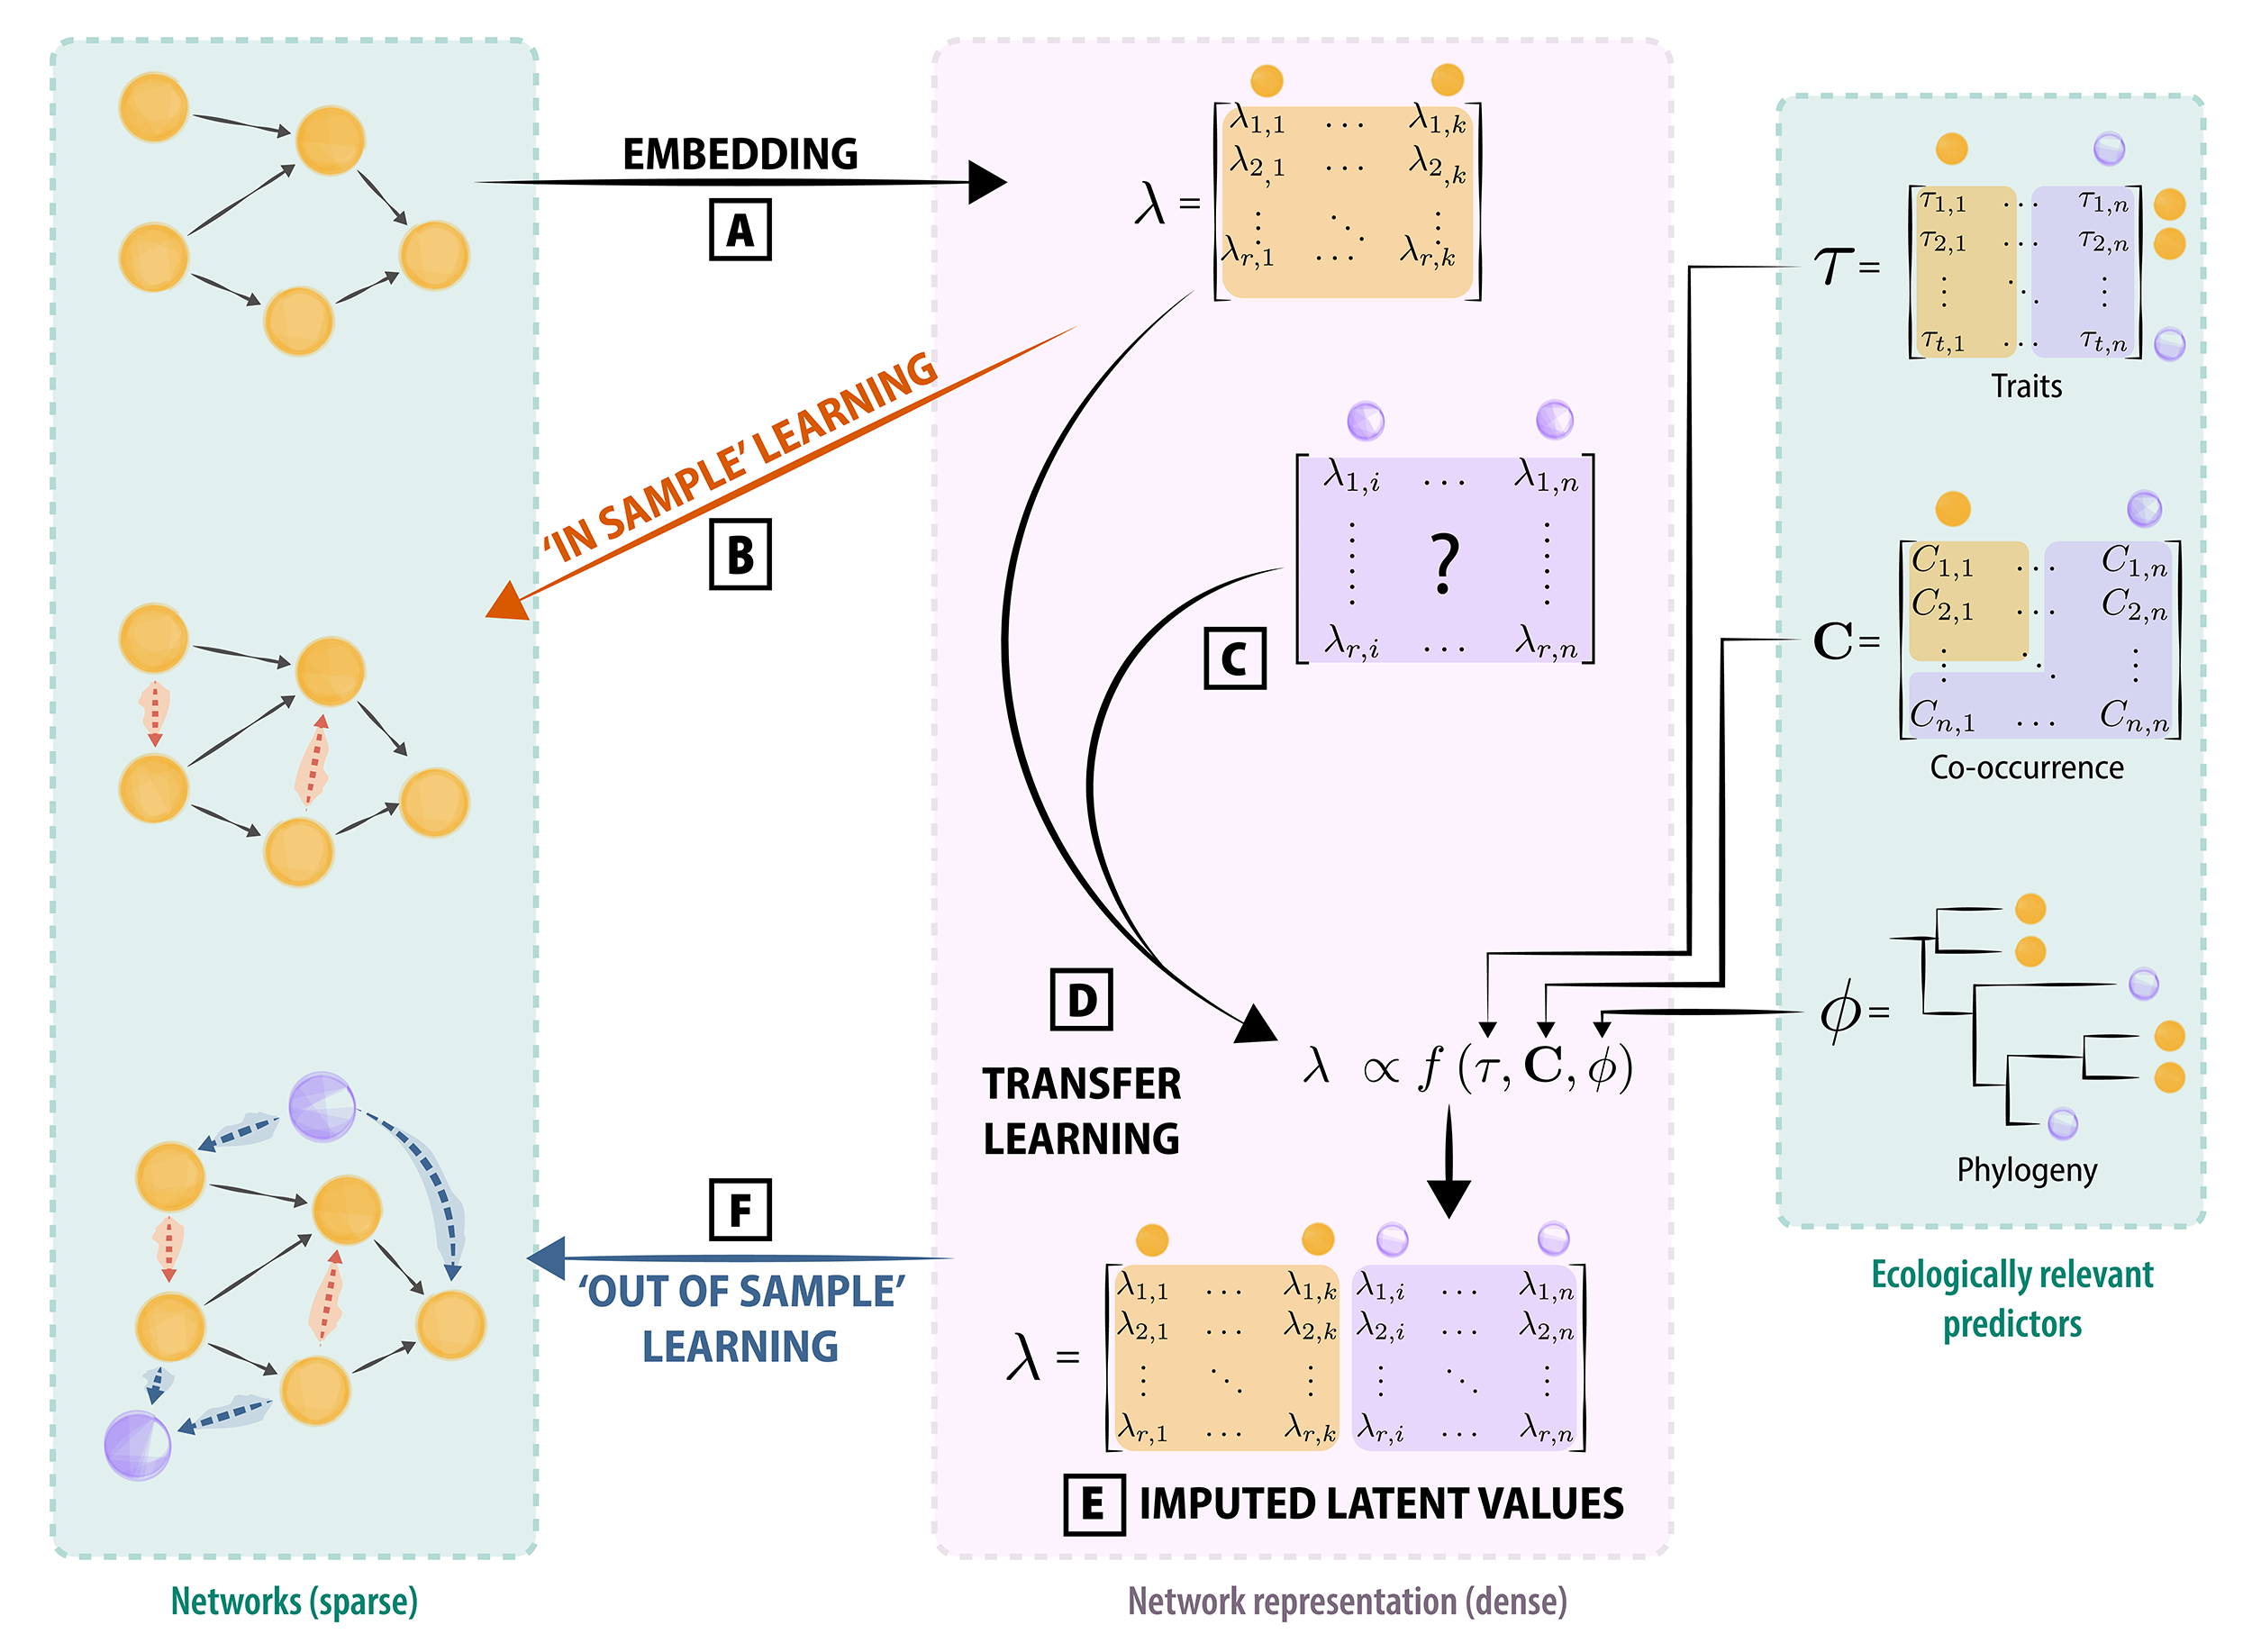
\includegraphics[width=\textwidth]{figures/conceptual_2.png}
    \caption{The embedding process (\textbf{A}) can help to identify links
(interactions) that may have been missed within the original community
(represented by the orange dashed arrows, \textbf{B}). Transfer learning
(\textbf{D}) allows for the prediction links (interactions) even when
novel species (\textbf{C}) are included alongside the original
community. This is achieved by learning using other relevant predictors
(\emph{e.g.,} traits) in conjunction with the known interactions to infer
latent values (\textbf{E}). Ultimately this allows us to predict links
(interactions) for species external from the original sample (blue
dashed arrows) as well as missing within sample links (\textbf{F}).
Within this context the predicted (and original) networks as well as the
ecological predictors used (green boxes) are products that can be
quantified through measurements in the field, whereas the embedded as
well as imputed matrices (purple box) are representative of a
decomposition of the interaction matrices onto the embedding
space}
    \label{fig:embedding}
\end{figure}

\section{Graph embedding offers promises for the inference of potential
interactions}\label{graph-embedding-offers-promises-for-the-inference-of-potential-interactions}

Graph (or network) embedding (\autoref{fig:embedding}) is a family of machine
learning techniques, whose main task is to learn a mapping function from
a discrete graph to a continuous domain (\cite{Arsov2019Network,
Chami2022Machine}). Their main goal is to learn a low dimensional
vector representation of the graph (embeddings), such that its key
properties (\emph{e.g.,} local or global structures) are retained in the
embedding space (\cite{Yan2005Graph}). The embedding space may, but will
not necessarily, have lower dimensionality than the graph. Ecological
networks are promising candidates for the routine application of
embeddings, as they tend to possess a shared structural backbone (see
\emph{e.g.,} \cite{BramonMora2018Identifying}), which hints at structural
invariants in empirical data. Assuming that these structural invariants
are common enough, they would dominate the structure of networks, and
therefore be adequately captured by the first (lower) dimensions of an
embedding, without the need to measure derived aspects of their
structure (\emph{e.g.,} motifs, paths, modularity, \ldots).

\subsection{Graph embedding produces latent variables (but not
traits)}\label{graph-embedding-produces-latent-variables-but-not-traits}

Before moving further, it is important to clarify the epistemic status
of node values derived from embeddings: specifically, they are
\emph{not} functional traits, and therefore should not be interpreted in
terms of effects or responses. As per the framework of
\cite{Malaterre2019Functional}, these values neither derive from, nor result
in, changes in organismal performance, and should therefore not be used
to quantify \emph{e.g.,} functional diversity. This holds true even when
there are correlations between latent values and functional traits:
although these enable an ecological discussion of how traits condition
the structure of the network, the existence of a statistical
relationship does not elevate the latent values to the status of
functional traits.

Rather than directly predicting biological rules (see \emph{e.g.,}
\cite{Pichler2020Machine} for an overview), which may be confounded by the
sparse nature of graph data, learning embeddings works in the
low-dimensional space that maximizes information about the network
structure. This approach is further justified by the observation, for
example, that the macro-evolutionary history of a network is adequately
represented by some graph embeddings (Random dot product graphs
(RDPG); see \cite{DallaRiva2016Exploring}). In a recent publication,
\cite{Strydom2022Food} have used an embedding (based on RDPG) to project a
metaweb of trophic interactions between European mammals, and
transferred this information to mammals of Canada, using the
phylogenetic distance between related clades to infer the values in the
latent subspace into which the European metaweb was projected. By
performing the RDPG step on re-constructed values, this approach yields
a probabilistic trophic metaweb for mammals of Canada based on knowledge
of European species, despite a limited (\(\approx\) 5\%) taxonomic
overlap, and illustrates how the values derived from an embedding can be
used for prediction without being ``traits'' of the species they
represent.

\subsection{Ecological networks are good candidates for
embedding}\label{ecological-networks-are-good-candidates-for-embedding}

Food webs are inherently low-dimensional objects, and can be adequately
represented with less than ten dimensions (\cite{Braga2021Phylogenetic,
Eklof2013Dimensionality, Braga2019Spatial}). Simulation results by
\cite{Botella2022Appraisal} suggested that there is no dominant method to
identify architectural similarities between networks: multiple
approaches need to be tested and compared to the network descriptor of
interest on a problem-specific basis. This matches previous results on
graph embedding, wherein different embedding algorithms yield different
network embeddings (\cite{Goyal2018Graph}), calling for a careful
selection of the problem-specific approach to use. In \autoref{tbl:methods}, we
present a selection of common graph and node embedding methods,
alongside examples of their use to predict interactions or statistical
associations between species. These methods rely largely on linear
algebra or pseudo-random walks on graphs. All forms of embeddings
presented in \autoref{tbl:methods} share the common property of summarizing their
objects into (sets of) dense feature vectors, that capture the overall
network structure, pairwise information on nodes, and emergent aspects
of the network, in a compressed way (\emph{i.e.,} with some information
loss, as we later discuss in the illustration). Node embeddings tend to
focus on maintaining pairwise relationships (\emph{i.e.,} species
interactions), while graph embeddings focus on maintaining the network
structure (\emph{i.e.,} emergent properties). Nevertheless, some graph
embedding techniques (like RDPG, see \emph{e.g.,} \cite{Wu2021Maximum}) will
provide high-quality node-level embeddings while also preserving network
structure.

Graph embeddings \emph{can} serve as a dimensionality reduction method.
For example, RDPG (\cite{Strydom2022Food}) and t-SVD (truncated Singular
Value Decomposition; (\cite{Poisot2021ImpMam}) typically embed networks
using fewer dimensions than the original network (the original network
has as many dimensions as species, and as many informative dimensions as
trophically unique species; \cite{Strydom2021SvdEnt}). However, this is not
necessarily the case -- indeed, one may perform a PCA (a special case of
SVD) to project the raw data into a subspace that improves the efficacy
of t-SNE (t-distributed stochastic neighbor embedding;
\cite{Maaten2009Learning}). There are many dimensionality reductions
(\cite{Anowar2021Conceptual}) that can be applied to an embedded network
should the need for dimensionality reduction (for example for data
visualization) arise. In brief, many graph embeddings \emph{can} serve
as dimensionality reduction steps, but not all do, neither do all
dimensionality reduction methods provide adequate graph embedding
capacities. In the next section (and \autoref{fig:embedding}), we show how the
amount of dimensionality reduction can affect the quality of the
embedding.

\begin{table}[h]
\resizebox{\textwidth}{!}{
\centering
\begin{tabular}{||c c c c c||} 
 \hline
 Method & Object & Technique & Reference & Application \\ [0.2ex] \hline\hline
 tSNE & nodes & statistical divergence & \cite{Hinton2002Stochastic} &
(\cite{Cieslak2020Tdistributed}, species-environment responses\(^a\)
\cite{Gibb2021Data},\newline host-virus network representation) \\
LINE & nodes & stochastic gradient descent & \cite{Tang2015Line} & \\
SDNE & nodes & gradient descent & \cite{Wang2016Structural} & \\
node2vec & nodes & stochastic gradient descent & \cite{Grover2016Node2vec}
& \\
HARP & nodes & meta-strategy & \cite{Chen2017Harp} & \\
DMSE & joint nodes & deep neural network & \cite{Chen2017Deep} &
\cite{Chen2017Deep}, species-environment interactions\(^b\) \\
graph2vec & sub-graph & skipgram network & \cite{Narayanan2017Graph2vec} & \\
RDPG & graph & SVD & \cite{Young2007Random} & \cite{DallaRiva2016Exploring},
trophic interactions \cite{Poisot2021ImpMam}, host-virus network
prediction \\
GLEE & graph & Laplacian eigenmap & \cite{Torres2020Glee} & \\
DeepWalk & graph & stochastic gradient descent & \cite{Perozzi2014Deepwalk} &
\cite{Wardeh2021Predicting}, host-virus interactions \\
GraphKKE & graph & stochastic differential equation &
\cite{Melnyk2020Graphkke} & \cite{Melnyk2020Graphkke}, microbiome species
associations\(^a\) \\
FastEmbed & graph & eigen decomposition & \cite{Ramasamy2015Compressive} & \\
PCA & graph & eigen decomposition & \cite{Surendran2013Graph} &
\cite{Strydom2021Roadmap}, host-parasite interactions) \\
Joint methods & multiple graphs & multiple strategies & \cite{Wang2021Joint}
& \\ [0.2ex]  
 \hline
\end{tabular}
}
\caption{Overview of some common graph embedding approaches, by type of
embedded objects, alongside examples of their use in the prediction of
species interactions. These methods have not yet been routinely used to
predict species interactions; most examples that we identified were
either statistical associations, or analogues to joint species
distribution models. See also Box 1 additional discussion on Graph Neural Networks. \(^a\): application is concerned with
\emph{statistical} interactions, which are not necessarily direct
biotic interactions; \(^b\):application is concerned with joint-SDM-like
approach, which is also very close to statistical associations as
opposed to direct biotic interactions. Given the need to evaluate
different methods on a problem-specific basis, the fact that a lot of
methods have not been used on network problems is an opportunity for
benchmarking and method development. Note that the row for PCA also
applies to kernel/probabilistic PCA, which are variations on the more
general method of SVD. Note further that tSNE has been included because
it is frequently used to embed graphs, including of species
associations/interactions, despite not being strictly speaking, a graph
embedding technique (see \emph{e.g.,} \cite{Chami2022Machine}.)}
\label{tbl:methods}
\end{table}

\clearpage

\begin{summary}
\textbf{Graph Neural Networks}

One prominent family of approaches we do not discuss in the present
manuscript is Graph Neural Networks (GNN; \cite{Zhou2020Graph}). GNN are,
in a sense, a method to embed a graph into a dense subspace, but belong
to the family of deep learning methods, which has its own set of
practices (see \emph{e.g.,} \cite{Goodfellow2016Deep}). An important issue with
methods based on deep learning is that, because their parameter space is
immense, the sample size of the data fed into them must be similarly
large (typically thousands of instances). This is a requirement for the
model to converge correctly during training, but this assumption is
unlikely to be met given the size of datasets currently available for
metawebs (or single time/location species interaction networks). This
data volume requirement is mostly absent from the techniques we list
below. Furthermore, GNN still have some challenges related to their
shallow structure, and concerns related to scalability (see
\cite{Gupta2021Graph} for a review), which are mostly absent from the
methods listed in \autoref{tbl:methods}. Assuming that the uptake of
next-generation biomonitoring techniques does indeed deliver larger
datasets on species interactions (\cite{Bohan2017Nextgeneration}), there
is nevertheless the potential for GNN to become an applicable
embedding/predictive technique in the coming years.
\end{summary}

The popularity of graph embedding techniques in machine learning is more
than the search for structural invariants: graphs are discrete objects,
and machine learning techniques tend to handle continuous data better.
Bringing a sparse graph into a continuous, dense vector space
(\cite{Xu2021Understanding}) opens up a broader variety of predictive
algorithms, notably of the sort that are able to predict events as
probabilities (\cite{Murphy2022Probabilistic}). Furthermore, the
projection of the graph itself is a representation that can be learned;
(\cite{Runghen2021Exploiting}), for example, used a neural network to learn the
embedding of a network in which not all interactions were known, based
on the nodes' metadata. This example has many parallels in ecology (see
\autoref{fig:embedding} \textbf{C}), in which node metadata can be represented by
phylogeny, abundance, or functional traits. Using phylogeny as a source
of information assumes (or strives to capture) the action of
evolutionary processes on network structure, which at least for food
webs have been well documented (\cite{Braga2021Phylogenetic,
DallaRiva2016Exploring, Eklof2016Phylogenetic, Stouffer2007Evidence,
Stouffer2012Evolutionary}); similarly, the use of functional traits
assumes that interactions can be inferred from the knowledge of
trait-matching rules, which is similarly well supported in the empirical
literature (\cite{Bartomeus2013Understanding, Bartomeus2016ComFra,
Goebel2023Body, Gravel2013Inferring}). Relating this information to
an embedding rather than a list of network measures would allow to
capture their effect on the more fundamental aspects of network
structure; conversely, the absence of a phylogenetic or functional
signal may suggest that evolutionary/trait processes are not strong
drivers of network structure, therefore opening a new way to perform
hypothesis testing.

\section{An illustration of metaweb
embedding}\label{an-illustration-of-metaweb-embedding}

In this section, we illustrate the embedding of a collection of
bipartite networks collected by \cite{Hadfield2014TalTwo}, using t-SVD and RDPG.
Briefly, an RDPG decomposes a network into two subspaces (left and
right), which are matrices that when multiplied give an approximation of
the original network. RDPG has the particularly desirable properties of
being a graph embedding technique that produces relevant node-level
feature vectors, and provides good approximations of graphs with varied
structures (\cite{Athreya2017Statistical}). The code to reproduce this
example is available as supplementary material in \autoref{supp:perspectives} (note, for the sake of
comparison, that \cite{Strydom2021Roadmap} have an example using embedding
through PCA followed by prediction using a deep neural network on the
same dataset). The resulting (binary) metaweb \(\mathcal{M}\) has 2131
interactions between 206 parasites and 121 hosts, and its adjacency
matrix has full rank (\emph{i.e.,} it represents a space with 121
dimensions). All analyses were done using \texttt{Julia} (\cite{Bezanson2017Julia})
version 1.7.2, \emph{Makie.jl} (\cite{Danisch2021Makie}), and
\emph{EcologicalNetworks.jl} (\cite{Poisot2019EcoJl}).

\begin{figure}[h]
    \centering
    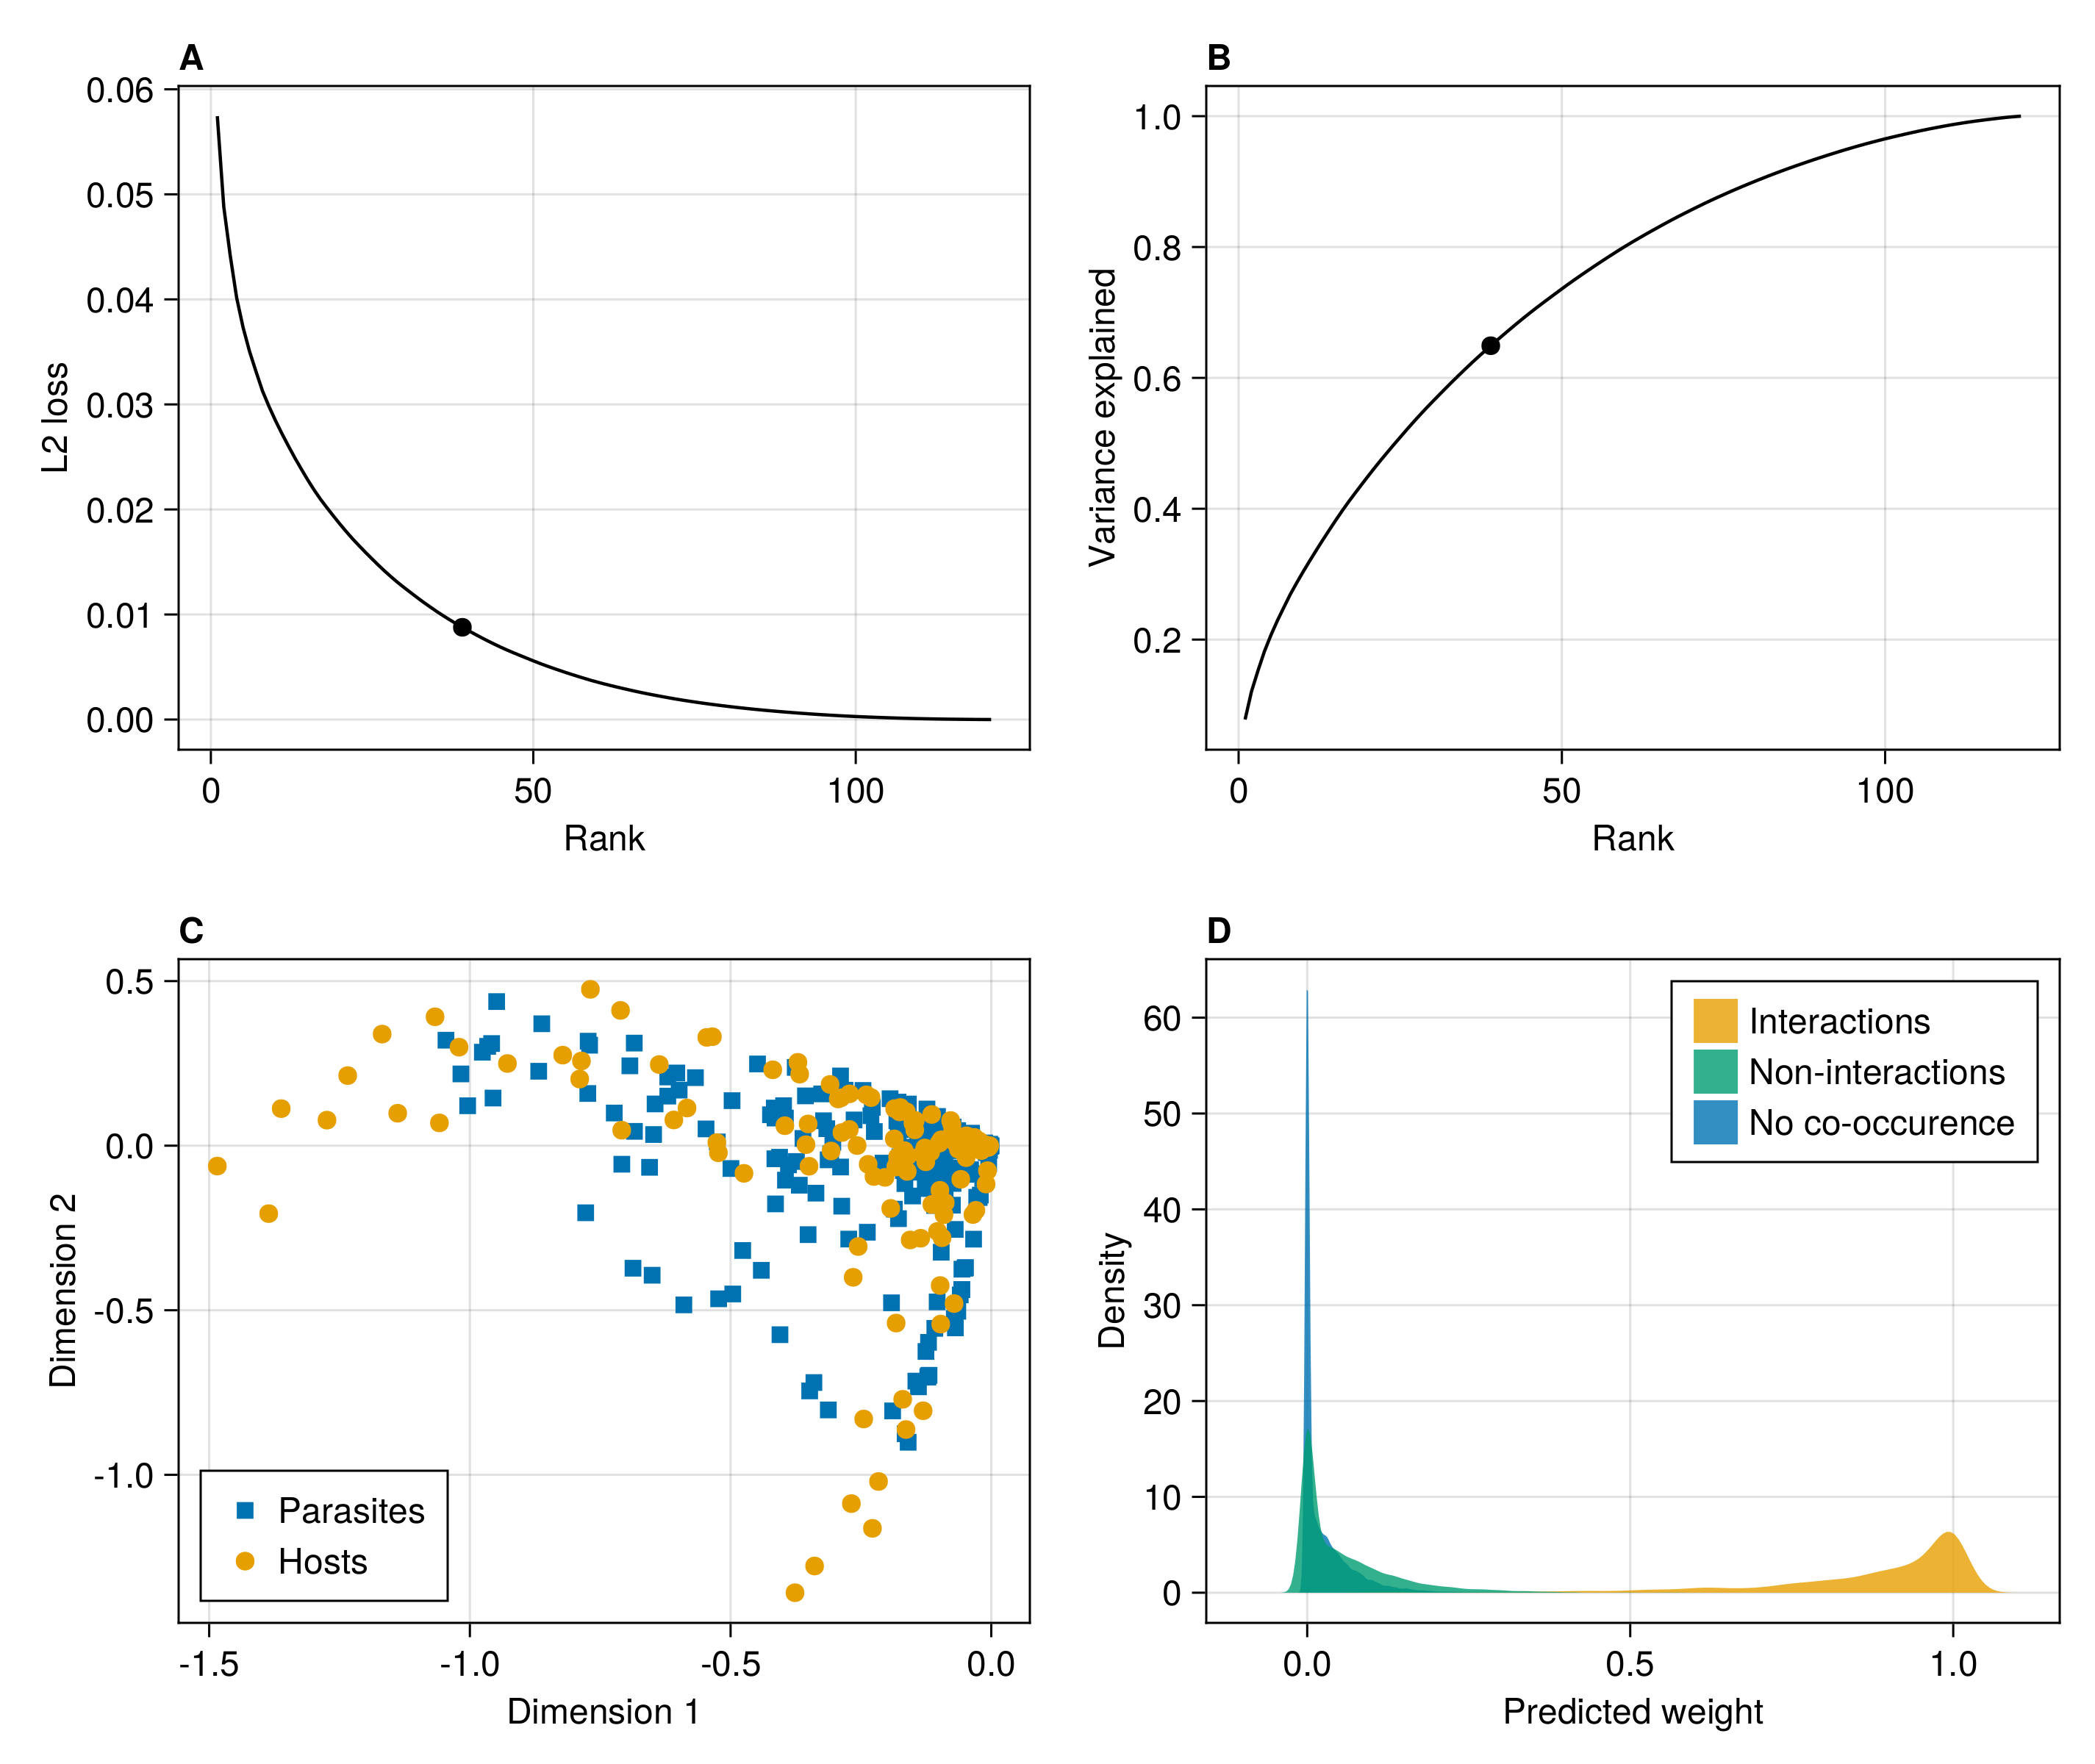
\includegraphics[width=\textwidth]{figures/illustration-part1.png}
    \caption{Validation of an embedding for a host-parasite metaweb, using
Random Dot Product Graphs. \textbf{A}, decrease in approximation error
as the number of dimensions in the subspaces increases. \textbf{B},
increase in cumulative variance explained as the number of ranks
considered increases; in \textbf{A} and \textbf{B}, the dot represents
the point of inflexion in the curve (at rank 39) estimated using the
finite differences method. \textbf{C}, position of hosts and parasites
in the space of latent variables on the first and second dimensions of
their respective subspaces (the results have been clamped to the unit
interval). \textbf{D}, predicted interaction weight from the RDPG based
on the status of the species pair in the
metaweb.}
    \label{fig:illustration1}
\end{figure}


In \autoref{fig:illustration1}, we focus on some statistical checks of the
embedding. In panel \textbf{A}, we show that the averaged \(L_2\) loss
(\emph{i.e.,} the sum of squared errors) between the empirical and
reconstructed metaweb decreases when the number of dimensions (rank) of
the subspace increases, with an inflection at 39 dimensions (out of 120
initially) according to the finite differences method. As discussed by
\cite{Runghen2021Exploiting}, there is often a trade-off between the number of
dimensions to use (more dimensions are more computationally demanding)
and the quality of the representation. In panel \textbf{B}, we show the
increase in cumulative variance explained at each rank, and visualize
that using 39 ranks explains about 70\% of the variance in the empirical
metaweb. This is a different information from the \(L_2\) loss (which is
averaged across interactions), as it works on the eigenvalues of the
embedding, and therefore captures higher-level features of the network.
In panel \textbf{C}, we show positions of hosts and parasites on the
first two dimensions of the left and right subspaces. Note that these
values largely skew negative, because the first dimensions capture the
coarse structure of the network: most pairs of species do not interact,
and therefore have negative values. Finally in panel \textbf{D}, we show
the predicted weight (\emph{i.e.,} the result of the multiplication of
the RDGP subspaces at a rank of 39) as a function of whether the
interactions are observed, not-observed, or unknown due to lack of
co-occurrence in the original dataset. This reveals that the observed
interactions have higher predicted weights, although there is some
overlap; the usual approach to identify potential interactions based on
this information would be a thresholding analysis, which is outside the
scope of this manuscript (and is done in the papers cited in this
illustration). Because the values returned from RDPG are not bound to
the unit interval, we performed a clamping of the weights to the unit
space, showing a one-inflation in documented interactions, and a
zero-inflation in other species pairs. This last figure crosses from the
statistical into the ecological, by showing that species pairs with no
documented co-occurrence have weights that are not distinguishable from
species pairs with no documented interactions, suggesting that (as
befits a host-parasite model) the ability to interact is a strong
predictor of co-occurrence.

\begin{figure}[h]
    \centering
    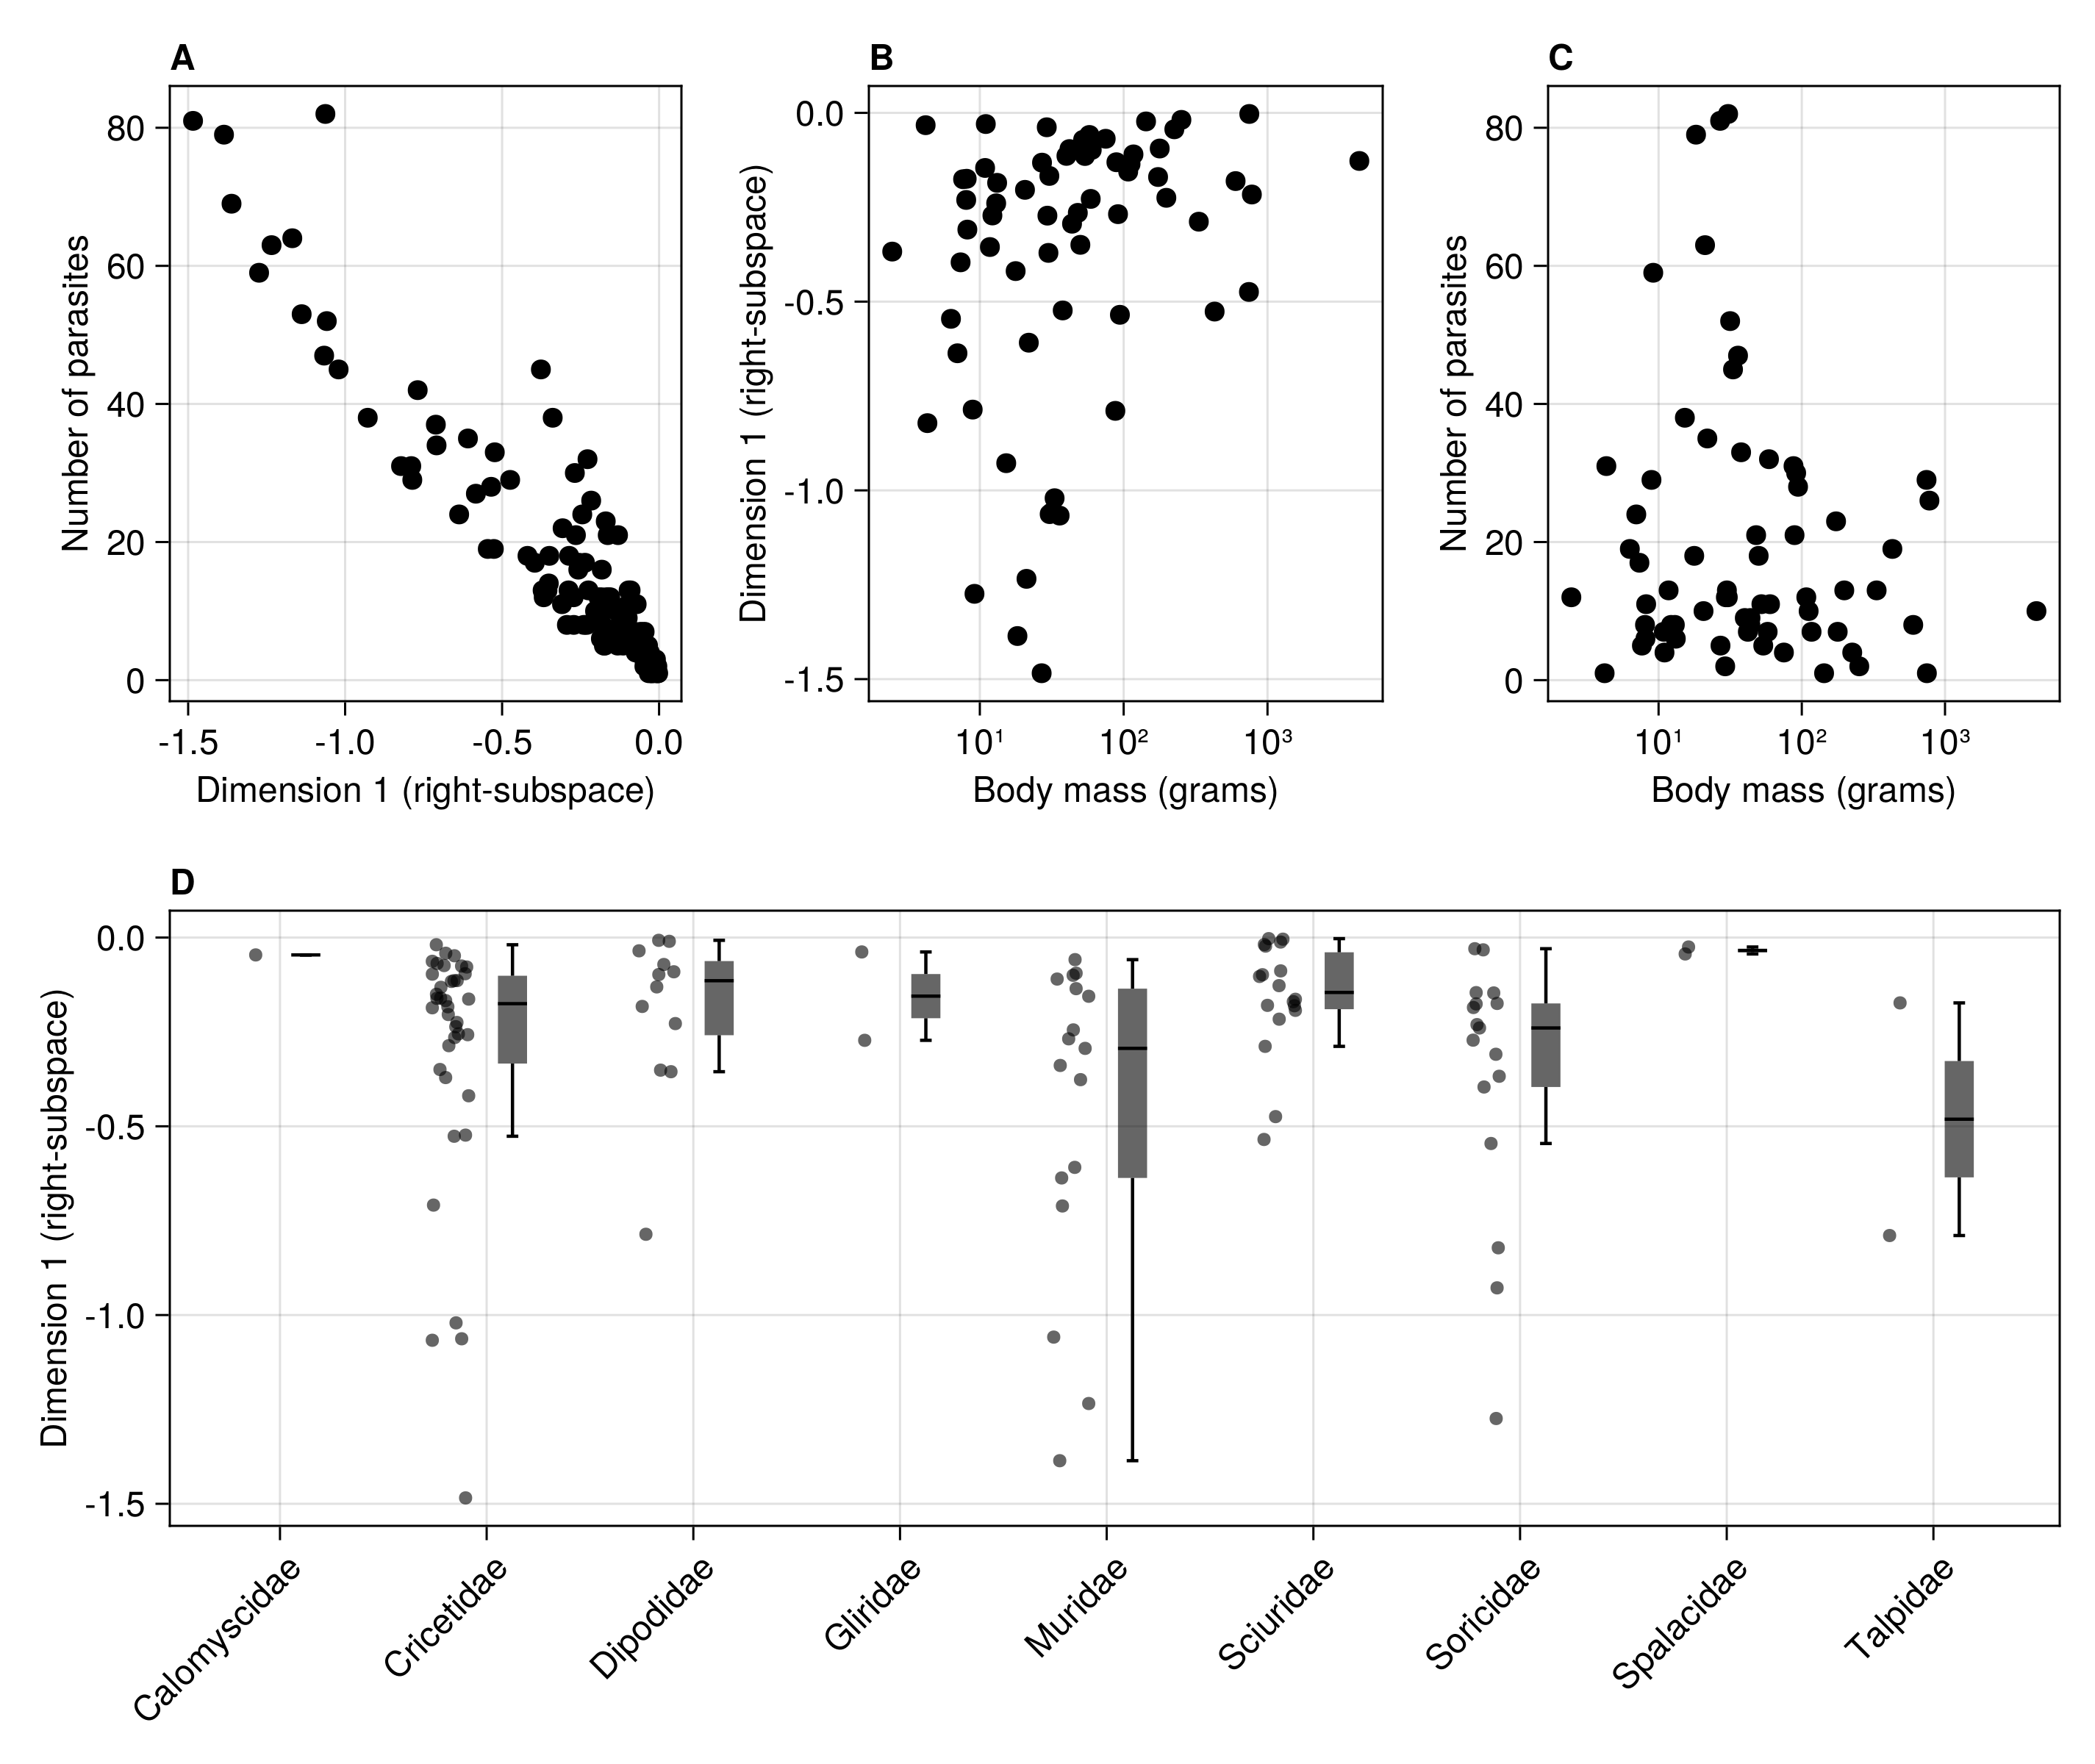
\includegraphics[width=\textwidth]{figures/illustration-part2.png}
    \caption{Ecological analysis of an embedding for a host-parasite
metaweb, using Random Dot Product Graphs. \textbf{A}, relationship
between the number of parasites and position along the first axis of the
right-subspace for all hosts, showing that the embedding captures
elements of network structure at the species scale. \textbf{B}, weak
relationship between the body mass of hosts (in grams) and the position
alongside the same dimension. \textbf{C}, weak relationship between body
mass of hosts and parasite richness. \textbf{D}, distribution of
positions alongside the same axis for hosts grouped by taxonomic
family.}
    \label{fig:illustration2}
\end{figure}

The results of \autoref{fig:illustration1} show that we can extract an embedding
of the metaweb that captures enough variance to be relevant;
specifically, this is true for both \(L_2\) loss (indicating that RDPG
is able to capture pairwise processes) and the cumulative variance
explained (indicating that RDPG is able to capture network-level
structure). Therefore, in \autoref{fig:illustration2}, we relate the values of
latent variables for hosts to different ecologically-relevant data. In
panel \textbf{A}, we show that host with a higher value on the first
dimension have fewer parasites. This relates to the body size of hosts
in the \emph{PanTHERIA} database (\cite{Jones2009Pantheria}), as shown in
panel \textbf{B}: interestingly, the position on the first axis is only
weakly correlated to body mass of the host; this matches well
established results showing that body size/mass is not always a direct
predictor of parasite richness in terrestrial mammals
(\cite{Morand1998Density}), a result we observe in panel \textbf{C}.
Finally, in panel \textbf{D}, we can see how different taxonomic
families occupy different positions on the first axis, with \emph{e.g.,}
Sciuridae being biased towards higher values. These results show how we
can look for ecological informations in the output of network
embeddings, which can further be refined into the selection of
predictors for transfer learning.

\section{The metaweb merges ecological hypotheses and
practices}\label{the-metaweb-merges-ecological-hypotheses-and-practices}

Metaweb inference seeks to provide information about the interactions
between species at a large spatial scale, typically a scale large enough
to be considered of biogeographic relevance (indeed, many of the
examples covered in the introduction span areas larger than a country,
some of them global). But as \cite{Herbert1965Dune} rightfully pointed out,
``[y]ou can't draw neat lines around planet-wide problems''; any
inference of a metaweb must therefore contend with several novel,
interwoven, families of problems. In this section, we outline three that
we think are particularly important, and can discuss how they may
addressed with subsequent data analysis or simulations, and how they
emerge in the specific context of using embeddings; some of these issues
are related to the application of these methods at the science-policy
interface.

\subsection{Identifying the properties of the network to
embed}\label{identifying-the-properties-of-the-network-to-embed}

If the initial metaweb is too narrow in scope, notably from a taxonomic
point of view, the chances of finding another area with enough related
species (through phylogenetic relatedness or similarity of functional
traits) to make a reliable inference decreases. This is because transfer
requires similarity (\autoref{fig:embedding}). A diagnostic for the lack of
similar species would likely be large confidence intervals during
estimation of the values in the low-rank space. In other words, the
representation of the original graph is difficult to transfer to the new
problem. Alternatively, if the initial metaweb is too large
(taxonomically), then the resulting embeddings would need to represent
interactions between taxonomic groups that are not present in the new
location. This would lead to a much higher variance in the starting
dataset, and to under-dispersion in the target dataset, resulting in the
potential under or over estimation of the strength of new predicted
interactions. \cite{Llewelyn2022Predicting} provided compelling evidence for
these situations by showing that, even at small spatial scales, the
transfer of information about interactions becomes more challenging when
areas rich with endemic species are considered. The lack of well
documented metawebs is currently preventing the development of more
concrete guidelines. The question of phylogenetic relatedness and
distribution is notably relevant if the metaweb is assembled in an area
with mostly endemic species (\emph{e.g.,} a system that has undergone
recent radiation or that has remained in isolation for a long period of
time might not have an analogous system with which to draw knowledge
from), and as with every predictive algorithm, there is room for the
application of our best ecological judgement. Because this problem
relates to distribution of species in the geographic or phylogenetic
space, it can certainly be approached through assessing the performance
of embedding transfer in simulated starting/target species pools.

\subsection{Identifying the scope of the prediction to
perform}\label{identifying-the-scope-of-the-prediction-to-perform}

The area for which we seek to predict the metaweb should determine the
species pool on which the embedding is performed. Metawebs can be
constructed by assigning interactions in a list of species within
specific regions. The upside of this approach is that information
relevant for the construction of this dataset is likely to exist, as
countries usually set conservation goals at the national level
(\cite{Buxton2021Key}), and as quantitative instruments are consequently
designed to work at these scales (\cite{Turak2017Using}); specific
strategies are often enacted at smaller scales, nested within a specific
country (\cite{Ray2021Biodiversity}). However, there is no guarantee that
these arbitrary boundaries are meaningful. In fact, we do not have a
satisfying answer to the question of ``where does an ecological network
stop?'', the answer to which would dictate the spatial span to
embed/predict. Recent results by \cite{Martins2022Global} suggested that
networks are shaped within eco-regions, with abrupt structural
transitions from an eco-region to the next. Should this trend hold
generally, this would provide an ecologically-relevant scale at which
metawebs can be downscaled and predicted. Other solutions could leverage
network-area relationships to identify areas in which networks are
structurally similar (see \emph{e.g.,} \cite{Fortin2021Network,
Galiana2018Spatial, Galiana2022Ecological}). Both of these solutions
require ample pre-existing information about the network in space.
Nevertheless, the inclusion of species for which we have data but that
are not in the right spatial extent \emph{may} improve the performance
of approaches based on embedding and transfer, \emph{if} they increase
the similarity between the target and destination network. This proposal
can specifically be evaluated by adding nodes to the network to embed,
and assessing the performance of predictive models (see \emph{e.g.,}
\cite{Llewelyn2022Predicting}).

\section{Conclusion: metawebs, predictions, and
people}\label{conclusion-metawebs-predictions-and-people}

Predictive approaches in ecology, regardless of the scale at which they
are deployed and the intent of their deployment, originate in the
framework that contributed to the ongoing biodiversity crisis
(\cite{Adam2014Elephant}) and reinforced environmental injustice
(\cite{Choudry2013Saving, Dominguez2020Decolonising}). The risk of
embedding this legacy in our models is real, especially when the impact
of this legacy on species pools is being increasingly documented. This
problem can be addressed by re-framing the way we interact with models,
especially when models are intended to support conservation actions.
Particularly on territories that were traditionally stewarded by
Indigenous people, we must interrogate how predictive approaches and the
biases that underpin them can be put to task in accompanying Indigenous
principles of land management (\cite{Eichhorn2019Steps,
Nokmaq2021Awakening}). The discussion of ``algorithm-in-the-loop''
approaches that is now pervasive in the machine learning community
provides examples of why this is important. Human-algorithm interactions
are notoriously difficult and can yield adverse effects
(\cite{Green2019Disparate, Stevenson2021Algorithmic}), suggesting the
need to systematically study them for the specific purpose of, here,
biodiversity governance. Improving the algorithmic literacy of decision
makers is part of the solution (\emph{e.g.,} \cite{Lamba2019Deep, 
MoseboFernandes2020Machine}), as we can reasonably expect that model
outputs will be increasingly used to drive policy decisions
(\cite{Weiskopf2022Increasing}). Our discussion of these approaches need
to go beyond the technical and statistical, and into the governance
consequences they can have. To embed data also embeds historical and
contemporary biases that acted on these data, both because they shaped
the ecological processes generating them, and the global processes
leading to their measurement and publication. For a domain as vast as
species interaction networks, these biases exist at multiple scales
along the way, and a challenge for prediction is not only to develop (or
adopt) new quantitative tools, but to assess the behavior of these tools
in the proper context.

\begin{summary}\label{box:people}
\textbf{Minding legacies shaping ecological datasets}

In large parts of the world, boundaries that delineate geographic
regions are merely a reflection the legacy of settler colonialism, which
drives global disparity in capacity to collect and publish ecological
data. Applying any embedding to biased data does not debias them, but
rather embeds these biases, propagating them to the models using
embeddings to make predictions. Furthermore, the use of ecological data
itself is not an apolitical act (\cite{Nost2021Political}): data
infrastructures tend to be designed to answer questions within national
boundaries (therefore placing contingencies on what is available to be
embedded), their use often drawing upon, and reinforcing, territorial
statecraft (see \emph{e.g.,} \cite{Barrett2005Environment}). As per
\cite{Machen2021Thinking}, these biases are particularly important to consider
when knowledge generated algorithmically is used to supplement or
replace human decision-making, especially for governance (\emph{e.g.,}
enacting conservation decisions on the basis of model prediction). As
information on networks is increasingly leveraged for conservation
actions (see \emph{e.g.,} \cite{Eero2021Use, Naman2022Food,
Stier2017Integrating}), the need to appraise and correct biases that
are unwittingly propagated to algorithms when embedded from the original
data is immense. These considerations are even more urgent in the
specific context of biodiversity data. Long-term colonial legacies still
shape taxonomic composition to this day (\cite{Lenzner2022Naturalized,
Raja2022Colonialism}), and much shorter-term changes in taxonomic and
genetic richness of wildlife emerged through environmental racism
(\cite{Schmidt2022Systemic}). Thus, the set of species found at a specific
location is not only as the result of a response to ecological processes
separate from human influence, but also the result of human-environment
interaction as well as the result legislative/political histories.
\end{summary}

\textbf{Acknowledgements:} We acknowledge that this study was conducted
on land within the traditional unceded territory of the Saint Lawrence
Iroquoian, Anishinabewaki, Mohawk, Huron-Wendat, and Omàmiwininiwak
nations. TP, TS, DC, and LP received funding from the Canadian Institute
for Ecology \& Evolution. FB is funded by the Institute for Data
Valorization (IVADO). TS, SB, and TP are funded by a donation from the
Courtois Foundation. CB was awarded a Mitacs Elevate Fellowship no.
IT12391, in partnership with fRI Research, and also acknowledges funding
from Alberta Innovates and the Forest Resources Improvement Association
of Alberta. M-JF acknowledges funding from NSERC Discovery Grant and
NSERC CRC. RR is funded by New Zealand's Biological Heritage Ngā Koiora
Tuku Iho National Science Challenge, administered by New Zealand
Ministry of Business, Innovation, and Employment. BM is funded by the
NSERC Alexander Graham Bell Canada Graduate Scholarship and the FRQNT
master's scholarship. LP acknowledges funding from NSERC Discovery Grant
(NSERC RGPIN-2019-05771). TP acknowledges financial support from the
Fondation Courtois, and NSERC through the Discovery Grants and Discovery
Accelerator Supplement programs. MJF is supported by an NSERC PDF and an
RBC Post-Doctoral Fellowship.


\printbibliography{}
\end{refsection}

\endinput
%%
%% End of file `article1.tex'.

%%
%% This is file `article1.tex', % generated with the docstrip utility.
%%
%% The original source files were:
%%
%% dms.dtx  (with options: `article') % Example TeX file for the documentation %
%of the jurabib package % Copyright (C) 1999, 2000, 2001 Jens Berger % See
%dms.ins  for the copyright details.
%% 
%%% ====================================================================
%%%  @LaTeX-file{ %%     filename        = "dms.dtx", %%     author    =
%"Nicolas Beauchemin, Damien Rioux-Lavoie, Victor Fardel, Jonathan Godin", %%
%copyright = "Copyright (C) 2000 , DMS %%                  all rights reserved.
%Copying of this file is %%                  authorized only if either: %%
%(1) you make absolutely no changes to your copy, %%                  including
%name; OR %%                  (2) if you do make changes, you first rename it %%
%to some other name.", %%     address   = "Département de Mathématiques et de
%Statistique", %%     telephone = "514-343-6705", %%     FAX       =
%"514-343-5700", %%     email     = "aide@dms.umontreal.ca (Internet)", %%
%keywords  = "latex, amslatex, ams-latex, theorem", %%     abstract  = " Ce
%fichier est un package conçu pour être %%                  utilisé avec la
%version de LaTeX2e 1995/06/01. Il %%                  est prévue pour la classe
%``amsbook''. Il en %%                  modifie le format des pages, l'entête
%des %%                  sections, etc, afin d'être  conforme au modèle de %%
%mémoire de maîtrise de l'Université de %%                  Montréal. Finalement
%ce fichier est grandement %%                  inspiré du fichier
%amsclass.dtx.", %%     docstring = "The checksum field contains: CRC-16
%checksum, %%                  word count, line count, and character count, as
%%%                  produced by Robert Solovay's checksum utility."}
%%%  ====================================================================


%% To change chapter header dynamically from french to english, use
%%\entetedynamique
\setcounter{corA}{0} % Pour recommancer à compter les def,
                     % theo, etc. à partir de 1
 % Pour écrire un article en français
%% \francais
 % Pour écrire un article en anglais
\anglais
%% NOTE: La plupart des macros ont un nom en anglais. % P.ex. \adresse et
%\address fonctionnent et sont équivalents. % \revue=\journal % \auteur=\author
%% \titre=\title

\doublespacing

%% Les contributions apparaîtront habituellement après % \maketitle (voir un peu
%plus bas). Selon les goûts, il est % possible de mettre les contributions %
%avant la page titre de l'article, simplement en les écrivant % directement ici.
%Par exemple :
 % \cleardoublepage \pdfbookmark[chapter]{Contributions}{contrib1} % Remplacer
 % par contrib2 pour l'article 2 etc. {\bfseries\Large\noindent Contributions de
 % <mon nom> et rôle joué par les coauteurs} J'ai contribué en...
 %
 % Le rôle des coauteurs a été de...

%% Nom de la revue de publication
\revue{Methods in Ecology and Evolution and can be found at https://doi.org/10. 1111/2041-210X.13835}
\article{Food web reconstruction through phylogenetic transfer of low-rank network representation}\label{Foodweb}
%% On peut se référer aux numéros de chapitre ou d'article comme suit. % Si on
%fait % \label{chap:article1}, % alors \ref{chap:article1} donnera le numéro du
%chapitre. On peut ensuite faire % \labelart{art:article1} % et alors
%\ref{art:article1} donnera le numéro d'article. % Par exemple, si cette article
%est le premier article et le deuxième chapitre, % alors si on écrit % Voir le
%chapitre~\ref{chap:article1} (l'article~\ref{art:article1}). % deviendra % Voir
%le chapitre 2 (l'article 1). % Si on veut écrire « premier article » au lieu «
%article 1 », on peut % simplement faire % \ordinal{\ref{art:article1}}~article
%% devient première article % ou % \Ordinal{\ref{art:article1}}~article  %
%devient Première article (avec la majuscule) % Si on est en mode \anglais,
%\ordinal écrire first, second,...

%%%%%%%%%%%%%%%%%%%%%%%%%%%%%%%%%%%%%%%%%%%%%%%%%%%%%%%%%%%%%%%
%%%%%%%%%%%%%%%%%     Contribution     %%%%%%%%%%%%%%%%%%%%%%%% %%%%%%%%%%%%%%%%
%(lire attentivement) %%%%%%%%%%%%%%%%%%%%%%%%
%%%%%%%%%%%%%%%%%%%%%%%%%%%%%%%%%%%%%%%%%%%%%%%%%%%%%%%%%%%%%%%
 % Contribution(s) peronnelle(s) à l'article et rôle joué par tous les
 % coauteur·e·s
 %
 % Nécessaire seulement lorsque vous n'êtes pas seul·e auteur·e. Les
 % contributions peuvent apparaître ailleur dans la thèse. Si \contributions est
 % laissé vide (p.ex. si vous effacez celui ci-bas), aucune contributions ne
 % seront générées sur la page titre de l'article. Vous pouvez alors mettre un
 % \newpage si vous souhaitez que les résumé et abstract soient sur la page
 % suivante.
 %
 % REMARQUE : À peu près toutes les constructions \LaTeX\ sont permises dans les
 % contributions.
 %
 % La commande admet une option [<entête>]
\contributions%[Mes contributions et le rôle des coauteurs]
{ T.S., S.B. and T.P. designed the study and performed the analysis; G.V.D.R., M.J.F. and R.R. provided additional feedback on the analyses; D.C., B.M. and F.B. helped with data collection. All authors contributed to writing and editing the manuscript. \\[1cm]
}

%%% INFORMATIONS POUR LA PAGE TITRE
 % Premier auteur·e et adresse

\auteur{Tanya Strydom}
\adresse{Département de Sciences Biologiques, Université de Montréal, Montreal, QC, Canada\\ Québec Centre for Biodiversity Sciences, Montreal, QC, Canada}
\auteur{Salomé Bouskila}
\adresse{Département de Sciences Biologiques, Université de Montréal, Montreal, QC, Canada\\ Québec Centre for Biodiversity Sciences, Montreal, QC, Canada}
\auteur{Francis Banville}
\adresse{Département de Sciences Biologiques, Université de Montréal, Montreal, QC, Canada\\
Université de Sherbrooke, Sherbrooke, Canada\\
Québec Centre for Biodiversity Sciences, Montreal, QC, Canada}
\auteur{Ceres Barros}
\adresse{Department of Forest Resources Management, University of British Columbia, Vancouver, BC, Canada}
\auteur{Dominique Caron}
\adresse{McGill University, Montréal, Canada\\ Québec Centre for Biodiversity Sciences, Montreal, QC, Canada}
\auteur{Maxwell J. Farrell}
\adresse{Department of Ecology \& Evolutionary Biology, University of Toronto, Toronto, ON, Canada}
\auteur{Marie-Josée Fortin}
\adresse{Department of Ecology \& Evolutionary Biology, University of Toronto, Toronto, ON, Canada}
\auteur{Victoria Hemming}
\adresse{Department of Forest and Conservation Sciences, University of British Columbia, Vancouver, BC, Canada}
\auteur{Benjamin Mercier}
\adresse{Université de Sherbrooke, Sherbrooke, Canada\\
Québec Centre for Biodiversity Sciences, Montreal, QC, Canada}
\auteur{Laura Pollock}
\adresse{McGill University, Montréal, Canada\\ Québec Centre for Biodiversity Sciences, Montreal, QC, Canada}
\auteur{Rogini Runghen}
\adresse{Centre for Integrative Ecology, School of Biological Sciences, University of Canterbury, Canterbury, New Zealand}
\auteur{Giulio V. Dalla Riva}
\adresse{School of Mathematics and Statistics, University of Canterbury, Christchurch, New Zealand}
\auteur{Timothée Poisot}
\adresse{Département de Sciences Biologiques, Université de Montréal, Montreal, QC, Canada\\ Québec Centre for Biodiversity Sciences, Montreal, QC, Canada}
%

\maketitle

\begin{resume}{estimation des caractères ancestraux, biogéographie, réseaux écologiques, intégration de réseaux, apprentissage par transfert} 1. Malgré leur importance dans de nombreux processus écologiques, la collecte de données et d’informations sur les interactions écologiques est une tâche extrêmement complexe. Pour cette raison, de nombreuses régions du monde révèlent un déficit de données en ce qui concerne les interactions entre les espèces et la structure des réseaux qui en résultent. Comme il est peu probable que la collecte de données soit suffisante à elle seule, les écologistes des communautés doivent adopter des méthodes prédictives.\\
2. Nous présentons un cadre méthodologique qui utilise l’incorporation graphique et l’apprentissage par transfert pour établir une liste prédictive des interactions trophiques d’un bassin d’espèces dont les interactions sont inconnues. Plus précisément, nous « apprenons » l’information (caractères latents) des espèces à partir d’un réseau d’interaction connu et inférons les caractères latents d’un autre bassin d’espèces pour lequel nous n’avons pas de données d’interaction a priori fondées sur leur lien phylogénétique avec les espèces du réseau connu. Les traits latents peuvent ensuite être utilisés pour prédire les interactions et construire un réseau d’interaction.\\
3. Ici, nous avons assemblé un méta-réseau (metaweb) pour les mammifères canadiens à partir des interactions dans le réseau trophique européen, en dépit d’un partage d’espèces communes de seulement 4\% entre les deux sites. Les résultats du modèle prédictif sont comparés aux bases de données répertoriées d’interactions par paires, montrant que nous recouvrons correctement 91\% des interactions connues.\\
4. Le cadre est intrinsèquement robuste, même lorsque le réseau connu est incomplet ou contient des interactions fallacieuses, en faisant un candidat idéal comme outil pour combler les lacunes en ce qui concerne les interactions entre les espèces. Nous fournissons des conseils sur la façon dont ce cadre peut être adapté en remplaçant certaines approches ou certains prédicteurs afin de le rendre plus généralement applicable.\\
\end{resume}

\begin{abstract}{ancestral character estimation, biogeography, ecological networks, network embedding, transfer learning} 1. Despite their importance in many ecological processes, collecting data and information on ecological interactions is an exceedingly challenging task. For this reason, large parts of the world have a data deficit when it comes to species interactions and how the resulting networks are structured. As data collection alone is unlikely to be sufficient, community ecologists must adopt predictive methods.\\
2. We present a methodological framework that uses graph embedding and transfer learning to assemble a predicted list of trophic interactions of a species pool for which their interactions are unknown. Specifically, we ‘learn’ the information (latent traits) of species from a known interaction network and infer the latent traits of another species pool for which we have no \emph{a priori} interaction data based on their phylogenetic relatedness to species from the known network. The latent traits can then be used to predict interactions and construct an interaction network.\\
3. Here we assembled a metaweb for Canadian mammals derived from interactions in the European food web, despite only 4\% of common species being shared between the two locations. The results of the predictive model are compared against databases of recorded pairwise interactions, showing that we correctly recover 91\% of known interactions.\\
4. The framework itself is robust even when the known network is incomplete or contains spurious interactions making it an ideal candidate as a tool for filling gaps when it comes to species interactions. We provide guidance on how this framework can be adapted by substituting some approaches or predictors in order to make it more generally applicable.
\end{abstract}

\begin{refsection}

\section{Introduction}

There are two core challenges we are faced with in furthering our
understanding of ecological networks across space, particularly at
macro-ecologically relevant scales (\emph{e.g.,} \cite{Trojelsgaard2016EcoNet}).
First, ecological networks within a location are difficult to sample
properly (\cite{Jordano2016ChaEco, Jordano2016SamNet}), resulting in a
widespread ``Eltonian shortfall'' (\cite{Hortal2015Seven}), \emph{i.e.,} a
lack of knowledge about inter- and intra- specific relationships. This
first challenge has been, in large part, addressed by the recent
emergence of a suite of methods aiming to predict interactions within
\emph{existing} networks, many of which are reviewed in
(\cite{Strydom2021Roadmap}). Second, recent analyses based on collected data
(\cite{Poisot2021GloKno}) or metadata (\cite{Cameron2019Uneven}) highlight
that ecological networks are currently studied in a biased subset of
space and bioclimates, which impedes our ability to generalize any local
understanding of network structure. Meaning that, although the framework
to address incompleteness \emph{within} networks exists, there would
still be regions for which, due to a \emph{lack} of local interaction
data, we are unable to infer potential species interactions.

Here, we present a general method to infer potential trophic
interactions, relying on the transfer learning of network
representations, specifically by using similarities of species in a
biologically/ecologically relevant proxy space (\emph{e.g.,} shared
morphology or ancestry). Transfer learning is a machine learning
methodology that uses the knowledge gained from solving one problem and
applying it to a related (destination) problem (\cite{Torrey2010Transfer,
Pan2010Survey}). In this instance, we solve the problem of predicting
trophic interactions between species, based on knowledge extracted from
another species pool for which interactions are known by using
phylogenetic structure as a medium for transfer. There is a plurality of
measures of species similarities that can be used for inferring
\emph{potential} species interactions \emph{i.e.,} metaweb reconstruction
(see \emph{e.g.,} \cite{Morales-Castilla2015Inferring}); however, phylogenetic
proximity has several desirable properties when working at large scales.
\cite{Gerhold2015Phylogenetic} made the point that phylogenetic signal captures
diversification of characters (large macro-evolutionary process), but
not necessarily community assembly (fine ecological process);
\cite{Dormann2010Evolution} previously found very similar conclusions.
Interactions tend to reflect a phylogenetic signal because they have a
conserved pattern of evolutionary convergence that encompasses a wide
range of ecological and evolutionary mechanisms (\cite{Mouquet2012Ecophylogenetics, Cavender-Bares2009Merging}), and - most importantly - retain this
signal even if it is obscured at the community scale due to \emph{e.g.,}
local conditions (\cite{Poisot2018Interactions, Hutchinson2017Cophylogenetic}).
Finally, species interactions at macro-ecological scales seem to respond
mostly to macro-evolutionary processes (\cite{Price2003Macroevolutionary}); which is
evidenced by the presence of conserved backbones in food webs
(\cite{BramonMora2018Identifying, DallaRiva2016Exploring}), strong evolutionary
signature on prey choice (\cite{Stouffer2012Evolutionary}), and strong
phylogenetic signature in food web intervality (\cite{Eklof2016Phylogenetic}).
Phylogenetic reconstruction has also previously been used within the
context of ecological networks, namely understanding ancestral
plant-insect interactions (\cite{Braga2021Phylogenetic}). Taken together, these
considerations suggest that phylogenies can reliably be used to transfer
knowledge on species interactions.

\begin{figure}[h]
    \centering
    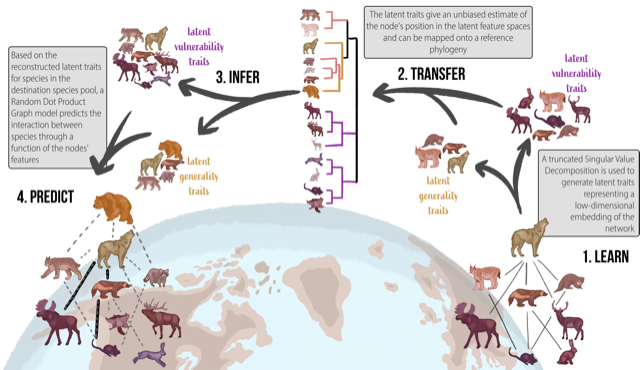
\includegraphics[width=\textwidth]{figures/figure-concept_v2.png}
    \caption{Overview of the phylogenetic transfer learning (and prediction)
of species interactions networks. Starting from an initial, known,
network, we learn its representation through a graph embedding step
(here, a truncated Singular Value Decomposition; Step 1), yielding a
series of latent traits (latent vulnerability traits are more
representative of species at the lower trophic-level and latent
generality traits are more representative of species at higher
trophic-levels; \emph{sensu} \cite{Schoener1989Food}); second, for the
destination species pool, we perform ancestral character estimation
using a phylogeny (here, using a Brownian model for the latent traits;
Step 2); we then sample from the reconstructed distribution of latent
traits (Step 3) to generate a probabilistic metaweb at the destination
(here, assuming a uniform distribution of traits), and threshold it to
yield the final list of interactions (Step 4).}
    \label{fig:concept}
\end{figure}

In \autoref{fig:concept}, we provide a methodological overview based on learning
the embedding of a metaweb of trophic interactions for European mammals
(known interactions; \cite{Maiorano2020Tetraeu, Maiorano2020Data}) and,
based on phylogenetic relationships between mammals globally \emph{i.e.,}
phylogenetic tree (\cite{Upham2019Inferring}), infer a metaweb for the Canadian
mammalian species pool (using only a species list \emph{i.e.,} we have no
prior data on species interaction data for Canada in this instance). Our
case study shows that phylogenetic transfer learning is an effective
approach to the generation of probabilistic metawebs. This showcases
that although the components (species) that make up the Canadian and
European communities may be \emph{minimally} shared (the overall species
overlap is less than 4\%), if the medium (proxy space) selected in the
transfer step is biologically plausible, we can still effectively learn
from the known network and make biologically relevant predictions of
interactions. Indeed, as we detail in the results, when validated
against the known (but fractional) data of trophic interactions present
between Canadian mammals, our model achieves a predictive accuracy of
approximately 91\%.

\section{Method description}\label{method-description}

The core point of our method is the transfer of knowledge of a known
ecological network to predict interactions between species for another
location for which the network is unknown (or partially known) and is
summarized in the grey text boxes in \autoref{fig:concept}. The method we develop
is, ecologically speaking, a ``black box'', \emph{i.e.,} an algorithm
that can be understood mathematically, but whose component parts are not
always directly tied to ecological processes. There is a growing
realization in machine learning that (unintentional) black box
algorithms are not necessarily a bad thing (\cite{Holm2019Defense}), as
long as their constituent parts can be examined (which is the case with
our method). But more importantly, data hold more information than we
might think; as such, even algorithms that are disconnected from a model
can make correct guesses most of the time (\cite{Halevy2009Unreasonable}); in
fact, in an instance of ecological forecasting of spatio-temporal
systems, model-free approaches (\emph{i.e.,} drawing all of their
information from the data) outperformed model-informed ones
(\cite{Perretti2013Modelfree}).

\subsection{Data used for the case
study}\label{data-used-for-the-case-study}

We use data from the European metaweb assembled by \cite{Maiorano2020Tetraeu}.
This was assembled using data extracted from scientific literature
(including published papers, books, and grey literature) from the last
50 years and includes all terrestrial tetrapods (mammals, breeding
birds, reptiles and amphibians) occurring on the European sub-continent
(and Turkey) - with the caveat that only species introduced in
historical times and currently naturalized being included. The European
metaweb was filtered using the Global Biodiversity Information Facility
(GBIF) taxonomic backbone (\cite{GBIFSecretariat2021Gbif}) so as to
contain only terrestrial and semi-aquatic mammals. As all species had
valid matches to the GBIF taxonomy it was used as the backbone for the
remaining reconciliation steps namely, the mammalian consensus supertree
by \cite{Upham2019Inferring} (which is used for the knowledge transfer step) and for the Canadian species list---which was extracted from the
International Union for Conservation of Nature (IUCN) checklist, and
corresponds to the same selection criteria that was applied by
\cite{Maiorano2020Tetraeu} in the European metaweb. After taxonomic cleaning
and reconciliation the European metaweb has 260 species, and the
Canadian species pool 163; of these, 17 (about 4\% of the total) are
shared, and 89 species from Canada (54\%) had at least one congeneric
species in Europe. The similarity for both species pools predictably
increases with higher taxonomic order, with 19\% of shared genera, 47\%
of shared families, and 75\% of shared orders; for the last point,
Canada and Europe each had a single unique order (\emph{Didelphimorphia}
for Canada, \emph{Erinaceomorpha} for Europe).

\subsection{Implementation and code
availability}\label{implementation-and-code-availability}

The entire pipeline is implemented in \texttt{Julia} 1.6
(\cite{Bezanson2017Julia}) and is available under the permissive MIT
License at \href{https://osf.io/2zwqm/}{\texttt{https://osf.io/2zwqm/}}.
The taxonomic cleanup steps are done using \texttt{GBIF.jl}
(\cite{Dansereau2021Simplesdmlayers}). The network embedding and analysis is done
using \texttt{EcologicalNetworks.jl} (\cite{Banville2021Mangal,,
Poisot2019EcoJl}). The phylogenetic simulations are done using
\texttt{PhyloNetworks.jl} (\cite{Solis-Lemus2017Phylonetworks}) and
\texttt{Phylo.jl} (\cite{Reeve2016How}). A complete
\texttt{Project.toml} file specifying the full tree of dependencies is
available alongside the code. This material also includes a fully
annotated copy of the entire code required to run this project
(describing both the intent of the code and discussing some technical
implementation details), a vignette for every step of the process, and a
series of Jupyter notebooks with the text and code. The pipeline can be
executed on a laptop in a matter of minutes, and therefore does not
require extensive computational power.

\subsection{Step 1: Learning the origin network
representation}\label{step-1-learning-the-origin-network-representation}

The first step in transfer learning is to learn the structure of the
original dataset. In order to do so, we rely on an approach inspired
from representational learning, where we learn a \emph{representation}
of the metaweb (in the form of the latent subspaces), rather than a list
of interactions (species \emph{a} eats \emph{b}). This approach is
conceptually different from other metaweb-scale predictions (\emph{e.g.,}
\cite{Albouy2019Marine}), in that the metaweb representation is easily
transferable. Specifically, we use a Random Dot Product Graph model
(hereafter RDPG; \cite{Young2007Random}) to create a number of latent
variables that can be combined into an approximation of the network
adjacency matrix. RDPG is known to capture the evolutionary backbone of
food webs (\cite{DallaRiva2016Exploring}), resulting in strong phylogenetic
signal in RDPG results; in other words, the latent variables of an RDPG
can be mapped onto a phylogenetic tree, and phylogenetically similar
predators should share phylogenetically similar preys. In addition,
recent advances show that the latent variables produced this way can be
used to predict \emph{de novo} interactions. Interestingly, the latent
variables do not need to be produced by decomposing the network itself;
in a recent contribution, (\cite{Runghen2021Exploiting}) showed that deep artificial
neural networks are able to reconstruct the left and right subspaces of
an RDPG, in order to predict human movement networks from
individual/location metadata and opens up the possibility of using
additional metadata as predictors.

The latent variables are created by performing a truncated Singular
Value Decomposition (t-SVD; \cite{Halko2011Finding}) on the adjacency
matrix. SVD is an appropriate embedding of ecological networks, which
has recently been shown to both capture their complex, emerging
properties (\cite{Strydom2021SvdEnt}) and to allow highly accurate
prediction of the interactions within a single network
(\cite{Poisot2021ImpMam}). Under SVD, an adjacency matrix \(\mathbf{A}\)
(where \(\mathbf{A}_{m,n}\in\mathbb{B}\) where 1 indicates predation and
0 an absence thereof) is decomposed into three components resulting in
\(\mathbf{A} = \mathbf{U}\mathbf{\Sigma}\mathbf{V'}.\) Here,
\(\mathbf{\Sigma}\) is a \(m \times n\) diagonal matrix and contains
only singular (\(\sigma\)) values along its diagonal, \(\mathbf{U}\) is
a \(m \times m\) unitary matrix, and \(\mathbf{V}'\) a \(n \times n\)
unitary matrix. Truncating the SVD removes additional noise in the
dataset by omitting non-zero and/or smaller \(\sigma\) values from
\(\mathbf{\Sigma}\) using the rank of the matrix. Under a t-SVD
\(\mathbf{A}_{m,n}\) is decomposed so that \(\mathbf{\Sigma}\) is a
square \(r \times r\) diagonal matrix (with \(1 \le r \le r_{full}\)
where \(r_{full}\) is the full rank of \(\mathbf{A}\) and \(r\) the rank
at which we truncate the matrix) containing only non-zero \(\sigma\)
values. Additionally, \(\mathbf{U}\) is now an \(m \times r\) semi
unitary matrix and \(\mathbf{V}'\) an \(r \times n\) semi-unitary
matrix.

The specific rank at which the SVD ought to be truncated is a difficult
question. The purpose of SVD is to remove the noise (expressed at high
dimensions) and to focus on the signal (expressed at low dimensions). In
datasets with a clear signal/noise demarcation, a scree plot of
\(\mathbf{\Sigma}\) can show a sharp drop at the rank where noise starts
(\cite{Zhu2006Automatic}). Because the European metaweb is almost entirely
known, the amount of noise (uncertainty) is low; this is reflected in
Fig.\ref{fig:scree} (left), where the scree plot shows no important drop, and in
Fig.\ref{fig:scree} (right) where the proportion of variance explained increases
smoothly at higher dimensions. For this reason, we default back to a
threshold that explains 60\% of the variance in the underlying data,
corresponding to 12 dimensions - \emph{i.e.,} a tradeoff between accuracy
and a reduced number of features.

An RDPG estimates the probability of observing interactions between
nodes (species) as a function of the nodes' latent variables, and is a
way to turn an SVD (which decompose one matrix into three) into two
matrices that can be multiplied to provide an approximation of the
network. The latent variables used for the RDPG, called the left and
right subspaces, are defined as
$\mathscr{L} = \mathbf{U}\sqrt{\mathbf{\Sigma}}$, and
$\mathscr{R} = \sqrt{\mathbf{\Sigma}}\mathbf{V}'$ -- using the full
rank of $\mathbf{A}, \mathscr{L}\mathscr{R} = \mathbf{A}$, and
using any smaller rank results in
$\mathscr{L}\mathscr{R} \approx \mathbf{A}$. Using a rank of 1 for the
t-SVD provides a first-order approximation of the network. One advantage
of using an RDPG for the network reconstruction rather than an SVD is
that the number of components to estimate decreases; notably, one does
not have to estimate the singular values of the SVD. Furthermore, the
two subspaces can be directly multiplied to yield a network.

\begin{figure}[h]
    \centering
    \includegraphics[width=\textwidth]{figures/figure-screeplot.png}
    \caption{Left: representation of the scree plot of the singular values
from the t-SVD on the European metaweb. The scree plot shows no obvious
drop in the singular values that may be leveraged to automatically
detect a minimal dimension for embedding, after \emph{e.g.,}
\cite{Zhu2006Automatic}. Right: cumulative fraction of variance explained by each
dimension up to the rank of the European metaweb. The grey lines
represent cutoffs at 50, 60, \ldots, 90\% of variance explained. For the
rest of the analysis, we reverted to an arbitrary threshold of 60\% of
variance explained, which represented a good tradeoff between accuracy
and reduced number of features.}
    \label{fig:scree}
\end{figure}

Because RDPG relies on matrix multiplication, the higher dimensions
essentially serve to make specific interactions converge towards 0 or 1;
therefore, for reasonably low ranks, there is no guarantee that the
values in the reconstructed network will be within the unit range. In
order to determine what constitutes an appropriate threshold for
probability, we performed the RDPG approach on the European metaweb, and
evaluated the probability threshold by treating this as a binary
classification problem, specifically assuming that both 0 and 1 in the
European metaweb are all true. Given the methodological details given in
\cite{Maiorano2020Tetraeu} and \cite{OConnor2020Unveiling}, this seems like a reasonable
assumption, although one that does not hold for all metawebs. We used
the thresholding approach presented in \cite{Poisot2021ImpMam}, and picked a
cutoff that maximized Youden's \(J\) statistic (a measure of the
informedness (trust) of predictions; \cite{Youden1950Index}); the resulting
cutoff was 0.22, and gave an accuracy above 0.99. In \autoref{svd-does-not-overfit-on-the-european-network}, we
provide several lines of evidence that using the entire network to
estimate the threshold does not lead to overfitting; that using a subset
of species would yield the same threshold; that decreasing the quality
of the original data by adding or removing interactions would minimally
affect the predictive accuracy of RDPG applied to the European metaweb;
and that the networks reconstructed from artificially modified data are
reconstructed with the correct ecological properties.

The left and right subspaces for the European metaweb, accompanied by
the threshold for prediction, represent the knowledge we seek to
transfer. In the next section, we explain how we rely on phylogenetic
similarity to do so.

\subsection{Steps 2 and 3: Transfer learning through phylogenetic
relatedness}\label{steps-2-and-3-transfer-learning-through-phylogenetic-relatedness}

In order to transfer the knowledge from the European metaweb to the
Canadian species pool, we performed ancestral character estimation using
a Brownian motion model, which is a conservative approach in the absence
of strong hypotheses about the nature of phylogenetic signal in the
network decomposition (\cite{Litsios2012Effects}). This uses the estimated
feature vectors for the European mammals to create a state
reconstruction for all species (conceptually something akin to a
trait-based mammalian phylogeny using latent generality and
vulnerability traits) and allows us to impute the missing (latent) trait
data for the Canadian species that are not already in the European
network; as we are focused on predicting contemporary interactions, we
only retained the values for the tips of the tree. We assumed that all
traits (\emph{i.e.,} the feature vectors for the left and right
subspaces) were independent, which is a reasonable assumption as every
trait/dimension added to the t-SVD has an \emph{additive} effect to the
one before it. Note that the \cite{Upham2019Inferring} tree itself has some
uncertainty associated to inner nodes of the phylogeny. In this case
study we have decided to not propagate this uncertainty as it would
complexify the process. The Brownian motion algorithm returns the
\emph{average} value of the trait, and its upper and lower bounds.
Because we do not estimate other parameters of the traits'
distributions, we considered that every species trait is represented as
a uniform distribution between these bounds. The choice of the uniform
distribution was made because the algorithm returns a minimum and
maximum point estimate for the value, and given this information, the
uniform distribution is the one with maximum entropy. Had all mean
parameters estimates been positive, the exponential distribution would
have been an alternative, but this is not the case for the subspaces of
an RDPG. In order to examine the consequences of the choice of
distribution, we estimated the variance per latent variable per node to
use a Normal distribution; as we show in \autoref{the-normal-model-of-latent-variable-evolution-over-predicts}, this decision
results in dramatically over-estimating the number and probability of
interactions, and therefore we keep the discussions in the main text to
the uniform case. The inferred left and right subspaces for the Canadian
species pool ($\hat{\mathscr{L}}$) and ($\hat{\mathscr{R}}$) have
entries that are distributions, representing the range of values for a
given species at a given dimension. These objects represent the
transferred knowledge, which we can use for prediction of the Canadian
metaweb.

\subsection{Step 4: Probabilistic prediction of the destination
network}\label{step-4-probabilistic-prediction-of-the-destination-network}

The phylogenetic reconstruction of \(\hat{\mathscr{L}}\) and
\(\hat{\mathscr{R}}\) has an associated uncertainty, represented by the
breadth of the uniform distribution associated to each of their entries.
Therefore, we can use this information to assemble a
\emph{probabilistic} metaweb in the sense of \cite{Poisot2016Structure},
\emph{i.e.,} in which every interaction is represented as a single,
independent, Bernoulli event of probability \(p\).

\begin{figure}[h]
    \centering
    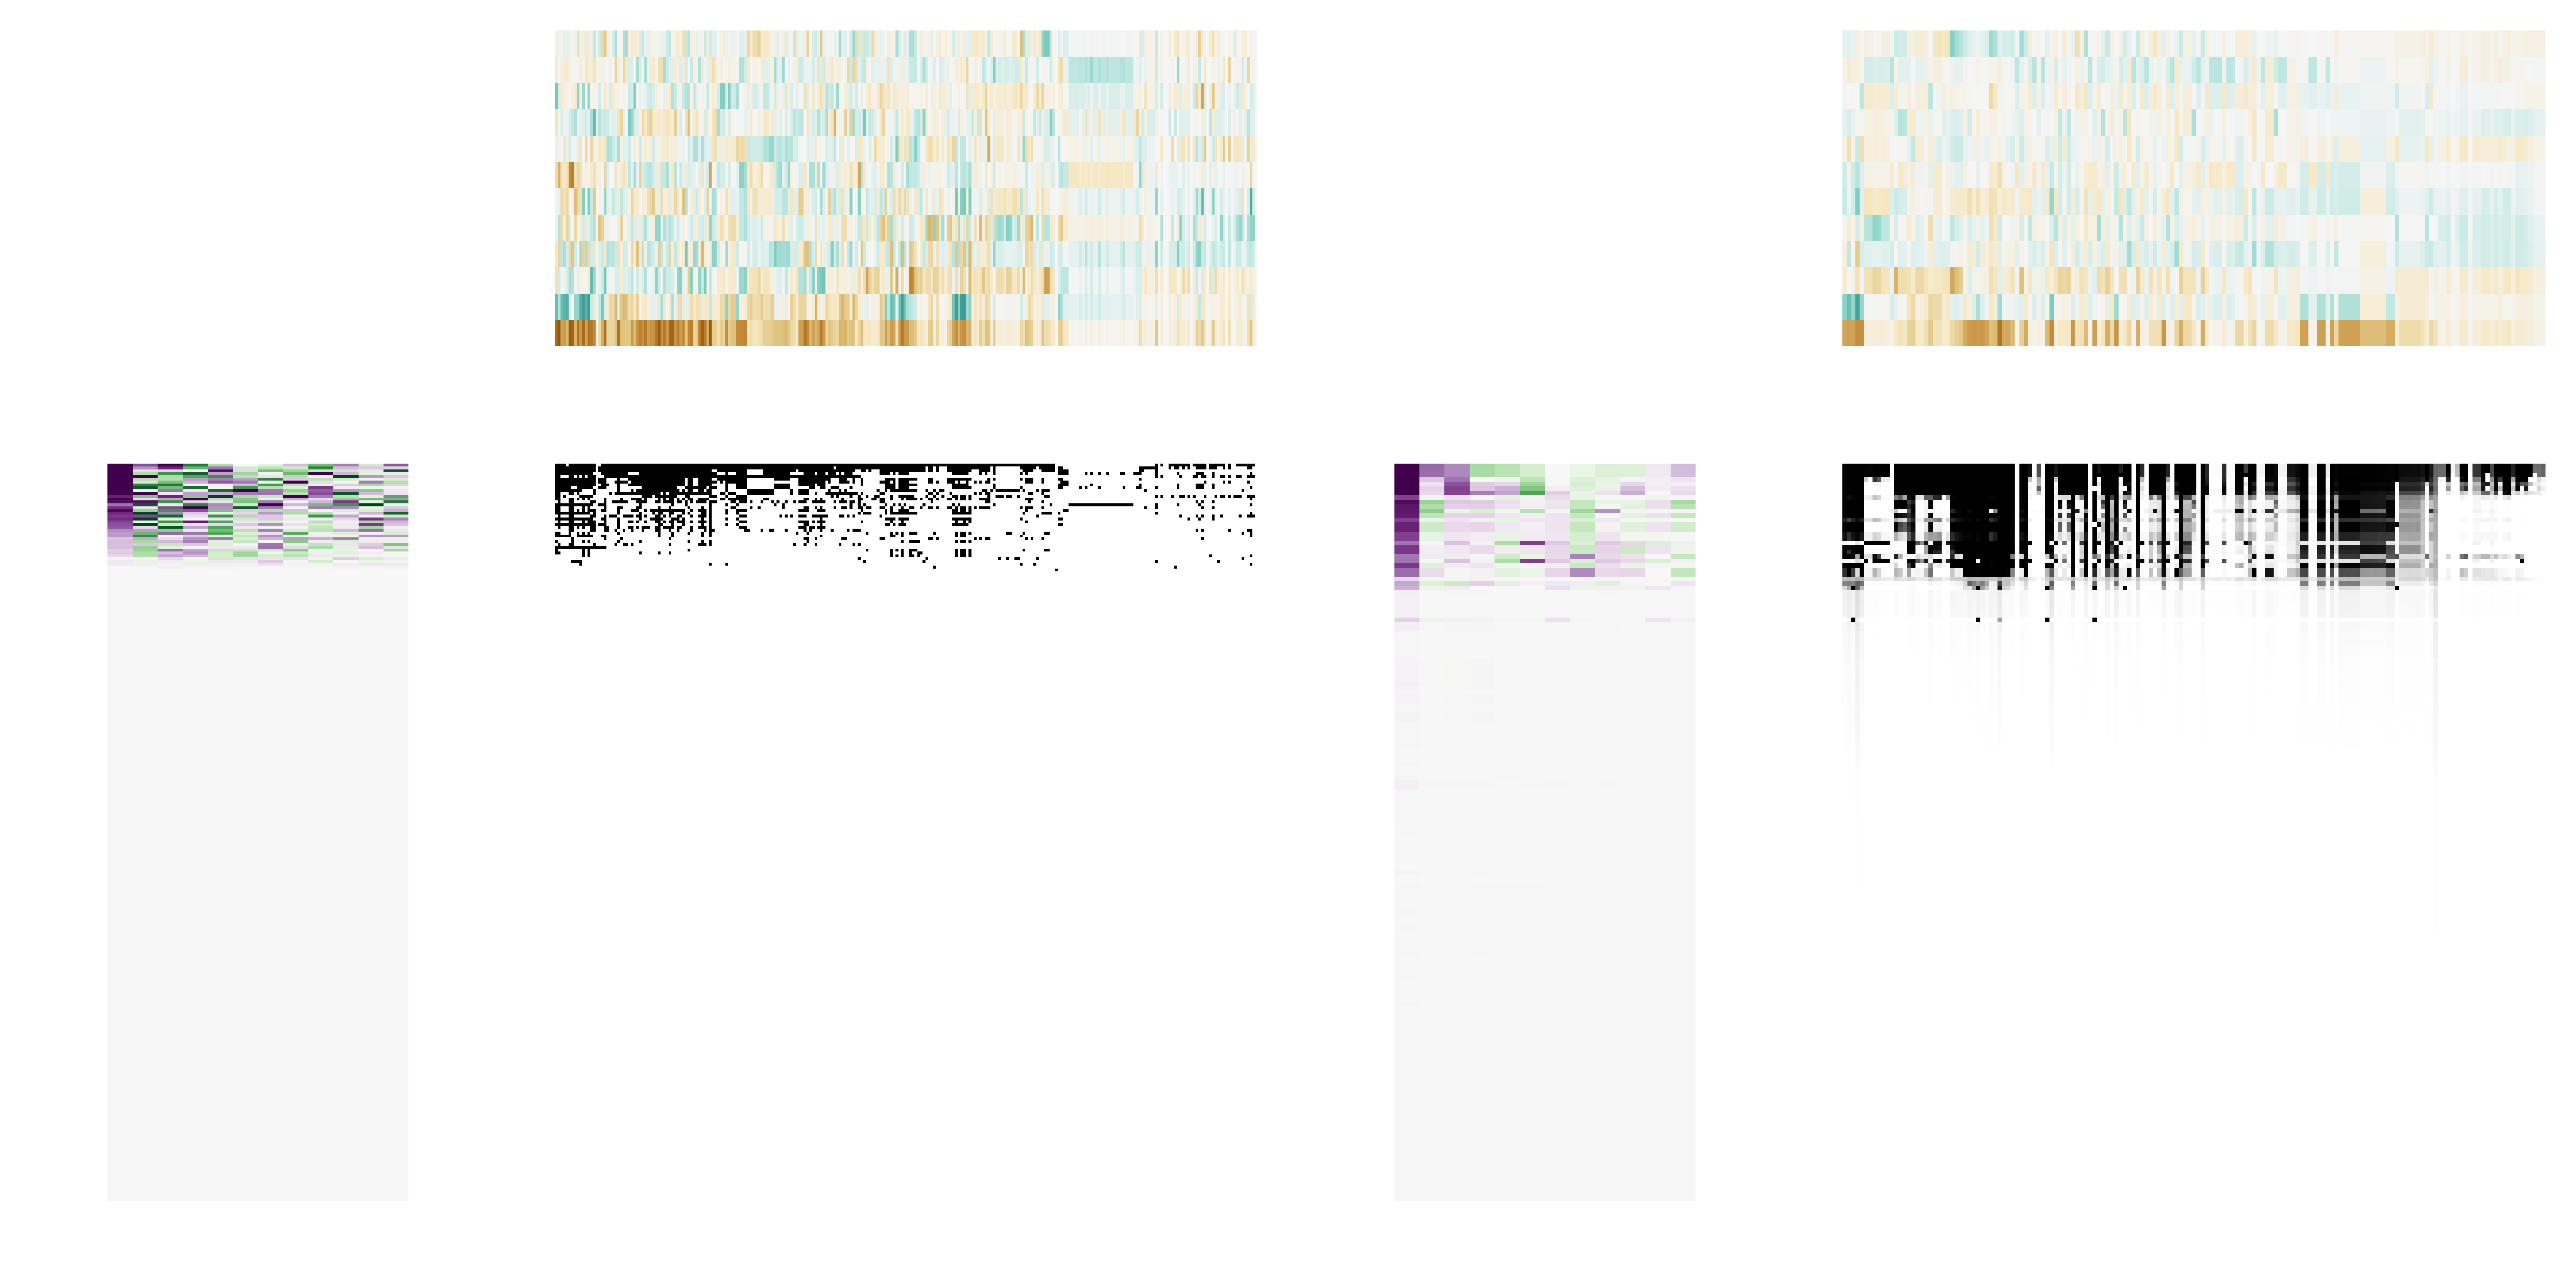
\includegraphics[width=\textwidth]{figures/figure-subspaces.png}
    \caption{Visual representation of the left (green/purple; left-side
matrix) and right (green/brown; top matrix) subspaces, alongside the
adjacency matrix of the food web they encode (grey scale). Where the
color saturation is the magnitude of the latent trait value. The
European metaweb is on the left, and the imputed Canadian metaweb
(before data inflation) on the right. This figure illustrates how much
structure the left subspace captures. As we show in @fig:degree, the
species with a value of 0 in the left subspace are species without any
prey.}
    \label{fig:subspaces}
\end{figure}

Specifically, we have adopted the following approach. For every entry in
($\hat{\mathscr{L}}$) and ($\hat{\mathscr{R}}$), we draw a value from
its distribution. This results in one instance of the possible left
($\hat{l}$) and right ($\hat{r}$) subspaces for
the Canadian metaweb. These can be multiplied, to produce one matrix of
real values. Because the entries in $\hat{l}$ and
$\hat{r}$ are in the same space where ($\mathscr{L}$) and
($\mathscr{R}$) were originally predicted, it follows that the threshold
($\rho$) estimated for the European metaweb also applies. We use this
information to produce one random Canadian metaweb,
\(N = \hat{\mathscr{L}}\hat{\mathscr{R}}' \ge \rho\). As we can see in
(\autoref{fig:subspaces}), the European and Canadian metawebs are structurally
similar (as would be expected given the biogeographic similarities) and
the two (left and right) subspaces are distinct \emph{i.e.,} capturing
predation (generality) and prey (vulnerability) latent traits.

Because the intervals around some trait values can be broad (in fact,
probably broader than what they would actually be, see \emph{e.g.,}
\cite{Garland1999Introduction}), we repeat the above process \(2\times 10^5\)
times, which results in a probabilistic metaweb \(P\), where the
probability of an interaction (here conveying our degree of trust that
it exists given the inferred trait distributions) is given by the number
of times where it appears across all random draws \(N\), divided by the
number of samples. An interaction with \(P_{i,j} = 1\) means that these
two species were predicted to interact in all \(2\times 10^5\) random
draws.

It must be noted that despite bringing in a large amount of information
from the European species pool and interactions, the Canadian metaweb
has distinct structural properties. Following an approach similar to
\cite{Vermaat2009Major}, we show in \autoref{rdpg-reconstructed-networks-have-diverse-structures} that not only can we observe
differences in the multivariate space between the European and Canadian
metawebs, we can also observe differences in the same space between
random subgraphs from these networks. These results line up with the
studies spatializing metawebs that have been discussed in the
introduction: changes in the species pool are driving local structural
changes in the networks.

\subsection{Data cleanup, discovery, validation, and
thresholding}\label{data-cleanup-discovery-validation-and-thresholding}

Once the probabilistic metaweb for Canada has been produced, we followed
a number of data inflation steps to finalize it. This step is external
to the actual transfer learning framework but rather serves as a way to
augment and validate the predicted metaweb.

\begin{figure}[h]
    \centering
    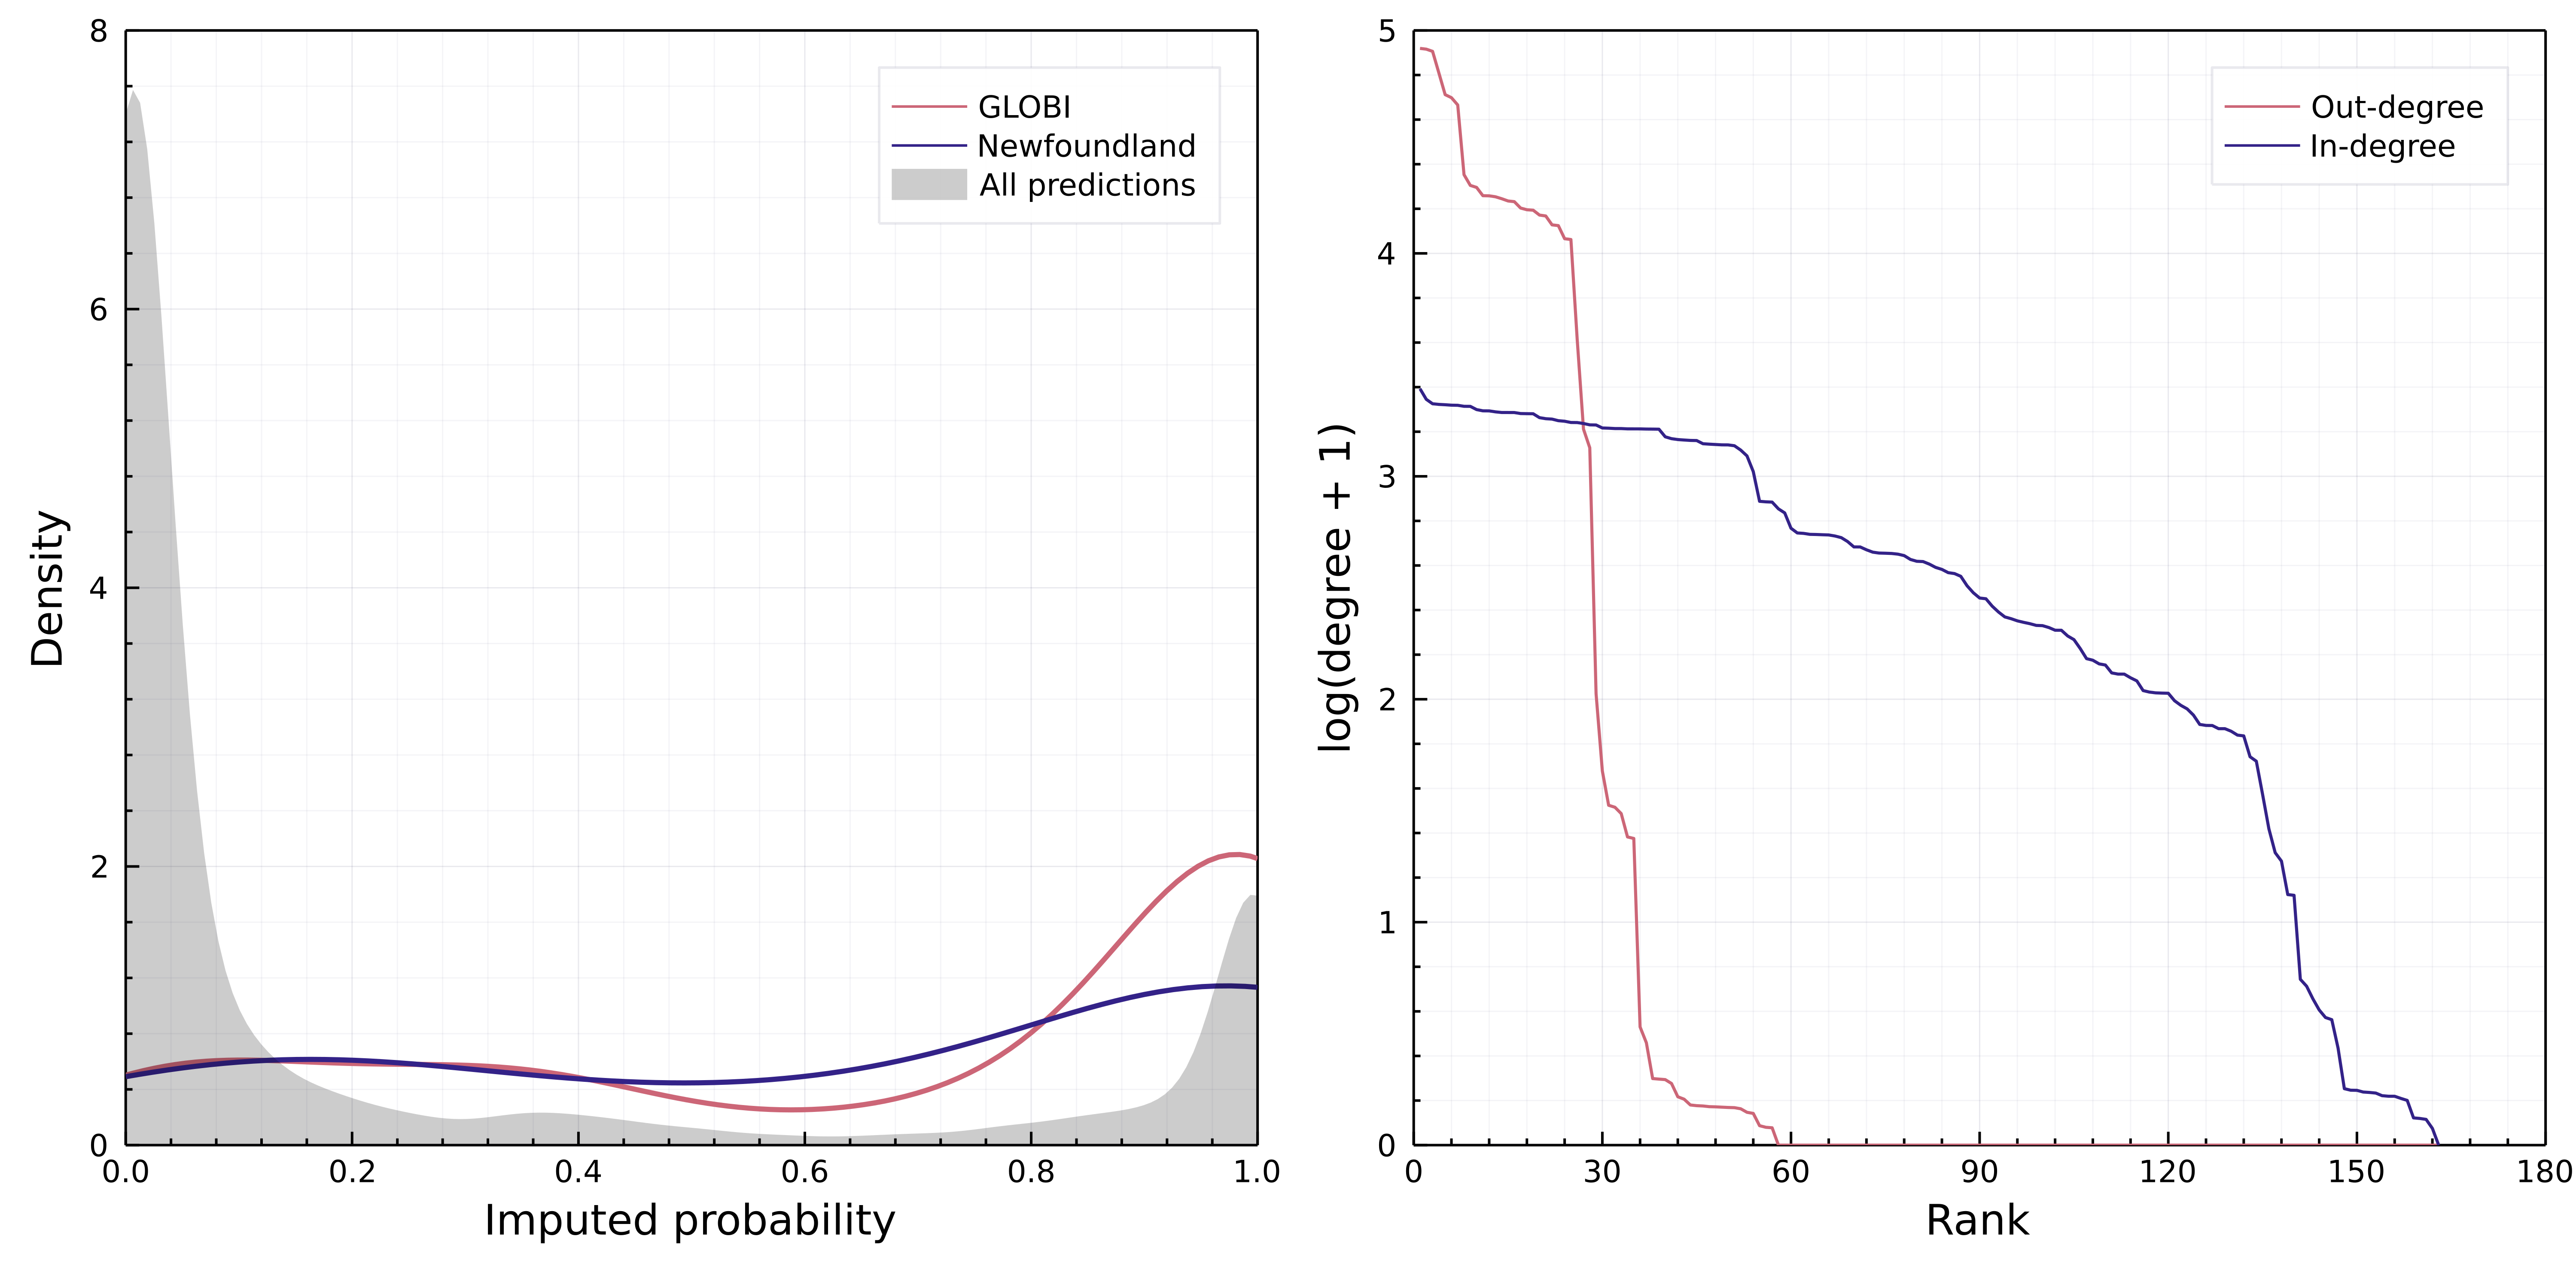
\includegraphics[width=\textwidth]{figures/figure-validation.png}
    \caption{Left: comparison of the probabilities of interactions assigned
by the model to all interactions (grey curve), the subset of
interactions found in GloBI (red), and in the \cite{Strong2014Impact}
Newfoundland dataset (blue). The model recovers more interactions with a
low probability compared to data mining, which can suggest that
collected datasets are biased towards more common or easy to identify
interactions. Right: distribution of the in-degree and out-degree of the
mammals from Canada in the reconstructed metaweb, where the rank is the
maximal number of linearly independent columns (interactions) in the
metaweb. This figure describes a flat, relatively short food web, in
which there are few predators but a large number of
preys.}
    \label{fig:inflation}
\end{figure}

First, we extracted the network corresponding to the 17 species shared
between the European and Canadian pools and replaced these interactions
with a probability of 0 (non-interaction) or 1 (interaction), according
to their value in the European metaweb. This represents a minute
modification of the inferred network (about 0.8\% of all species pairs
from the Canadian web), but ensures that we are directly re-using
knowledge from Europe.

Second, we looked for all species in the Canadian pool known to the
Global Biotic Interactions (GloBI) database \cite{Poelen2014Global}), and
extracted their known interactions. Because GloBI aggregates observed
interactions, it is not a \emph{networks} data source, and therefore the
only information we can reliably extract from it is that a species pair
\emph{was reported to interact at least once}. This last statement
should yet be taken with caution, as some sources in GloBI (\emph{e.g.,}
\cite{Thessen2014Knowledge}) are produced through text analysis, and therefore
may not document direct evidence of the interaction. Nevertheless,
should the predictive model work, we would expect that a majority of
interactions known to GloBI would also be predicted. We retrieved 366
interactions between mammals from the Canadian species pool from GloBI,
33 of which were not predicted by the model; this results in a success
rate of 91\%. After performing this check, we set the probability of all
interactions known to GloBI to 1.

Finally, we downloaded the data from \cite{Strong2014Impact}, who mined
various literature sources to identify trophic interactions in
Newfoundland. This dataset documented 25 interactions between mammals,
only two of which were not part of our (Canada-level) predictions,
resulting in a success rate of 92\%. These two interactions were added
to our predicted metaweb with a probability of 1. A comparison of
interaction densities for the inferred metaweb, and the Globi and
Newfoundland is shown in Fig.\ref{fig:inflation} and a table listing all
interactions in the predicted Canadian metaweb can be found in the
supplementary material.

\begin{figure}[h]
    \centering
    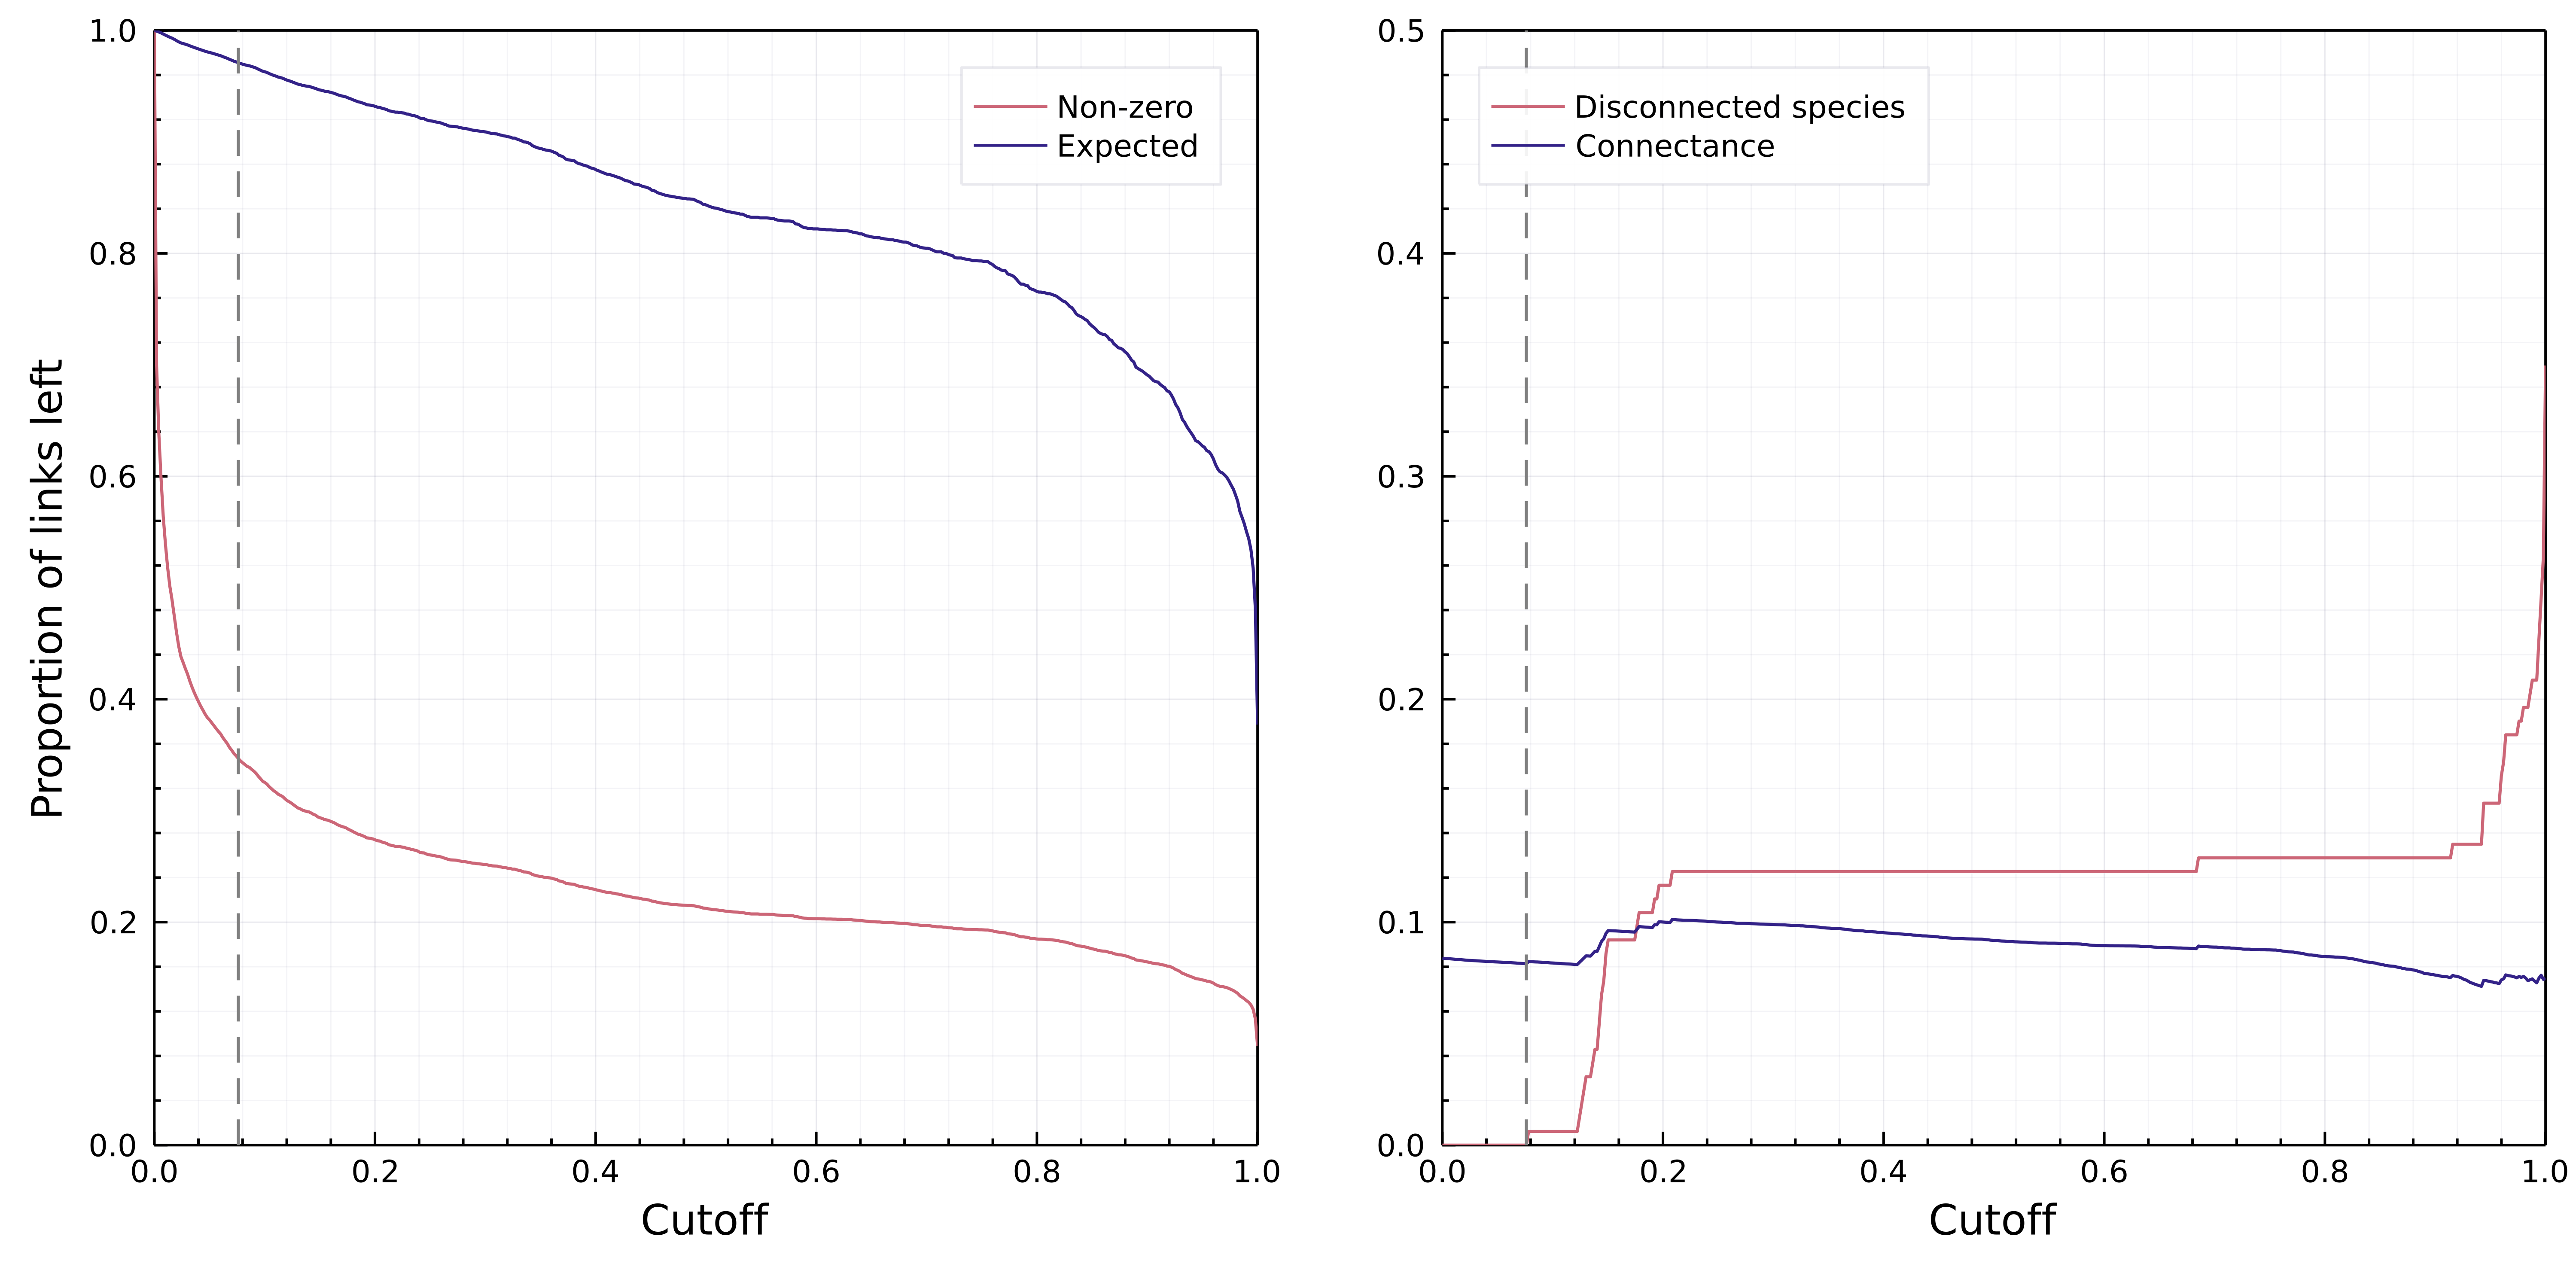
\includegraphics[width=\textwidth]{figures/figure-cutoffs.png}
    \caption{Left: effect of varying the cutoff for probabilities to be
considered non-zero on the number of unique links and on \(\hat{L}\),
the probabilistic estimate of the number of links assuming that all
interactions are independent. Right: effect of varying the cutoff on the
number of disconnected species, and on network connectance. In both
panels, the grey line indicates the cutoff
\(P(i\rightarrow j) \approx 0.08\) that resulted in the first species
losing all of its interactions.}
    \label{fig:thresholds}
\end{figure}

Because the confidence intervals on the inferred trait space are
probably over-estimates, we decided to apply a thresholding step to the
interactions after data inflation (see Fig.\ref{fig:thresholds} showing the
effect of varying the cutoff on \(P(i \rightarrow j)\)).
\cite{Cirtwill2021Building} proposed a number of strategies to threshold
probabilistic networks. Their methodology assumes the underlying data to
be tag-based sequencing, which represents interactions as co-occurrences
of predator and prey within the same tags; this is conceptually
identical to our Bernoulli-trial based reconstruction of a probabilistic
network. We performed a full analysis of the effect of various cutoffs,
and as they either resulted in removing too few interactions, or
removing enough interactions that species started to be disconnected
from the network, we set this threshold for a probability equivalent to
0 to the largest possible value that still allowed all species to have
at least one interaction with a non-zero probability. The need for this
slight deviation from the \cite{Cirtwill2021Building} methodology highlights the need for additional development on network thresholding.

\section{Results and discussion}\label{results-and-discussion}

\begin{figure}[h]
    \centering
    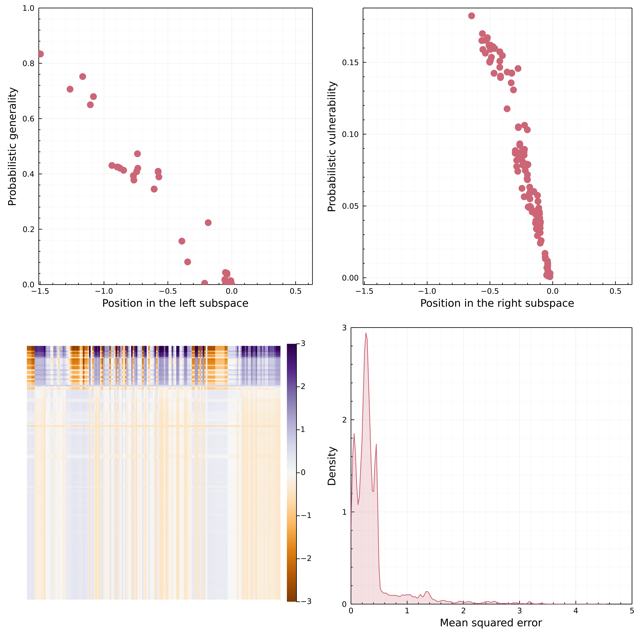
\includegraphics[width=\textwidth]{figures/figure-degree.png}
    \caption{Top: biological significance of the first dimension. Left:
there is a linear relationship between the values on the first dimension
of the left subspace and the generality, \emph{i.e.,} the relative number
of preys, \emph{sensu} \cite{Schoener1989Food}. Species with a value of 0 in
this subspace are at the bottom-most trophic level. Right: there is,
similarly, a linear relationship between the position of a species on
the first dimension of the right subspace and its vulnerability,
\emph{i.e.,} the relative number of predators. Taken together, these two
figures show that the first-order representation of this network would
capture its degree distribution. Bottom: topological consequences of the
first dimension. Left: differences in the \(z\)-scores of the actual
configuration model for the reconstructed network and the prediction
based only on the first dimension (with a deeper saturation indicating a
bigger difference in scores). Right: distribution of the differences in
the left panel.}
    \label{fig:degree}
\end{figure}

Using a transfer learning framework we were able to construct a
probabilistic metaweb and (as per \cite{Dunne2006Network}) is a list of
potential interactions, meaning that they will not necessarily be
realized wherever the two species co-occur. The t-SVD embedding is able
to learn relevant ecological features for the network. Fig.\ref{fig:degree} shows
that the first rank correlates linearly with generality and
vulnerability (\cite{Schoener1989Food}), \emph{i.e.,} the number of preys
and predators for each species. Importantly, this implies that a rank 1
approximation represents the configuration model for the metaweb,
\emph{i.e.,} a set of random networks generated from a given degree
sequence (\cite{Park2004Statistical}). Accounting for the probabilistic nature
of the degrees, the rank 1 approximation also represents the \emph{soft}
configuration model (\cite{vanderHoorn2018Sparse}). Both models are
maximum entropy graph models (\cite{Garlaschelli2018Covariance}), with sharp
(all network realizations satisfy the specified degree sequence) and
soft (network realizations satisfy the degree sequence on average) local
constraints, respectively. The (soft) configuration model is an unbiased
random graph model widely used by ecologists in the context of null
hypothesis significance testing of network structure (\emph{e.g.,}
\cite{Bascompte2003Nested}) and can provide informative priors for Bayesian
inference of network structure (\emph{e.g.,} \cite{Young2021Bayesian}). It is
noteworthy that for this metaweb, the relevant information was extracted
at the first rank. Because the first rank corresponds to the leading
singular value of the system, the results of Fig.\ref{fig:degree} have a
straightforward interpretation: degree-based processes are the most
important in structuring the mammalian food web.

One important aspect in which Europe and Canada differ (despite their
comparable bioclimatic conditions) is the degree of the legacy of human
impacts, which have been much longer in Europe. \cite{Nenzen2014Impact} showed
that even at small scales (the Iberian peninsula), mammal food webs
retain the signal of both past climate change and human activity, even
when this human activity was orders of magnitude less important than it
is now. Similarly, \cite{Yeakel2014Collapse} showed that changes in human
occupation over several centuries can lead to food web collapse.
Megafauna in particular seems to be very sensitive to human arrival
(\cite{Pires2015Pleistocene}). In short, there is well-substantiated support
for the idea that human footprint affects more than the risk of species
extinction (\cite{Marco2018Changes}), and can lead to changes in
interaction structure.

\cite{Cirtwill2019QuaFra} showed that network inference techniques based on
Bayesian approaches would perform far better in the presence of an
interaction-level informative prior; the desirable properties of such a
prior would be that it is expressed as a probability, preferably
representing a Bernoulli event, the value of which would be
representative of relevant biological processes (probability of
predation in this case). We argue that the probability returned at the
very last step of our framework may serve as this informative prior;
indeed, the output of our analysis can be used in subsequent steps, also
possibly involving expert elicitation to validate some of the most
strongly recommended interactions. One important \emph{caveat} to keep
in mind when working with interaction inference is that interactions can
never really be true negatives (in the current state of our
methodological framework and data collection limitations); this renders
the task of validating a model through the usual application of binary
classification statistics very difficult (although see
\cite{Strydom2021Roadmap} for a discussion of alternative suggestions). The
other way through which our framework can be improved is by substituting
the predictors that are used for transfer. For example, in the presence
of information on species traits that are known to be predictive of
species interactions, one might want to rely on functional rather than
phylogenetic distances -- in food webs, body size (and allometrically
related variables) has been established as such a variable
(\cite{Brose2006Consumer}); the identification of relevant functional traits
is facilitated by recent methodological developments
(\cite{Rosado2013Going}).

Finally, it should be noted that the framework we have presented is
amenable to changes lending to applicability to a broad range of
potential scenarios. For example in this case study we have embedded the
original metaweb using t-SVD, because it lends itself to an RDPG
reconstruction, which is known to capture the consequences of
evolutionary processes (\cite{DallaRiva2016Exploring}); this being said,
there are other ways to embed graphs (\cite{Arsov2019Network, Cai2017Comprehensive, Cao2019Network}), which can be used as alternatives.
Regarding the transfer step it is possible to use distinct trees if
working with distinct clades (such as pollination networks) or an
alternative measure of similarity (transfer medium) such as information
on foraging (\cite{Beckerman2006Foraging}), cell-level mechanisms
(\cite{Boeckaerts2021Predicting}), or a combination of traits and phylogenetic
structure (\cite{Stock2021Pairwise}). Most importantly, although we focus on
a trophic system, it is an established fact that different (non-trophic)
interactions do themselves interact with and influence the outcome of
trophic interactions (see \emph{e.g.,} \cite{Kawatsu2021Are, Kefi2012More}). Future development of metaweb inference techniques
should cover the prediction of multiple interaction types.

\textbf{Acknowledgements:} We acknowledge that this study was conducted
on land within the traditional unceded territory of the Saint Lawrence
Iroquoian, Anishinabewaki, Mohawk, Huron-Wendat, and Omàmiwininiwak
nations. TP, TS, DC, and LP received funding from the Canadian Institute
for Ecology \& Evolution. FB is funded by the Institute for Data
Valorization (IVADO). TS, SB, and TP are funded by a donation from the
Courtois Foundation. CB was awarded a Mitacs Elevate Fellowship no.
IT12391, in partnership with fRI Research, and also acknowledges funding
from Alberta Innovates and the Forest Resources Improvement Association
of Alberta. M-JF acknowledges funding from NSERC Discovery Grant and
NSERC CRC. RR is funded by New Zealand's Biological Heritage Ngā Koiora
Tuku Iho National Science Challenge, administered by New Zealand
Ministry of Business, Innovation, and Employment. BM is funded by the
NSERC Alexander Graham Bell Canada Graduate Scholarship and the FRQNT
master's scholarship. LP acknowledges funding from NSERC Discovery Grant
(NSERC RGPIN-2019-05771). TP acknowledges financial support from NSERC
through the Discovery Grants and Discovery Accelerator Supplement
programs. MJF is supported by an NSERC PDF and an RBC Post-Doctoral
Fellowship

\printbibliography{}
\end{refsection}

\endinput
%%
%% End of file `article1.tex'.

%%
%% This is file `article1.tex', % generated with the docstrip utility.
%%
%% The original source files were:
%%
%% dms.dtx  (with options: `article') % Example TeX file for the documentation %
%of the jurabib package % Copyright (C) 1999, 2000, 2001 Jens Berger % See
%dms.ins  for the copyright details.
%% 
%%% ====================================================================
%%%  @LaTeX-file{ %%     filename        = "dms.dtx", %%     author    =
%"Nicolas Beauchemin, Damien Rioux-Lavoie, Victor Fardel, Jonathan Godin", %%
%copyright = "Copyright (C) 2000 , DMS %%                  all rights reserved.
%Copying of this file is %%                  authorized only if either: %%
%(1) you make absolutely no changes to your copy, %%                  including
%name; OR %%                  (2) if you do make changes, you first rename it %%
%to some other name.", %%     address   = "Département de Mathématiques et de
%Statistique", %%     telephone = "514-343-6705", %%     FAX       =
%"514-343-5700", %%     email     = "aide@dms.umontreal.ca (Internet)", %%
%keywords  = "latex, amslatex, ams-latex, theorem", %%     abstract  = " Ce
%fichier est un package conçu pour être %%                  utilisé avec la
%version de LaTeX2e 1995/06/01. Il %%                  est prévue pour la classe
%``amsbook''. Il en %%                  modifie le format des pages, l'entête
%des %%                  sections, etc, afin d'être  conforme au modèle de %%
%mémoire de maîtrise de l'Université de %%                  Montréal. Finalement
%ce fichier est grandement %%                  inspiré du fichier
%amsclass.dtx.", %%     docstring = "The checksum field contains: CRC-16
%checksum, %%                  word count, line count, and character count, as
%%%                  produced by Robert Solovay's checksum utility."}
%%%  ====================================================================


%% To change chapter header dynamically from french to english, use
%%\entetedynamique
\setcounter{corA}{0} % Pour recommancer à compter les def,
                     % theo, etc. à partir de 1
 % Pour écrire un article en français
%% \francais
 % Pour écrire un article en anglais
\anglais
%% NOTE: La plupart des macros ont un nom en anglais. % P.ex. \adresse et
%\address fonctionnent et sont équivalents. % \revue=\journal % \auteur=\author
%% \titre=\title

\doublespacing

%% Les contributions apparaîtront habituellement après % \maketitle (voir un peu
%plus bas). Selon les goûts, il est % possible de mettre les contributions %
%avant la page titre de l'article, simplement en les écrivant % directement ici.
%Par exemple :
 % \cleardoublepage \pdfbookmark[chapter]{Contributions}{contrib1} % Remplacer
 % par contrib2 pour l'article 2 etc. {\bfseries\Large\noindent Contributions de
 % <mon nom> et rôle joué par les coauteurs} J'ai contribué en...
 %
 % Le rôle des coauteurs a été de...

%% Nom de la revue de publication
\revue{Frontiers in Ecology and Evolution and can be found at https://doi.org/10.3389/fevo.2021.623141}
\article{SVD Entropy reveals the high complexity of ecological networks}\label{SVD}
%% On peut se référer aux numéros de chapitre ou d'article comme suit. % Si on
%fait % \label{chap:article1}, % alors \ref{chap:article1} donnera le numéro du
%chapitre. On peut ensuite faire % \labelart{art:article1} % et alors
%\ref{art:article1} donnera le numéro d'article. % Par exemple, si cette article
%est le premier article et le deuxième chapitre, % alors si on écrit % Voir le
%chapitre~\ref{chap:article1} (l'article~\ref{art:article1}). % deviendra % Voir
%le chapitre 2 (l'article 1). % Si on veut écrire « premier article » au lieu «
%article 1 », on peut % simplement faire % \ordinal{\ref{art:article1}}~article
%% devient première article % ou % \Ordinal{\ref{art:article1}}~article  %
%devient Première article (avec la majuscule) % Si on est en mode \anglais,
%\ordinal écrire first, second,...

%%%%%%%%%%%%%%%%%%%%%%%%%%%%%%%%%%%%%%%%%%%%%%%%%%%%%%%%%%%%%%%
%%%%%%%%%%%%%%%%%     Contribution     %%%%%%%%%%%%%%%%%%%%%%%% %%%%%%%%%%%%%%%%
%(lire attentivement) %%%%%%%%%%%%%%%%%%%%%%%%
%%%%%%%%%%%%%%%%%%%%%%%%%%%%%%%%%%%%%%%%%%%%%%%%%%%%%%%%%%%%%%%
 % Contribution(s) peronnelle(s) à l'article et rôle joué par tous les
 % coauteur·e·s
 %
 % Nécessaire seulement lorsque vous n'êtes pas seul·e auteur·e. Les
 % contributions peuvent apparaître ailleur dans la thèse. Si \contributions est
 % laissé vide (p.ex. si vous effacez celui ci-bas), aucune contributions ne
 % seront générées sur la page titre de l'article. Vous pouvez alors mettre un
 % \newpage si vous souhaitez que les résumé et abstract soient sur la page
 % suivante.
 %
 % REMARQUE : À peu près toutes les constructions \LaTeX\ sont permises dans les
 % contributions.
 %
 % La commande admet une option [<entête>]
\contributions%[Mes contributions et le rôle des coauteurs]
{ 

TP and TS designed the study and edited the manuscript for submission. TS performed the analysis and wrote the manuscript. All authors contributed to the article and approved the submitted version.\\[1cm]
}

%%% INFORMATIONS POUR LA PAGE TITRE
 % Premier auteur·e et adresse

\auteur{Tanya Strydom}
\adresse{Département de Sciences Biologiques, Université de Montréal, Montreal, QC, Canada\\ Québec Centre for Biodiversity Sciences, Montreal, QC, Canada}
\auteur{Giulio V. Dalla Riva}
\adresse{School of Mathematics and Statistics, University of Canterbury, Christchurch, New Zealand}
\auteur{Timothée Poisot}
\adresse{Département de Sciences Biologiques, Université de Montréal, Montreal, QC, Canada\\ Québec Centre for Biodiversity Sciences, Montreal, QC, Canada}
%

\maketitle

\begin{resume}{décomposition en valeurs singulières, complexité physique, réseau bipartite, entropie, pollinisation, analyse de réseaux écologiques} Quantifier la complexité des réseaux écologiques reste difficile à évaluer. Principalement, la complexité a été définie sur la base de la complexité structurelle (ou comportementale) du système. Ces définitions ignorent la notion de « complexité physique », qui peut mesurer la quantité d’informations contenues dans un réseau écologique et la difficulté de les compresser. Nous présentons respectivement le déficit de rang relatif et l’entropie SVD comme mesures de la complexité "externe" et "interne". En utilisant des réseaux écologiques bipartites, nous constatons qu’ils présentent tous une complexité physique très élevée, presque maximale. Les réseaux de pollinisation, en particulier, sont plus complexes que d’autres types d’interactions. De plus, nous constatons que l'entropie SVD est liée à d'autres mesures structurelles de complexité (imbrication, connectivité et rayon spectral), mais ne renseigne pas sur la résilience d'un réseau lors de l'utilisation de cascades d'extinction simulées, ce qui a déjà été rapporté pour des mesures structurelles de complexité. Nous soutenons que l’entropie SVD fournit une mesure fondamentalement plus "correcte" de la complexité des réseaux et devrait être ajoutée à la boîte à outils des descripteurs des réseaux écologiques à l’avenir.
\end{resume}

\begin{abstract}{singular value decomposition, physical complexity, bipartite network, entropy, pollination, ecological network analysis} Quantifying the complexity of ecological networks has remained elusive. Primarily, complexity has been defined on the basis of the structural (or behavioural) complexity of the system. These definitions ignore the notion of “physical complexity,” which can measure the amount of information contained in an ecological network, and how difficult it would be to compress. We present relative rank deficiency and SVD entropy as measures of “external” and “internal” complexity, respectively. Using bipartite ecological networks, we find that they all show a very high, almost maximal, physical complexity. Pollination networks, in particular, are more complex when compared to other types of interactions. In addition, we find that SVD entropy relates to other structural measures of complexity (nestedness, connectance, and spectral radius), but does not inform about the resilience of a network when using simulated extinction cascades, which has previously been reported for structural measures of complexity. We argue that SVD entropy provides a fundamentally more “correct” measure of network complexity and should be added to the toolkit of descriptors of ecological networks moving forward.
\end{abstract}

\begin{refsection}

\section{Introduction}

Ecologists have turned to network theory because it offers a powerful
mathematical formalism to embrace the complexity of ecological communities
(\cite{Bascompte2007PlaMut}). Indeed, analysing ecological systems as networks
highlighted how their structure ties into ecological properties and processes
(\cite{Proulx2005NetThi, Poulin2010NetAna}), and there has been a subsequent
explosion of measures that purport to capture elements of network structure, to be related to the ecology of the system they describe (\cite{Delmas2018Analysing}). Since the early days of network ecology, ecological networks have been called
``complex''. This sustained interest for the notion of complexity stems, in
part, from the strong ties it has to stability (\cite{Landi2018Complexity}). As such,
many authors have looked for clues, in the network structure, as to why the
networks do not collapse (\cite{Borrelli2015SelIns, Staniczenko2013GhoNes,
Gravel2016StaCom, Brose2006AllSca}). Yet decades of theoretical refinements on
the relationship between complexity and stability had a hard time when
rigorously tested on empirical datasets (\cite{Jacquet2016NoCom}); although
ecological networks may be complex, our current measures of complexity do not
translate into predictions about stability.

Surprisingly, \emph{complexity} itself has proven an elusive concept to define
in a rigorous way. It has over time been defined as connectance
(\cite{Rozdilsky2001ComCan}), as measures of the diversity of species or their
interactions (\cite{Landi2018Complexity}), or as a combination of species richness and trophic diversity (\cite{Duffy2007FunRol}). In short, network ecology as a field readily assumes that because we have more information about a system, or because this system has more components, or simply because this system can be expressed as a network, it follows that the system is complex. But such a diversity of definitions, for a concept that is so central to our quest to understand network stability, decreases the clarity of what complexity means, and what all of these alternative definitions do actually capture. This is a common thread in some measures of ecological network structure, as has been discussed at length for
the various definitions of nestedness (\cite{Ulrich2009ConSG}).

None of the previous definitions of complexity are formally wrong, in that they do capture an aspect of complexity that ultimately ties to the behaviour of the system, \emph{i.e.,} its low predictability over time. Yet
(\cite{Adami2002WhaCom}) provides a compelling argument for why the
complexity of the behaviour does not necessarily reflects the complexity of the
system; in fact, one would be very hard pressed to think of a more simple system
than the logistic map used by \cite{May1976SimMat} to illustrate how easily
complexity of behaviour emerges. Rather than yielding to the easy assumption
that a system will be complex because it has many parts, or because it exhibits
a complex behaviour, \cite{Adami2002WhaCom} suggests that we focus on
measuring ``physical complexity'', \emph{i.e.,} the amount of information
required to encode the system, and how much signal this information contains.
Complex systems, in this perspective, are those who cannot easily be compressed
- and this is a notion we can explore for the structure of ecological networks.

Ecological networks are primarily represented by their adjacency matrices,
\emph{i.e.,} a matrix in which every entry represents a pair of species, which
can take a value of 1 when the two species interact, and a value of 0 when they
do not. These matrices (as any matrices) can easily be factorised using Singular
Value Decomposition (\cite{Forsythe1967ComSol, Golub1971SinVal}), which offers two
interesting candidate measures of complexity for ecological networks (both of
which we describe at length in the methods). The first measure is the rank of
the matrix, which works as an estimate of ``external complexity'', in that it
describes the dimension of the vector space of this matrix, and therefore the
number of linearly independent rows (or columns) of it. From an ecological
standpoint, this quantifies the number of unique ``strategies'' represented in
the network: a network with two modules that are distinct complete graphs has a
rank of 2. The second measure is an application of the entropy measure of
\cite{Shannon1948MatThe} to the non-zero singular values of the matrix
obtained through SVD. This so-called SVD entropy measures the extent to which
each rank encodes an equal amount of information, as the singular values capture
the importance of each rank to reconstruct the original matrix; this approach
therefore serves as a measure of ``internal complexity''.

In this manuscript, we present and evaluate the use of both the rank and SVD
entropy of ecological networks as alternative and more robust measures of
complexity when compared to traditional approaches to defining complexity. This
is done by using a collection of 220 bipartite networks from various types of
interaction, sizes, connectances, and environments. We show that while the rank
of the adjacency matrix holds little information, SVD entropy functions as an
appropriate quantification of the complexity of ecological systems. Notably, SVD
entropy is an intuitive, robust, non-structural approach to defining the
(surprisingly high) complexity of ecological networks, by relating them to their
`physical' as opposed to `behavioural' complexity. In this process we showcase a
breakdown in the assumption that all measures of complexity of networks are
indicative of their robustness to extinctions. Finally, we show that, despite
their high complexity, observed networks are less complex when compared to
pseudo-random networks, especially for larger networks. We propose that taking a
physical approach to quantifying the complexity of ecological networks is a step
in the right direction to unifying how we define complexity in the context of
ecological networks, as it restores other measures (like connectance and
nestedness) to their original role and signification.

\section{Data and methods}\label{data-and-methods}

We used all bipartite networks contained in the \texttt{web-of-life.es}
database. This database extracted species interaction networks from
supplementary materials across all inhabited continents and covers a large array
of sampling years, environments, organisms, and sampling methodologies. As such,
this dataset is particularly suited to describe general trends across \emph{all}
ecological networks. We specifically worked on the version of this dataset
distributed with the \texttt{EcologicalNetworks.jl} package
(\cite{Poisot2019EcoJl}) for the \emph{Julia} (\cite{Bezanson2017Julia})
programming language, in which all analyses were conducted. Using bipartite
networks means that interacting species are split into two sets (or interacting
groups) and along different dimensions in the interaction matrix. Thus, columns
in the matrix represent one group (or type) of species and rows represent the
other group of species involved in the interaction. Because SVD gives similar
results on the matrix and its transpose, it captures the complexity of both
sides of the system at once. A summary of the dataset is given in
\autoref{table:summary}.

\begin{table}[h!]
\centering
\begin{tabular}{||c c c c c||} 
 \hline
 Interaction type & Sample size & Latitude range & Richness (top) & Richness
 (bottom) \\ [0.5ex] \hline\hline
 Host-Parasite & 51 & 38.77 \(\rightarrow\) 72.65 & 20.47 & 12.23 \\ 
 Plant-Ant & 4 & -16.11 \(\rightarrow\) -2.40 & 18.75 & 21.75 \\
 Plant-Herbivore & 4 & 30.20 \(\rightarrow\) 64.91 & 49.5 & 29.25 \\
 Pollination & 134 & -43.09 \(\rightarrow\) 81.81 & 40.22 & 18.02 \\
 Seed Dispersal & 33 & -28.95 \(\rightarrow\) 53.05 & 18.75 & 25.12 \\ [1ex] 
 \hline
\end{tabular}
\caption{Overview of the \texttt{web-of-life.es} dataset. We used all networks
with up to 500 species. Although there are spatial biases in the sampling of
interaction types (and some interaction types being under-represented), this
dataset covers a range of latitudes from -43 degrees south to 81 degrees north.
The average richness of the top and bottom level of the bipartite networks are
also given in the last columns.}
\label{table:summary}
\end{table}

\subsection{Estimating complexity with rank
deficiency}\label{estimating-complexity-with-rank-deficiency}

The rank of \(\mathbf{A}\) (noted as \(r = \text{rk}(\mathbf{A})\)) is the
dimension of the vector space spanned by the matrix and corresponds to the
number of linearly independent rows or columns; therefore, the maximum rank of a
matrix (\(M = \text{rk}_{\text{max}}(\mathbf{A})\)) will always be equal to the
length of the shortest dimension of \(\mathbf{A}\), which ecologically speaking
is the richness of the least species-rich compartment of the bipartite network
(or the richness in the case of unipartite networks). A matrix is
``full-ranked'' when \(r=M\), \emph{i.e.,} all of its rows/columns are unique.
Matrices that are not full-ranked are called rank deficient, and we can measure
rank deficiency using \(d = M-r\). So as to control for the difference in
species richness of the different networks, we report the relative rank
deficiency, \emph{i.e.,} expressed as a ratio between rank deficiency and the
maximal rank:

\[D = 1-\frac{r}{M}\]\

This measure returns values between 0 (the matrix is full ranked) and \(1-M^{-1}
\approx 1\) (the matrix has rank 1). This serves as a coarse estimate of
complexity, as the more unique columns/rows are in the matrix, the larger this
value will be. Yet it may also lack sensitivity, because it imposes a stringent
test on uniqueness, which calls for more quantitative approaches to complexity.

\subsection{Estimating complexity with SVD
entropy}\label{estimating-complexity-with-svd-entropy}

Singular Value Decomposition (SVD) is the factorisation of a matrix
\(\mathbf{A}\) (where \(\mathbf{A}_{m,n} \in\mathbb{B}\) in our case, but SVD
works for matrices of real numbers as well) into the form
\(\mathbf{U}\cdot\mathbf{\Sigma}\cdot \mathbf{V}^T\). Where \(\mathbf{U}\) is an
\(m \times m\) orthogonal matrix and \(\mathbf{V}\) an \(n \times n\) orthogonal
matrix. The columns in these matrices are, respectively, the left- and
right-singular vectors of \(\mathbf{A}\), were \(\mathbf{U} =
\mathbf{A}\mathbf{A}^T\) and \(\mathbf{V} = \mathbf{A}^T\mathbf{A}\).
\(\mathbf{\Sigma}\) is a matrix that only contains non-negative \(\sigma\)
values along its diagonal and all other entries are zero. Where \(\sigma_{i} =
\Sigma{ii}\), which contains the singular values of \(\mathbf{A}\). When the
values of \(\mathbf{\sigma}\) are arranged in descending order, the singular
values (\(\mathbf{\Sigma}\)) are unique, though the singular vectors
(\(\mathbf{U}\) and \(\mathbf{V}\)) may not be.

After the Eckart-Young-Mirsky theorem (\cite{Eckart1936AppOne, Golub1987GenEck}),
the number of non-zero entries (after rounding of small values if required due
to numerical precision issues in computing the factorisation) in
\(\mathbf{\sigma}\) is the rank of matrix \(\mathbf{A}\). For the sake of
simplicity in notation, we will use \(k = \text{rk}(\mathbf{A})\)) for the rank
of the matrix. Because only the first \(k\) elements of \(\mathbf{\sigma}\) are
non-zero, and that the result of the SVD is a simple matrix multiplication, one
can define a truncated SVD containing only the first \(k\) singular values.

Intuitively, the singular value \(i\) (\(\sigma_i\)) measures how much of the
dataset is (proportionally) explained by each vector - therefore, one can
measure the entropy of \(\mathbf{\sigma}\) following \cite{Shannon1948MatThe}. High
values of SVD entropy reflects that all vectors are equally important,
\emph{i.e.,} that the structure of the ecological network cannot efficiently be
compressed, and therefore indicates high complexity (\cite{Gu2016HowLon}). Because
networks have different dimensions, we use Pielou's evenness
(\cite{Pielou1975EcoDiv}) to ensure that values are lower than unity, and quantify
SVD entropy, using \(s_i = \sigma_i/\text{sum}(\sigma)\) as:

\[J = -\frac{1}{\ln(k)}\sum_{i=1}^k s_i\cdot\ln(s_i)\]\

\section{Results and discussion}\label{results-and-discussion-svd}

\subsection{Most ecological networks are close to
full-rank}\label{most-ecological-networks-are-close-to-full-rank}

The majority (63\% of our dataset) of bipartite ecological networks have a
relative rank deficiency of 0 (\autoref{fig:size}), which indicates that all
species have different and unique interaction lists. Interestingly, the networks
that had a comparatively larger relative rank deficiency tended to be smaller
ones. Yet because most of the networks return the same value, matrix rank does
not appear to be a useful or discriminant measure of network complexity. Another
striking result (from \autoref{fig:size}) is that the SVD entropy of ecological
networks is really large -- although the value can range from 0 to 1, all
ecological networks had SVD entropy larger than 0.8, which is indicative of a
strong complexity.

\begin{figure}[h]
    \centering
    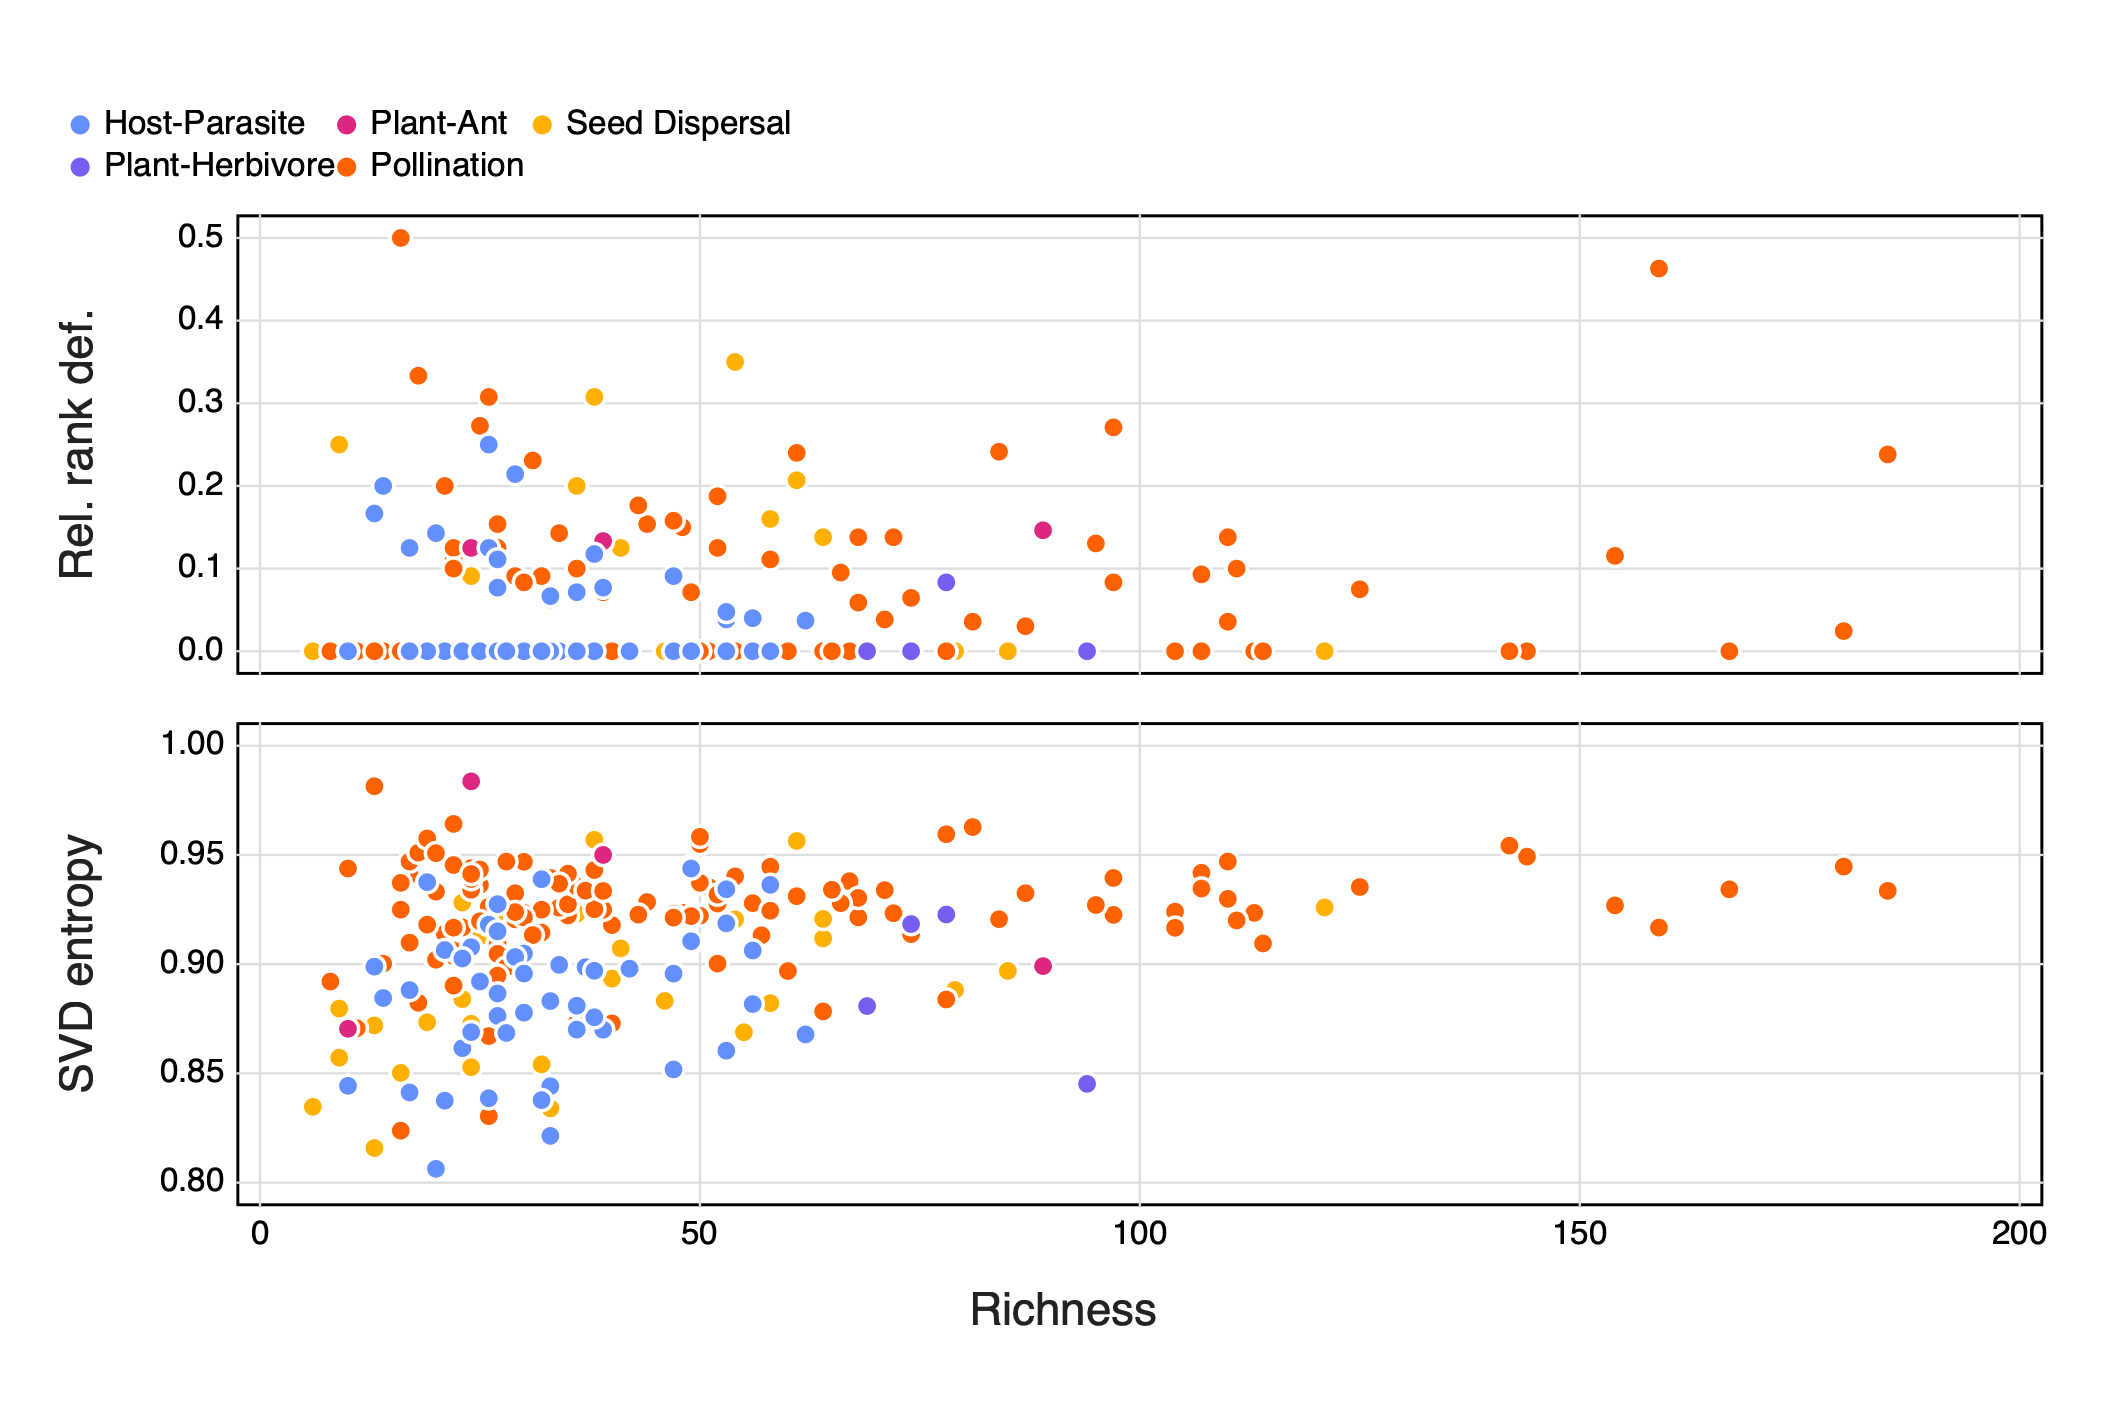
\includegraphics[width=\textwidth]{figures/size_v_rankentropy.png}
    \caption{The relationship between network richness and relative rank
deficiency, and SVD entropy. The different types of interactions are indicated
by the colours.}
    \label{fig:size}
\end{figure}

As expected following the observation that ecological networks are
overwhelmingly full ranked, we do not see a relationship between SVD entropy and
relative rank deficiency, neither do we observe differences between interaction
types (\ref{fig:entropy_v_rank}). Based on these results, we feel confident that
SVD entropy provides a more informative measure of the complexity of ecological
networks, and will use it moving forward.

\begin{figure}[h]
    \centering
    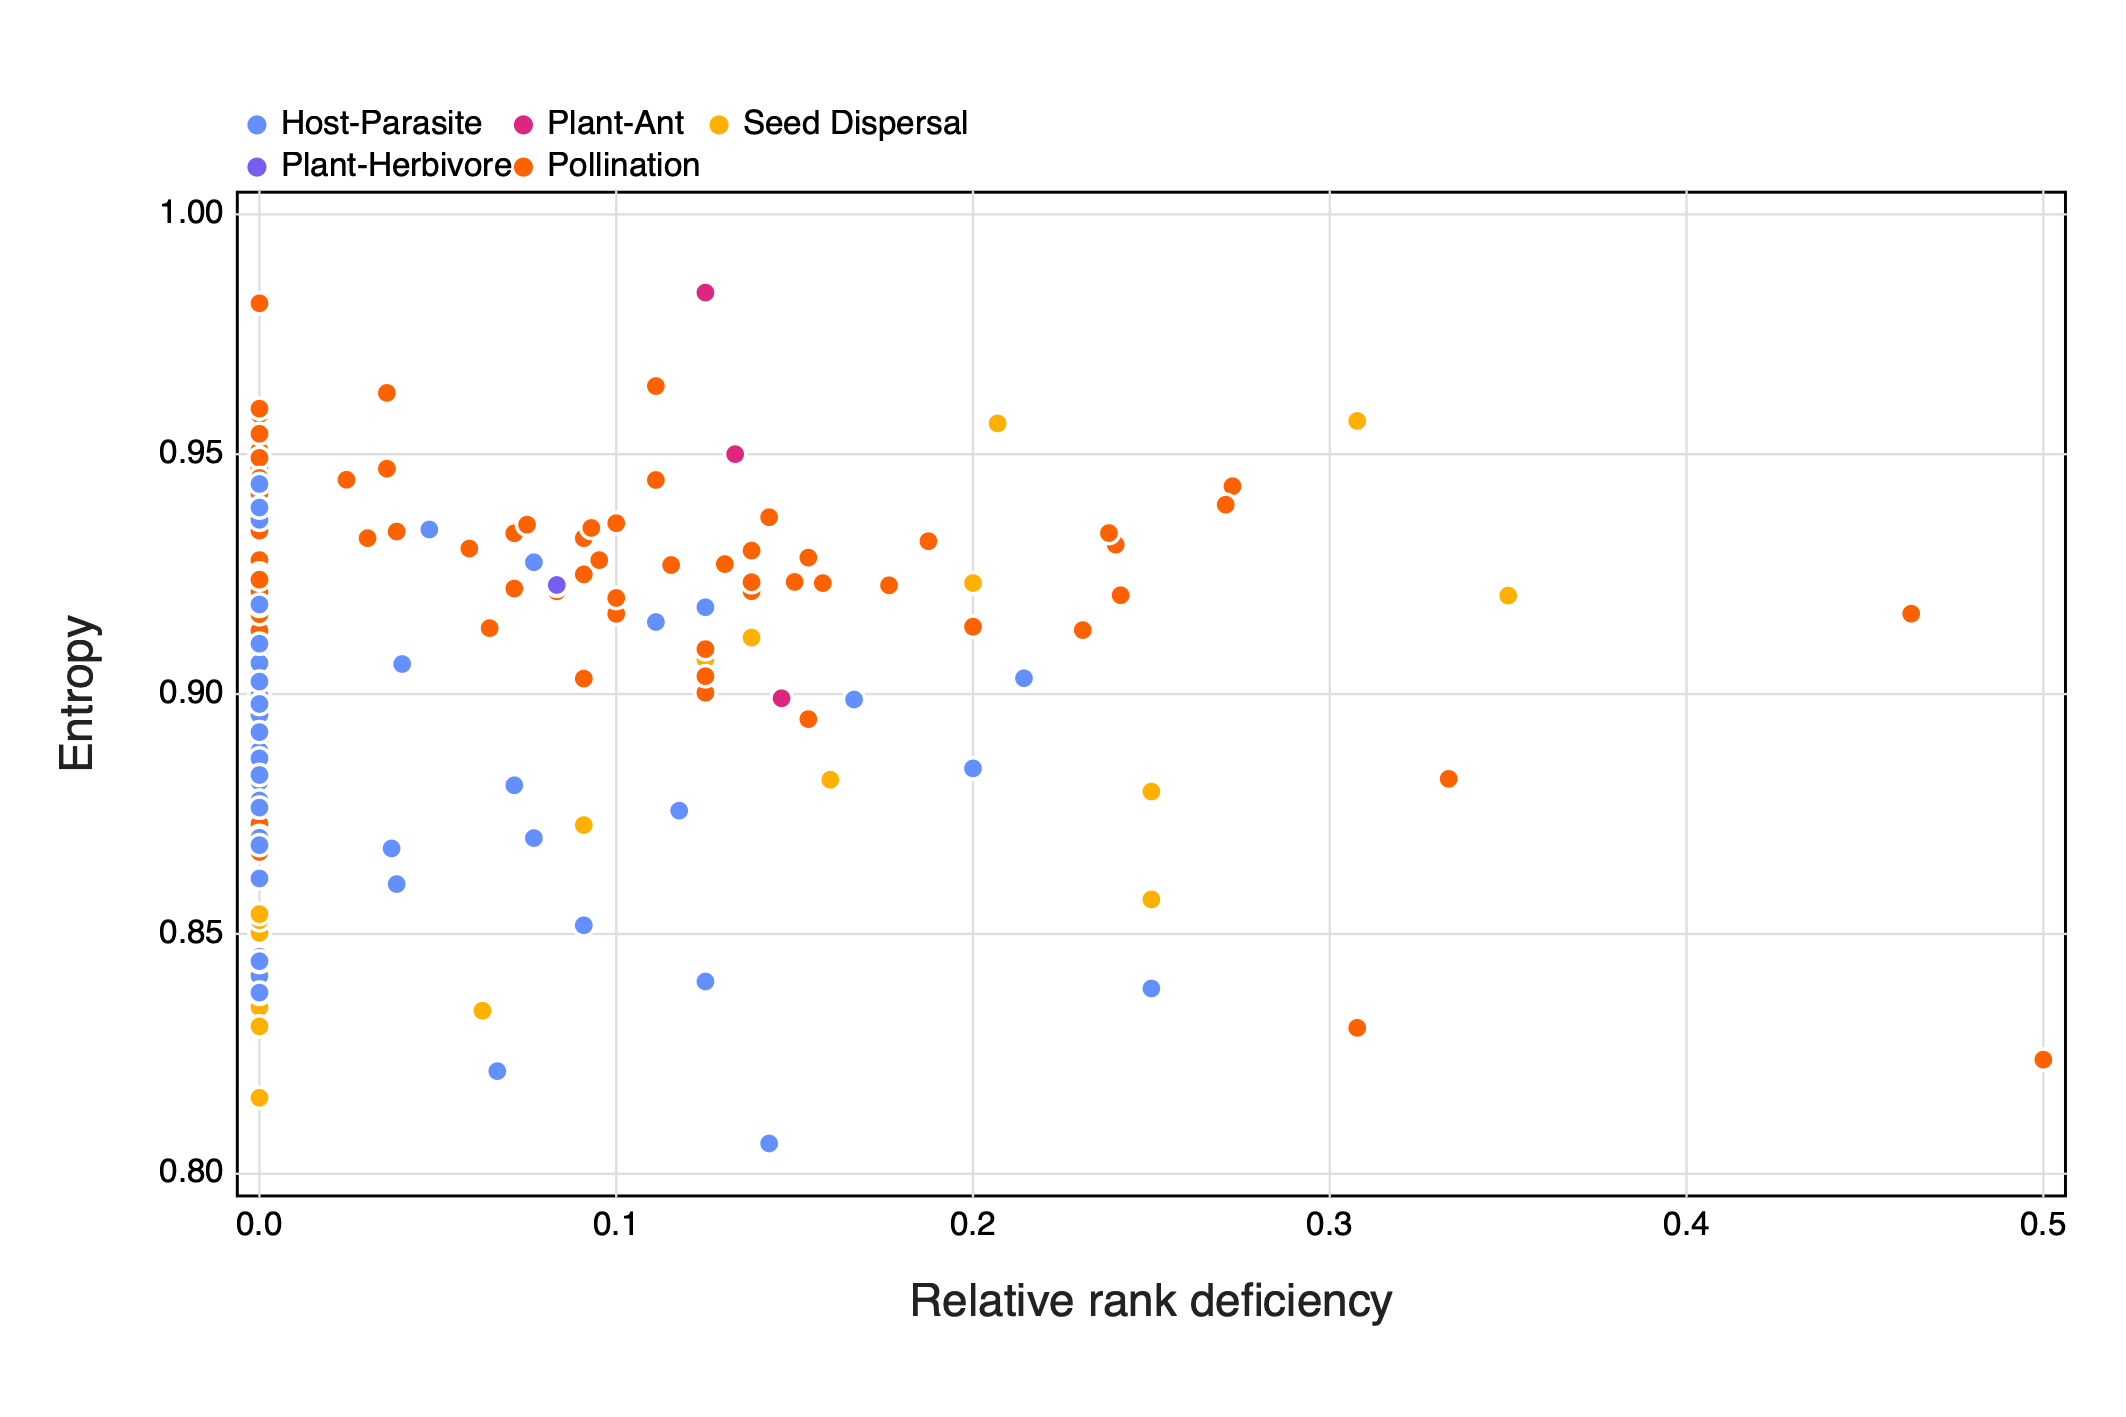
\includegraphics[width=\textwidth]{figures/entropy_v_rank.png}
    \caption{The relationship between SVD entropy and the relative rank
deficiency of different species interaction networks Colours indicate the
different interaction types of the networks.}
    \label{fig:entropy_v_rank}
\end{figure}

\subsection{Most elements of network structure capture network
complexity}\label{most-elements-of-network-structure-capture-network-complexity}

We compared SVD entropy to some of the more common measures of complexity,
namely nestedness (\(\eta\), as per \cite{Bastolla2009ArcMut}),
connectance (\(\text{Co}\)), and the spectral radius of the network (\(\rho\),
following \cite{Staniczenko2013GhoNes}). All of these measures are
positively correlated, especially over the range of connectances covered by
empirical bipartite ecological networks.

Nestedness is calculated based on the number of interactions shared between
species pairs and is a measure of the degree of overlap between species links
(or strategies) in the community, where larger assemblages are made up of a
subset of smaller ones that share common interactions. Networks with a higher
degree of nestedness could be considered simpler when compared to networks with
a lower degree of nestedness. Connectance is the realised number of interactions
(links) in an ecological network and is calculated as the fraction of the total
number of realised interactions (or links) and the maximum number of possible
interactions in a network (\cite{Martinez1992ConCon}). This has been shown to be a
good estimate of a community's resilience to perturbation
(\cite{Dunne2002NetStr}). The spectral radius of a matrix is the largest absolute
value of its eigenvalues, which, in addition to being presented as a measure of
network complexity has also been suggested as an indicator of the ability of a
system to dampen disturbances (\cite{Phillips2011StrEco}).

We find that SVD entropy has a clear negative relationship with nestedness,
spectral radius, and connectance (\autoref{fig:other}). As in
\autoref{fig:type}, mutualistic networks tend to be more complex, and they also
are both sparser and less nested than other types of networks.
\cite{Bastolla2009ArcMut} give a convincing demonstration that
mutualistic networks are shaped to minimise competition -- this can be done by
avoiding to duplicate overlap in interactions, thereby resulting in a network
that is close to full rank, and with high SVD entropy. Interestingly, \autoref{fig:other} suggests that both nestedness and connectance measure the \emph{lack} of complexity in an ecological network, which contrasts to how they may commonly be viewed (\cite{Landi2018Complexity}).

\begin{figure}[h]
    \centering
    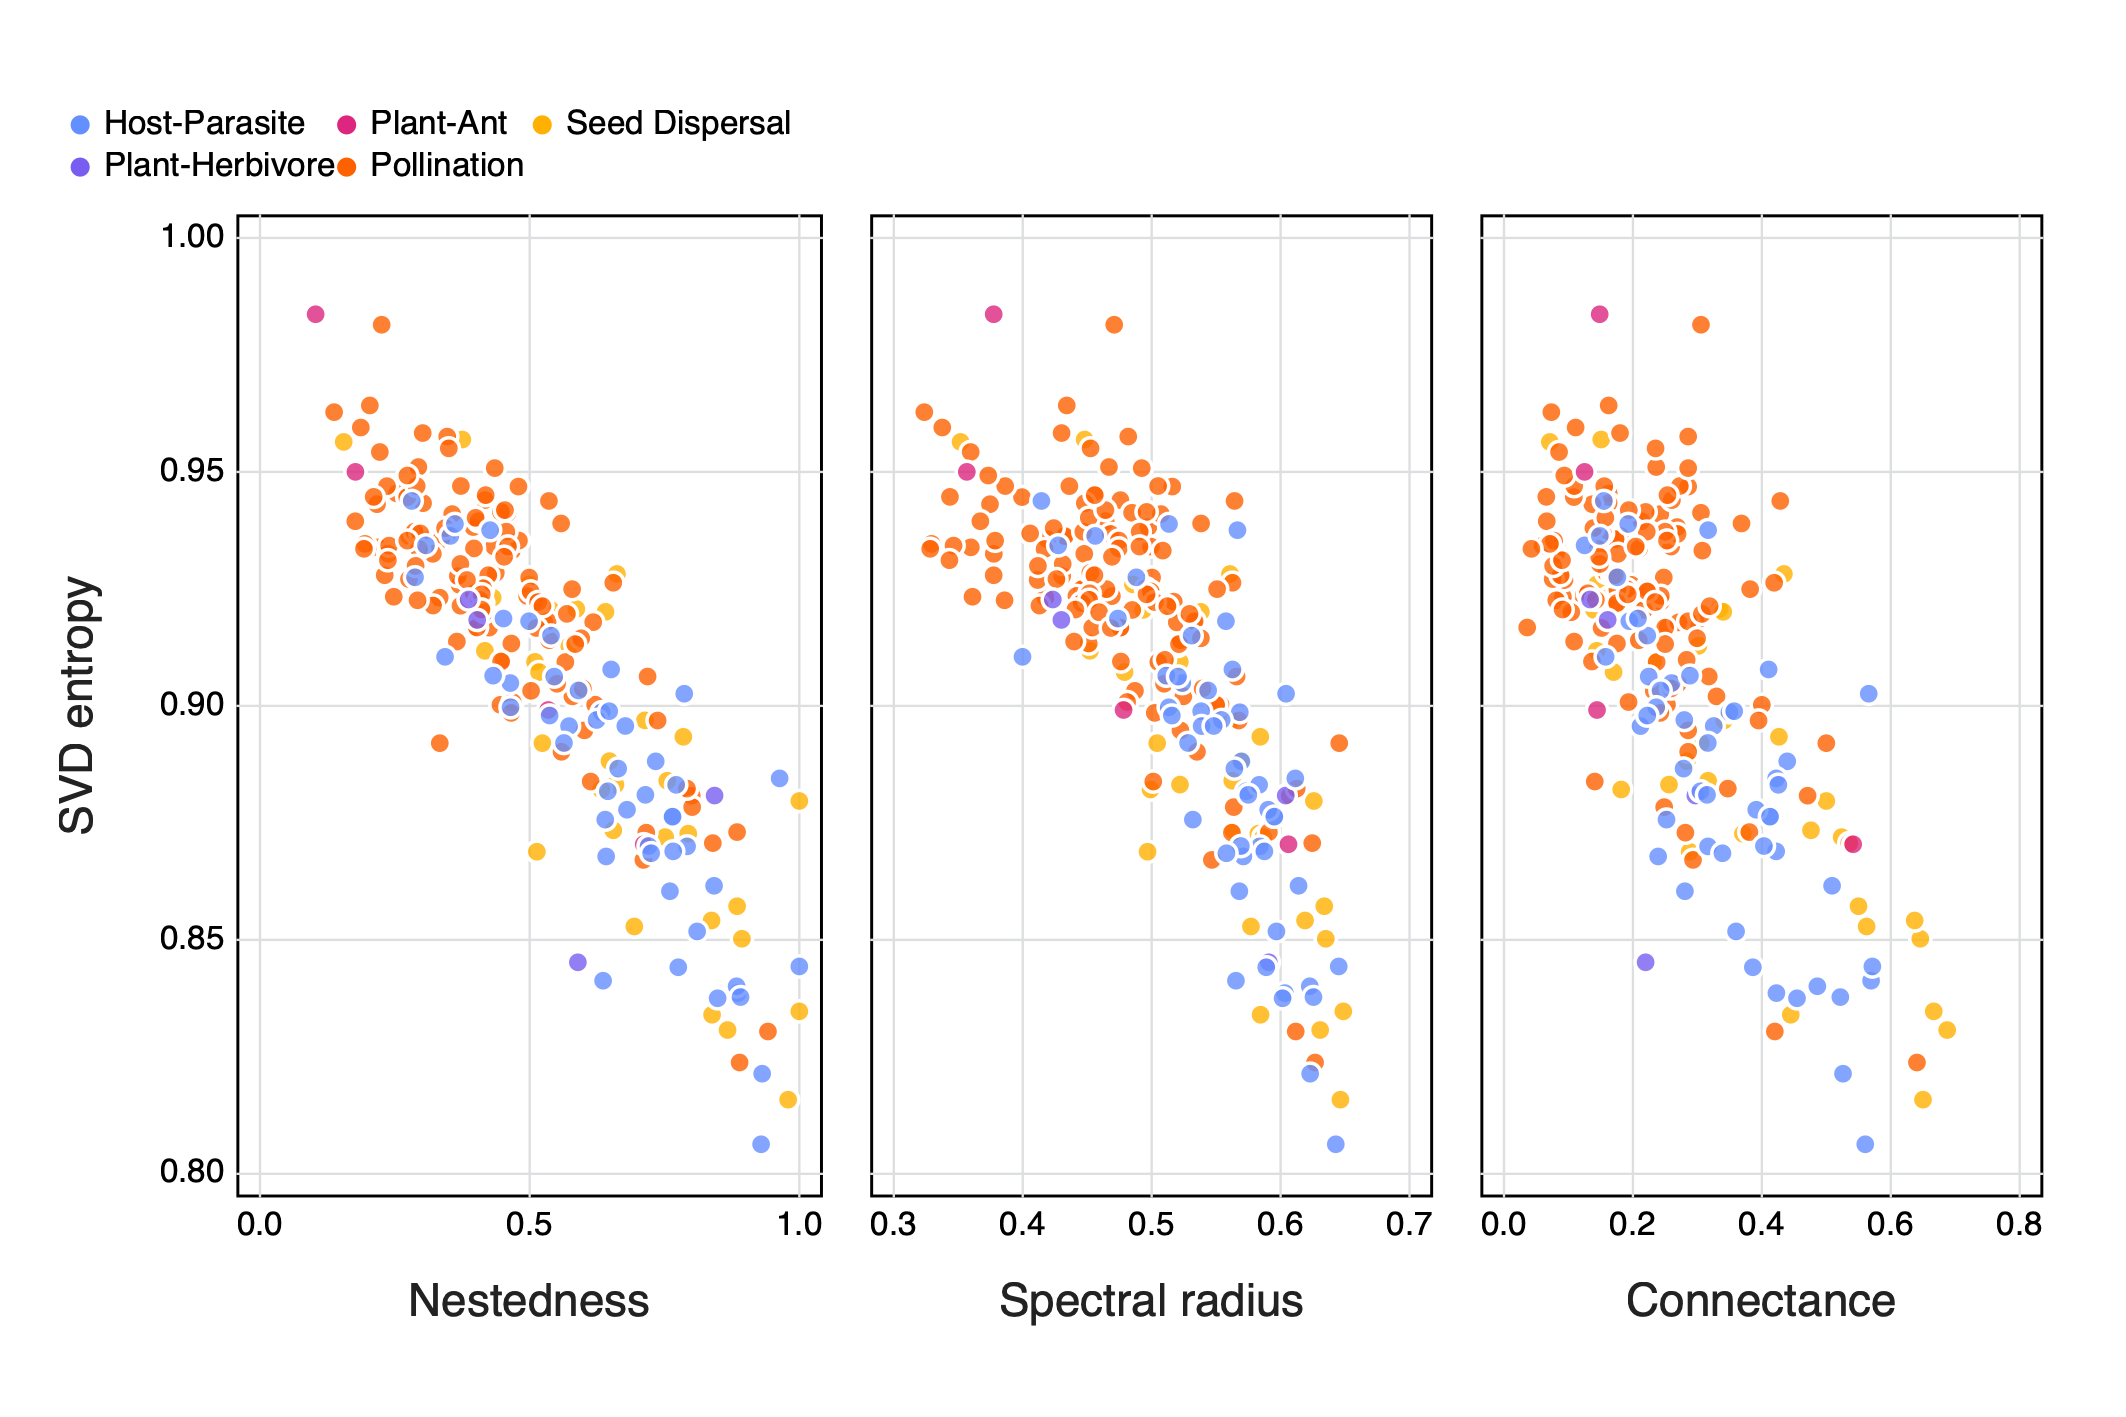
\includegraphics[width=\textwidth]{figures/others_v_entropy.png}
    \caption{The relationship between SVD entropy and the nestedness (left
panel), spectral radius (central panel) and connectance (right panel) of
ecological networks. Colours indicate the different interaction types of the
networks.}
    \label{fig:other}
\end{figure}

\subsection{Complex networks are not more robust to
extinction}\label{complex-networks-are-not-more-robust-to-extinction}

One approach to calculating the overall structural robustness of an ecological
network is by simulating extinction events through the sequential removal of
species, which allows constructing an extinction curve that plots the
relationship between species removed and cumulative secondary extinctions
(\cite{Dunne2002NetStr, Memmott2004TolPol}). Extinction events can be simulated in
a manner of different ways, either by removing 1) a random individual, 2)
systematically removing the most connected species (one with the highest number
of interactions with other species) and 3) the least connected species
(\cite{Dunne2002NetStr}). After each extinction event, we remove species from the
network that no longer have any interacting partners, thereby simulating
secondary extinctions. This is then repeated until there are no species
remaining in the network. Furthermore, we can restrict extinction events to only
one dimension of the interaction matrix, \emph{i.e.,} removing only top-level or
bottom-level species, or alternatively removing a species from any dimension of
the matrix. Extinction curves are then constructed by plotting the proportion of
species remaining against those that have been removed; it stands to reason that
a flatter curve `maintains' its species pool for a longer number of cumulative
extinctions, and could be seen as more resilient, when compared to a curve that
has a much steeper decline. As per previous studies, we measure the robustness
to extinction as the area under the extinction curve (AUC), calculated using the
Trapezoidal rule. AUC values close to 0 means that a single extinction is enough
to collapse the network almost entirely, and values close to 1 means that most
species persist even when the number of extinctions is really high.

When looking at the relationship between SVD entropy and the area under an
extinction curve (as a proxy for resilience to extinction) we find differences
depending on both the extinction mechanism as well as along which dimension the
species removal occurred (\autoref{fig:resilience}). As a whole we do not
observe any obvious relationships between SVD entropy and resilience, nor for
different interaction types. We do however see differences in the resilience of
networks depending on how the extinctions were simulated. Generally we see a
higher resilience in networks where species of only a specific group are removed
or in networks where species were either randomly removed or based on an
increasing number of interactions.

\begin{figure}[h]
    \centering
    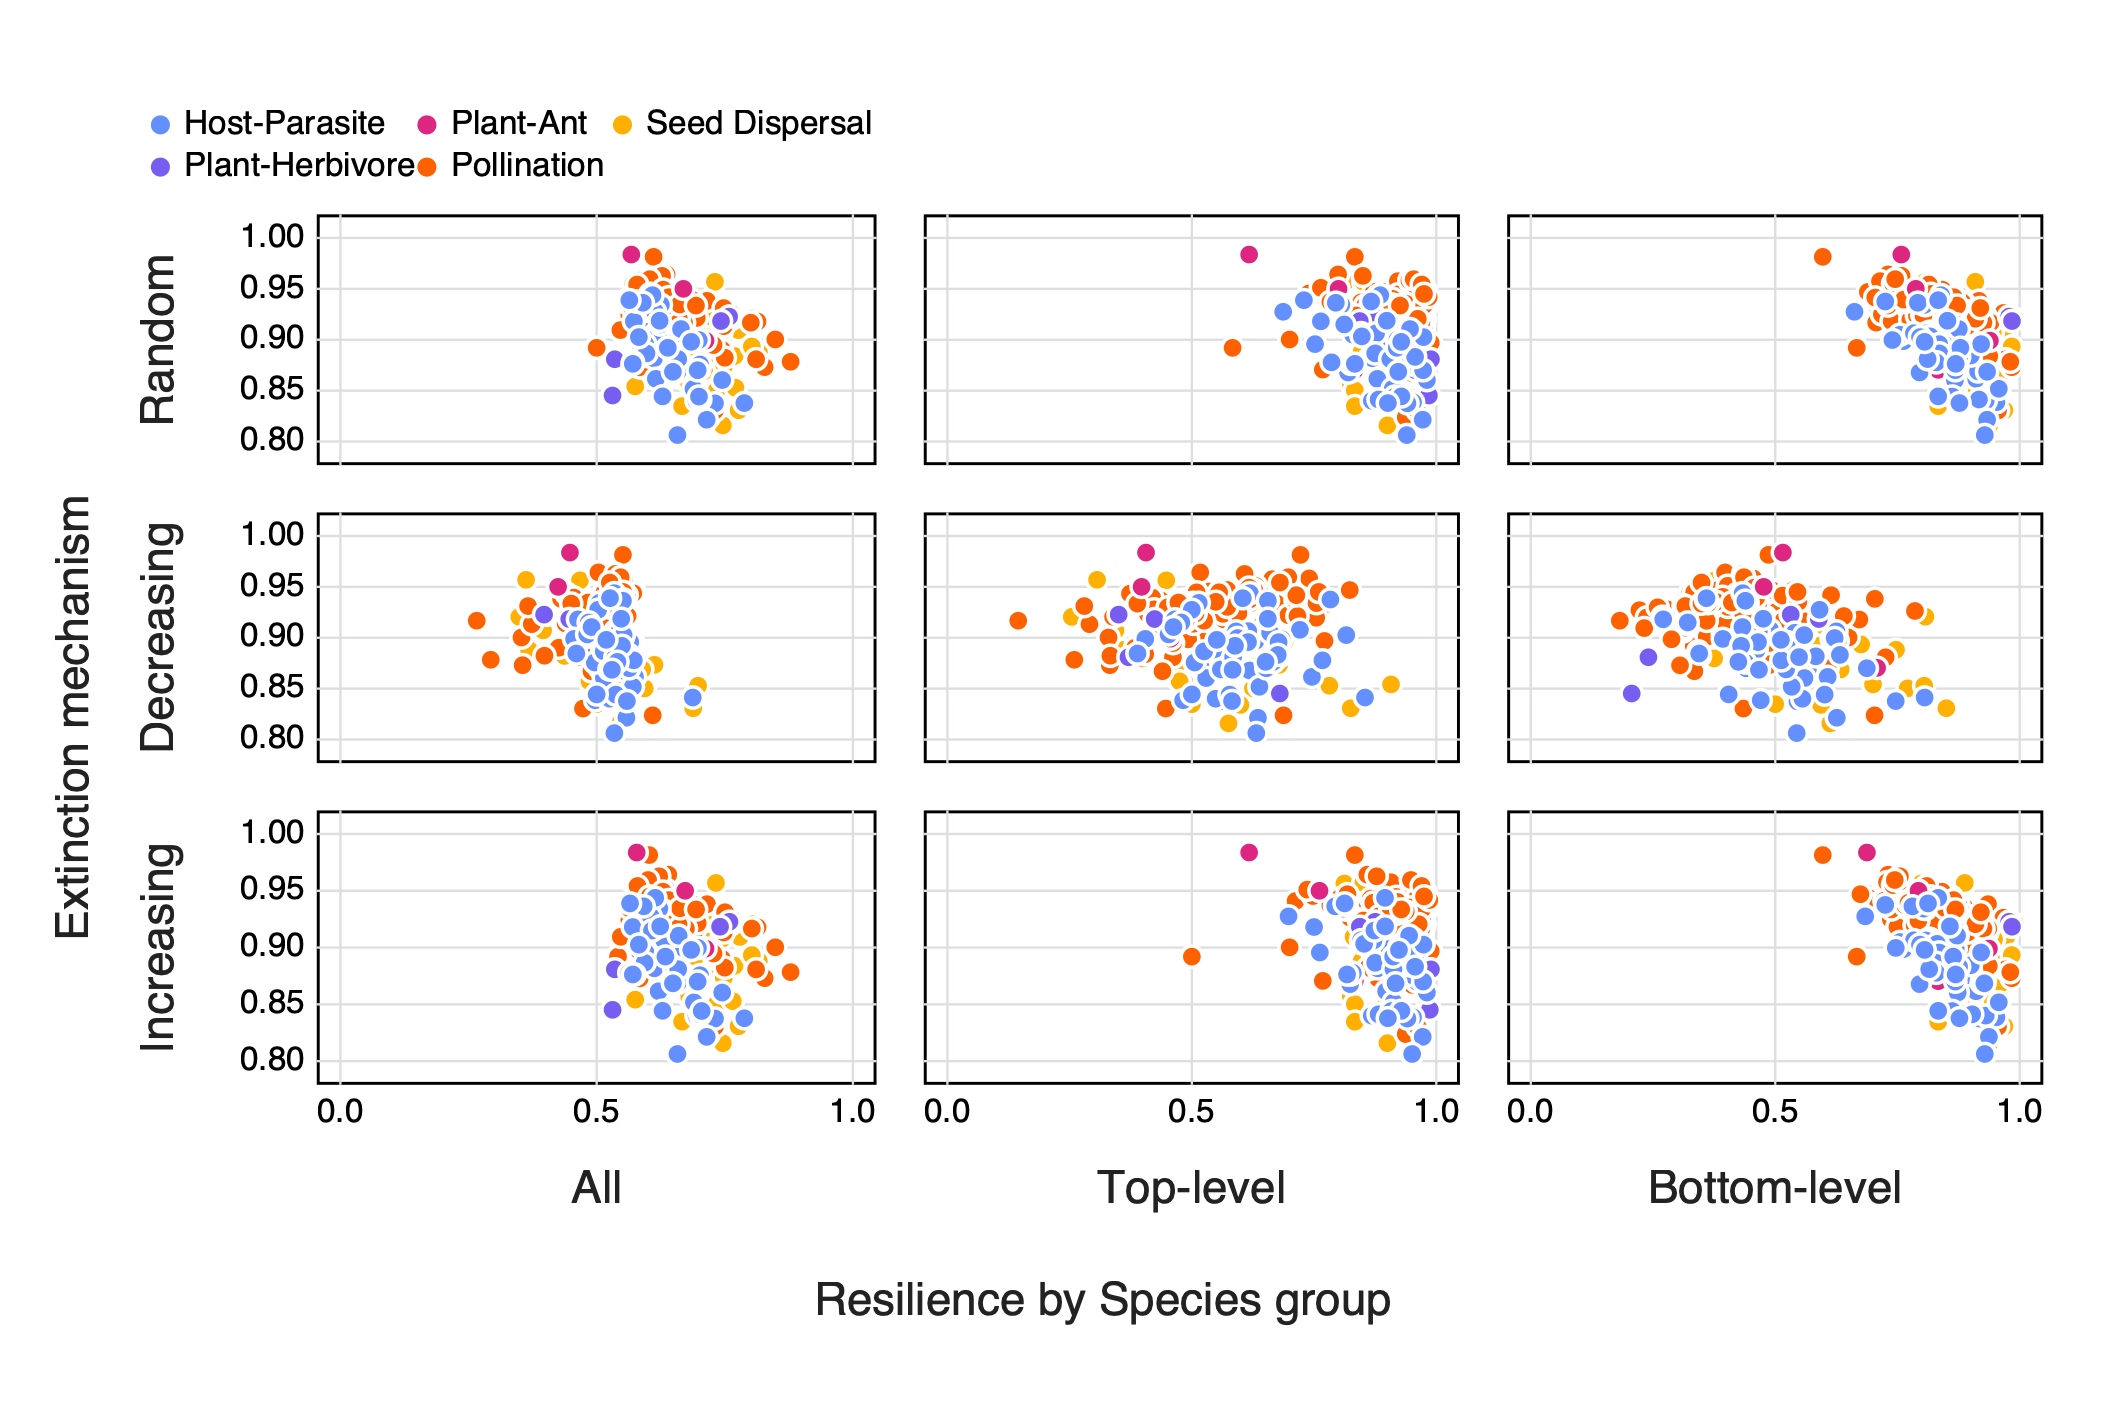
\includegraphics[width=\textwidth]{figures/entropy_v_AUCall.png}
    \caption{The relationship between SVD entropy and the area under an
extinction curve (as a proxy for resilience to extinction) for both different
extinction mechanisms (Random = the removal of a random species, Decreasing =
the removal of species in order of decreasing number of interactions (i.e most
to least number of interactions), Increasing = the removal of species in order
of increasing number of interactions) as well as along different dimensions
(species groups) of the network (All = any species, Top-level = only top-level
species, and Bottom-level = only bottom- level species) Colours indicate the
different interaction types of the networks.}
    \label{fig:resilience}
\end{figure}

As highlighted in \autoref{fig:other} SVD entropy can be used as an additional
measure of network complexity. However, as shown in \autoref{fig:resilience}, the
assumption that network complexity begets resilience to extinction begins to
unravel when we use a measure of physical complexity. This is in contrast to
previous studies that have shown how connectance plays a role in the resilience
of networks to extinctions (\cite{Dunne2002NetStr, Memmott2004TolPol}). This does
not discount the role of using \emph{structural} measures of network complexity
(\emph{e.g.,} connectance, nestedness or spectral radius) as indicators of their
resilience (although possibly hinting as to why there is no strong emerging
consensus as to how structural complexity relates to this), but rather points to
an erroneous assumption as to what aspects of a network we have previously used
to define its complexity.

\subsection{Plant-pollinator networks are slightly more
complex}\label{plant-pollinator-networks-are-slightly-more-complex}

Although we don't observe clear differences in the relationship between
different interaction types when comparing amongst various measures of
complexity, we do find that different types of interaction networks have
differing SVD entropy's. When comparing calculated SVD entropy between
interaction types using an ANOVA (after excluding Plant-Ant and Plant-Herbivore
interactions due to their small sample size in our dataset) we find a
significant difference between group means (\(F = 47.047, p < 10^{-3}\)). A
Tukey's HSD test reveals that plant-pollinator networks (\(\mu = .924\)) are
more complex than both host- parasite networks (\(\mu = .885, p < 10^{-3}\)) and
seed dispersal (\(\mu = .888, p < 10^{-3}\)). Host-parasite and seed dispersal
networks had apparently no difference in average complexity (\(p = .889\)).
These results suggest that mutualistic networks may be more complex, which
matches with previous literature: these networks have been shown to minimise
competition (\cite{Bastolla2009ArcMut}) and favour unique interactions, thereby
increasing network complexity. This specific structure can appear as a
side-process of either ecological (\cite{Maynard2018NetSpa}) or evolutionary
(\cite{Valverde2018ArcMut}) processes, but nevertheless leaves a profound imprint
on the complexity of the networks.

\begin{figure}[h]
    \centering
    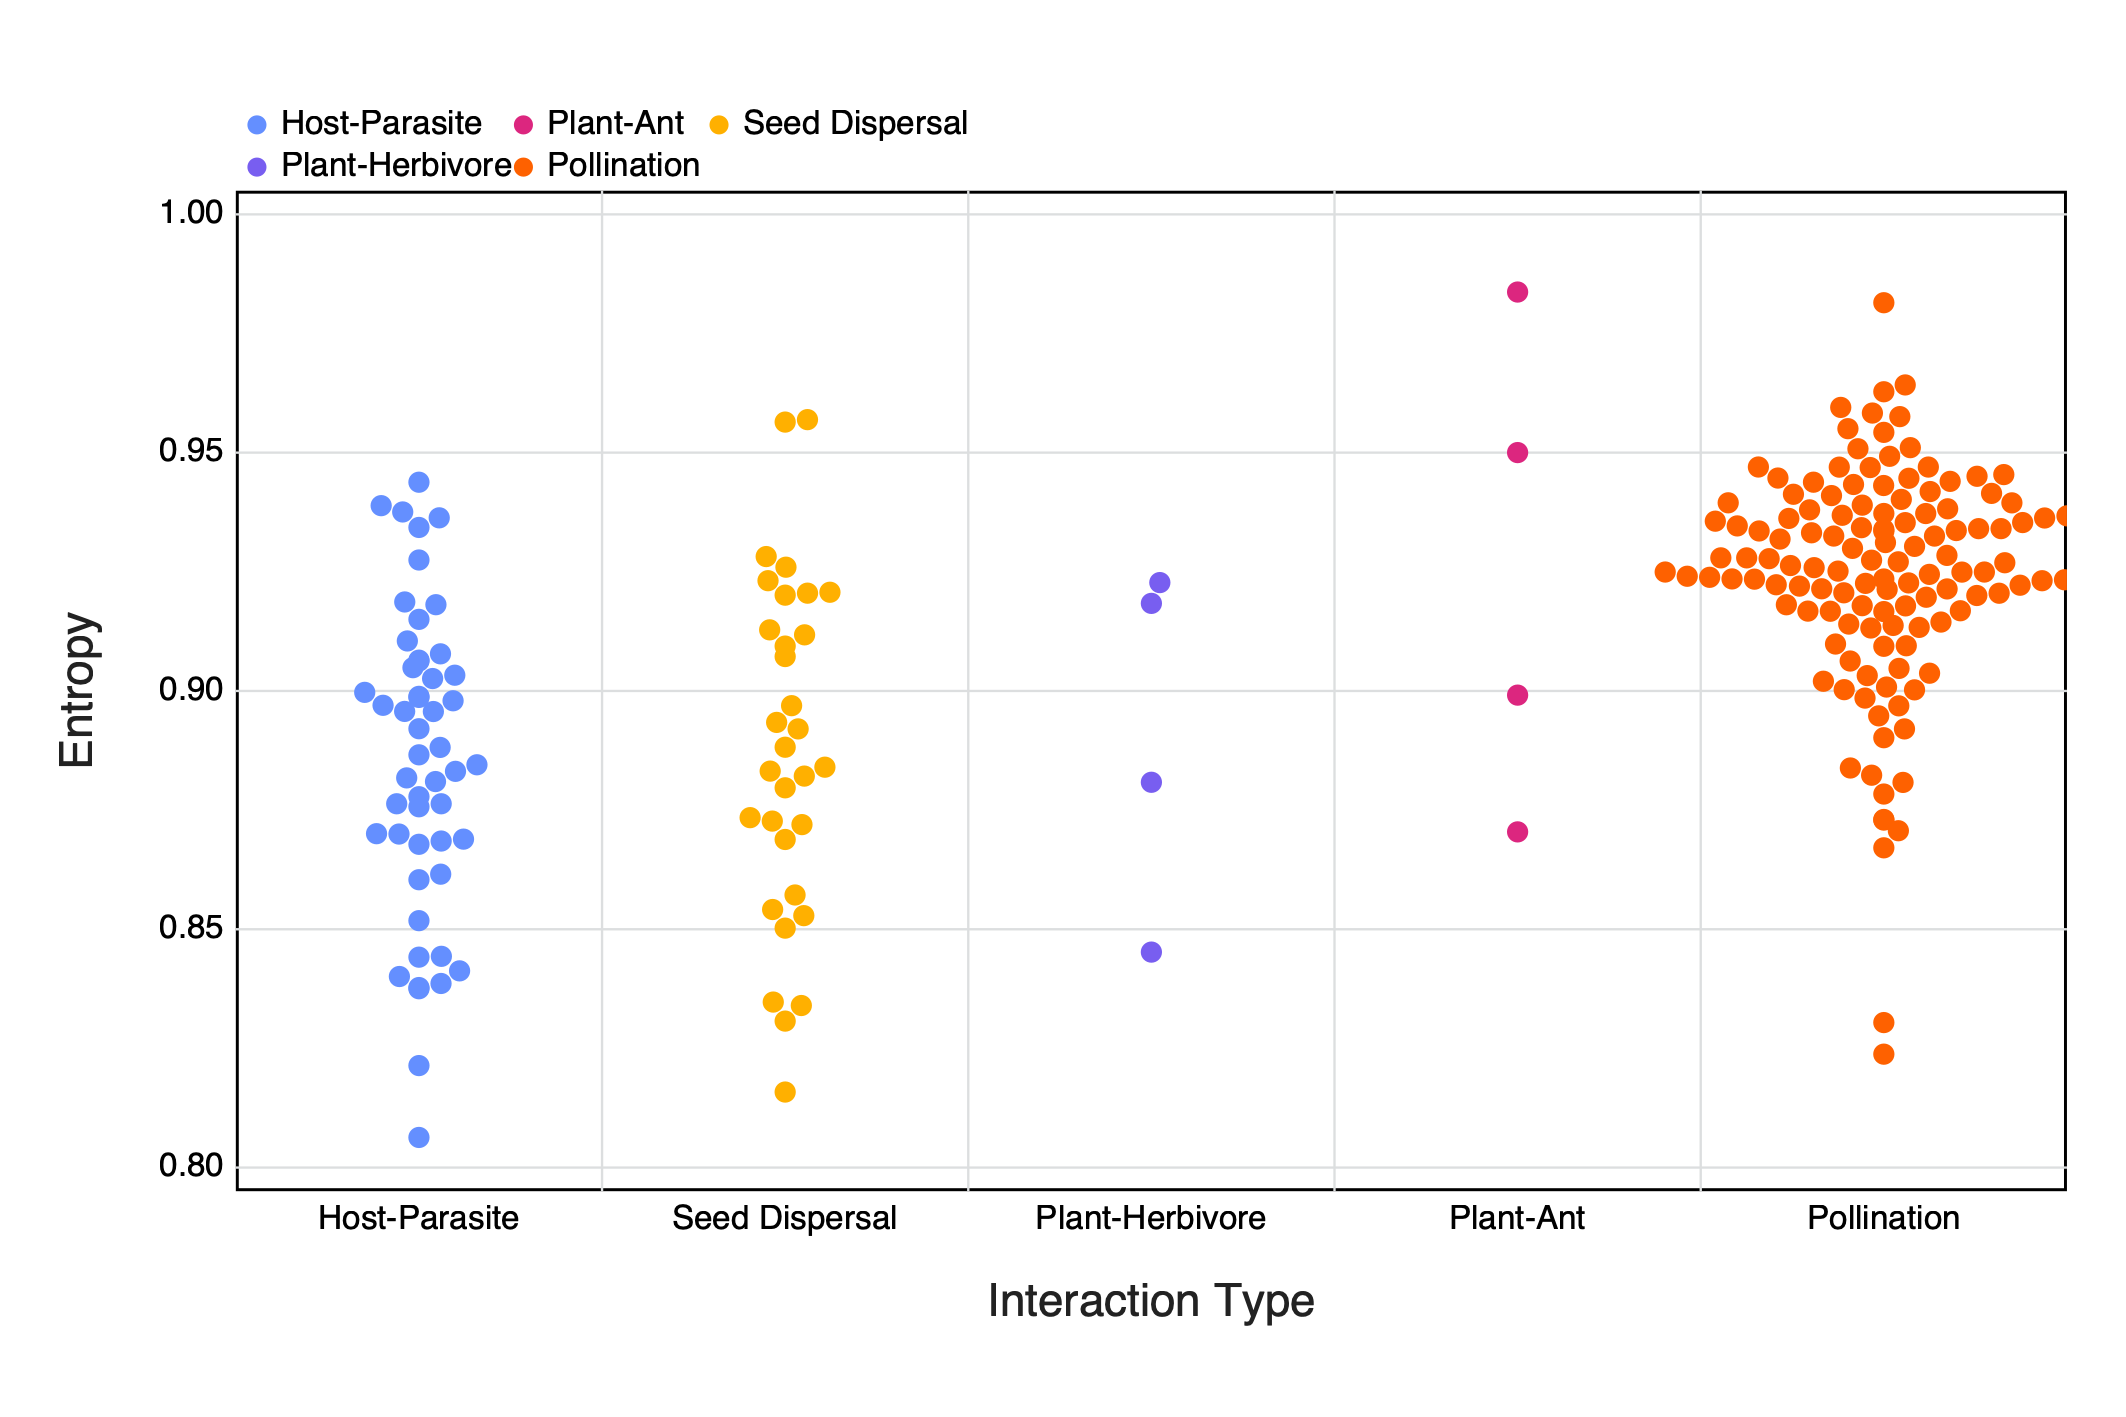
\includegraphics[width=\textwidth]{figures/interactiontype_v_entropy.png}
    \caption{The calculated SVD entropy of different interaction networks of
different interaction types}
    \label{fig:type}
\end{figure}

\subsection{Connectance constrains complexity (but also rank
deficiency)}\label{connectance-constrains-complexity-but-also-rank-deficiency}

We used simulated annealing (\cite{Kirkpatrick1984OptSim}) to generate networks
with the highest, or lowest, possible SVD entropy values. From a set network
size (30 species, 15 on each side) with a random number of interactions
(spanning the entire range from minimally to maximally connected), we
reorganised interactions until the SVD entropy was as close to 0 or 1 as
possible. We repeated the process 25 times for every number of interactions. We
also measured the relative rank deficiency of the generated networks. This
allows identifying the boundaries of both measures of complexity. The specific
simulated annealing we used is as follows. We set an initial temperature \(T_0 =
2\). At every timestep \(t\) (up until \(t = 10^4\)), the temperature is set to
\(T_t = T_0\times\lambda^t\), so that is decays exponentially at a rate
\(\lambda = 1 - 10^{-4}\). At each timestep, we switch two interactions in the
network \(\mathcal{N}\) at random to generate a proposal network
\(\mathcal{M}\). The score of this proposal is the difference between the
squared error of \(\mathcal{N}\) and \(\mathcal{M}\) \emph{i.e.,} \(\Delta =
(f(\mathcal{M})-\theta)^2-(f(\mathcal{N})-\theta)^2\), where \(f\) is the SVD
entropy and \(\theta\) is the target for optimisation (either 0 or 1 for
respectively minimally or maximally complex). A proposal is accepted with
probability \(\text{P}(\mathcal{N} \rightarrow \mathcal{M} | \Delta) =
\text{exp}\left(-\Delta\times T_t^{-1}\right)\).

By exploring the minimal and maximal values of SVD entropy for networks of a
given size, we can show that the range of complexity that a network can express
varies as a function of connectance (\autoref{fig:simann}). As reported by
\cite{Poisot2014WheEco}, there is no variation when the networks are
either minimally or maximally connected, but any connectance in between can give
rise to networks of varying complexities. This being said -- minimally connected
networks always show the largest complexity, and an increase in connectance will
always decrease complexity. Interestingly, this relationship is monotonous, and
there is no peak of complexity where the maximal number of possible networks
combination exists, \emph{i.e.,} around \(\text{Co} \approx 0.5\)
(\cite{Poisot2014WheEco}). This is an intriguing result -- ecological networks are
indeed extremely complex, but whereas ecologists have usually interpreted
connectance as a measure of complexity, it is in fact sparse networks that are
the complex ones, and connectance acts to decomplexify network structure.

\begin{figure}[h]
    \centering
    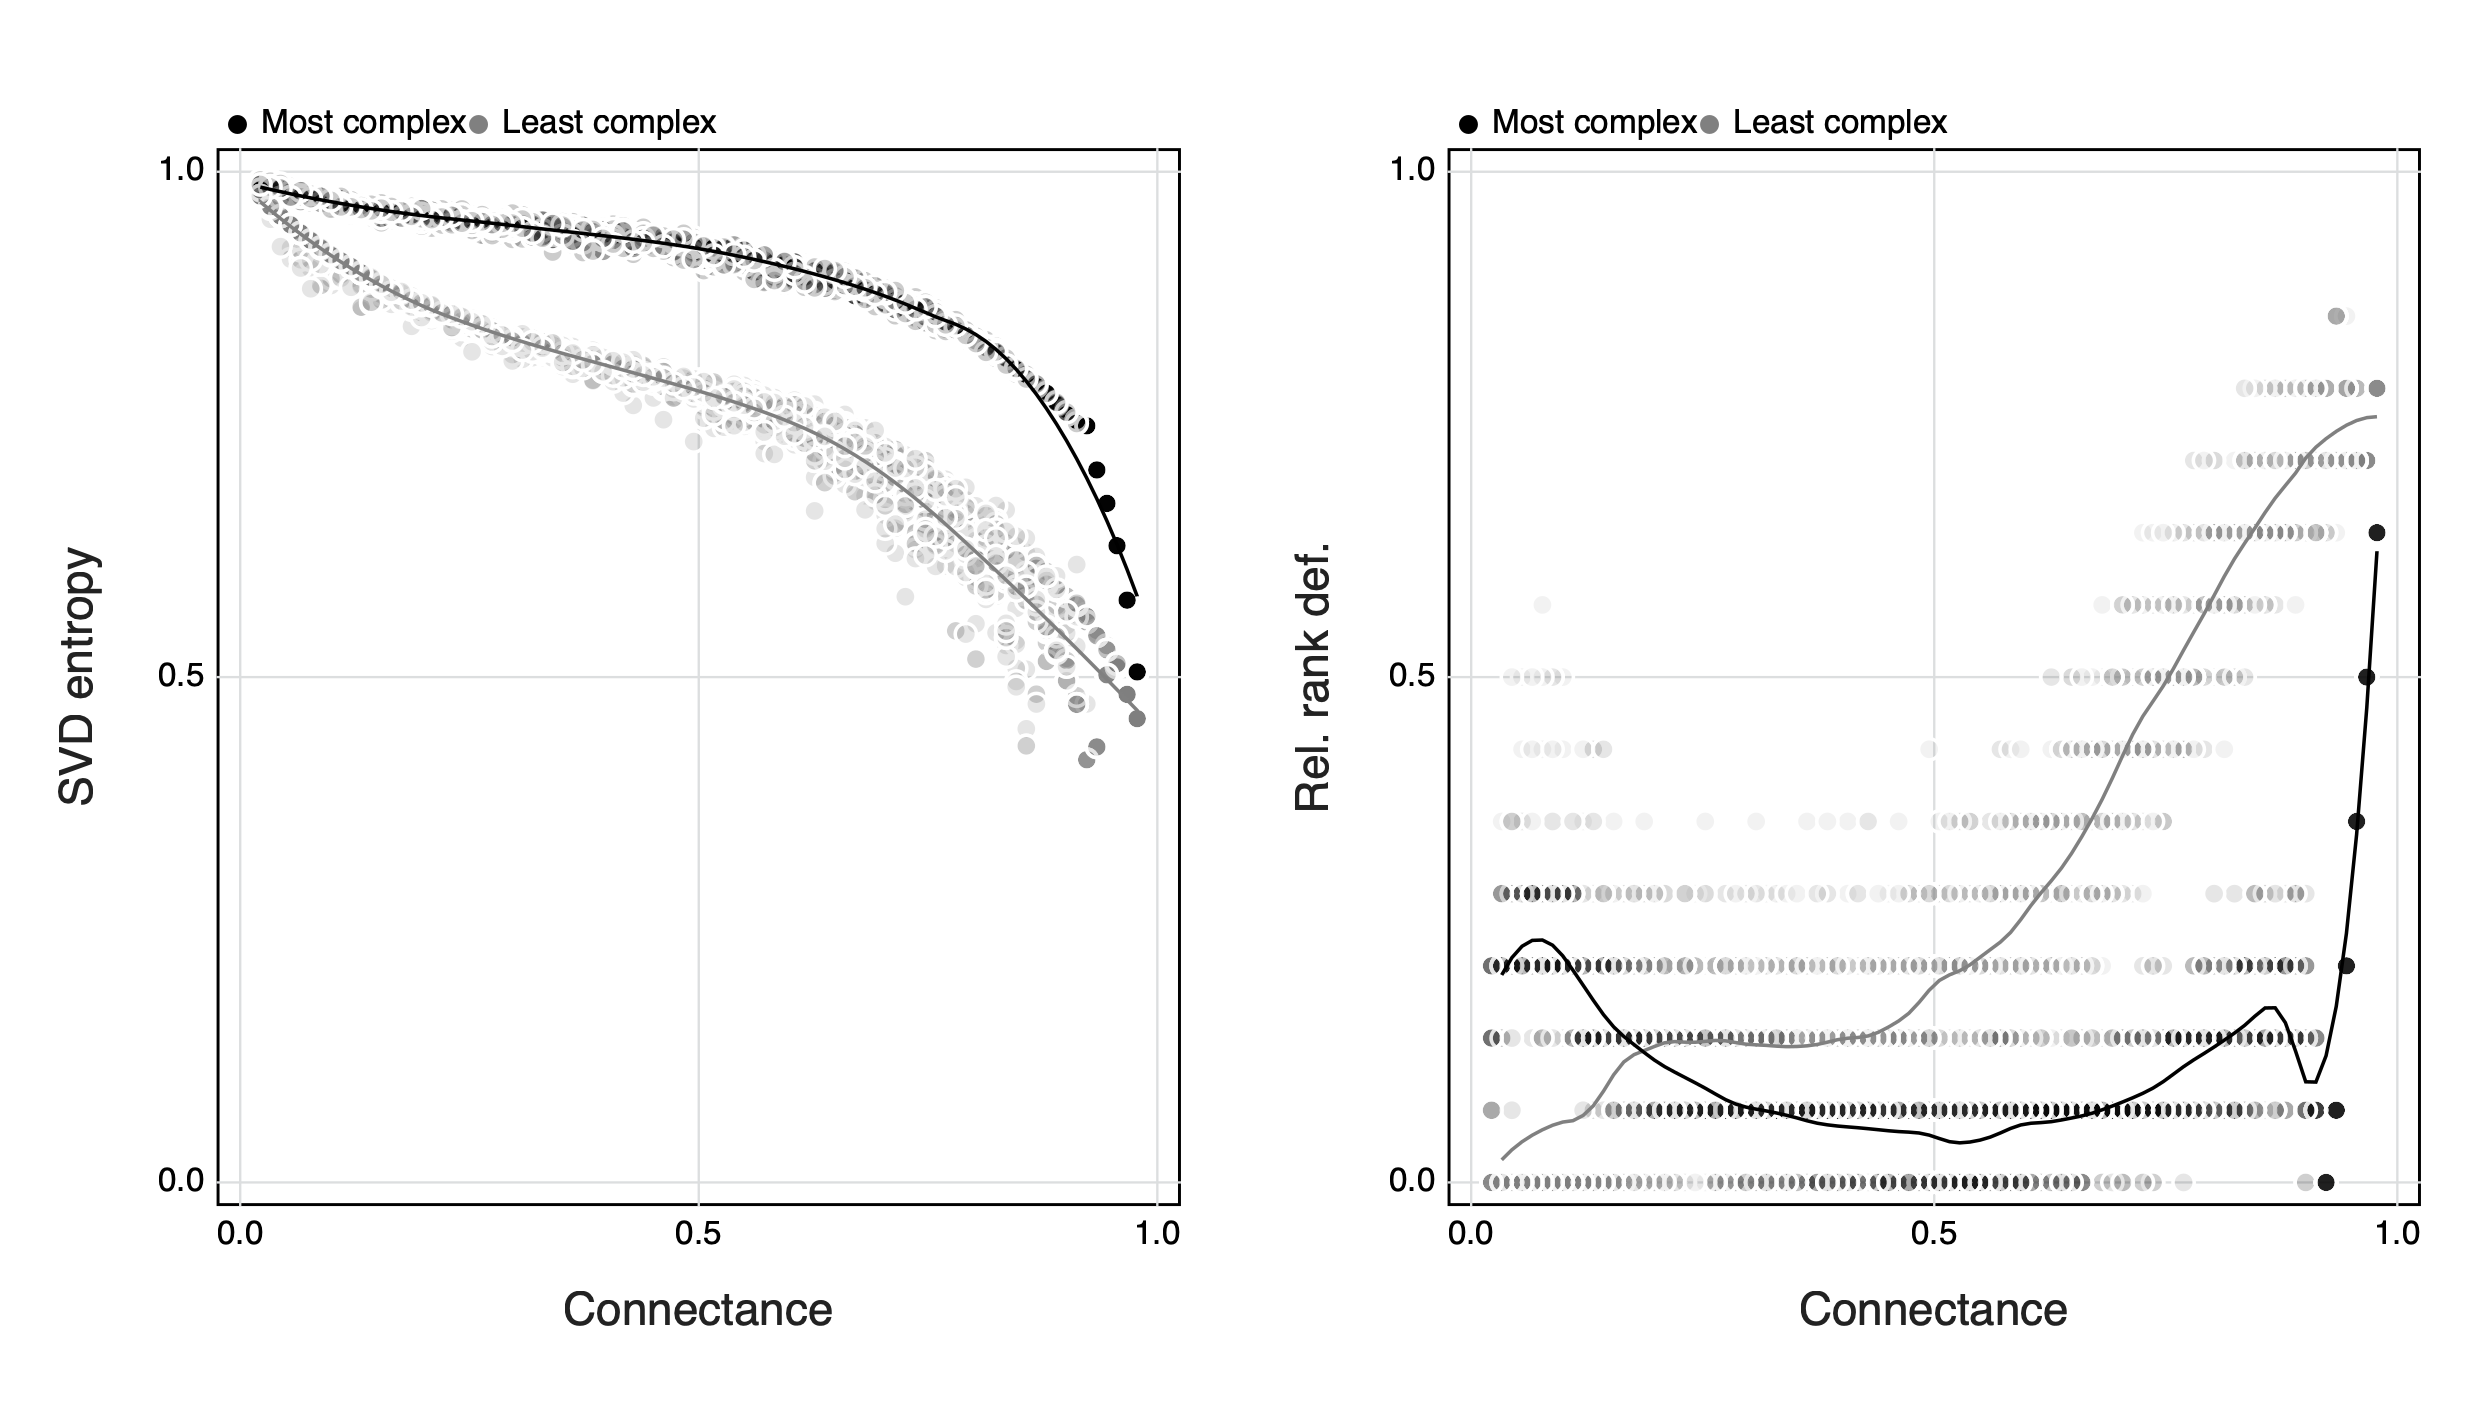
\includegraphics[width=\textwidth]{figures/minmax_combined.png}
    \caption{The relationship between the maximum and minimum value of SVD
entropy of a collection of random interaction networks (using simulated
annealing) for a given connectance spanning from 0 to 1 (left panel) and how
this relates to the relative rank deficiency of networks (right panel)}
    \label{fig:simann}
\end{figure}

The right panel of \autoref{fig:simann} shows the average rank deficiency of
networks for which SVD entropy was either maximised or minimised. Complex
networks (meaning, maximally complex given their connectance) had a lower
deficiency, indicating that except at extreme connectances, there are
combinations of networks for which all species can interact in unique ways --
this is a natural consequence of the results reported by
\cite{Poisot2014WheEco}, whereby the number of possible networks is only
really constrained at the far ends of the connectance gradient. Minimally
complex networks, on the other hand, saw their rank deficiency increase with
connectance. This hints at the fact that the decrease in complexity with
connectance may be primarily driven by the infeasibility of having enough
species for them to all interact uniquely as connectance increases. Because
non-unique interactions tend to result in competition
\cite{Bascompte2007PlaMut}, this can ``push'' networks towards the full-rank
configuration (as suggested by the results in \autoref{fig:size}), thereby
maximising complexity regardless of connectance.

\subsection{Larger networks are less complex than they could
be}\label{larger-networks-are-less-complex-than-they-could-be}

To assess whether ecological networks are more, or less, complex than expected,
we applied two null models that generate pseudo-random networks: Type I
(\cite{Fortuna2006HabLos}), where interactions happen proportionally to
connectance, and Type II (\cite{Bascompte2003Nested}), where interactions happen
proportionally to the joint degree of the two species involved. The models are
equivalent to, respectively, the Erdos-Renyi and Configuration models
(\cite{Newman2010NetInt}), both of which are maximum entropy generative models
that reflect global (Type I) or local (Type II) constraints
(\cite{Park2004Statistical}). We generated 999 samples for every network in the
dataset, and measured the \emph{z}-score of the empirical network as

\[z_i = \frac{x_i-\mu_i}{\sigma_i}\]\

where \(x_i\) is the SVD entropy of network \(i\), and \(\mu_i\) and
\(\sigma_i\) are respectively the average and standard deviation of the
distribution of SVD entropy under the null model. Negative values of \(z_i\)
reflect a network that has lower entropy than expected under the assumptions of
the null model. In \autoref{fig:nullmod}, we show that despite high
\emph{absolute} values of SVD entropy, ecological networks are not as complex as
they \emph{could} be. This is consistently true for both null models, and for
the three types of networks that had a sufficient sample size.

\begin{figure}[h]
    \centering
    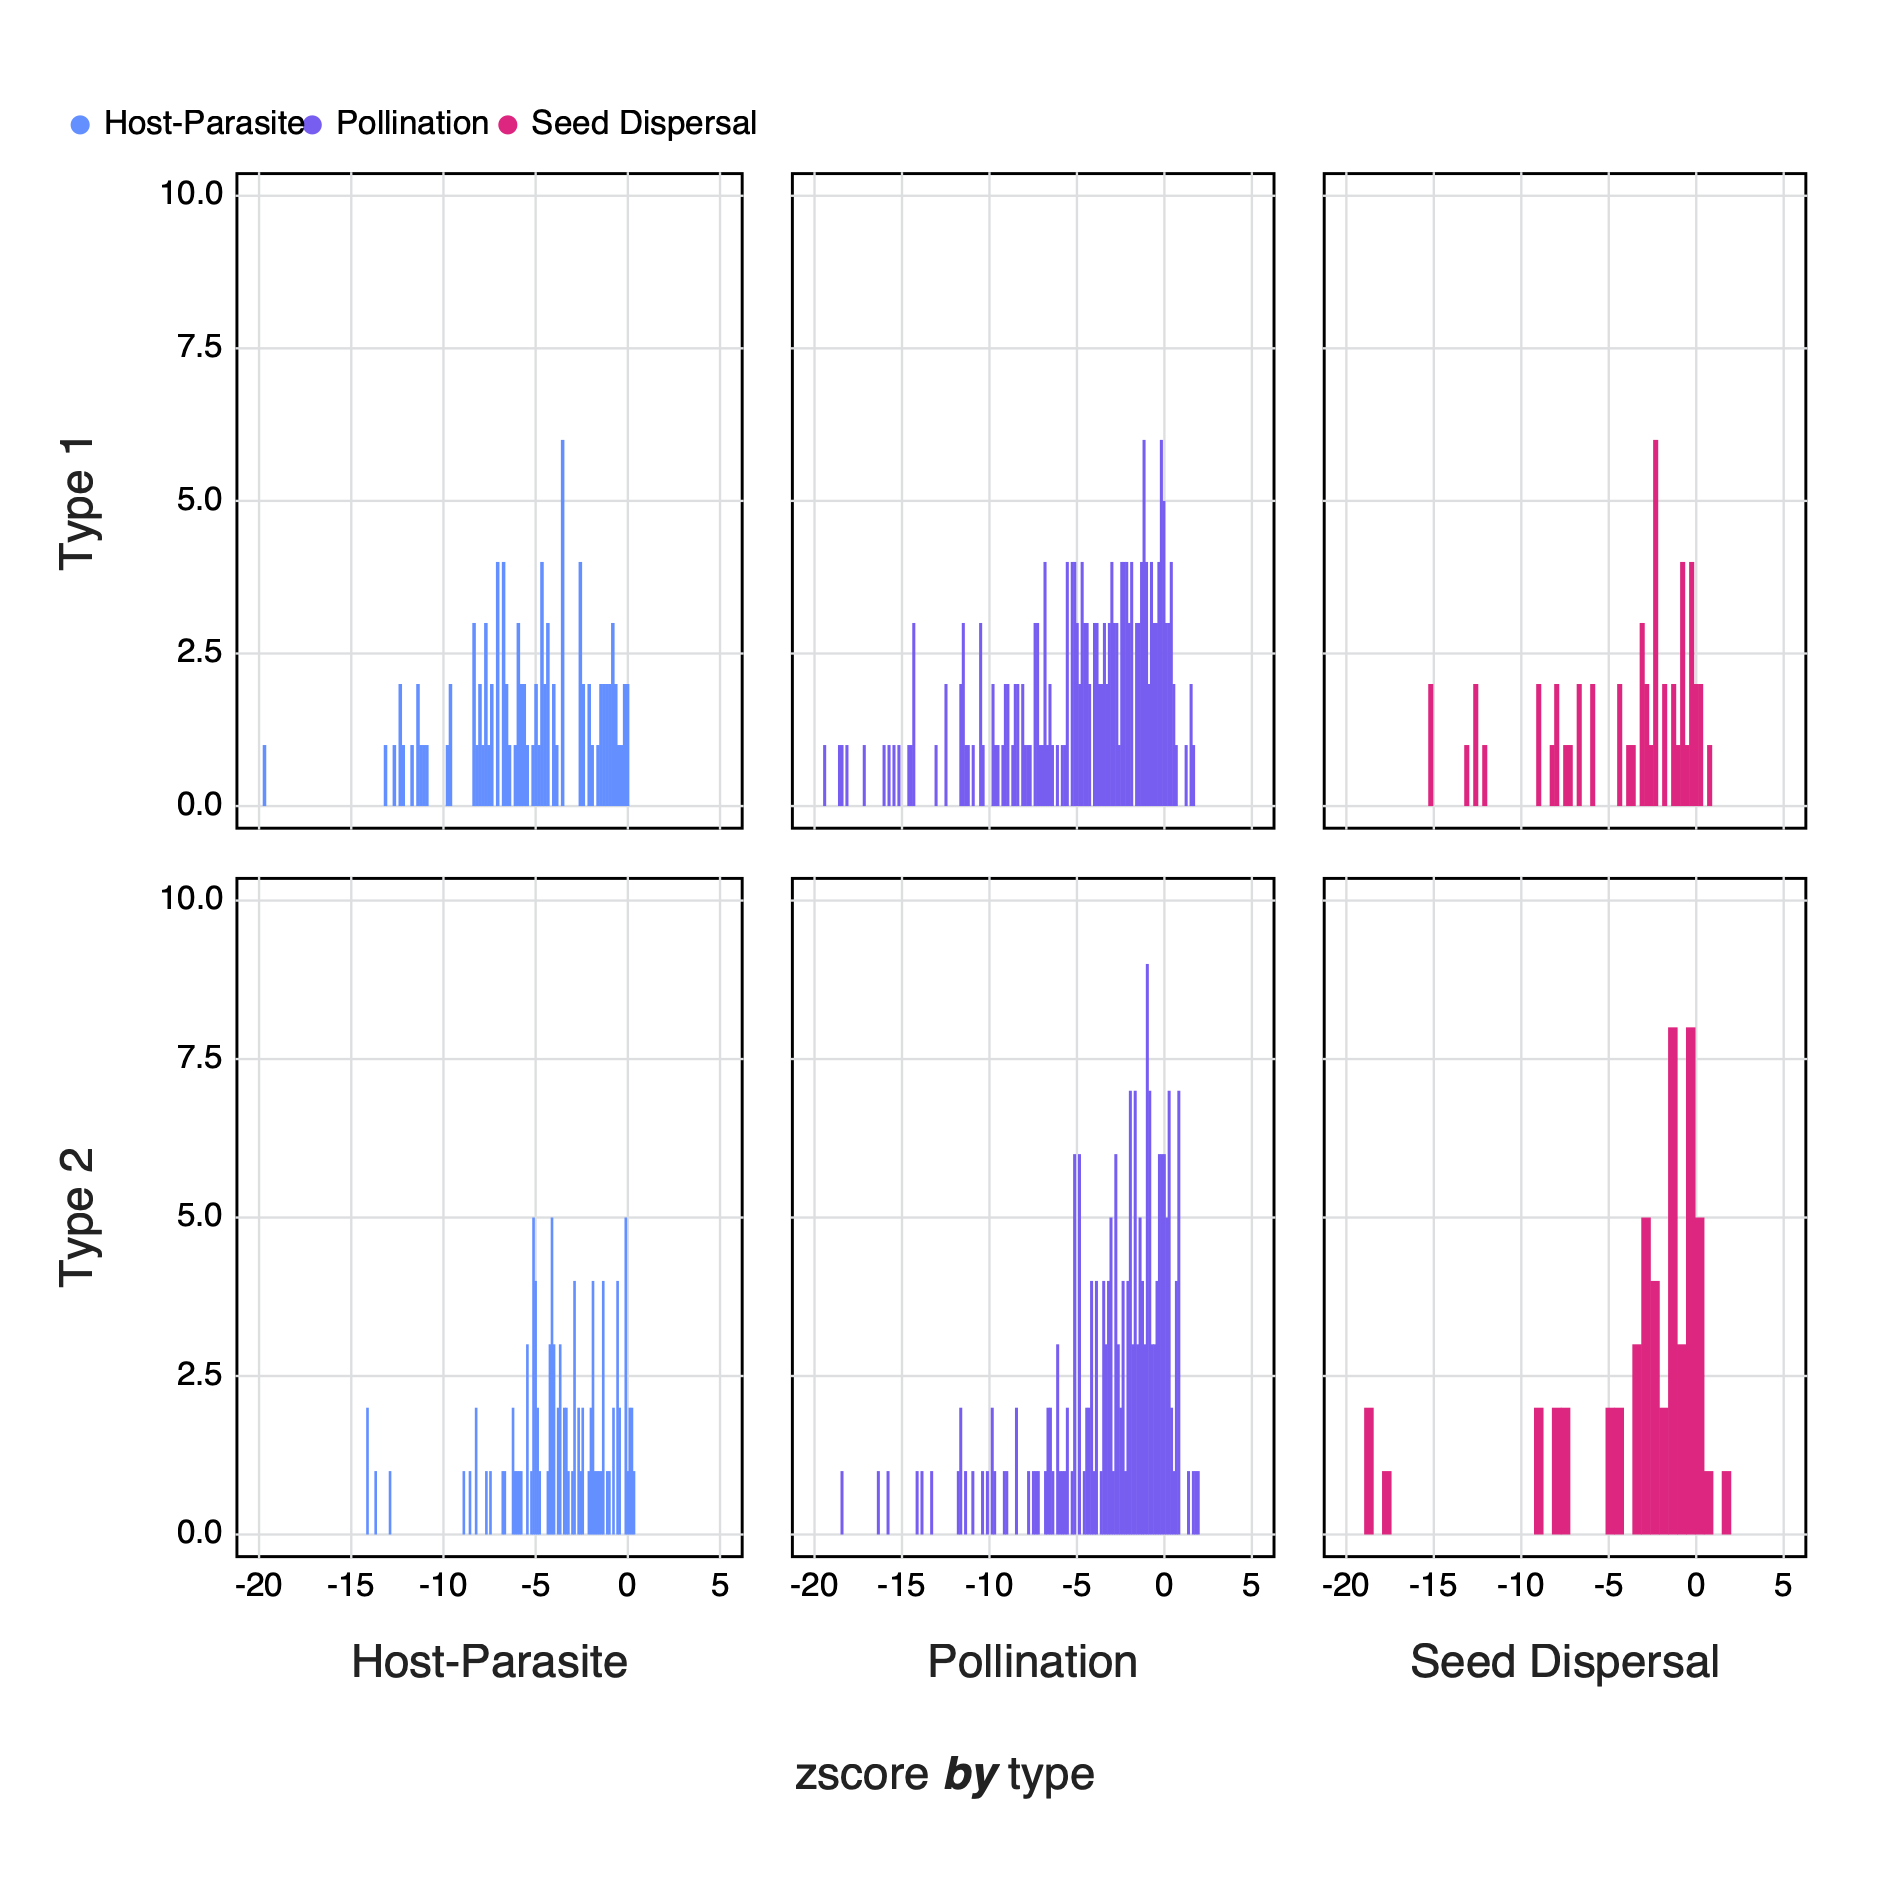
\includegraphics[width=\textwidth]{figures/nullmodel_histogram.png}
    \caption{The counts of the \(z_i\)-scores of different types of networks for
both Type I and Type II null models. Negative \(z_i\)-scores indicate networks
with an SVD entropy that is lower \emph{i.e.,} less complex than expected}
    \label{fig:nullmod}
\end{figure}

Previous work on random networks (using a model that is essentially the Type I
null model) shows that sufficiently large networks achieve maximal von Neuman
entropy (\cite{Du2010NotNeu, Passerini2011NeuEnt}). In \autoref{fig:larger}, we compare the
\emph{logistic} of \(z_i\) to the richness of the network. Transforming to the
logistic smooths out differences in absolute value that are apparent in
\autoref{fig:nullmod}, and projects the values in the unit range, with values
above \(0.5\) being more complex than expected. It is quite obvious that, across
both models and the three types of interactions, only smaller networks achieve
higher entropy. Both \cite{Barbier2018GenAss} and \cite{Saravia2018EcoNet} have previously noted that the early stages of
network assembly usually result in severely constrained networks, due to the
conditions required for multiple species to persist; as networks grow larger,
these constraints may ``relax'', leading in networks with more redundancy, and
therefore a lower complexity.

\begin{figure}[h]
    \centering
    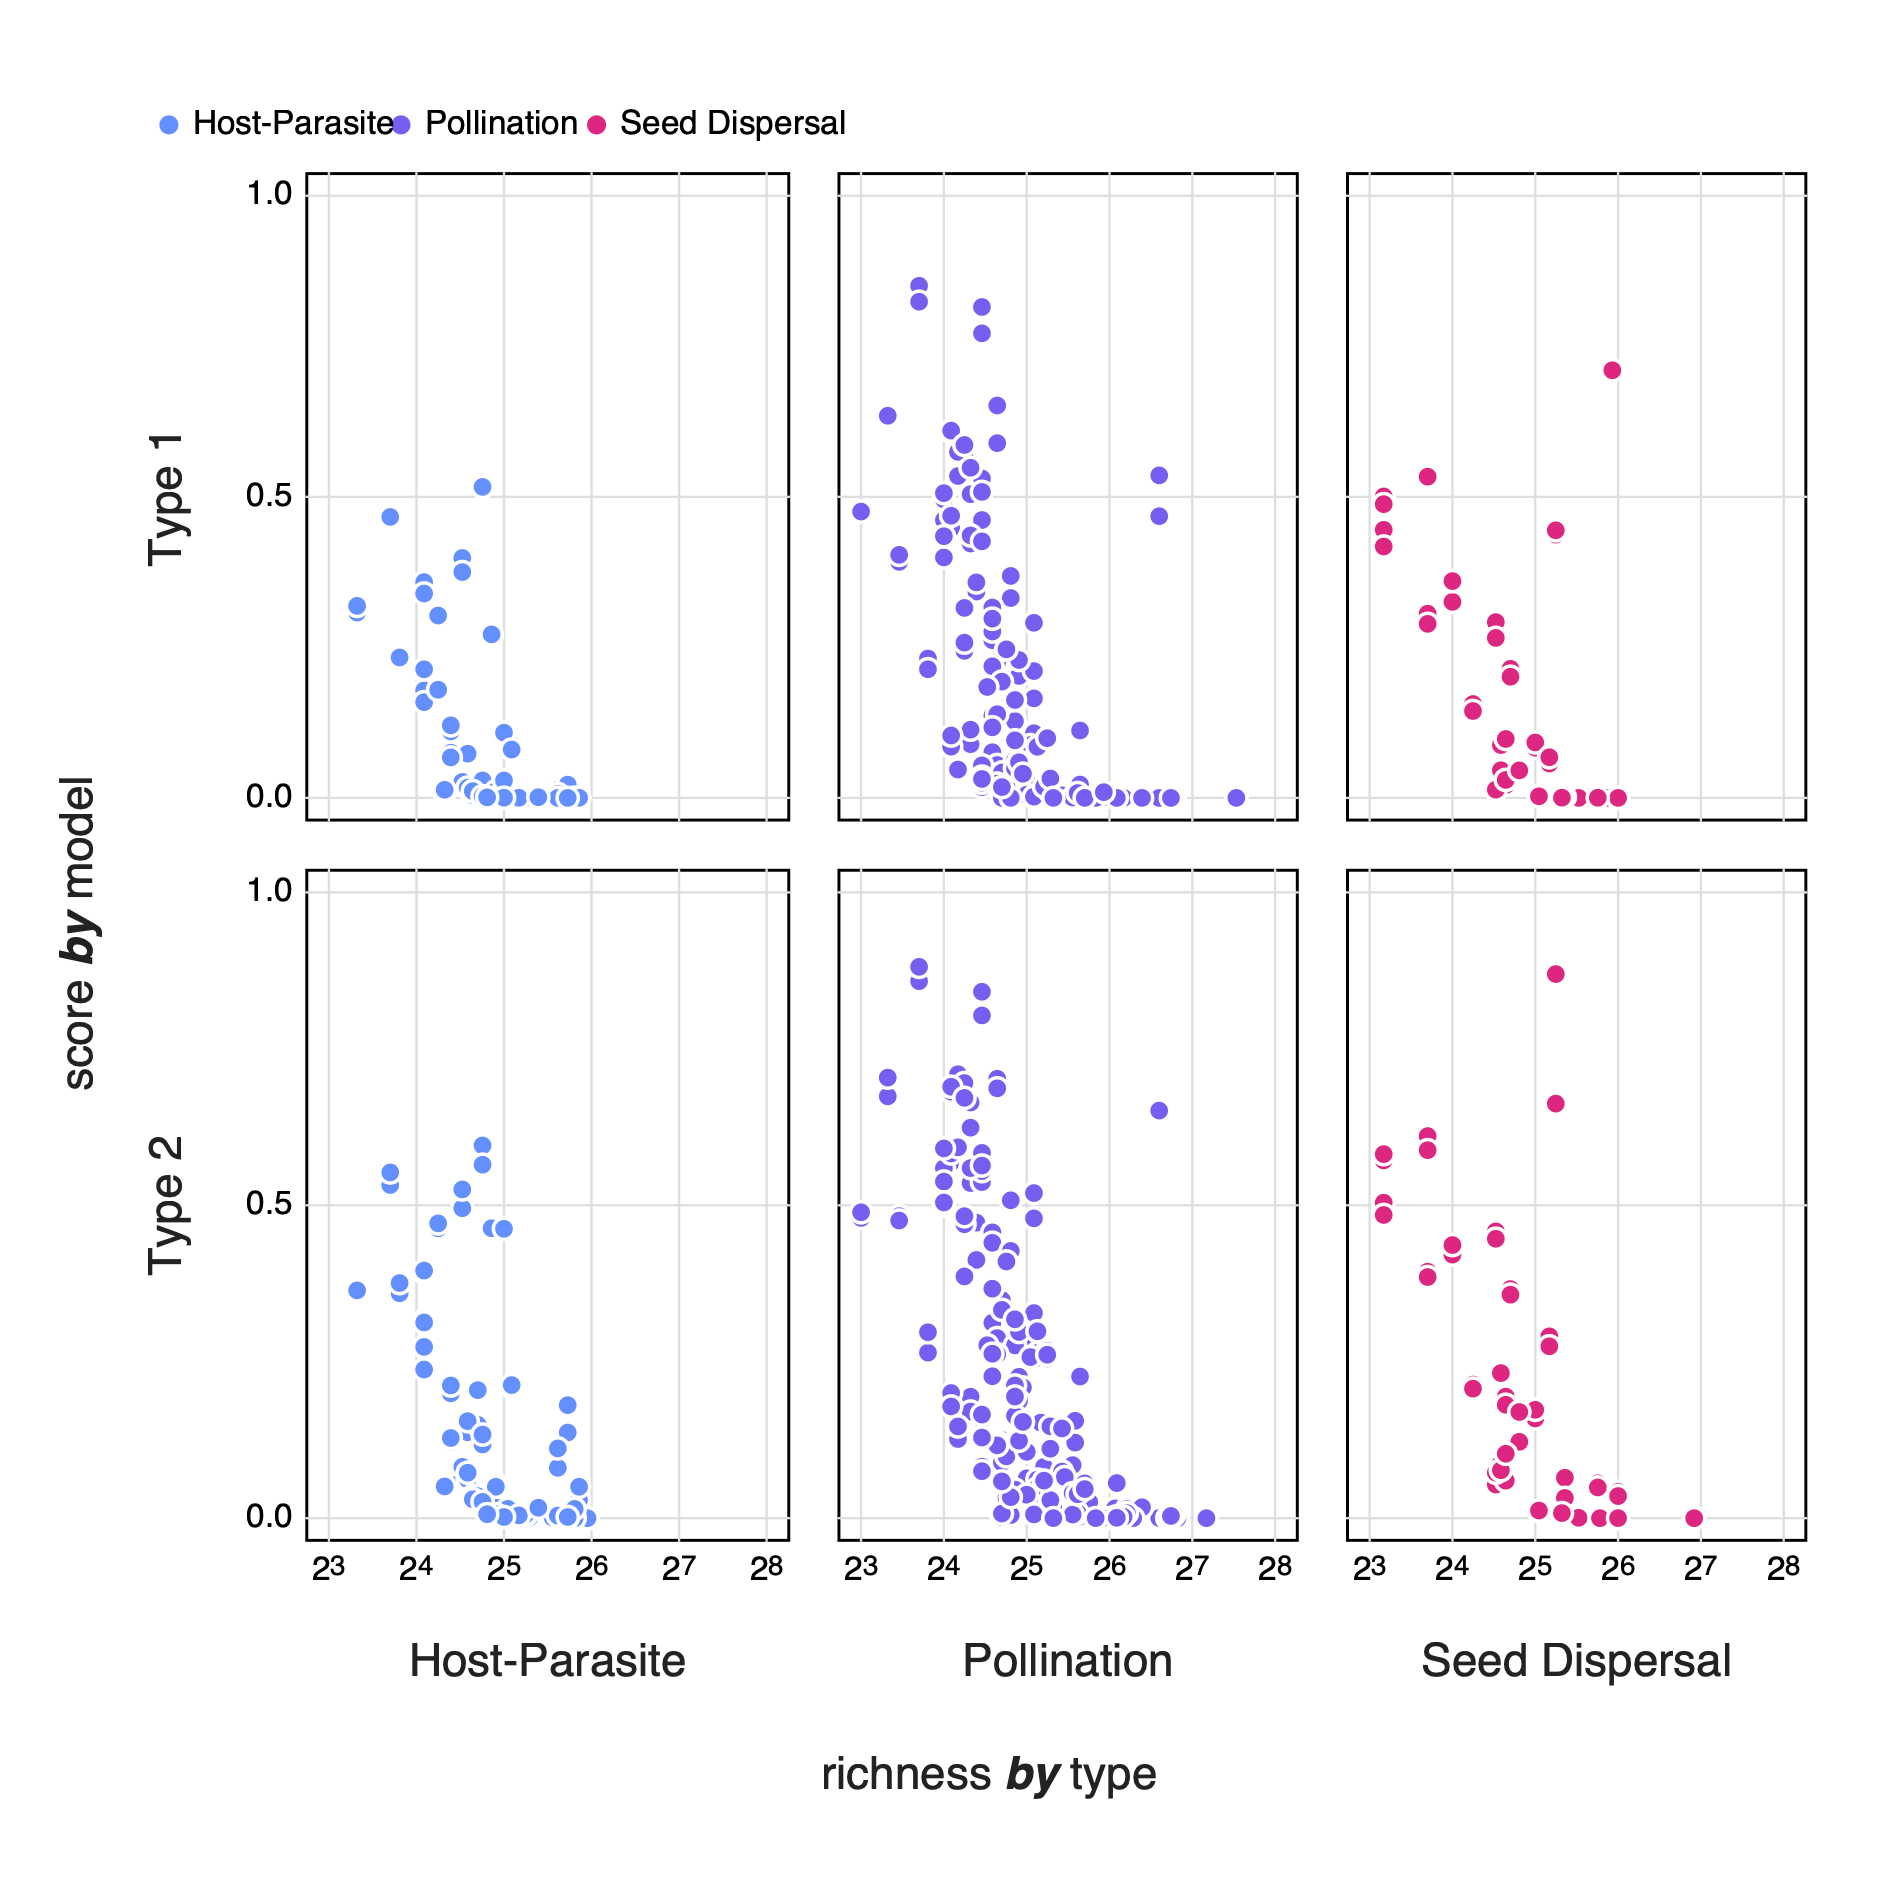
\includegraphics[width=\textwidth]{figures/nullmodel_richness.png}
    \caption{The logistic \(z_i\)-scores of different types of networks for both
Type I and Type II null models compared to the species richness of the network.
Where \(z_i\)-scores below 0.5 indicate networks with an SVD entropy that is
lower \emph{i.e.,} less complex than expected}
    \label{fig:larger}
\end{figure}

\clearpage

\section{Conclusion}\label{conclusion-svd}

We present SVD entropy as a starting point to unifying (and standardising) how
we should approach defining the complexity of ecological networks. The use of a
unified definition will allow us to revisit how complexity relates to the
ecological properties of networks using a standardised method. One important
result from using SVD entropy is that the complexity of ecological networks is
indeed \emph{immense}, yet despite this high complexity networks are still not
reaching their \emph{maximum} potential complexity. We suggest that the assembly
dynamics of networks may explain this observation but this still raises the
question as to why larger (or more mature) networks are not `maintaining' their
expected complexity and prompts further exploration as to the role of ecological
assembly in structuring networks.

\printbibliography{}
\end{refsection}

\endinput
%%
%% End of file `article1.tex'.

%%
%% This is file `article1.tex', % generated with the docstrip utility.
%%
%% The original source files were:
%%
%% dms.dtx  (with options: `article') % Example TeX file for the documentation %
%of the jurabib package % Copyright (C) 1999, 2000, 2001 Jens Berger % See
%dms.ins  for the copyright details.
%% 
%%% ====================================================================
%%%  @LaTeX-file{ %%     filename        = "dms.dtx", %%     author    =
%"Nicolas Beauchemin, Damien Rioux-Lavoie, Victor Fardel, Jonathan Godin", %%
%copyright = "Copyright (C) 2000 , DMS %%                  all rights reserved.
%Copying of this file is %%                  authorized only if either: %%
%(1) you make absolutely no changes to your copy, %%                  including
%name; OR %%                  (2) if you do make changes, you first rename it %%
%to some other name.", %%     address   = "Département de Mathématiques et de
%Statistique", %%     telephone = "514-343-6705", %%     FAX       =
%"514-343-5700", %%     email     = "aide@dms.umontreal.ca (Internet)", %%
%keywords  = "latex, amslatex, ams-latex, theorem", %%     abstract  = " Ce
%fichier est un package conçu pour être %%                  utilisé avec la
%version de LaTeX2e 1995/06/01. Il %%                  est prévue pour la classe
%``amsbook''. Il en %%                  modifie le format des pages, l'entête
%des %%                  sections, etc, afin d'être  conforme au modèle de %%
%mémoire de maîtrise de l'Université de %%                  Montréal. Finalement
%ce fichier est grandement %%                  inspiré du fichier
%amsclass.dtx.", %%     docstring = "The checksum field contains: CRC-16
%checksum, %%                  word count, line count, and character count, as
%%%                  produced by Robert Solovay's checksum utility."}
%%%  ====================================================================


%% To change chapter header dynamically from french to english, use
%%\entetedynamique
\setcounter{corA}{0} % Pour recommancer à compter les def,
                     % theo, etc. à partir de 1
 % Pour écrire un article en français
%% \francais
 % Pour écrire un article en anglais
\anglais
%% NOTE: La plupart des macros ont un nom en anglais. % P.ex. \adresse et
%\address fonctionnent et sont équivalents. % \revue=\journal % \auteur=\author
%% \titre=\title

\doublespacing

%% Les contributions apparaîtront habituellement après % \maketitle (voir un peu
%plus bas). Selon les goûts, il est % possible de mettre les contributions %
%avant la page titre de l'article, simplement en les écrivant % directement ici.
%Par exemple :
 % \cleardoublepage \pdfbookmark[chapter]{Contributions}{contrib1} % Remplacer
 % par contrib2 pour l'article 2 etc. {\bfseries\Large\noindent Contributions de
 % <mon nom> et rôle joué par les coauteurs} J'ai contribué en...
 %
 % Le rôle des coauteurs a été de...

%% Nom de la revue de publication
\revue{Ecography and can be found at https://doi.org/10.1111/ecog.06609}
\article{SpatialBoundaries.jl: Edge detection using spatial wombling}\label{SpatialBoundaries}
%% On peut se référer aux numéros de chapitre ou d'article comme suit. % Si on
%fait % \label{chap:article1}, % alors \ref{chap:article1} donnera le numéro du
%chapitre. On peut ensuite faire % \labelart{art:article1} % et alors
%\ref{art:article1} donnera le numéro d'article. % Par exemple, si cette article
%est le premier article et le deuxième chapitre, % alors si on écrit % Voir le
%chapitre~\ref{chap:article1} (l'article~\ref{art:article1}). % deviendra % Voir
%le chapitre 2 (l'article 1). % Si on veut écrire « premier article » au lieu «
%article 1 », on peut % simplement faire % \ordinal{\ref{art:article1}}~article
%% devient première article % ou % \Ordinal{\ref{art:article1}}~article  %
%devient Première article (avec la majuscule) % Si on est en mode \anglais,
%\ordinal écrire first, second,...

%%%%%%%%%%%%%%%%%%%%%%%%%%%%%%%%%%%%%%%%%%%%%%%%%%%%%%%%%%%%%%%
%%%%%%%%%%%%%%%%%     Contribution     %%%%%%%%%%%%%%%%%%%%%%%% %%%%%%%%%%%%%%%%
%(lire attentivement) %%%%%%%%%%%%%%%%%%%%%%%%
%%%%%%%%%%%%%%%%%%%%%%%%%%%%%%%%%%%%%%%%%%%%%%%%%%%%%%%%%%%%%%%
 % Contribution(s) peronnelle(s) à l'article et rôle joué par tous les
 % coauteur·e·s
 %
 % Nécessaire seulement lorsque vous n'êtes pas seul·e auteur·e. Les
 % contributions peuvent apparaître ailleur dans la thèse. Si \contributions est
 % laissé vide (p.ex. si vous effacez celui ci-bas), aucune contributions ne
 % seront générées sur la page titre de l'article. Vous pouvez alors mettre un
 % \newpage si vous souhaitez que les résumé et abstract soient sur la page
 % suivante.
 %
 % REMARQUE : À peu près toutes les constructions \LaTeX\ sont permises dans les
 % contributions.
 %
 % La commande admet une option [<entête>]
\contributions%[Mes contributions et le rôle des coauteurs]
{ TP and TS designed the study and developed the software. TS was the lead on writing and editing.\\[1cm]
}

%%% INFORMATIONS POUR LA PAGE TITRE
 % Premier auteur·e et adresse

\auteur{Tanya Strydom}
\adresse{Département de Sciences Biologiques, Université de Montréal, Montreal, QC, Canada\\ Québec Centre for Biodiversity Sciences, Montreal, QC, Canada}
\auteur{Timothée Poisot}
\adresse{Département de Sciences Biologiques, Université de Montréal, Montreal, QC, Canada\\ Québec Centre for Biodiversity Sciences, Montreal, QC, Canada}
%

\maketitle
\begin{refsection}

\begin{resume}{wombling spatial, détection des contours, limites, écologie spatiale, logiciel, Julia} Le wombling spatial est une approche permettant de détecter les contours d’un paysage bidimensionnel défini. Ceci est réalisé en calculant le taux et la direction du changement grâce à l’interpolation de points. Cela donne non seulement une approximation de la forme du paysage, mais peut également être utilisé pour identifier des cellules de limites potentielles qui délimitent un passage d'un état à un autre au sein du paysage. Nous présentons ici le package SpatialBoundaries.jl pour Julia, qui a été développé pour implémenter l'algorithme de wombling pour les ensembles de données référencés spatialement pour des paysages échantillonnés de manière uniforme ou aléatoire. D'un point de vue pratique, la fonctionnalité de wombling permet à l'utilisateur de répondre à deux questions: dans quelle mesure et dans quelle direction la variable d’intérêt change-t-elle ? et la fonctionnalité de limites identifie des cellules limites candidates. Nous concluons en fournissant un exemple fonctionnel du package utilisant les différentes couches de plantes ligneuses pour la Grande-Bretagne et l'Irlande à partir de la base de données EarthEnv.
\end{resume}

\begin{abstract}{spatial wombling, edge detection, boundaries, spatial ecology, software, Julia} Spatial wombling is an approach for detecting edges within a defined two-dimensional landscape. This is achieved by calculating the rate and direction of change through the interpolation of points. This not only gives an approximation as to the shape of the landscape but can also be used to identify candidate boundaries cells that delimit a shift from one state to another within the landscape. Here we introduce the SpatialBoundaries.jl package for Julia, which has been developed to implement the wombling algorithm for datasets that are spatially referenced for both uniformly or randomly sampled landscapes.From a practical perspective, the wombling functionality allow the user to answer two questions: how much and in which direction does the variable of interest change? and the boundaries functionality identifies candidate boundary cells. We conclude by providing a working example of the package using the various woody plant layers for Britain and Ireland from the EarthEnv database.
\end{abstract}

\section{Background}\label{background}

There is value in being able to identify boundaries within a landscape
as it provides us with a starting point from which to understand changes
in species assemblages, ecological communities, or even simply to
delineate areas (based on a shared property) into discrete units, for
example ecosystemic regions (\cite{Post2007ProBou, Fortin2000IssRel}).
Here we present a \texttt{Julia} (\cite{Bezanson2017Julia}) package aimed
at detecting boundaries across a specified geographical area by
identifying zones of rapid change using the wombling edge detection
algorithm. This approach was originally developed by \cite{Womble1951DifSys}
in the context of understanding trait variation within a geographic area
and was later modified by \cite{Barbujani1989DetReg} for the purpose of
understanding changes in gene frequencies, although it also has a more
general ecological application with regards to spatial data
(\cite{Fortin2005SpaAna}), serving as a complimentary approach to cluster
analysis (\cite{Fortin1995DelEco}). Wombling has applicability to a wide
range scenarios \emph{e.g.,} trait measurements or genotypes
(\cite{Barbujani1989DetReg}), species interaction networks
(\cite{Fortin2021Network}), and has explicitly been used (to list a few
examples) to detect transitions within a landscape
(\cite{Philibert2008SpaStr, Camarero2000BouDet}), and analyse the spread
of invasive species (\cite{Fitzpatrick2010EcoBou}). Although the origins
of wombling may be rooted in anthropology and has been extensively used
in ecology the potential applicability also extends to other systems
such as high-energy experiments in physics (\cite{Matchev2020FinWom}), or
to understand the genetic-linguistic patterns of European populations
(\cite{Sokal1990GenLan}).

Broadly speaking spatial wombling is an edge-detection algorithm which
traverses a geographic area (for the purpose of this discussion let's
imagine a spatially referenced dataset pertaining to species richness
for each location) and defines this area in terms of the rate ($m$)
and corresponding direction of change ($\theta$) through interpolating
between nearest neighbours. Although the wombling algorithm (as
implemented here) is designed to work with two-dimensional \emph{i.e.,}
planar data (as delimited by $x$ and $y$ --- which would be the
co-ordinates of where species richness was sampled), it is beneficial to
view this plane as a three-dimensional object (or series of curves), as
shown in \autoref{fig:concept_womble}, panel A. Here the `amplitude' of the curvature of
the plane is determined by the value of $z$ (species richness) and the
rate and direction of change is calculated by using the first-order
partial derivative $\partial$ of the surface (curve) as described by
$f(x,y)$. This then gives us an indication of how steep the
gradient/curve ($m$) is between neighbouring cells as well as the
direction (from the `low' to the `high' point; $\theta$) of the slope
(panel B, \autoref{fig:concept_womble}). Large values of $m$ are associated with zones
of rapid change in the landscape and are indicative of a shift from one
`state' to another \emph{i.e.,} a potential ecological boundary within
the landscape (\cite{Fortin2005SpaAna}; dashed line in panel C,
\autoref{fig:concept_womble}). One benefit of the wombling approach is that
interpolation is not necessarily restricted to a rectangular
($2 \times 2$) window (that would entail a landscape where points are
regularly arranged in space) and can easily be re-written so as to
accommodate points that are not regularly arranged across space (as per
\cite{Fortin1994EdgDet}), thereby giving the user more flexibility with
regards to how the sampling points are arranged (\emph{i.e.,} sampled)
across the landscape.

\begin{figure}[h]
    \centering
    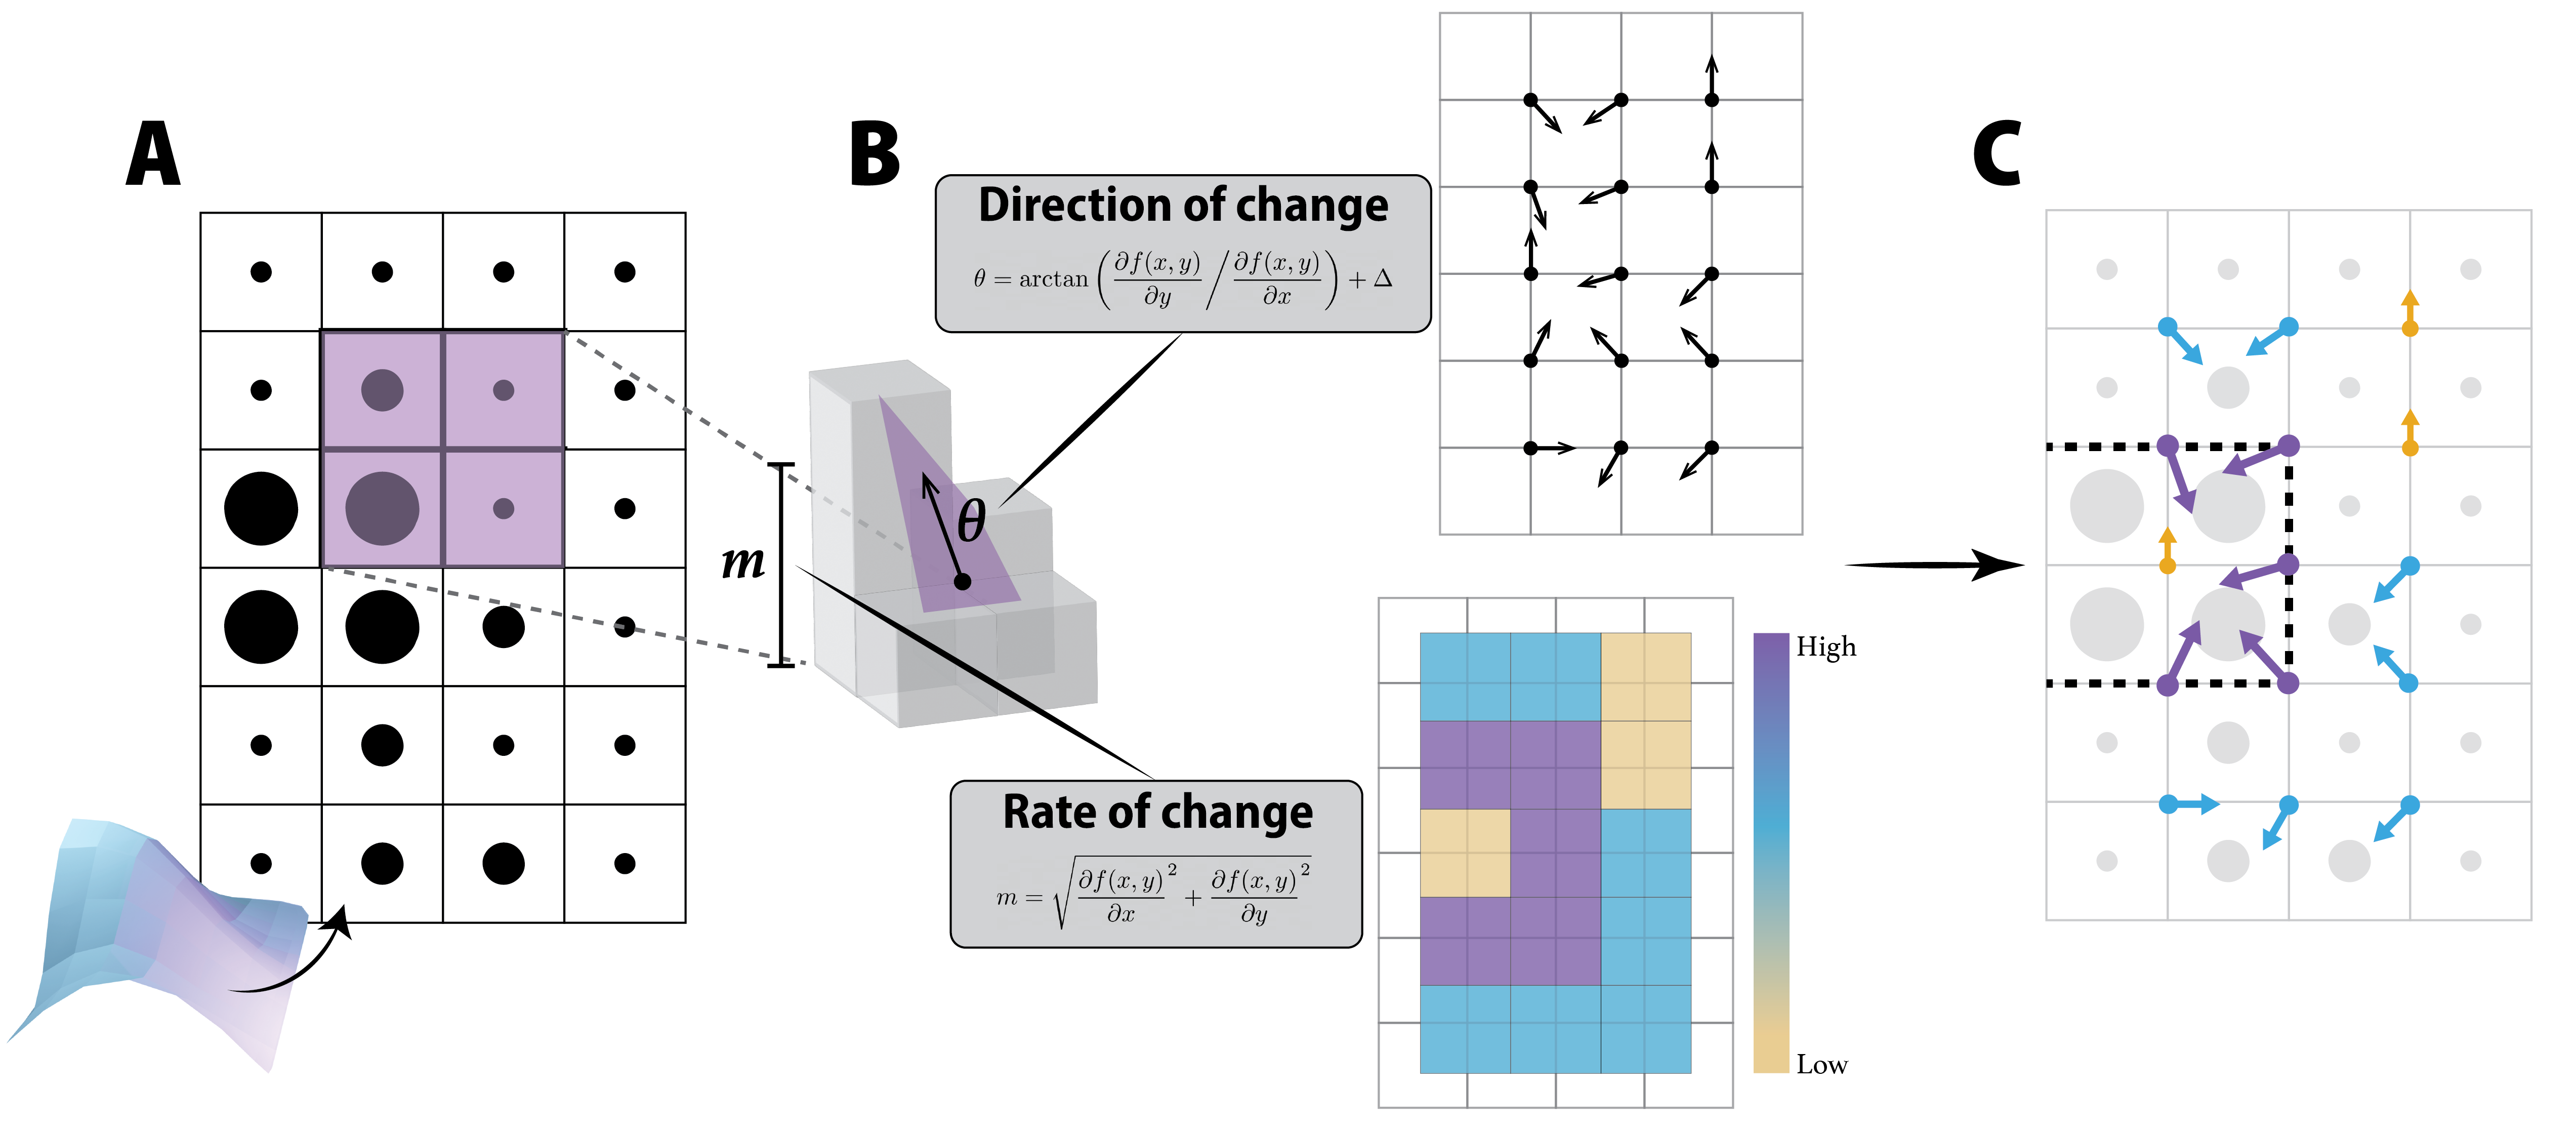
\includegraphics[width=\textwidth]{figures/fig_concept.png}
    \caption{A visual conceptualisation of how the wombling algorithm
interpolates points across a geographical area (in this case the points
are regularly arrange in space) for a variable of interest (\(z\)) to
calculate the rate ($m$) as well as the direction ($\theta$) of
change. Here the sampled landscape is shown in panel A with the size of
the points correlating to the magnitude if the variable of interest
($z$). Panel B shows the two components of the landscape once wombled,
which are then combined and superimposed across the original landscape
in panel C, with the dashed line indicating a candidate boundary. Here
the colours as well as the size of the arrows indicate the rate of
change and the direction should be interpreted as moving from the `low'
to the `high' point. Note that the dimensions of the wombled landscapes
(B) will be smaller than the original landscape (A) due to the
interpolation process \emph{i.e.,} where we originally had an
\(n \times r\) grid we now have an (\(n\) - 1)(\(r\) - 1) sized
grid.}
    \label{fig:concept_womble}
\end{figure}

\subsection{Rate of change}\label{rate-of-change}

The rate of change ($m$) can be used to find the zones of rapid change
within the geographical area --- which, in turn, can be used to identify
potential candidate boundaries. The rate of change is calculated as
follows:

\begin{equation} \label{eq:1}
m = \sqrt{\frac{\partial f(x,y)}{\partial x}^2 + \frac{\partial f(x,y)}{\partial y}^2}
\end{equation}

Where \(f(x,y)\) can be expanded as:

$$f(x,y) = z_{1}(1-x)(1-y) + z_{2}x(1-y) + z_{3}x y + z_{4}(1-x)y$$

For convenience the values of the centroid of the `search window'
\emph{i.e.,} \(x\) and \(y\) can be standardised to 0.5 when working with
points regularly arranged in space. Additionally, as we are
interpolating between points, it should also be noted that the original
\(n*r\) geographical area will now be an \((n -1)(r - 1)\) sized grid
(\emph{i.e.,} one less row and one less column of values for the wombled
landscape as illustrated in panel C of \autoref{fig:concept_womble}).

When we are working with points that are irregularly arranged within the
geographical area it is possible to use triangulation wombling
(\cite{Fortin2005SpaAna, Fortin2021Network, Fortin1994EdgDet}). Here the
approach to wombling has been modified by \cite{Fortin1992DetEco} so as to
interpolate the plane between the three nearest neighbours (as opposed
to the usual \(2 \times 2\) grid). Nearest neighbours are found by using
the Delaunay triangulation algorithm (\cite{Delaunay1934SphVid}) after
which the rate of change is still calculated in the same manner as in
\autoref{eq:1}, however as we are now only working with a three-point
`window' \(f(x,y)\) will be defined as:

$$f(x,y) = ax + by + c$$

where

$$\left[ \begin{array}{ccc} a & b & c \end{array} \right] = 
\left[ {\begin{array}{ccc}
   x_{1} & y_{1} & 1\\
   x_{2} & y_{2} & 1\\
   x_{3} & y_{3} & 1\\
  \end{array} } \right]^{-1}\cdot
  \left[
  \begin{array}{ccc} z_{1} & z_{2} & z_{3} \end{array} \right]$$

and the \(x\) and \(y\) co-ordinates of the centroid of the triangle
formed by the three points are calculated as follows:

$$ \Big( \frac{x_{1} + x_{2} + x_{3}}{3} \Big), \Big( \frac{y_{1} + y_{2} + y_{3}}{3} \Big) $$

\subsection{Direction of change}\label{direction-of-change}

It is also possible to calculate a corresponding direction (\(\theta\))
for each rate of change (noting that the same equation can be used for
both lattice and triangulation wombling). This is calculated as:

$$\theta = \arctan \left( \frac{\partial f(x,y)}{\partial y} \bigg/ \frac{\partial f(x,y)}{\partial x} \right) + \Delta$$

$$\text{where} \quad \Delta =
\left\{ \begin{array}{ccc}
    0 \degree & \text{if} & \frac{\partial f(x,y)}{\partial x} \geq 0 \\
    180 \degree & \text{if} & \frac{\partial f(x,y)}{\partial x} < 0 \\
\end{array} \right\}$$

This gives the direction of change which, as the name implies, indicates
the direction the rate of change is `travelling'. The direction of
change should be interpreted as wind direction \emph{i.e.,} where the
change is coming from and not where it is moving towards. As is the
nature of maths when the rate of change is zero it is still possible to
calculate a \emph{real} direction for the non-change --- which will be
180$^{\circ}$. This means it is possible to think of and use the
direction of change independently of calculating boundaries \emph{per
se} and can be used to inform how the landscape is behaving/changing in
a more `continuous' way as opposed to discrete zones/boundaries. For
example if changes in species richness are more gradual (rate of change
is near constant) but the the direction of change is consistently East
to West (\emph{i.e.,} 90$^{\circ}$) we can still infer that species
richness is more or less uniformly increasing in a South-North direction
(this is somewhat exemplified in the direction of change landscape of
panel B in \autoref{fig:concept_womble} where the dominant direction of change is
East-West).

\subsection{Candidate boundaries}\label{candidate-boundaries}

Detecting boundaries \emph{i.e.,} areas where the angle of the landscape
transitions sharply is surprisingly simple. After having calculated the
rate of change (\(m\)) for the geographical area it is possible to use
these values to identify and assign potential boundaries
(\cite{Fortin2005SpaAna, Oden1993CatWom, Fortin1995DelEco}). As large
rate of change values are indicative of a steep gradient it stands to
reason that these points are indicative of a shift from one state to
another \emph{i.e.,} indicative of a boundary. Following the approach
outlined in \cite{Fortin2005SpaAna} a threshold value (or percentile class)
can be set and will determine what proportion of cells will be retained
as potential boundaries. For example if using a 0.1 threshold then the
highest 10\% of points (which are ranked based on \(m\)) will be
classified as candidate boundaries. Note that points with the same rate
of change will be assigned the same rank meaning that more than 10\% of
the \((n -1)(r - 1)\) could potentially be identified as candidate
boundary cells. This approach to identifying potential boundary cells is
not the sole approach and there are other ways and nuances from which to
approach boundary estimation, such as the use of Voronoi tessellations
(\cite{Fortin1995DelEco, Oden1993CatWom, Matchev2020FinWom}).

\section{Methods and features}\label{methods-and-features}

\texttt{SpatialBoundaries} v0.0.3 implements the Wombling algorithm
within the \texttt{Julia} ecosystem and is made available under the
permissive MIT license. The source code (along with more extensive
documentation) can be found at
\url{https://poisotlab.github.io/SpatialBoundaries.jl/}. This is an open
project and is thus open to contributions. The package itself has two
main functions 1) calculate the rate (\(m\)) and direction (\(\theta\))
of change for landscapes for points that are both regularly (\emph{i.e.,}
lattice wombling) and irregularly arranged cross space (triangulation
wombling) arranged in space using the \texttt{wombling} function (for
which layers can also be aggregated using \texttt{mean}), and 2)
identifying candidate boundary cells based on a user defined threshold
value using the \texttt{boundaries} function. Objects that have been
passed through a wombling function are of the \texttt{Womble} abstract
type (which has the two sub-types of \texttt{LatticeWomble} and
\texttt{TriangulationWomble}). This package is, to the best of our
knowledge, the only package to implement the Wombling algorithm within
\texttt{Julia}.

\subsection{Wombling}\label{wombling}

The \texttt{wombling} function calculates and outputs both the rate
(\(m\)) and direction (\(\theta\); where the direction is denoted from
the `low' to the `high' point) of change for a given geographical area.
Leveraging the multiple dispatch within \texttt{Julia} this one function
will execute either the lattice or triangulation wombling algorithm
depending on the structure (spatial referencing) of the input dataset,
meaning that it does not need to be user specified. When a \emph{matrix}
of \(z\) values is used (where the row and column id's act as the
co-ordinates) the lattice wombling algorithm will be executed and when
three \emph{vectors} (consisting of the co-ordinates (\(x\) and \(y\)),
and \(z\) values respectively) the triangulation wombling algorithm is
executed. The resulting output object will have two components (\(m\)
and \(\theta\)) and will be typed based on the wombling method used.
That is a uniform matrix will result in an object of the type
\texttt{LatticeWomble} and irregularly arranged points will be of the
type \texttt{TriangulationWomble}.

\subsection{Overall mean wombling
value}\label{overall-mean-wombling-value}

The \texttt{mean} function calculates the Overall mean wombling value.
The methodology stems from the Overall Mean Lattice-Wombling Value
(\(\bar{m}\)) used by \cite{Fortin1994EdgDet} in which multiple surfaces
(think different \(z\) variables) can be overlaid for the purpose of
finding the mean rates and directions of change for a composite
landscape. The mean rate of change can be defined as the average of
\(m\) values (for a specific centroid) for the given set of surfaces and
the same is done for the direction of change using the \(\theta\)
values. Alongside the mean the standard deviation is also calculated for
both the rate and direction of change. Although \cite{Fortin1994EdgDet} only
present this approach for lattice wombled landscapes we have extended
the functionality to include both lattice and triangulation wombled
types. This is provided that the landscape (\emph{i.e.,} co-ordinates) of
the different surfaces are \emph{exactly} the same. Note here that the
original wombling type is retained and the output data will remain
either type \texttt{LatticeWomble} or \texttt{TriangulationWomble}.

\subsection{Boundaries}\label{boundaries}

The \texttt{boundaries} function takes the rate of change (\(m\)) of an
object of either of the two \texttt{Womble} types (\emph{i.e.,}
\texttt{LatticeWomble} or \texttt{TriangulationWomble}), and identifies
potential boundary cells based on a user specified threshold (with the
default being 0.1). As opposed to selecting only one threshold value we
recommend inputting a range of threshold values into the
\texttt{boundaries} function to assess how it changes the number of
points retained (\emph{i.e.,} boundary cells identified). For example we
might see sharp transitions in the number of points that are retained as
the threshold value is increased. This inflection point is probably the
ideal threshold value to use for boundary selection as a rapid increase
in the number of points retained is indicative of a large number of
cells with the same rate of change.

\section{Woody areas of the Hawaiian Islands: a wombling
example}\label{woody-areas-of-the-hawaiian-islands-a-wombling-example}

Below is an example using the various functions within
\texttt{SpatialBoundaries} to estimate boundaries for (\emph{i.e.,}
patches of) wooded areas on the Southwestern islands of the Hawaiian
Islands using landcover data from the EarthEnv project
(\cite{Tuanmu2014Glo1km}) as well as integrating some functionality from
\texttt{SimpleSDMLayers} (\cite{Dansereau2021Simplesdmlayers}) for easier work with the spatial nature of the input data. The \texttt{SpatialBoundaries}
package works really well with \texttt{SimpleSDMLayers}, so that you can
(i) apply wombling and boundaries finding to a \texttt{SimpleSDMLayer}
object, and (ii) convert the output of a \texttt{Womble} object to a
\emph{pair} of \texttt{SimpleSDMLayer} corresponding to the rate and
direction of change.

Because there are four different layers in the EarthEnv database that
represent different types of woody cover we will use the overall mean
wombling value. As the data are arranged in a matrix \emph{i.e.,} a
lattice this example will focus on lattice wombling, however for
triangulation wombling the implementation of functions and workflow
would look similar with the exception that the input data would be
structured differently (as three vectors of \(x\), \(y\), \(z\)) and the
output data would be typed as \texttt{TriangulationWomble} objects.

\begin{verbatim}
using SpatialBoundaries
using SpeciesDistributionToolkit
using CairoMakie
import Plots
\end{verbatim}

Note that the warning about dependencies is a side-effect of loading
some functionalities for \texttt{SimpleSDMLayers} as part of
\texttt{SpatialBoundaries}, and can safely be ignored.

First we can start by defining the extent of the Southwestern islands of
Hawaii, which can be used to restrict the extraction of the various
landcover layers from the EarthEnv database. We do the actual database
querying using \texttt{SimpleSDMLayers}.

\begin{verbatim}
hawaii = (left = -160.2, right = -154.5, bottom = 18.6, top = 22.5)
dataprovider = RasterData(EarthEnv, LandCover)
landcover_classes = SimpleSDMDatasets.layers(dataprovider)
landcover = [SimpleSDMPredictor(dataprovider; 
                layer=class, full=true, hawaii...) 
                for class in landcover_classes]
\end{verbatim}

We can remove all the areas that contain 100\% water from the landcover
data as our question of interest is restricted to the terrestrial realm.
We do this by using the ``Open Water'' layer to mask over each of the
landcover layers individually:

\begin{verbatim}
ow_index = findfirst(isequal("Open Water"), landcover_classes)
not_water = landcover[ow_index] .!== 0x64
lc = [mask(not_water, layer) for layer in landcover]
\end{verbatim}

As layers one through four of the EarthEnv data are concerned with data
on woody cover (\emph{i.e.,} ``Evergreen/Deciduous Needleleaf Trees'',
``Evergreen Broadleaf Trees'', ``Deciduous Broadleaf Trees'', and
``Mixed/Other Trees'') we will work with only these layers. To get a
sense of the overall structure of raw landcover components we can sum
these four layers and plot the total woody cover for the Southwestern
islands (The code for the plot below will give us panel A in
\autoref{fig:example_womble}).

\begin{verbatim}
classes_with_trees = findall(contains.(landcover_classes, "Trees"))
tree_lc = convert(Float32, reduce(+, lc[classes_with_trees]))
heatmap(tree_lc; colormap=:linear_kbgyw_5_98_c62_n256)
\end{verbatim}

\begin{figure}[h]
    \centering
    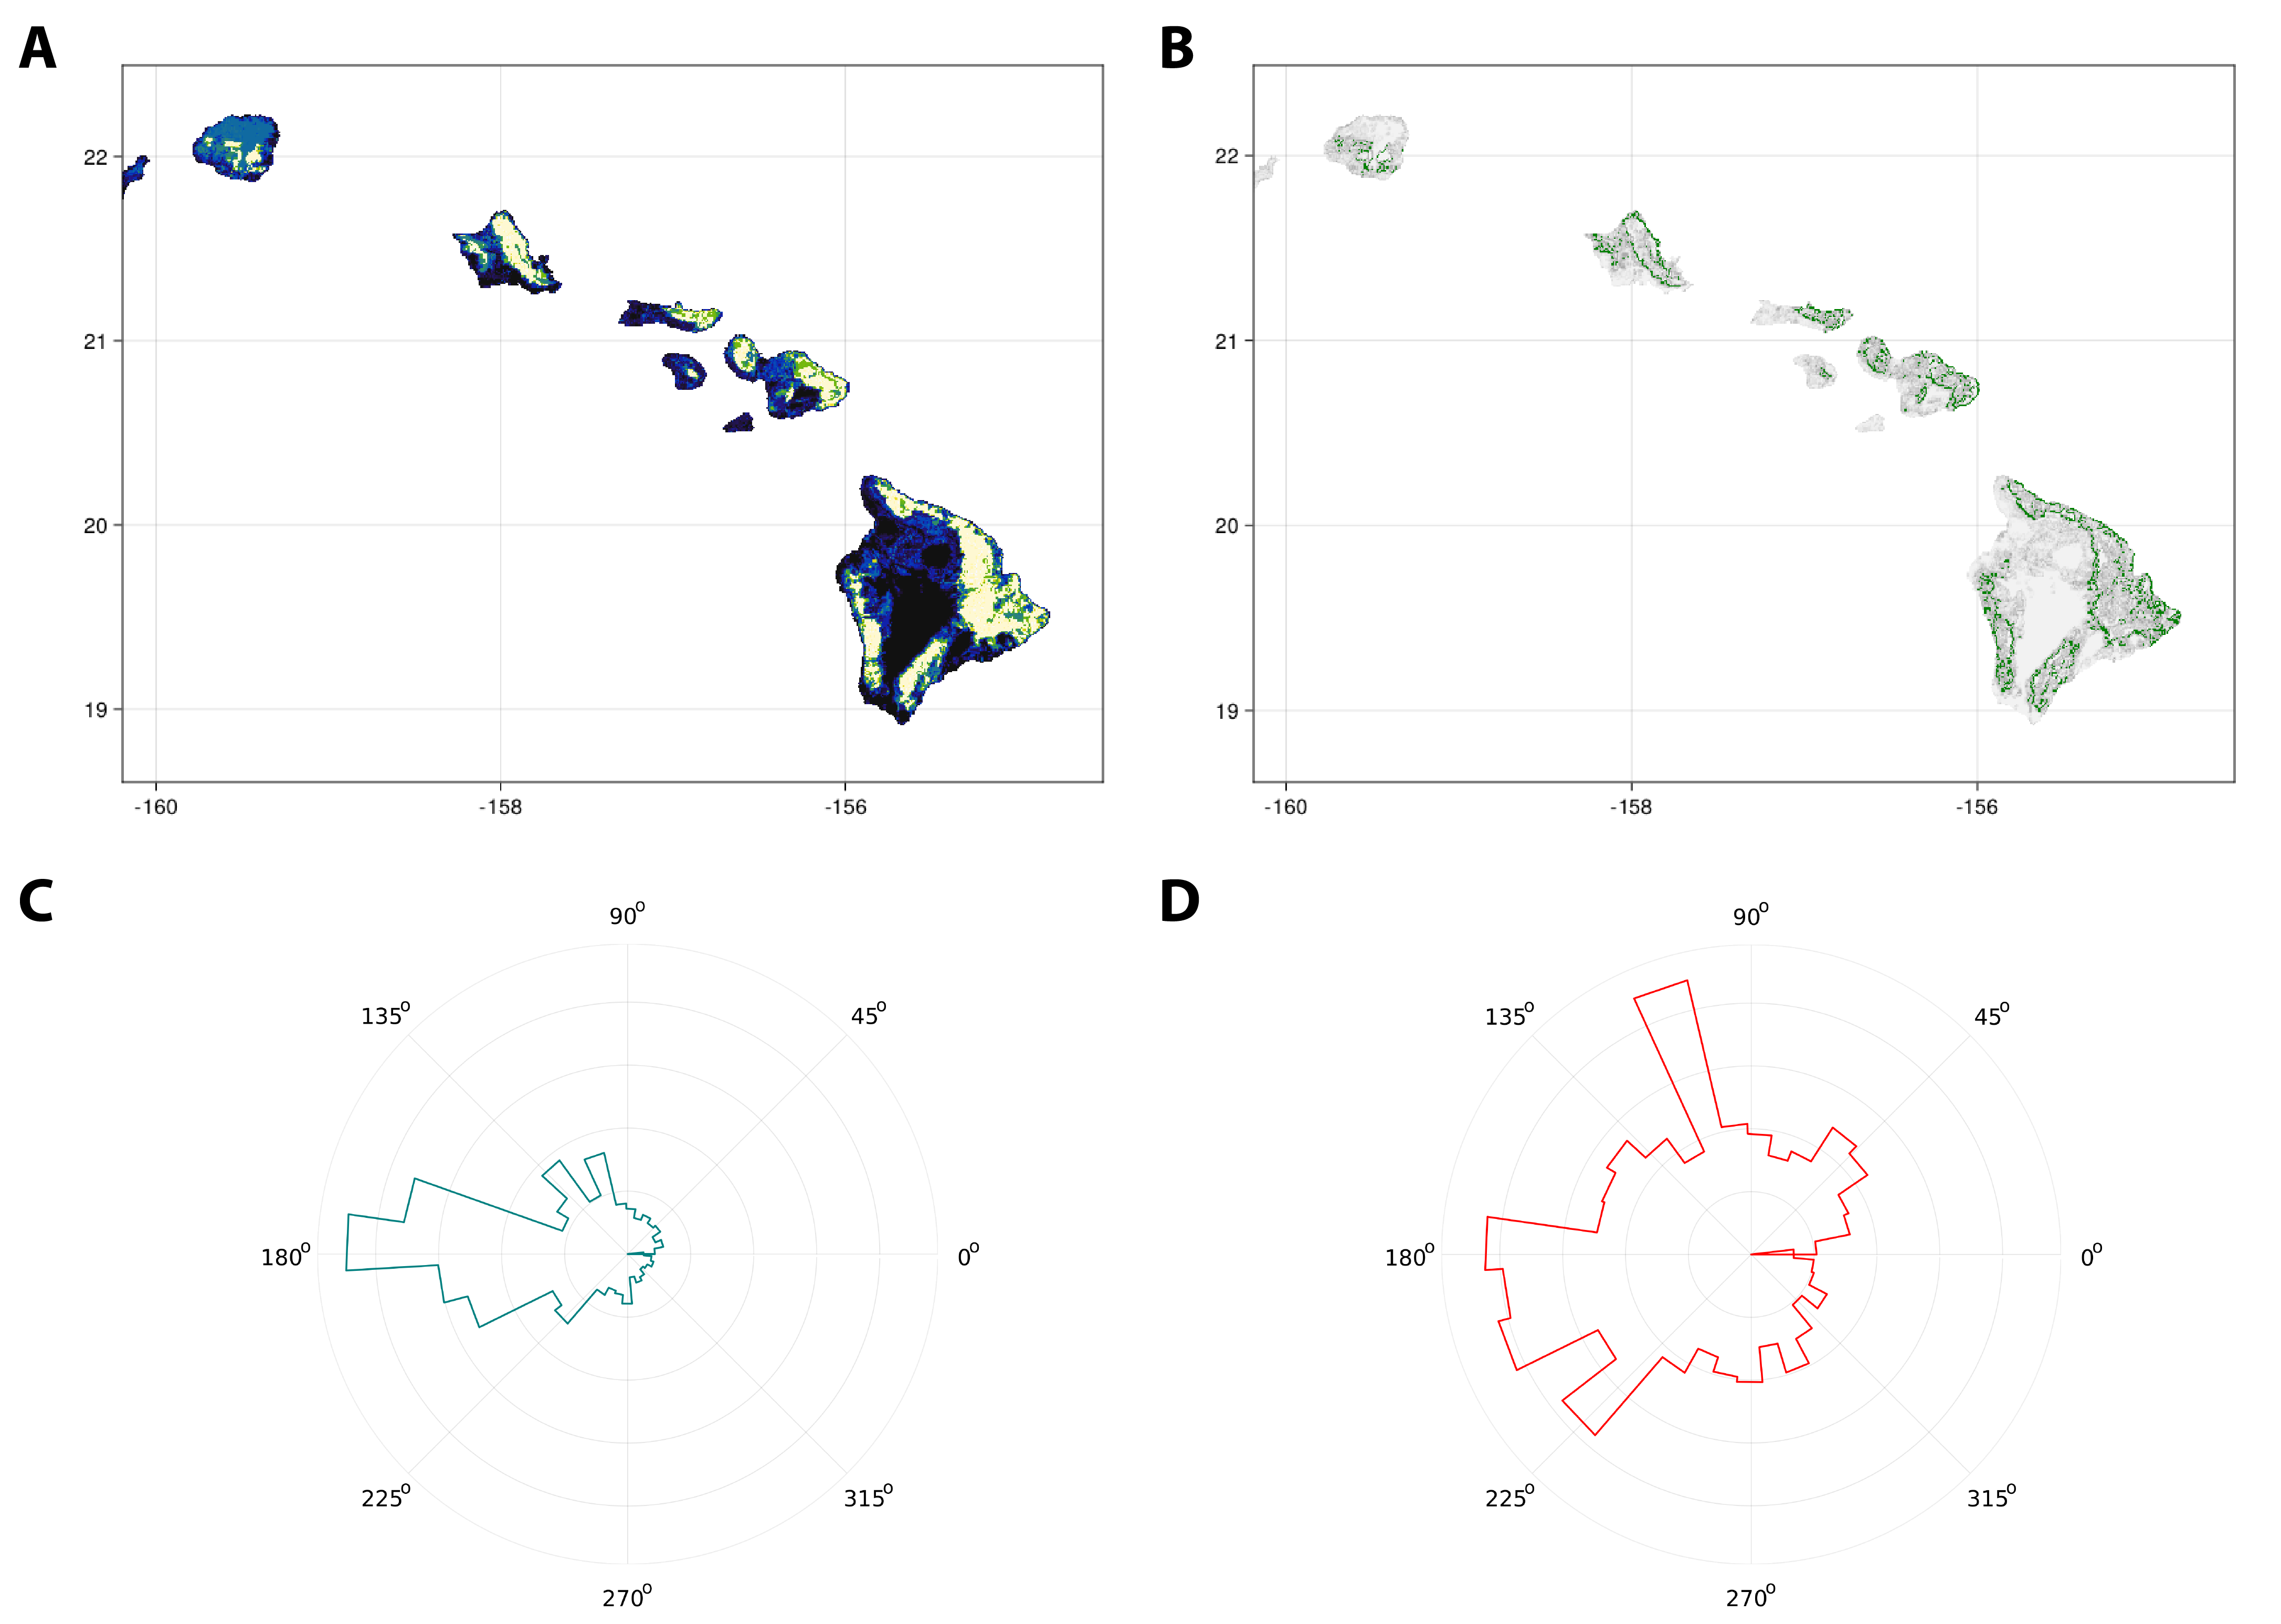
\includegraphics[width=\textwidth]{figures/fig_eg.png}
    \caption{\textbf{A} Woody plant coverage for Southwestern islands of the
Hawaiian Islands based on the sum of the cover for layers 1-4 from the
EarthEnv project. \textbf{B} the overall mean rate of change
(\emph{i.e.,} the composite of the wombled layers for layers 1-4) but
only for the cells identified as candidate boundary cells when using a
10\% threshold, with identified boundaries (shown in green) over the
rate of change (shown in levels of grey). The final two panels show the
direction of change for all cells (\textbf{C}) and only for cells
considered to be candidate boundary cells
(\textbf{D}).}
    \label{fig:example_womble}
\end{figure}

Although we have previously summed the four landcover layers for the
actual wombling part we will apply the wombling function to each layer
before we calculate the overall mean wombling value. We can broadcast
\texttt{wombling} in an element-wise fashion to the four different woody
cover layers. This will give as a vector containing four
\texttt{LatticeWomble} objects (since the input data was in the form of
a matrix).

\begin{verbatim}
wombled_layers = wombling.(lc[classes_with_trees])
\end{verbatim}

As we are interested in overall woody cover for Southwestern islands we
can take the \texttt{wombled\_layers} vector and use them with the
\texttt{mean} function to get the overall mean wombling value of the
rate and direction of change for woody cover. This will `flatten' the
four wombled layers into a single \texttt{LatticeWomble} object.

\begin{verbatim}
wombled_mean = mean(wombled_layers)
\end{verbatim}

From the \texttt{wombled\_mean} object we can `extract' the layers for
both the mean rate and direction of change. For ease of plotting we will
also convert these layers to \texttt{SimpleSDMPredictor} type objects.
It is also possible to call these matrices directly from the
\texttt{wombled\_mean} object, which has fields for \(m\) (the magnitude
of change) and \(\theta\) (the direction of change).

\begin{verbatim}
rate, direction = SimpleSDMPredictor(wombled_mean)
\end{verbatim}

Lastly we can identify candidate boundaries using the
\texttt{boundaries}. Here we will use a thresholding value (t) of 0.1
and save these candidate boundary cells as \texttt{b}. Note that we are
now working with a \texttt{SimpleSDMResponse} object and this is simply
for ease of plotting.

\begin{verbatim}
b = similar(rate)
b.grid[boundaries(wombled_mean, 0.1; ignorezero = true)] .= 1.0
\end{verbatim}

In addition to being used to help find candidate boundary cells we can
also use this object (\texttt{b}) as masking layer when visualising
wombling outputs. In this case we can view the \texttt{rate} layer in a
similar fashion to the original landcover layer but by masking it with
\texttt{b} we only plot the candidate boundaries (B in \autoref{fig:example_womble})
\emph{i.e.,} the cells with the top 10\% of highest rate of change
values. For visualisation we will overlay the identified boundaries (in
green) over the rate of change (in levels of grey)

\begin{verbatim}
heatmap(rate, colormap=[:grey95, :grey5])
heatmap!(b, colormap=[:transparent, :green])
current_figure()
\end{verbatim}

For this example we will plot the direction of change as radial plots
(third and fourth panels in \autoref{fig:example_womble}) to get an idea of the
prominent direction of change. Here we will plot \emph{all} the
direction values from \texttt{direction} for which the rate of change is
greater than zero (so as to avoid denoting directions for a slope that
does not exist) as well as the \texttt{direction} values from only
candidate cells using the same masking principle as what we did for the
rate of change. It is of course also possible to forgo the radial plots
and plot the direction of change in the same manner as the rate of
change should one wish.

Before we plot let us create our two `masked layers'. For all direction
values for which there is a corresponding rate of change greater than
zero we can use \texttt{rate} as a masking layer but first replace all
zero values with `nothing'. For the candidate boundary cells we can
simply mask \texttt{direction} with \texttt{b} as we did for the rate of
change.

\begin{verbatim}
direction_all = mask(replace(rate, 0 => nothing), direction)

direction_candidate = mask(b, direction)
\end{verbatim}

Because stephist() requires a vector of radians for plotting we must
first collect the cells and convert them from degrees to radians. Then
we can start by plotting the direction of change of \emph{all} cells (C
in \autoref{fig:example_womble}).

\begin{verbatim}
Plots.stephist(
         deg2rad.(values(direction_all));
         proj=:polar,
         lab="",
         c=:teal,
         nbins = 36,
         yshowaxis=false,
         normalize = false,
         dpi=600)
\end{verbatim}

Followed by plotting the direction of change only for cells that are
considered as candidate boundary cells (D in \autoref{fig:example_womble}).

\begin{verbatim}
Plots.stephist(
                deg2rad.(values(direction_candidate));
                proj=:polar,
                lab="",
                c=:red,
                nbins = 36,
                yshowaxis=false,
                normalize = false,
                dpi=600)
\end{verbatim}

\section{Summary}\label{summary}

Edge and boundary detection (as well as their delineation) is an
important and valuable concept in spatial ecology
(\cite{Cadenasso2003FraThe}) of which wombling serves as an approach that
is flexible in its execution (owing to the non-lattice or triangulation
capacity of the function) (\cite{Fortin2005SpaAna, Fortin1994EdgDet}) as
well as it's capacity to detect more nuanced landscape changes as
opposed to being limited to more abrupt discontinuities such as
cliffs/ridges by reducing noise in the landscape
(\cite{Matchev2020FinWom}). Wombling sets us up to answer two questions
about the geographic area of interest: at what rate and in which
direction does the variable of interest change? This of course has value
when it comes to evaluating the variation (or uniformity for that
matter) of a suite of ecological variables as well as how they may vary
with relation to each other.

\texttt{SpatialBoundaries.jl} provides the toolset with which to
implement both lattice and triangulation wombling using the
\texttt{wombling} function - multiple dispatch means that the structure
of the input dataset will determine exactly which algorithm is
implemented. This will simultaneously calculate both the rate and
direction of change and if desired multiple sets of different layers of
the same geographic area but defined by different
\(z\)-variables/surfaces can be aggregated and averaged to calculate the
overall mean wombling value. Both \texttt{wombling} and \texttt{mean}
will return objects of the type \texttt{Womble} of either the sub-type
\texttt{LatticeWomble} or \texttt{TriangulationWomble} depending on
which method was used. An object of any sub-type \texttt{Womble} can be
input into the \texttt{boundaries} function so as to identify cells that
can be considered as candidate boundaries based on a user specified
threshold.

\textbf{Acknowledgements:} We acknowledge that this study was conducted
on land within the traditional unceded territory of the Saint Lawrence
Iroquoian, Anishinabewaki, Mohawk, Huron-Wendat, and Omàmiwininiwak
nations. TS and TP are funded by a donation from the Courtois
Foundation.

\printbibliography{}
\end{refsection}

\endinput
%%
\anglais
\doublespacing
\chapter{General Conclusion}\label{Conclusion}
\begin{refsection}

As species interaction networks are determined by ecological and evolutionary mechanisms that have played out across spatial and temporal scales the measures that define their structure (properties) are also capturing information about the processes that have played a role in structuring them. Thus the properties of a network are not only representative of its structure but also a measure of \emph{how} different processes have played a role in determining it, meaning that when we are measuring the property of a network we are also capturing information about the network. This information is something that can be used for making predictions about network structure, \emph{e.g.,} it has been shown that it is possible to to make network-level inferences with very low-level data \cite{MacDonald2020Revisiting, Banville2023What}, or to help make within network predictions to find missing links (\cite{Poisot2023Network, Stock2021Pairwise}). The ability to use a 'simple' measure of the species community for a given location (such as species richness) and to have an estimate of the structure of the potential network (such as connectance) is truly amazing and speaks to how much information we are able to extract either from species networks, or alternatively use to make network predictions. This is something is echoed throughout this thesis.

\section{What we have learnt}

\subsection{Prediction is attainable and feasible}

Chapter~\ref{Foodweb} showcases that with very little 'real world' information we can make accurate predictions by using the information that is 'encoded' in existing interaction networks. This is also echoed in Chapter~\ref{SVD}, where we can see the \emph{immense} amount of information that networks contain and that it is a case of finding ways to access and use this information and, in this instance, using it to make network predictions. It is also clear that this information can go a long way, the metaweb for Canada shared only 4\% of species with its European counterpart, yet we were able to recover 91\% of the interactions. From an ecological perspective this highlights how the laws governing interactions (\emph{sensu} common backbones from \cite{BramonMora2018Identifying}) are being conserved phylogenetically (\cite{Davies2021EcoRed, Elmasri2020HieBay, Gomez2010EcoInt}). From a more practical perspective we show that this transfer learning framework is primed to be adopted as a 'gap-filling' tool as it does not require \emph{extensive} data or computational resources. It is worth noting that in order to predict the Canadian metaweb one only needs to access three different data sources (the species community for Canada, the European metaweb, and a well resolved phylogeny) and that it is possible to execute the required code on a standard laptop, underscoring the lightweight nature of the framework. Finally, the transfer learning framework itself has a lot of scope to be modified should the transfer task have a different set of \emph{e.g.,} data requirements (this is discussed extensively in \autoref{Perspectives}). 

As highlighted by the broad, scoping, discussion in Chapter~\ref{Roadmap} transfer learning is not the only way to approach transfer learning and there are a variety of methodological approaches and data sources that we can tap into when wanting to make network predictions (\autoref{fig:conceptual}. Having a body of work that explicitly addresses the idea of machine learning for network prediction will be particularly valuable as the popularity and interest in alternative 'non-statistical' methods continues to grow within the field of ecology and evolution (\cite{Pichler2023Machine, Cuff2023Chapter}). This chapter also highlights that as our access to the 'auxiliary data' and the computational power we need for network prediction grows we are methodologically and computationally in a prime position to start making feasible network predictions. Hopefully the ideas discussed in these chapters will also allow us to develop even more ''unreasonably effective'' methods for network prediction, thereby providing us with an even more diverse set of approaches we can use for the different scenarios we will inevitably be faced with in the quest to fill in the global gaps.

\subsection{Tools for cross-regional comparison}

Chapter~\ref{SVD} highlights that we need to be critical of the 'tools' we are using when are trying to make cross-region comparisons, and that quantifying the complexity of networks remains, well, complex \cite{Riva2023Cohesive}. Taken at face value it appears that (at least bipartite networks) are extremely complex. All of the 226 networks that we looked at are near maximal 'physical complexity', with all networks being near maximal rank and having an SVD entropy greater than 0.8. However, it is the comparison of SVD entropy with the other (structural) measures of complexity (nestedness, connectance, and spectral radius), that highlights the need for us to be critical of the tools we are using. It is clear that structural measures of 'complexity' are in fact capturing a different facet of network complexity than when we are using SVD entropy (\autoref{fig:other}), this is due to fundamental differences in what aspect of network 'complexity' these measures are trying to capture. One could argue that SVD entropy provides a more fundamentally “correct” measure of complexity as it is quantifying the information within a network as opposed to the number of components/parts a network has and thus should have a place in the toolkit of network descriptors. In addition we show in \autoref{larger-networks-are-less-complex-than-they-could-be} that despite their high complexity networks are still not reaching their highest potential complexity. Although we suggest that the assembly dynamics of networks may play a role, it still raises the question as to why larger networks are not maintaining their complexity and opens the door to questions about how assembly (time) shapes ecological networks (\cite{Barbier2018GenAss, Saravia2018EcoNet}).

One of the biggest challenges we will be faced with as network ecology moves from trying to fill in the global gaps to grappling with global scale questions is that we need to be able to delimit them. The software developed in Chapter~\ref{SpatialBoundaries} is primed for this specific challenge once we begin to leverage global-scale data to understand the spatial structure of networks, especially with regards to being able to discretise them. In this sense this chapter is perhaps the most open-ended component of this thesis, but as such it has a great deal of potential applications, particularly addressing a very simple question - where do networks stop? This is particularly meaningful even in the context of network prediction - at what scale should we be making our network predictions? Although there may be methodological constraints that determine how large the (for example) taxonomic scope of the task of network prediction should be (see \autoref{identifying-the-properties-of-the-network-to-embed}) there is also the question as to what constitutes the correct biogeographic (and socio-political) extent for prediction. Thus being able to 'draw boundaries' around networks has both theoretical as well as applied significance. 

\subsection{Putting it all together}

Arguably the \emph{potential} applicability of the potential applications of \autoref{SpatialBoundaries} represents a culmination of the bulk of the work presented in this thesis. Although Chapters one through three showcase the 'attainability' of network prediction one core aspect that we are still missing is knowing exactly how to delimit the scope (specifically spatial area) of our predictions. In \autoref{Foodweb} we use 'Canada' as the area for prediction, however Canada is a geopolitical unit and there is no strong ecological reason to have omitted the other parts of the North American landmass from the scope of prediction, as there is no strong environmental boundary on the Canada-US border. There is of course also the inverse argument that then questions what would be the optimal 'area' to have made the predictions for \autoref{Foodweb} at - it is not feasible, nor ecologically pertinent, to want to construct a metaweb for The Americas in their entirety. There is thus a need, from a practical perspective, to be able to discretise the area (or species community) that we wish to make a network prediction for, and in order to do that we need to build a theoretical understanding of the boundaries between networks. These ideas are discussed in more depth in \autoref{Defining-ecotrophic-zones}, however it is the functionality of \texttt{SpatialBoundaries.jl} that can facilitate the advancement and development of theory and ideas related to boundaries between networks and help to guide us when choosing the scale at we should be making our predictions at.

\section{The direction moving forward}

\subsection{Scrutinising our methods}

Although chapters~\ref{Roadmap} and \ref{Perspectives} discuss predictive methods (and \autoref{Foodweb} provides a tangible example thereof) the job isn't done when it comes to evaluating the data we are using for prediction. More recent work is showing that the imbalances in current data might be a large problem (especially the false negative rate, \emph{i.e.,} interactions that do occur but are missed in the field, and thus viewed as being 'absent' from the system). When reading the work from \cite{Brimacombe2023Shortcomings}, \cite{Catchen2023Missing}, and \cite{Poisot2023Guidelines} one can't help but to be a bit hesitant to adopt a purely predictive framework, however, as we show in \autoref{rdpg-yields-an-accurate-classifier} the transfer learning model does do quite well, even when we bring ''false interactions'' into the dataset. Of course this does highlight the need to be critical (or at least cautious) when it comes to using datasets for learning, and highlights the need for identifying priority sampling locations and (maybe) even priority interactions, (\emph{e.g.,} \href{https://github.com/EcoJulia/BiodiversityObservationNetworks.jl/tree/main}{\texttt{some}} of the work coming out of the GeoBon group focusing on locating priority sampling locations) to help create a 'best subset' of datasets that can be used for additional data curation.

Even the work presented in \autoref{Foodweb} has room for expansion, and we can (and should) try and push the limits further to see where this transfer learning framework `breaks'. One tempting challenge would be to try and construct a metaweb for Australian mammals --- One is inclined to think that if one were to use the framework from \autoref{Foodweb} `out of the box' the predictions would have a large degree of uncertainty around them due to the taxonomic relationships between Europe and Australian mammals. But this does make for a case study to experiment with other transfer mediums (such as traits). An additional `testing ground' that could prove interesting is to look at rewilding as well as species invasions. Within the context of rewilding one can test how well the predictions are able to 'forecast' the potential impacts of a re-introduced species \emph{a priori} (which one could validate using existing rewilding projects), as well as assess the utility of different candidate ecological surrogates that may be earmarked for introduction in a specific area. The latter point may be particularly useful as one of the main goals is to target the trophic complexity of the area to be rewilded (\cite{Perino2019Rewilding}). For invasions, this can be used to prioritise species that are expected to have a disproportionate impact on the community and flag them in advance as potential threats (\cite{David2017Chapter}).

\subsection{Defining ecotrophic zones}\label{Defining-ecotrophic-zones}

Networks are dynamic, and they can vary across space (\cite{Golubski2016EcoNet, Vazquez2007SpeAbu}) or time (\cite{Poisot2015Species, Trojelsgaard2016EcoNet}) as a function of the environmental conditions. Naturally, we expect network properties to also be dynamic and vary over - in this instance - space. Spatial wombling can be used as a starting point for understanding \emph{how} networks vary across a landscape, particularly if we were to combine this with information on environmental change. \autoref{supp:boundaries} shows some initial (and by no means well resolved) ideas of how we can use the \texttt{SpatialBoundaries.jl} along with the metacommunity model developed by \cite{Thompson2017Dispersal} to look at how the environmental, species community, and network communities boundaries compare within a landscape.

With regards to environmental change it might be interesting to compare species turnover and network changes across the landscape, specifically if we see similar patterns of rates of change at the species or community level and with regards to network structure. This is interesting because there area a myriad of ways we might expect networks to change (or not change) along environmental gradients. Firstly, we might expect network structure to be constant along gradients due to energetic or evolutionary constraints that force netwroks to take on a specific shape, \emph{sensu lato} conserved backbones (\cite{BramonMora2018Identifying}). Alternatively network structure does indeed change along a gradient. This could be due to intraspecific variation that causes the re-wiring of interactions (\cite{Bolnick2011WhyInt}) or changes in species composition are also driving changes in the resulting network (\cite{Martins2022Global}).

\subsubsection{How do the structures within networks vary}

There is also the scope to develop a more nuanced understanding of how
the landscape structures networks, specifically how the different nodes
(\emph{i.e.} species) of the network will perceive the landscape
differently. When looking at other fields of ecology \emph{e.g.,} productivity-diversity studies it is clear that the nature of the relationship between productivity and diversity is scale-dependent (\cite{Chase2002SpaSca, Gillman2006InfPro}). It stands to reason that this will also be the case when looking at interaction networks, specifically how 'boundaries' may be dependent on the node (species). Which means that we might expect \emph{within} network changes \emph{e.g.,} motifs (specific patterns of linkages in a network) to vary across the landscape even if the larger, regional network structure may remain stable. That being said, there is a compelling argument for the need to `combine' these smaller functional units with larger spatial networks (\cite{Fortin2021Network}) and that we should also start thinking about the interplay of time and space (\cite{Estay2023Editorial}). Although deciding exactly what measure might actually be driving differences between local networks and the regional metaweb might not be that simple (\cite{Saravia2022Ecological}).

\subsubsection{Boundaries for policy or management}

Although this section argues for a more theoretical approach to understanding boundaries in the context of potential assembly patterns/constraints there is also a strong argument for being able to draw lines around communities in the context of having a network (or, more realistically, a metaweb) as an 'object' that can be used in a policy or management context. In \autoref{the-metaweb-merges-ecological-hypotheses-and-practices} and \autoref{conclusion-metawebs-predictions-and-people} we briefly mention that the scale of prediction should be ecologically relevant, but should also take into consideration the social aspect of why (and how) we are making predictions. To me, there is an argument that this is also the case when thinking about network boundaries. Given that policy and legislation are enacted at various levels of government or other ruling bodies, being able to identify the boundaries between networks may in fact be a powerful tool at the governance level. Being able to delimit interacting communities (\emph{i.e.,} identify a metaweb) is surely more meaningful than looking solely at species inventories or community composition, particularly if one is truly concerned with conserving ecosystem functions or processes (\cite{Wood2022Missing, ThuillerNavigating}). However, I feel it is important to stress that the idea of trying to draw boundaries should be approached with caution and sensitivity, especially within in the context of 'doing no harm' (\emph{sensu} Box 2 of section~\ref{conclusion-metawebs-predictions-and-people}) and understanding that ecological and socio-political 'boundaries' may in fact have different 'goals' or contexts.

\subsection{The future collaborative toolbox}

On a more contemplative note, I want to discuss the value of thinking about the development of further tools for the toolbox analogy used in this thesis. A significant amount of work in this thesis was only possible with the support and intellectual contribution of many collaborators and there is an argument for continuing this strong network of collaboration for the development of future such tools. From a purely practical perspective the continued push for developing biology-centric packages within the \texttt{Julia} language (\cite{Roesch2021Julia}) requires that we maintain interoperability between packages and build a collection of tools that build on and fit in amongst each other. Looking at the science/theoretical side of the toolbox, a unified idea or goal for moving the macroecological network 'agenda' forward means that we can build on ideas and thoughts in a more cohesive manner. For example (\cite{Dansereau2023Spatially, Catchen2023Improving, Banville2023What}) have all already used the work presented in this thesis to take the ideas discussed in new and further directions. This is not to say that we should not also work on developing 'competing' methods (although I would argue 'competing' here is used in the context for finding alternative approaches to solving a similar problem \emph{e.g.,} \cite{Caron2022Addressing} takes a more trait-based approach to network prediction), but there is strong evidence that in working together we can get where we want to be sooner. The 'toolbox' that this thesis represents is but a small step in thinking about interaction networks at a global scale, but it is nevertheless an important step, as it will hopefully lay the groundwork for even more innovation and creation.

\printbibliography{}
\end{refsection}

\endinput


 % Pour les annexes :
\appendix
 % Les annexes se font comme les chapitres. Le fichier
 % commence par \francais ou \anglais et ensuite
 % \chapter{..}. Le reste est parreil à un chapitre normal.
\anglais
\doublespacing
\chapter{Supplementary material for \autoref{Foodweb}}

\section{SVD does not overfit on the European
network}\label{svd-does-not-overfit-on-the-european-network}

In order to ensure that the creation of the RDPG on the European network
does not lead to overfitting, we performed two numerical experiments.

First, we estimated the threshold that separates interactions from
non-interactions based on a decreasing amount of species; this
highlights that removing up to 50\% of the total species in the network
does not change the estimate of the threshold, suggesting that there is
an important amount of information contained in the first 12 ranks of
the network.

Second, we extracted \(\mathcal{L}\) and \(\mathcal{R}\), the left and
right subspace of the entire network, at rank 12. Then, for every number
\(n\) of interactions between 10 and \(\text{links}(M)-1\) (where \(M\)
is the European metaweb), we define \(m\) as a network in which \(n\)
interactions have either been randomly removed, randomly added, or both.
We then define \(\mathcal{l}\) and \(\mathcal{r}\) as the left and right
subspaces coming from the rank-12 RDPG applied to this network, and
compare the original network \(M\) to the one that was reconstructed
after thresholding \(\mathcal{l}\mathcal{r}\) by picking the cutoff that
maximizes Youden's \emph{J} measure (Youden, 1950).

This last experiment allows measuring the response of various measures
of fit of the binary classifier to incomplete sampling. We are
specifically interested in (i) the ability of RDPG to identify modified
interactions, (ii) the ability of RDPG to function as a performant
classifier in the presence of uncertainty in the original data, and
(iii) the ability of RDPG to reconstruct biologically realistic data
when interactions are withheld.

\subsection{Threshold estimation is robust to species
sub-sampling}\label{threshold-estimation-is-robust-to-species-sub-sampling}

In the initial experiment, we withheld an increasing number of species
from the European metaweb, ranging from 20\% for training and 80\% for
validation, to 90\% for training and 10\% for validation. Surprisingly,
the estimation of the threshold, here presented as the mean and standard
deviation of 50 folds for validation, is remarkably robust (and matches
the value obtained using the entire network, as a dashed line).
Specifically, even using 60\% of species to estimate the threshold gave
on average the same threshold as would be estimated based on the entire
network; therefore, this establishes that the decision in the main text
to use the entire European metaweb to set the threshold is correct.

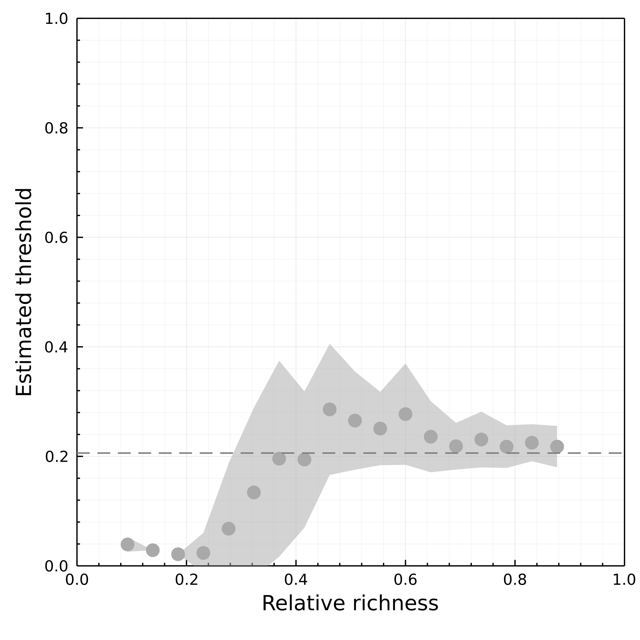
\includegraphics[width=\textwidth]{./figures/supplementary/sensibility_threshold_species.png}

More strikingly, looking at the rates of true/false positive/negative,
as illustrated below, it is clear that RDPG can be thresholded in a way
that yields an almost perfect classifier:

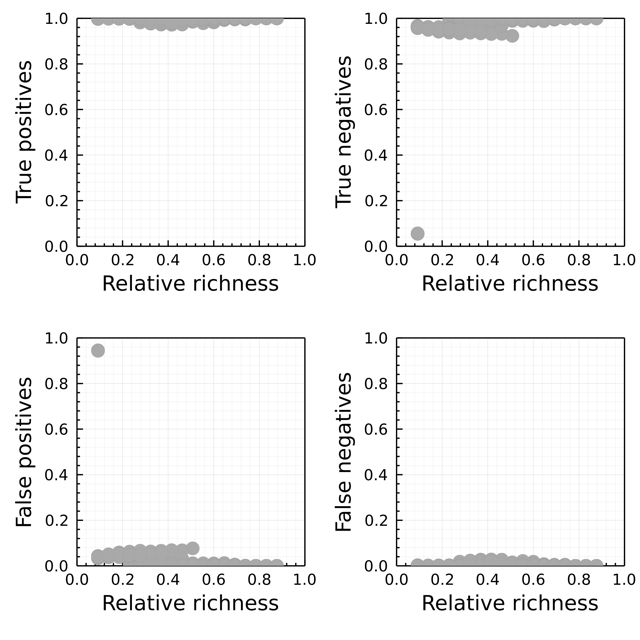
\includegraphics[width=\textwidth]{./figures/supplementary/sensibility_species.png}

These results may be surprising, given that ecological models usually do
not reach this degree of accuracy. That being said, we use the first 12
ranks of the network to approximate it, and this contains a lot of
information; in short, the minute discrepancies between the predictions
and the actual data can be attributed to leftover noise in the original
dataset.

\subsection{RDPG recovers withheld
interactions}\label{rdpg-recovers-withheld-interactions}

RDPG is able to correct almost all \emph{added} interactions (added
interactions were \emph{not} originally present in the European metaweb
and could be seen as introducing false positives to the data), which is
very strong evidence that the metaweb produced using it are not going to
contain too much spurious interactions. When \emph{removing}
interactions (\emph{i.e.} introducing false negatives to the data), even
when half are missing, RDPG was able to accurately reconstruct about 75
to 80\% of them. Predictably, the performance when both adding and
removing interactions is in between the two scenarios.

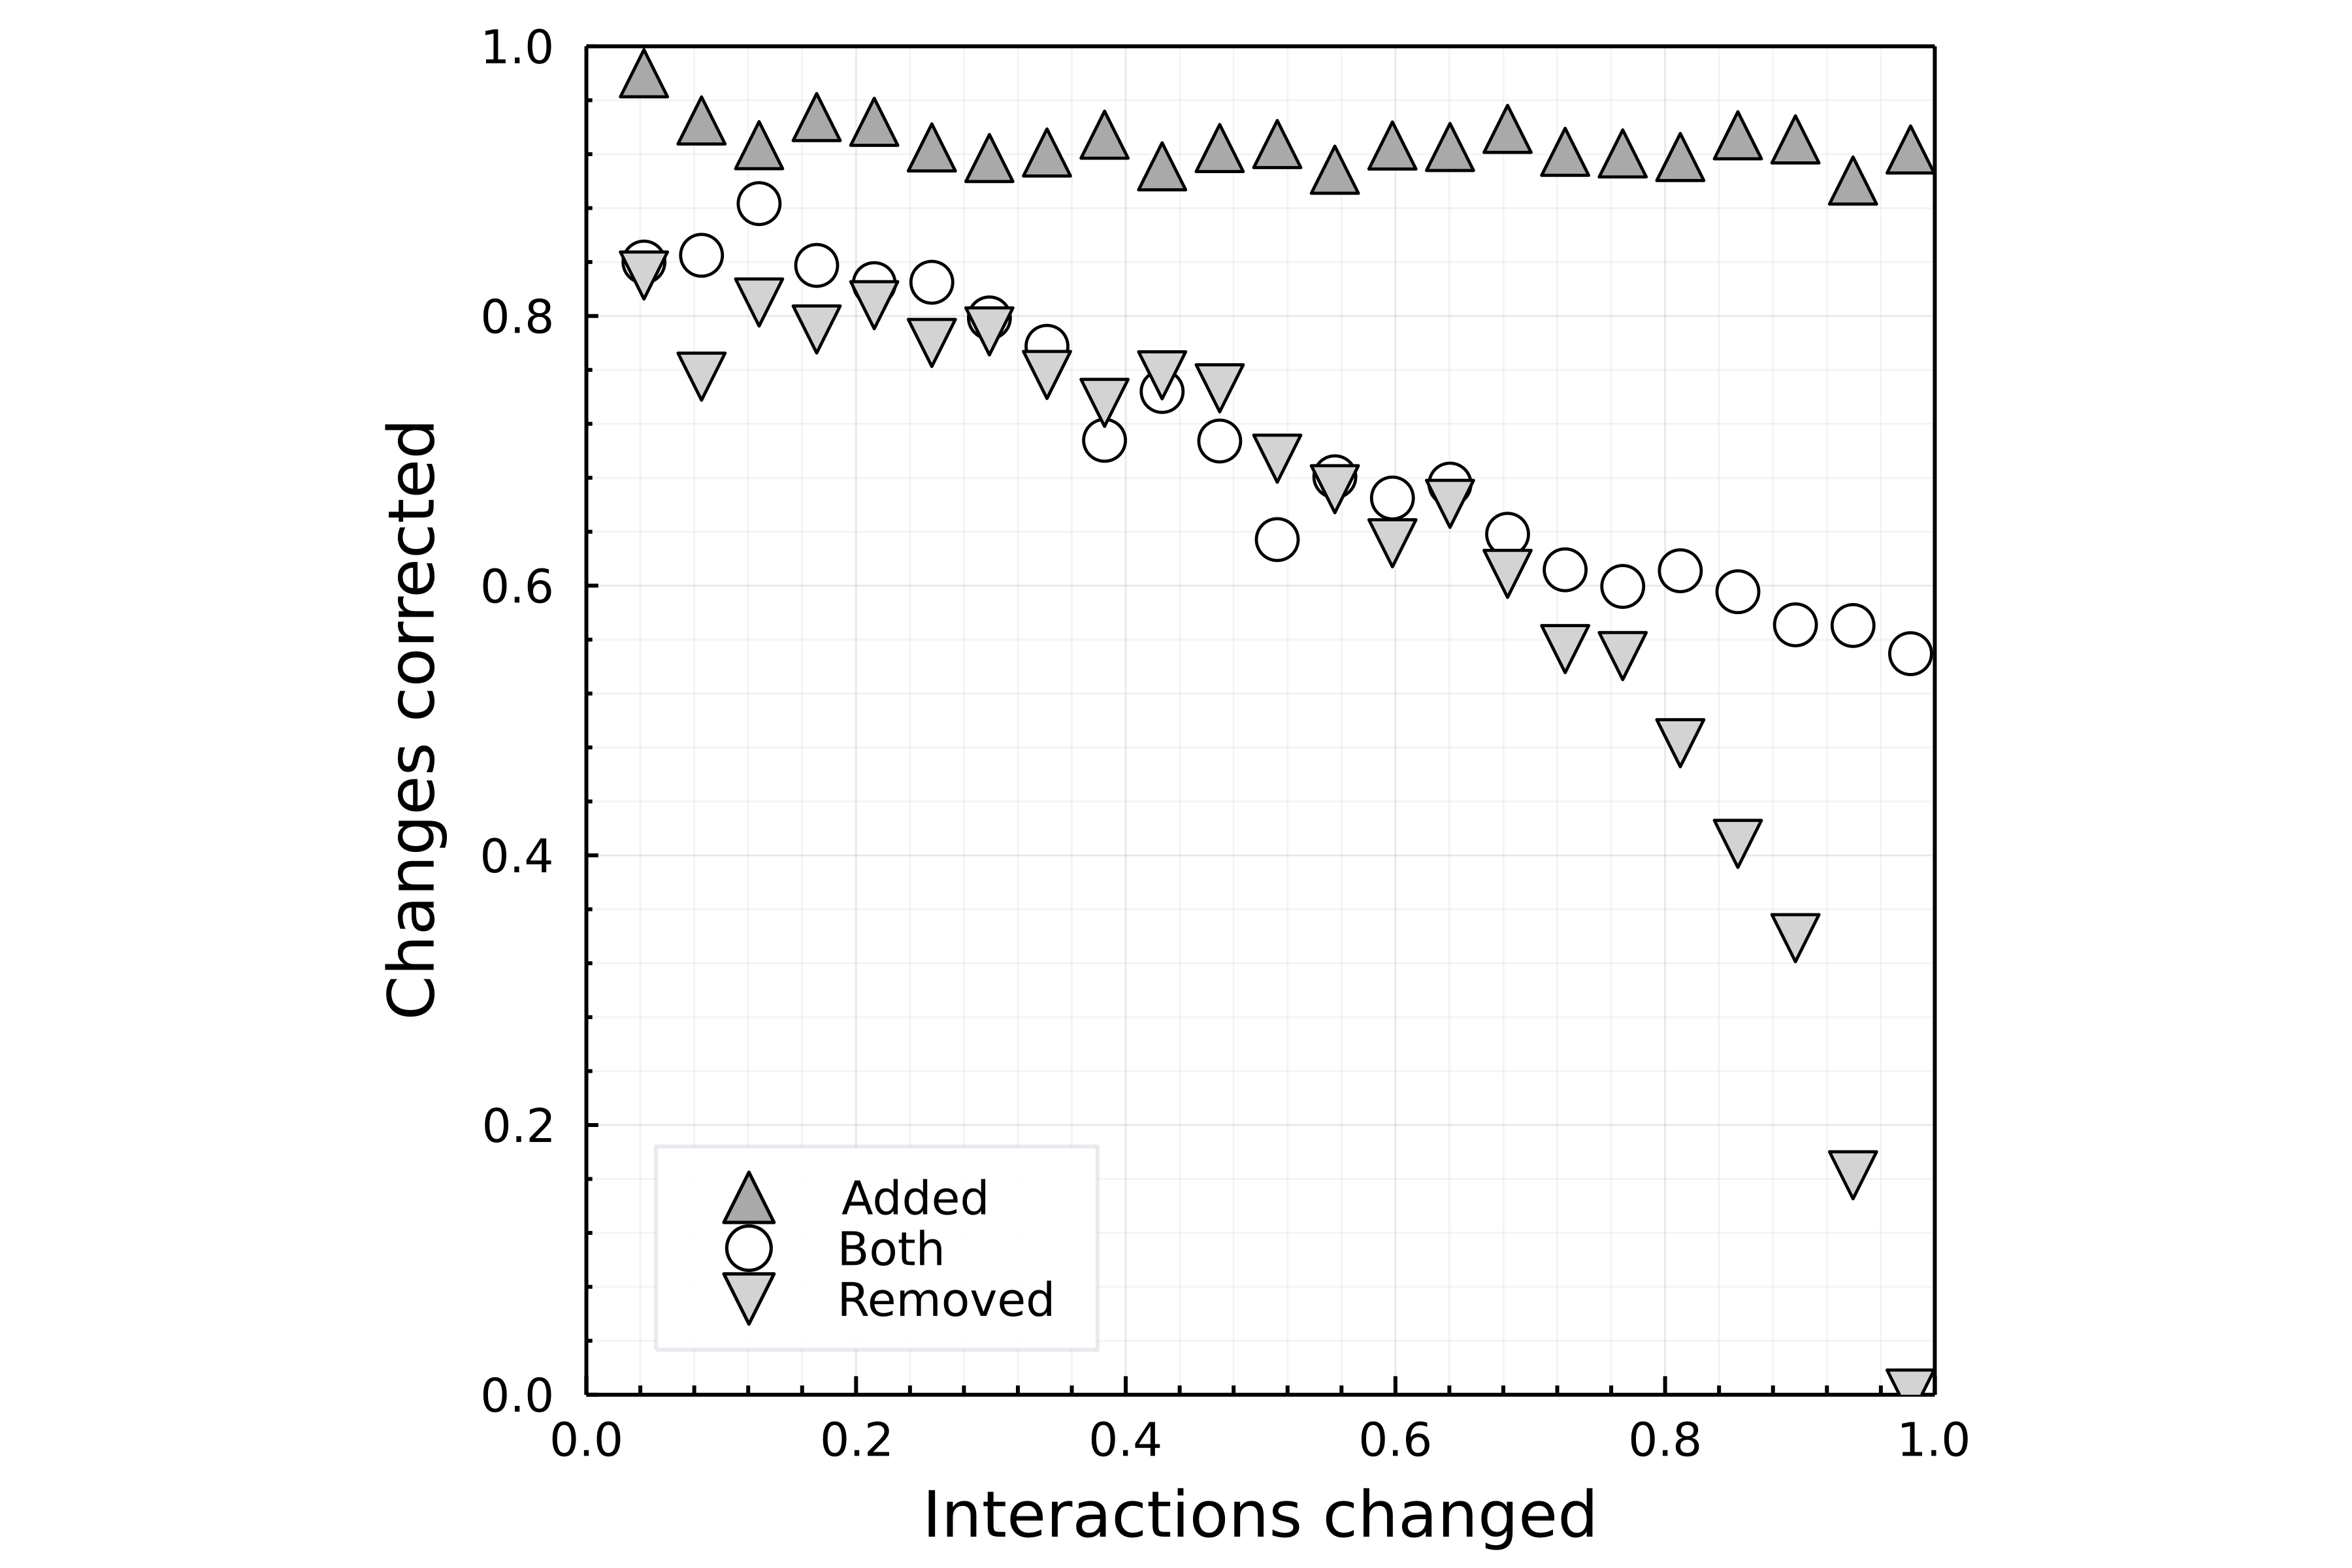
\includegraphics[width=\textwidth]{./figures/supplementary/sensibility_recovery.png}

The stochasticity in the proportion of recovered interactions is larger
when a small number of interactions are withheld, which makes sense as
the \emph{number} of interactions is far smaller (compared to the
overall network size).

Next, it is interesting to note that the threshold ``adapts'' to the
amount of missing information - the dashed line corresponds to the
threshold we used in the manuscript. Adding interactions specifically
did not result in an increase in the threshold, further suggesting that
RDPG is extremely good at removing spurious interactions.

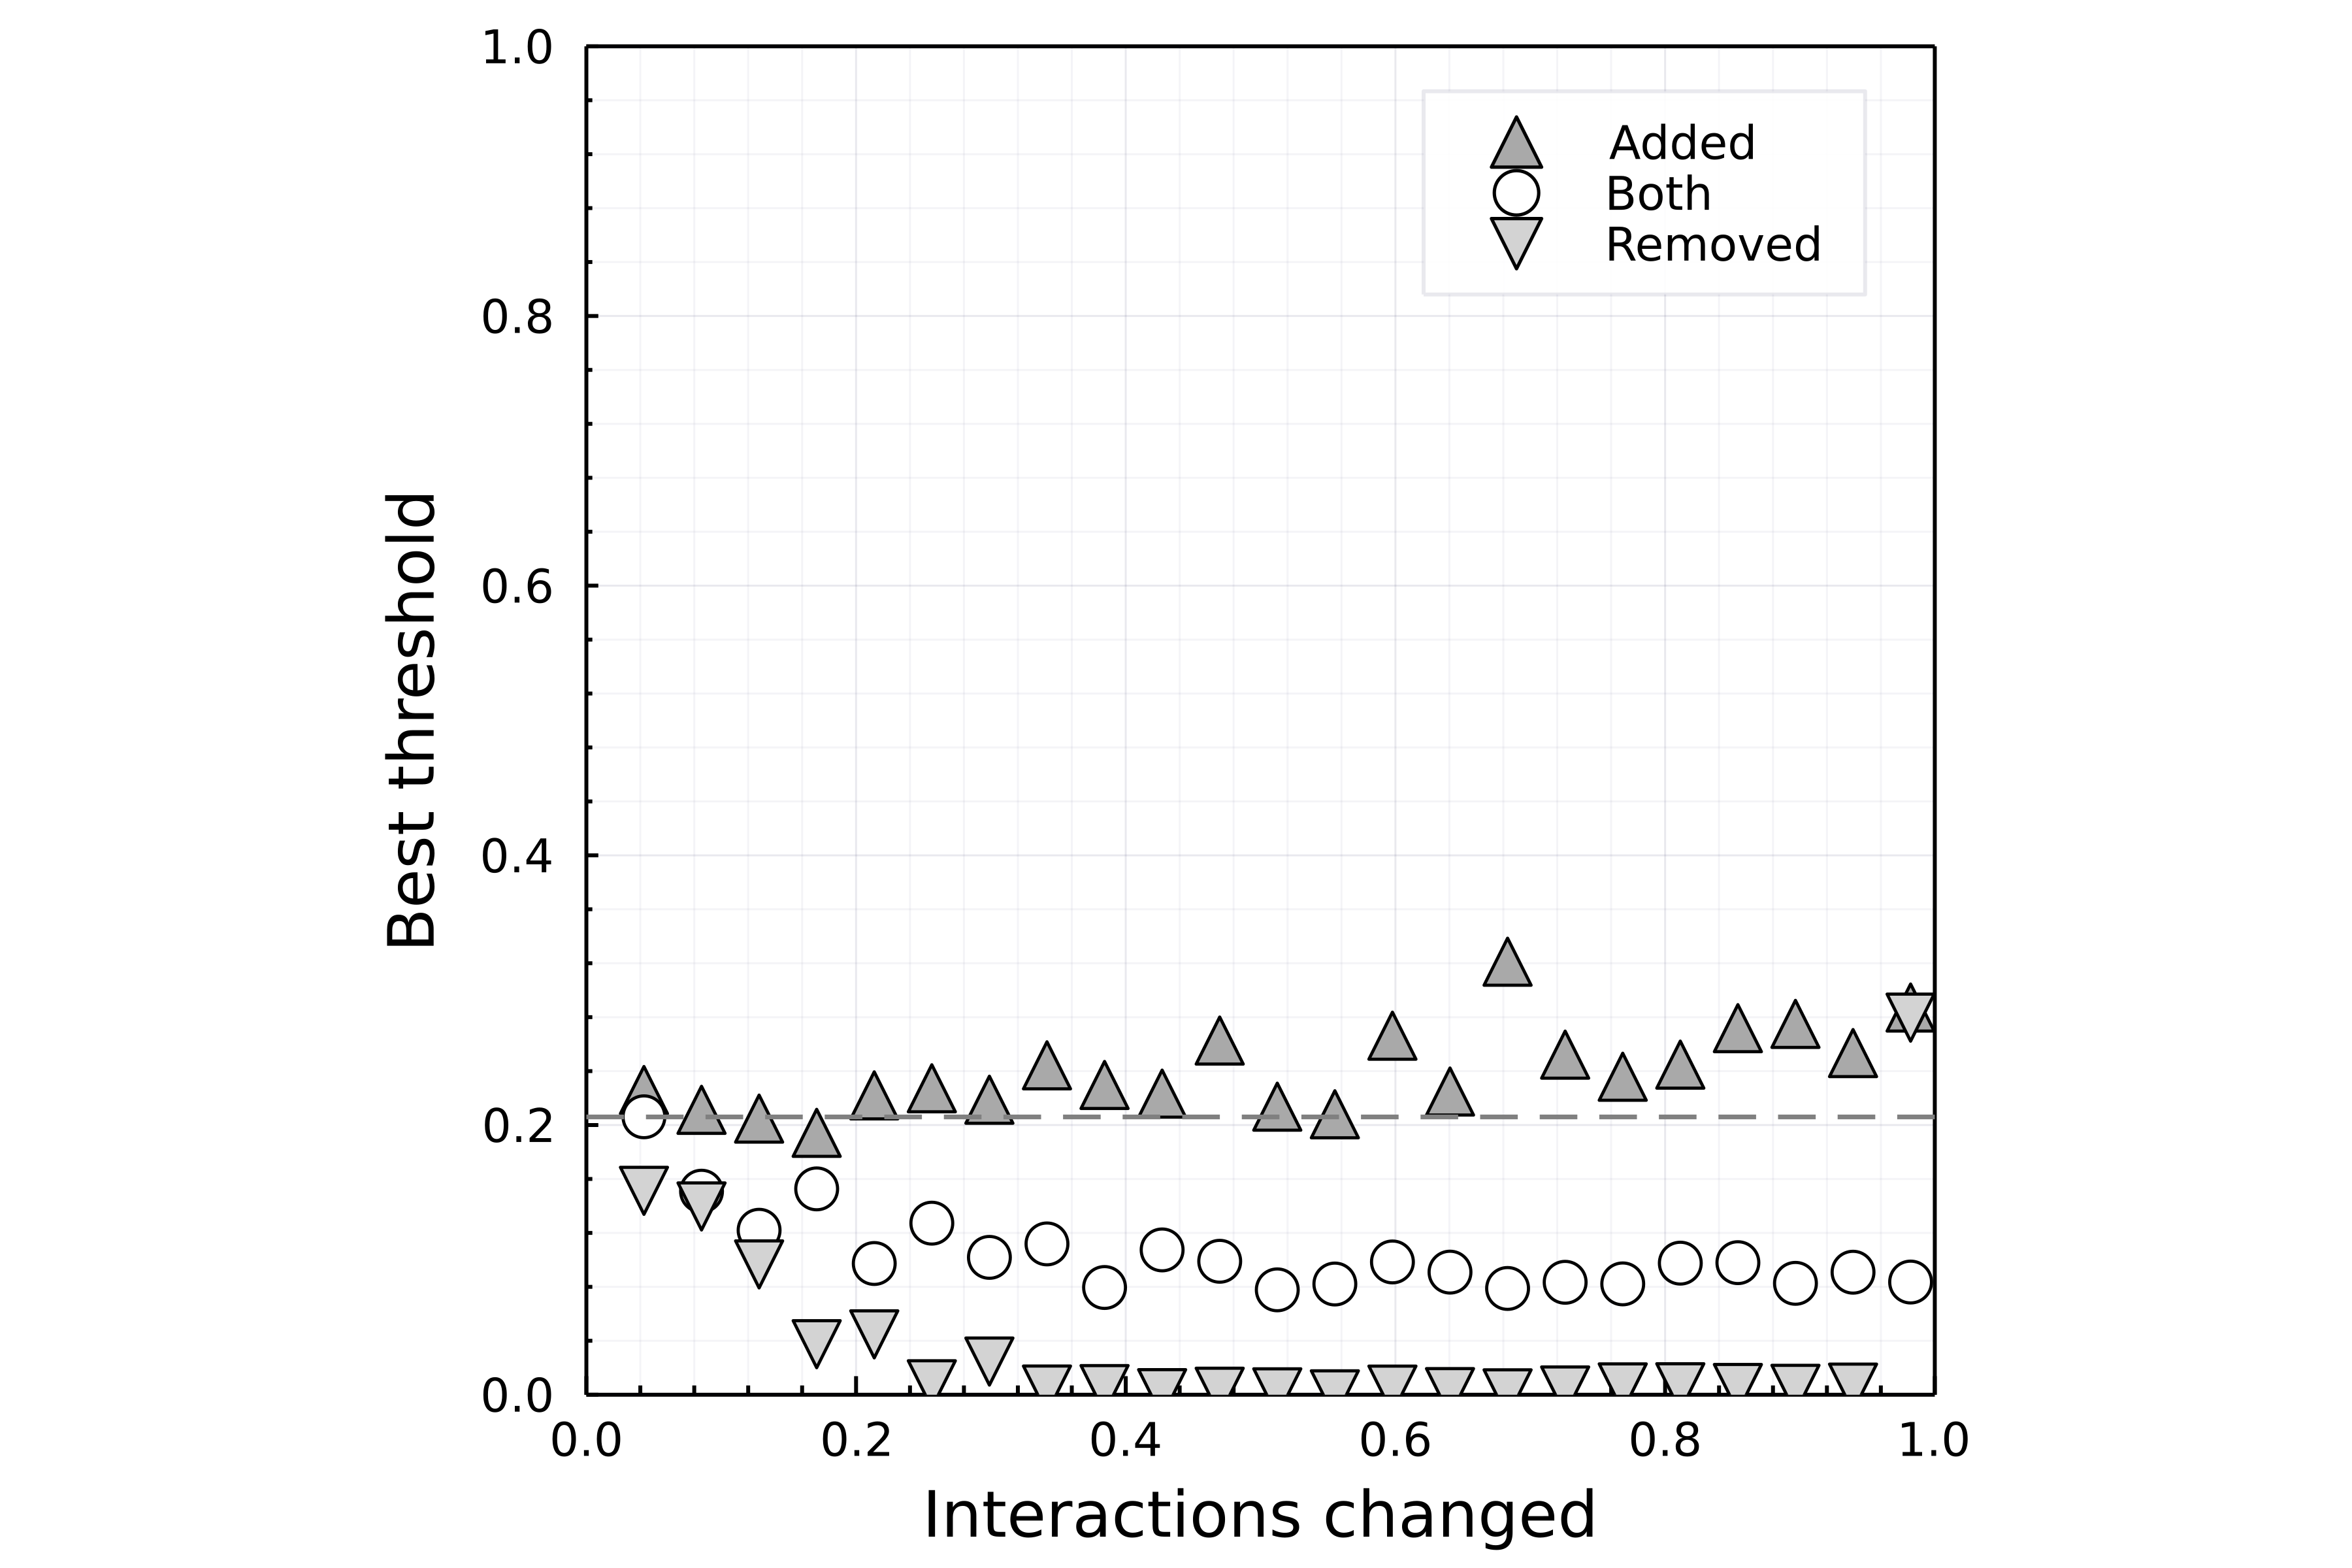
\includegraphics[width=\textwidth]{./figures/supplementary/sensibility_threshold.png}

The important consequence of this result is that training the RDPG on a
sub-sample of the network (\emph{i.e.} one missing interactions) would
result in a lower threshold, thereby potentially creating more false
positives when applied to novel data; this further justifies our
decision to use the entire evidence to estimate the threshold.

\subsection{RDPG yields an accurate
classifier}\label{rdpg-yields-an-accurate-classifier}

More important than the recovery of removed interaction is the fact that
the classifier should have a good global performance. One measure to
assess this is the area under the receiving operator characteristic
curve, or ROC-AUC. By this measure, the RDPG remains an excellent
classifier even if 50\% of interactions are withheld, and no matter what
the amount of changes are made by adding or both adding and removing
interactions.


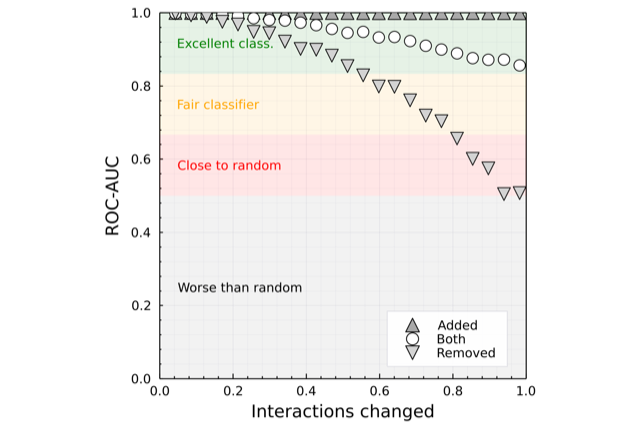
\includegraphics[width=\textwidth]{./figures/supplementary/sensibility_rocauc.png}

The overall agreement between a classifier and the actual data can be
measured by Cohen's \(\kappa\), which gives a similar result.

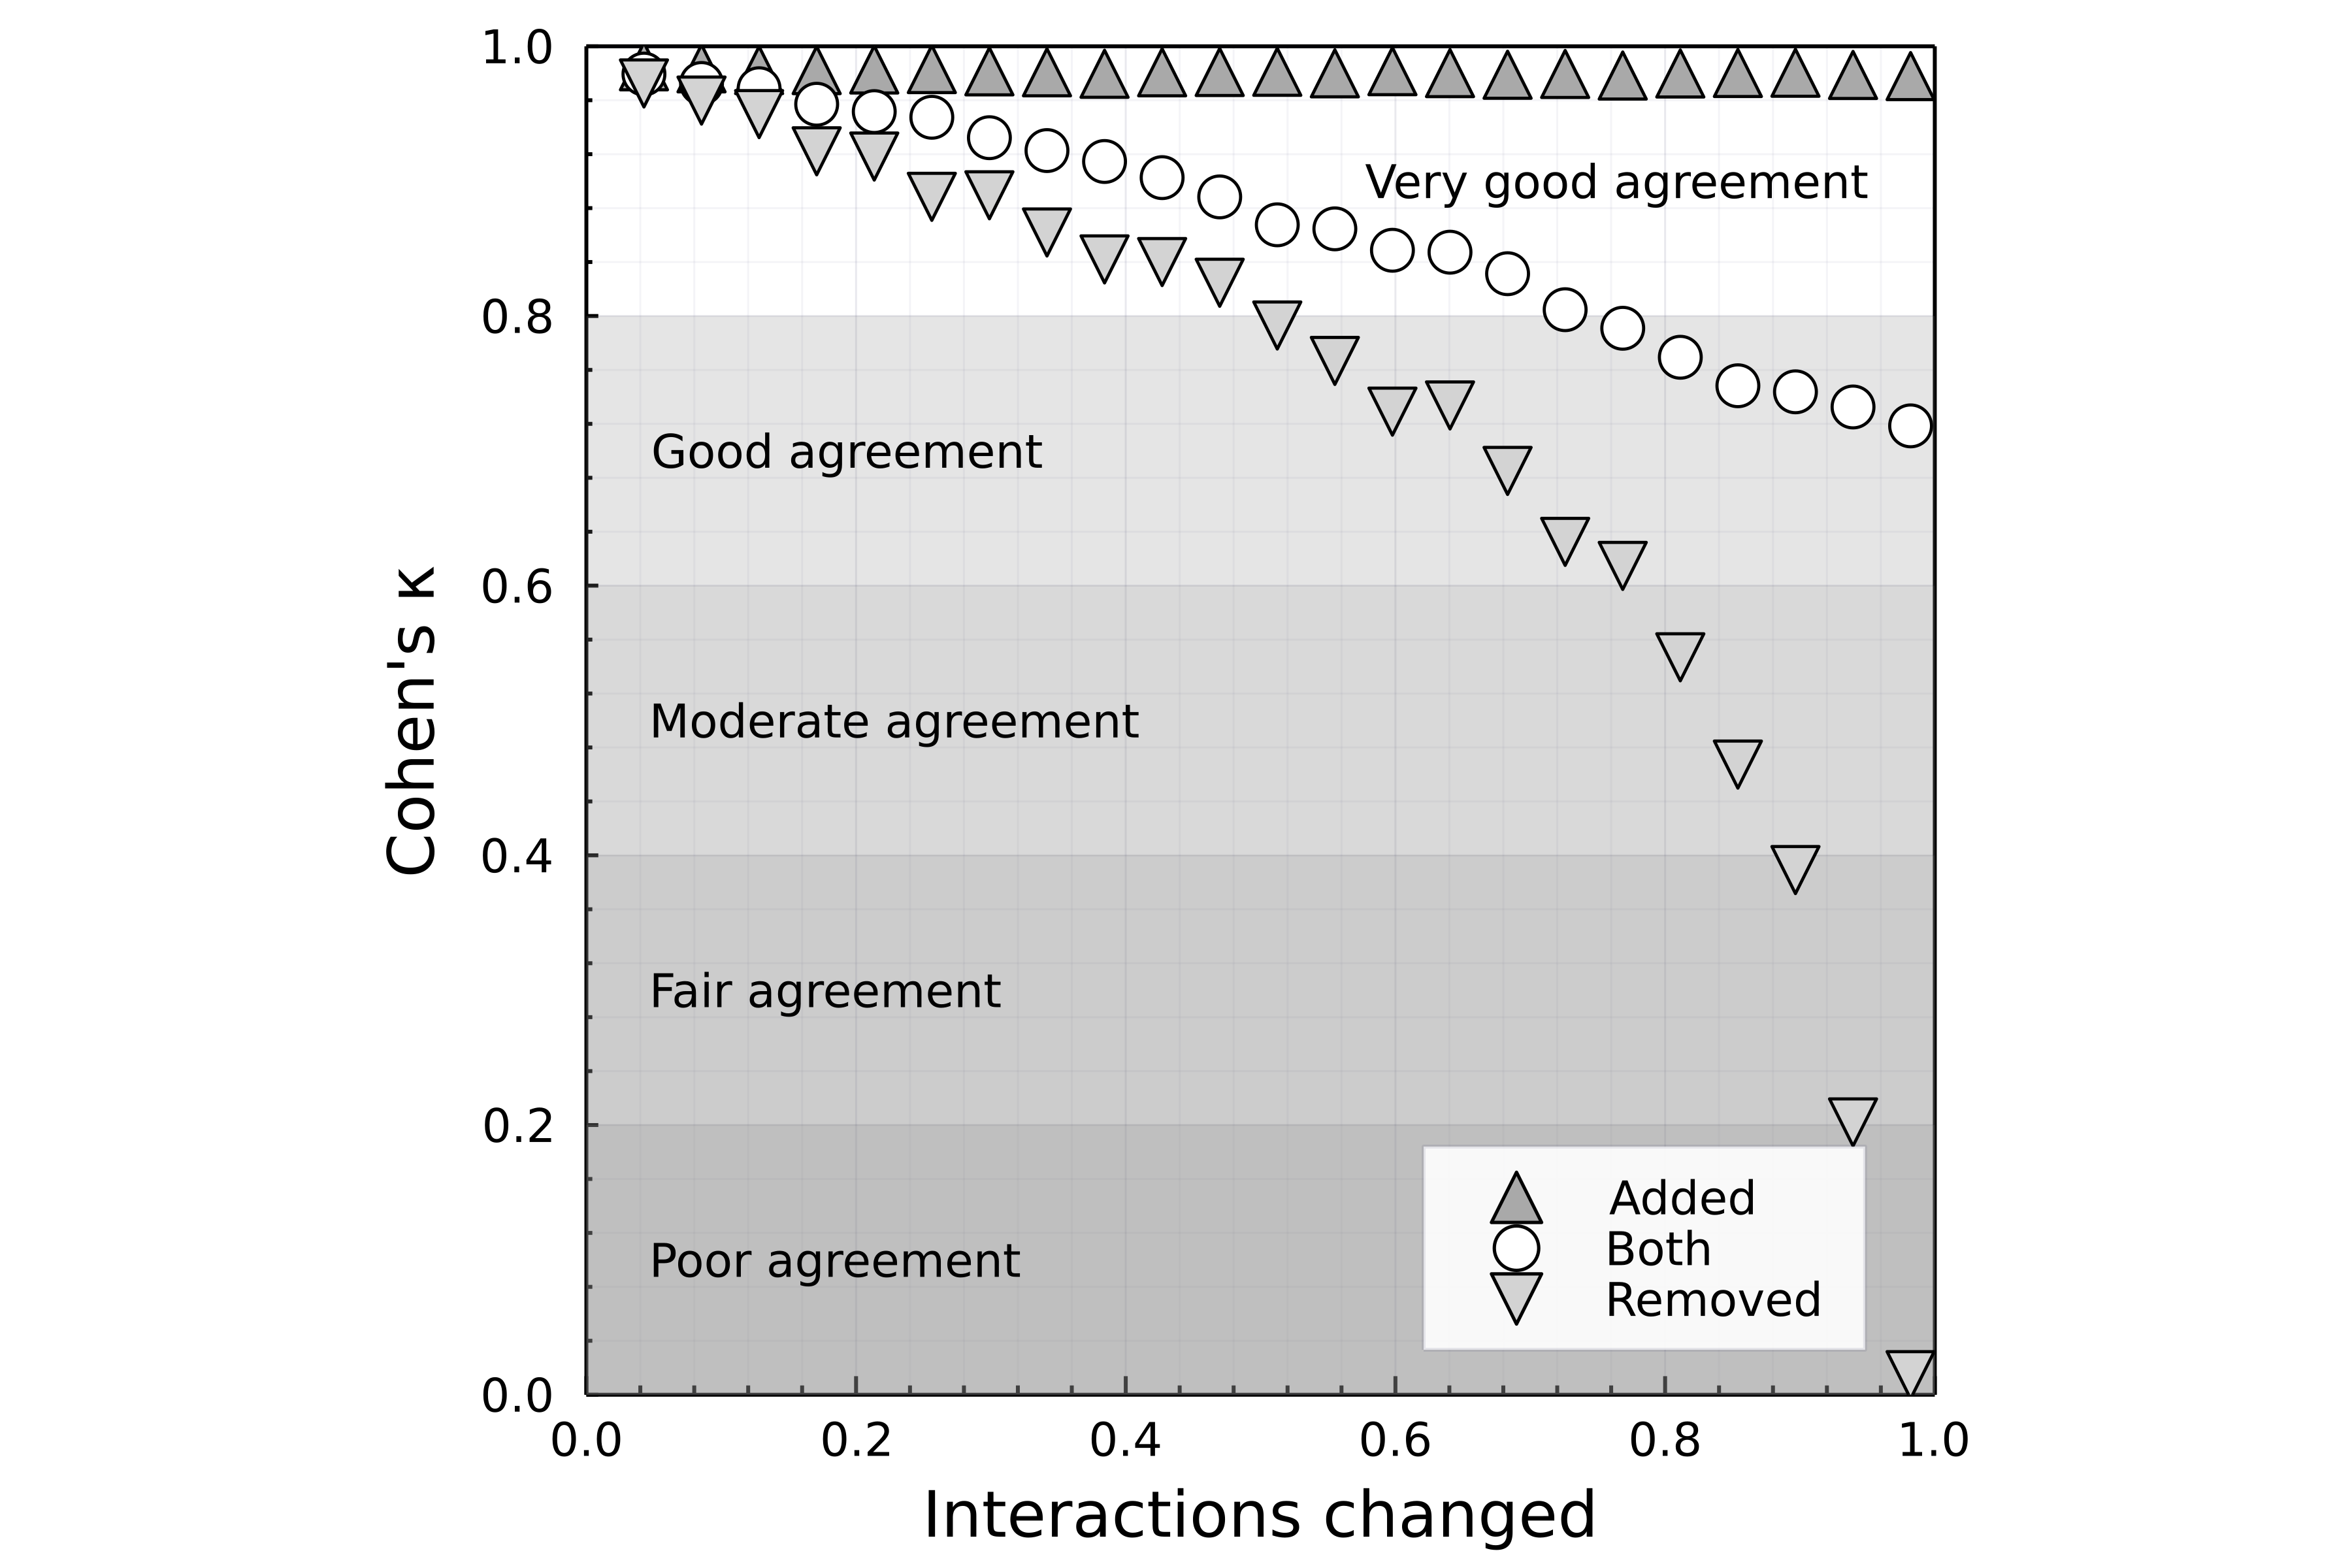
\includegraphics[width=\textwidth]{./figures/supplementary/sensibility_kappa.png}

These two diagnostic figures reveal that, although we used a probably
exhaustive list of interactions to do the initial RDPG, there are
chances that the approach would work on less complete datasets.

\subsection{RDPG recreates ecologically realistic
networks}\label{rdpg-recreates-ecologically-realistic-networks}

In this section, we present the relationship between the empirical
measure of the network structure (dashed line) and the reconstructed
estimate based on RDPG after the optimal threshold has been applied. We
focus on connectance (for its broad relevant to food web structure)
first:

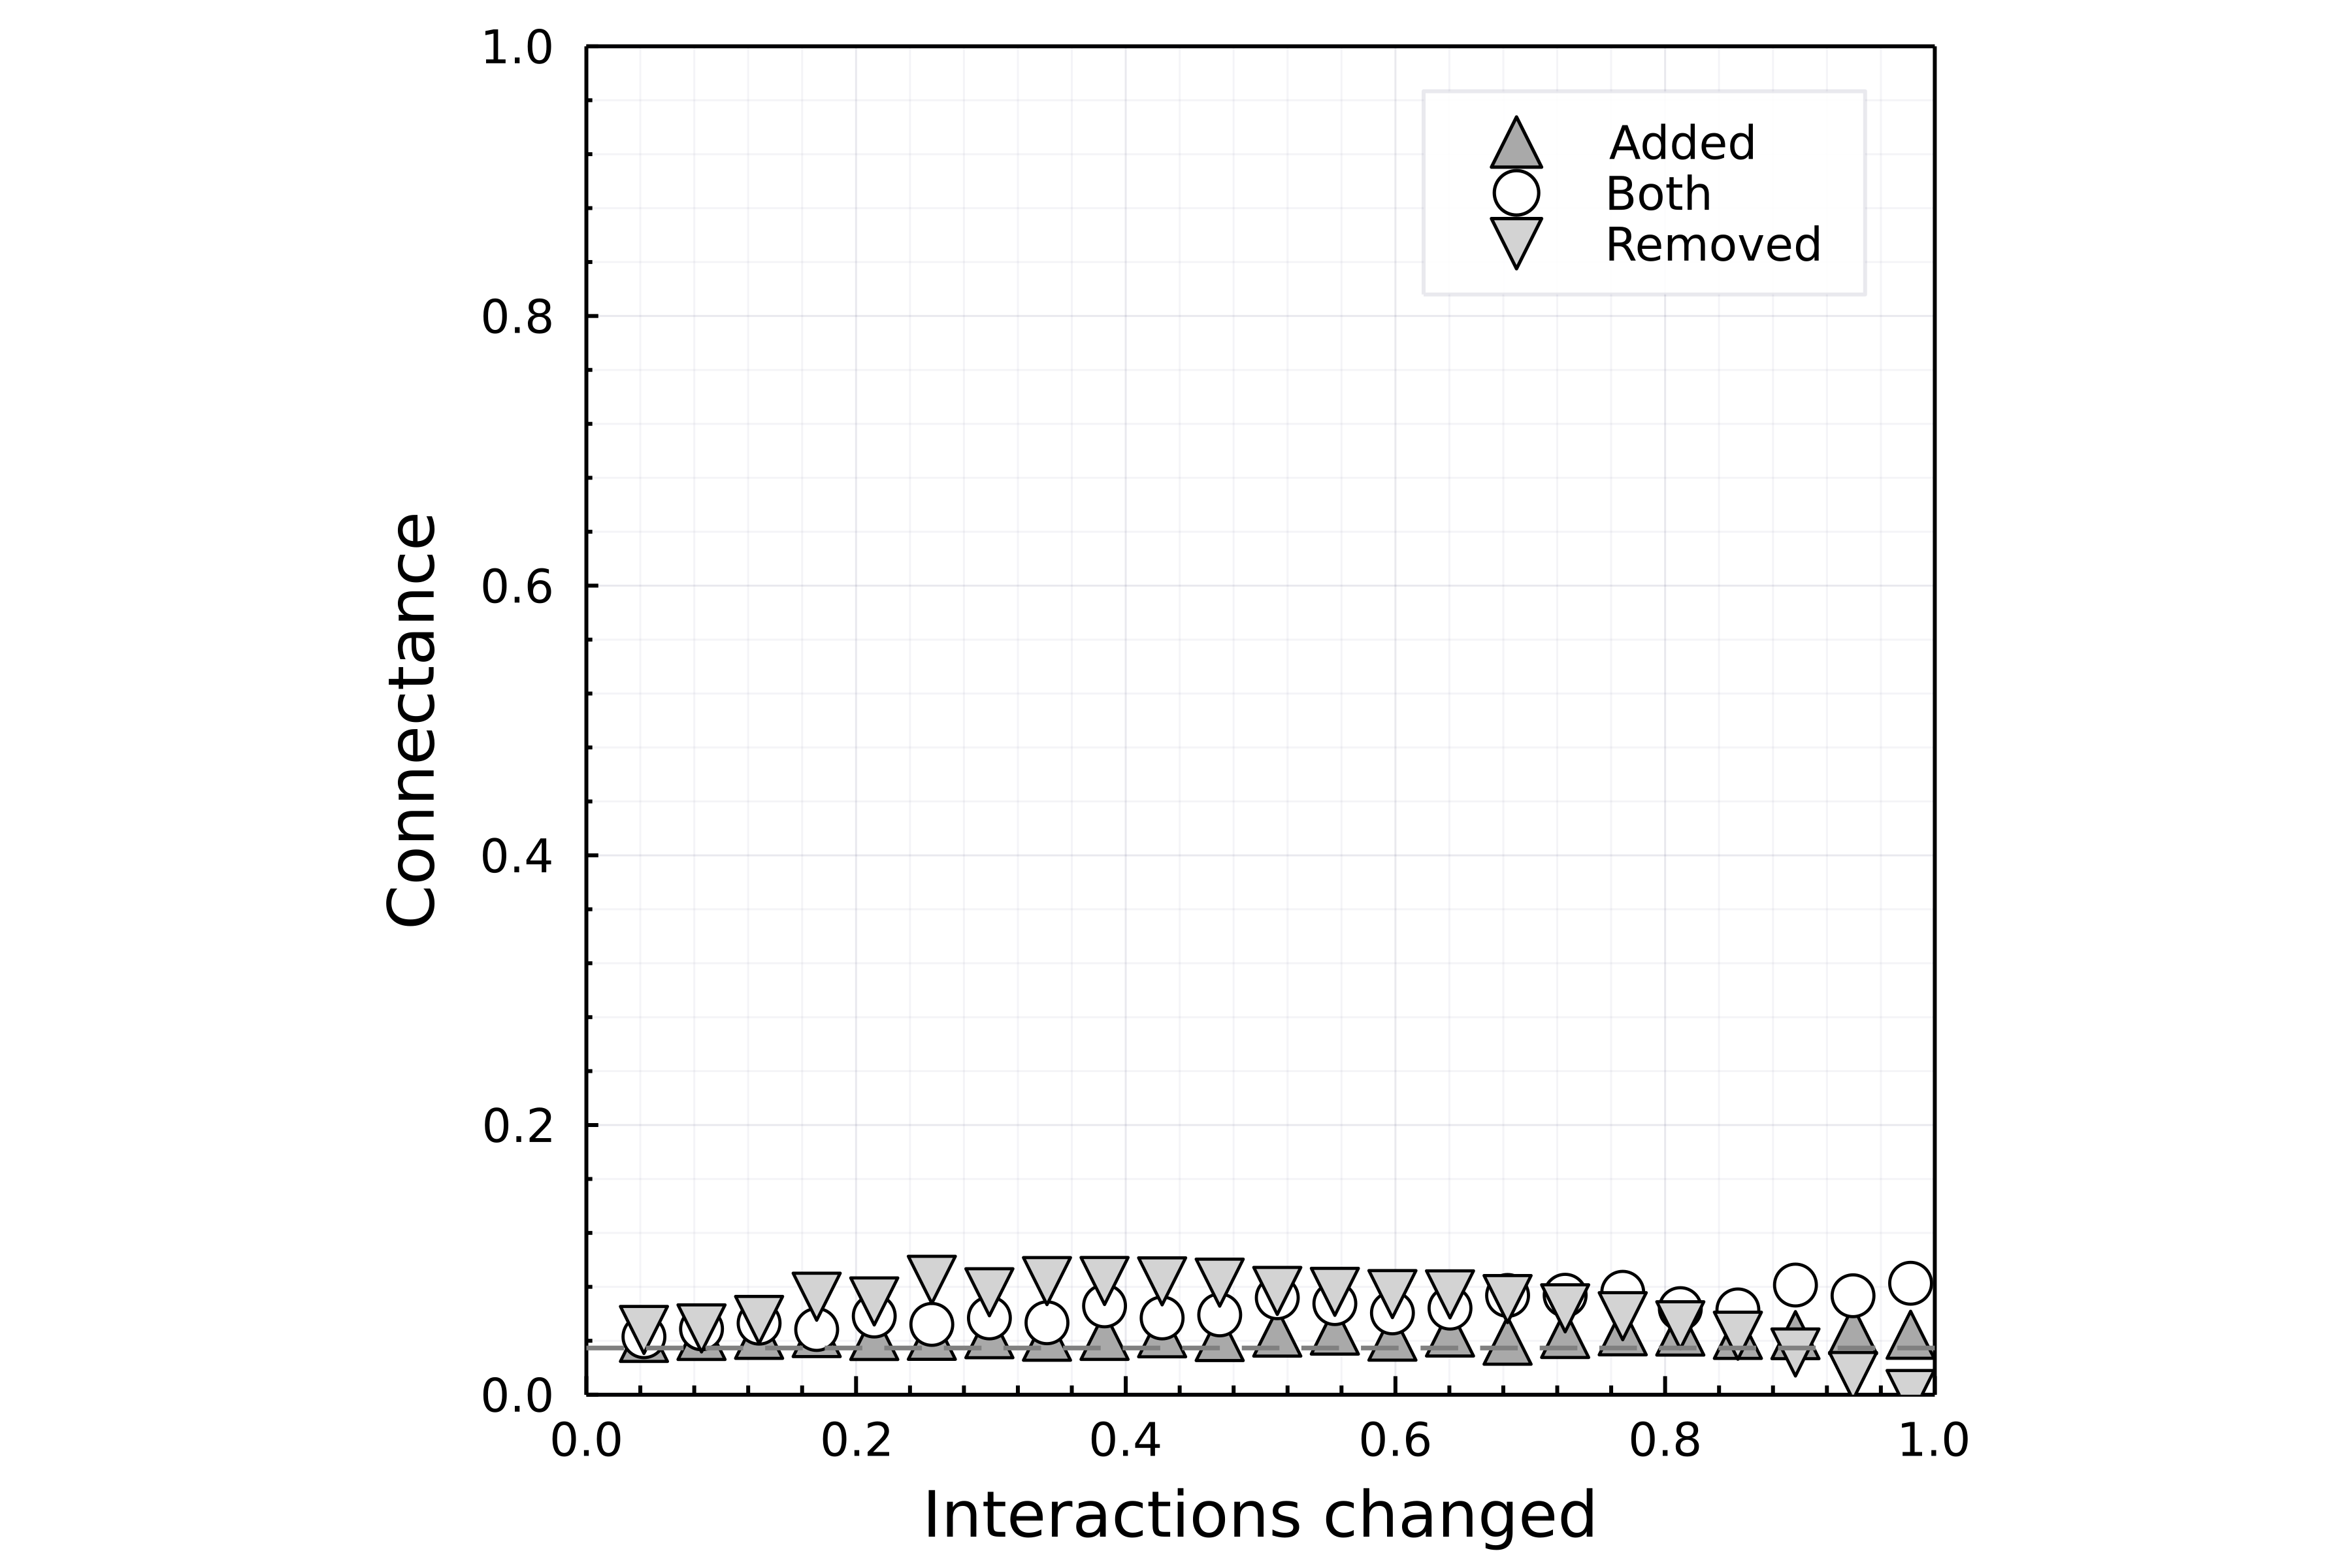
\includegraphics[width=\textwidth]{./figures/supplementary/sensibility_connectance.png}

Connectance increases slightly when initial information is incomplete,
but saturates at a value of around 0.12 -- this is still within the
bounds of connectances expected for food webs.

Next, we look at the ratio between direct competition
(\(a \rightarrow (b,c)\)) and apparent competition
(\((a,b) \rightarrow c\)) motifs, as motifs are known to be conserved
blocks in food webs:

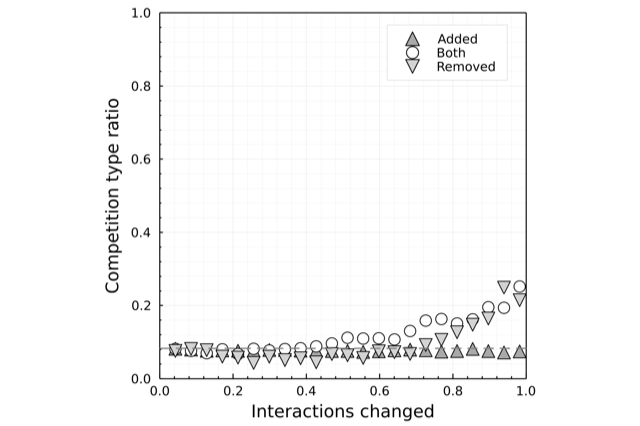
\includegraphics[width=\textwidth]{./figures/supplementary/sensibility_motifs.png}

This ratio remains close to the real one up until 75\% of initial
interactions are modified.

\subsection{Consequences}\label{consequences}

Based on these results, applying RDPG on the entire European network is
reasonable, especially since (i) the threshold is insensitive to the
number of withheld species, and (ii) removing interactions would
artificially lower the threshold. Interestingly, the RDPG remains an
excellent binary classifier even in the face of strong data
modifications, which suggests that our framework can be used even in the
absence of a complete metaweb. Even more importantly, the addition of
wrong interactions to the original dataset was never an issue for the
RDPG classifier, which was almost always able to remove them.

\section{The Normal model of latent variable evolution
over-predicts}\label{the-normal-model-of-latent-variable-evolution-over-predicts}

In this appendix, we compare the raw predictions made by the Normal and
Uniform models of latent variable evolution. The Normal model was
created by (i) getting the average \(\mu\) of the simulated values for
each species/variable combination, and (ii) estimating the standard
deviation as \((\mu+c - \mu-c)/3.92\), where \(c\) is one half of the
95\% confidence interval around \(\mu\) divided by 3.92

As can be seen on the following figure, the Normal model tends to assign
high probabilities (up to \(p \approx 0.4\)) for interactions that the
Uniform model essentially rules out:

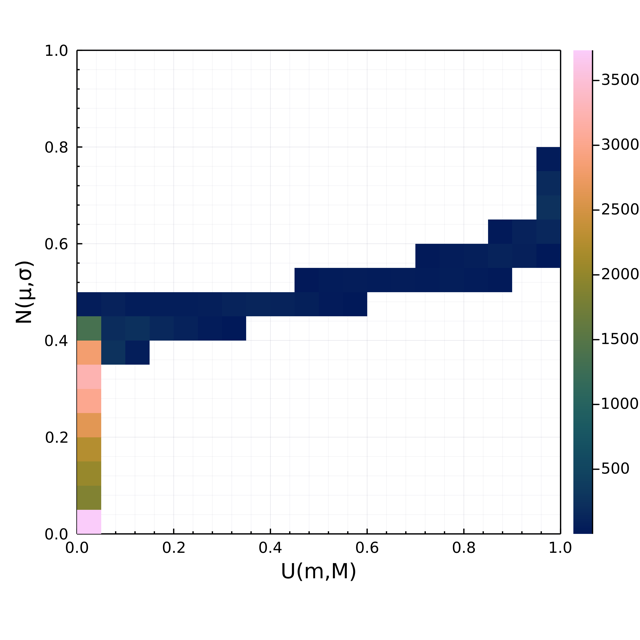
\includegraphics[width=\textwidth]{./figures/supplementary/comparison_models.png}

This can lead to severe over-estimation of the number of interactions.
In fact, the consequences of using a Normal model are obvious from
looking at the adjacency matrices below: most of the interactions are
predicted between species that occupy the lower trophic level, and are
ecologically unrealistic.

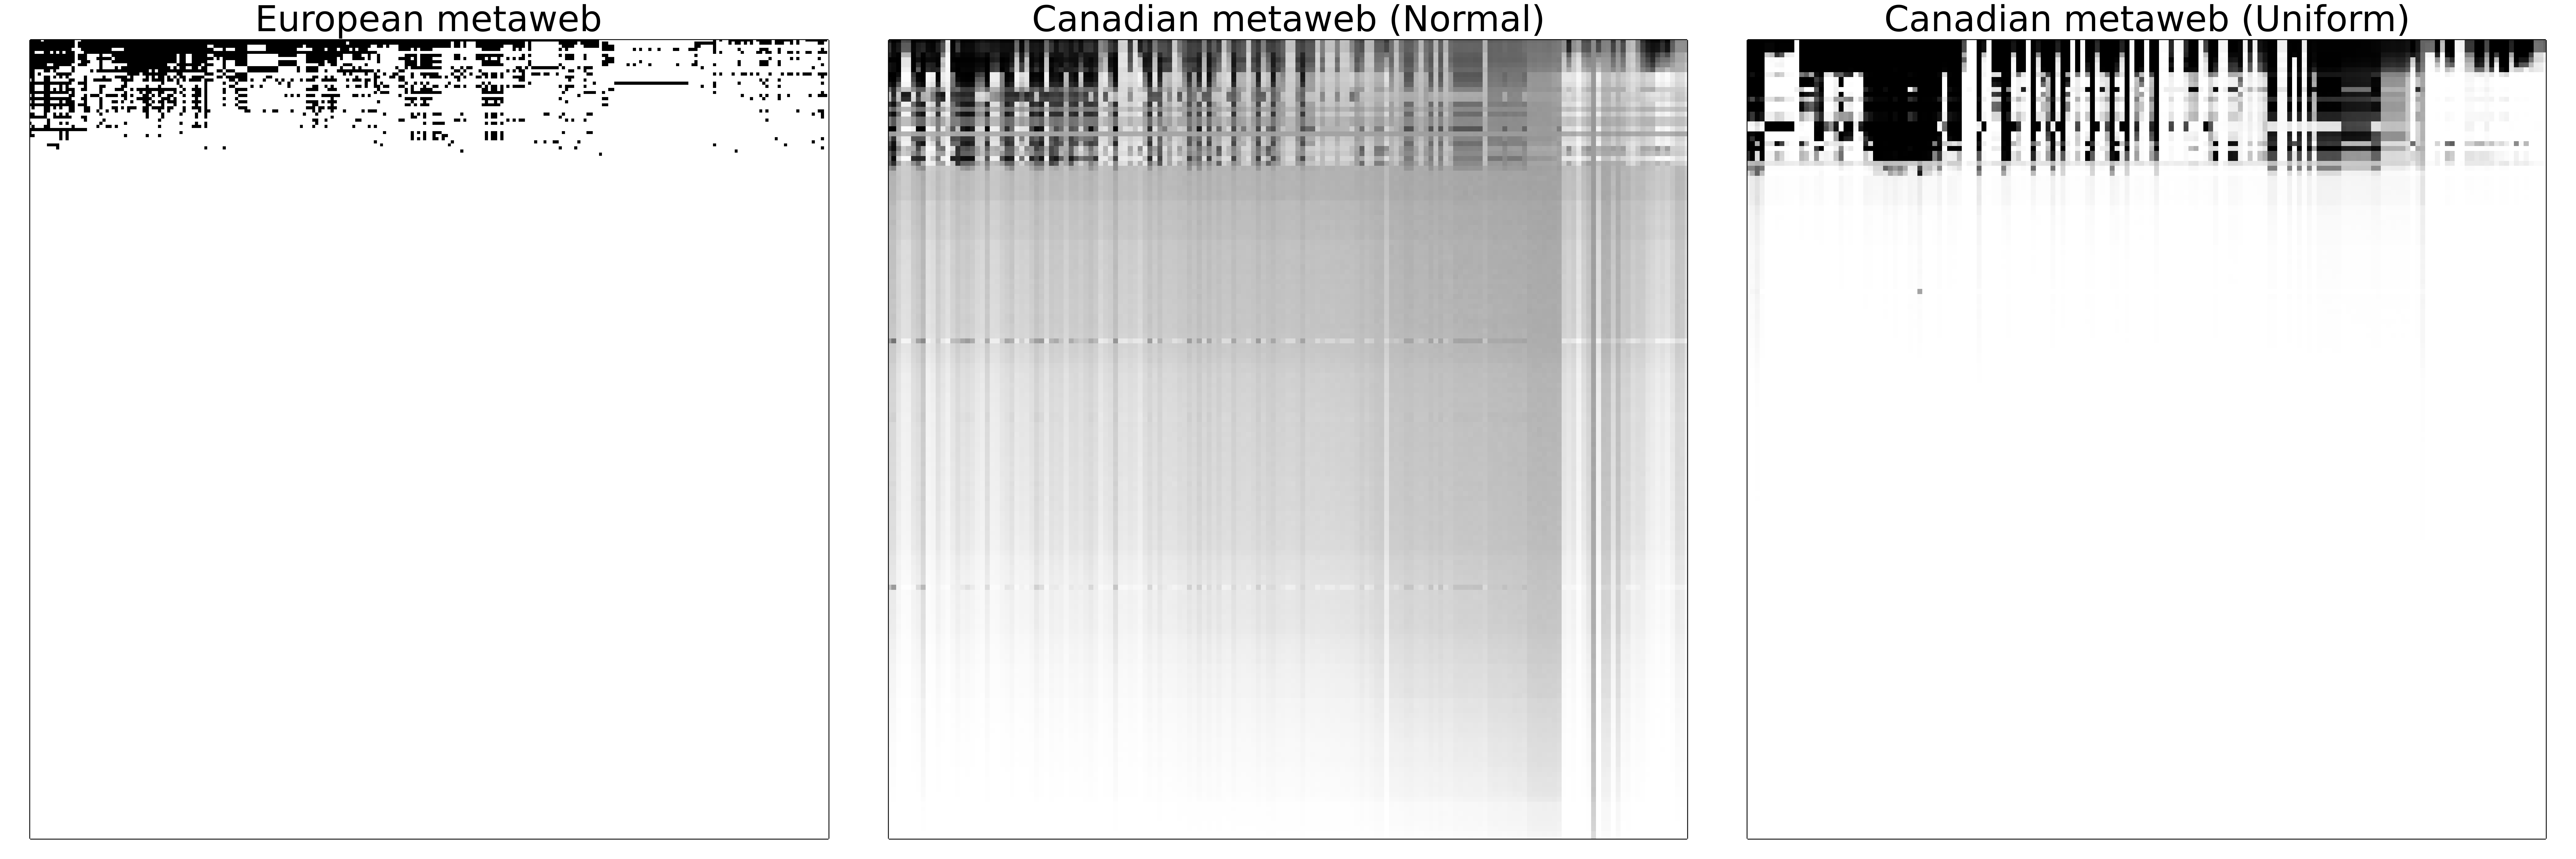
\includegraphics[width=\textwidth]{./figures/adjacencymatrices.png}

This can be further revealed by looking at the connectance of the
networks under different thresholds:

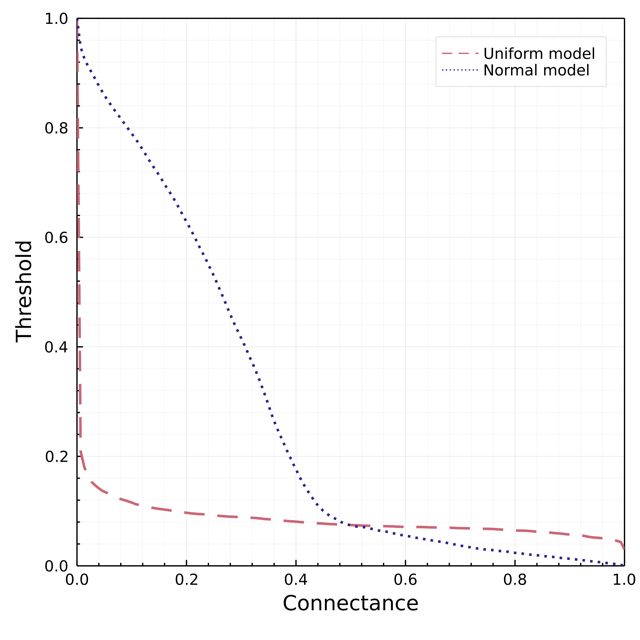
\includegraphics[width=\textwidth]{./figures/supplementary/comparison_connectance.png}

Although the Uniform model predicts a lot of interactions with extremely
low probability, that are removed at a low threshold, the distribution
of probabilities under the Normal model leads to extremely (abnormally)
high connectances even for thresholds that are over twice as large as
the optimal threshold determined in main text and Supp. Mat. 1.

This has consequences for the overall network \emph{structure}:
specifically, the Normal model predicts a lot more top predators than we
expect under the uniform model; rather than there being a progressive
change in top-intermediate-bottom proportions as the threshold changes,
there is an abrupt shift at a threshold of about 0.6, which suggests
that the Normal model is biased towards over-predicting most
interactions with probabilities in the range \([0,0.6]\).

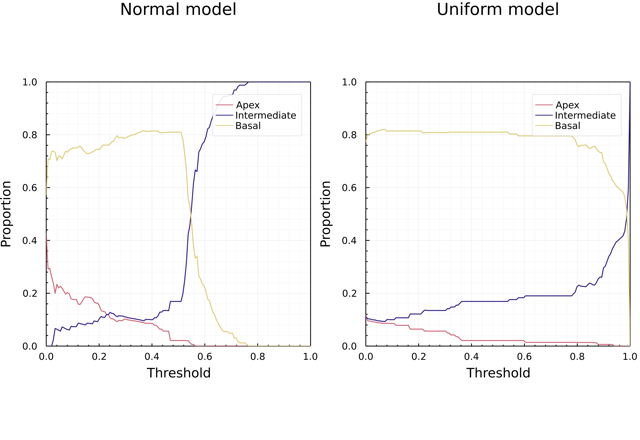
\includegraphics[width=\textwidth]{./figures/supplementary/comparison_tib.png}

The same ``jump'' can be observed when looking at the distribution of
food chain lengths:

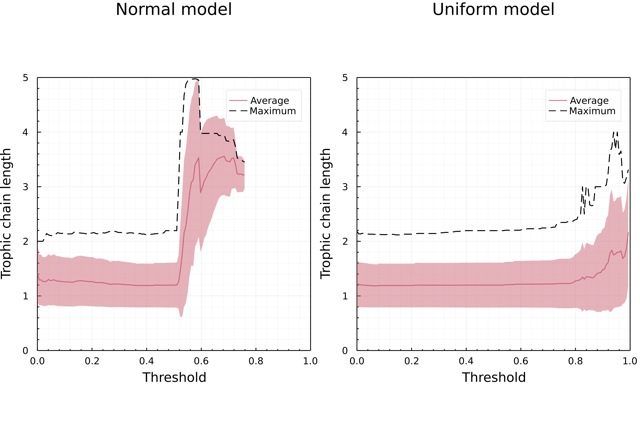
\includegraphics[width=\textwidth]{./figures/supplementary/comparison_rophicchain.png}

For these reasons, we only use predictions from the Uniform model in the
main text.

\section{RDPG reconstructed networks have diverse
structures}\label{rdpg-reconstructed-networks-have-diverse-structures}

In this appendix, we check that the networks reconstructed from the RDPG
do keep a variety of structural components, especially when selecting a
small species pools from within them. In order to do so, we induced 400
random subgraphs containing between 30 and 70 species, both from the
Canadian and European metawebs. For each of these subgraphs, we measured
eight variables: the mean and standard deviation of trophic levels, the
standard deviation of degree (total, in, and out), and the proportion of
top, intermediate, and basal species. We selected a random subset of 300
rows from the network-property matrix to fit a Principal Component
Analysis projection matrix (\(W\)), which we then used to project all
networks into the space formed by the first two principal components.

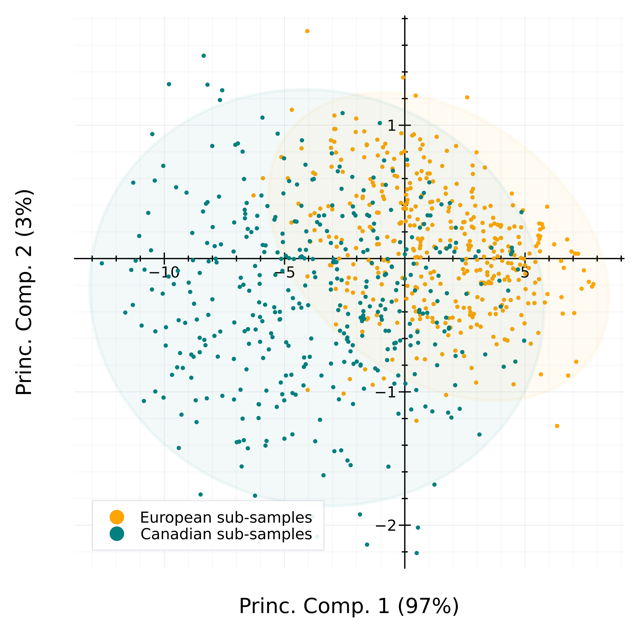
\includegraphics[width=\textwidth]{./figures/supplementary/variation_pca.png}

The first axis (explaining most variance) was strongly correlated to the
standard deviation of the number of preys (-0.71), and the second axis
to the standard deviation in the number of predators (-0.95). These
results match the conclusions in main text, namely that the first
dimensions of network embedding capture the degree distribution.

Two things are important to note on this representation; each point is
an induced sub-graph, and the ellipses are the 95\% confidence interval
around the points. First, there is some variations \emph{within} a group
(Europe \emph{v.} Canada); second, the two groups do not fully overlap.
This suggests that not only the sub-samples of the Canadian metaweb are
not equivalent to the sub-samples of the European metaweb (\emph{i.e.}
the two networks have structural differences), realizations (here in the
form of random local species pools) of the Canadian metaweb also show
some variability; in short, reconstructing a metaweb using a RDPG will
not result in homogeneous local networks, and may therefore be suitable
for lower-scale predictions.
\anglais
\doublespacing
\chapter{Supplementary material for \autoref{Perspectives}}\label{supp:perspectives}

The associated materials for this appendix is in the form of a Jupyter notebook file (a web-based interactive computing platform). At the time of writing the published article was not yet available online and thus this appendix will point to the notebook file that was associated with the GitHub repository associated with this chapter. The \emph{.ipynb} file can be found \href{https://github.com/PoisotLab/ms_metaweb_perspectives/blob/main/notebooks/SupplementaryMaterial.ipynb}{here}. Note it is also possible to download this file and open it in a Jupyter application should you wish for a more interactive experience.
\anglais
\doublespacing
\chapter{Understanding where networks stop}\label{supp:boundaries}
\begin{refsection}

\section{Why boundaries are interesting}

As discussed in both Chapters~\ref{Perspectives} and \ref{SpatialBoundaries}
there is value in thinking about the existence of boundaries between networks, either from a prediction perspective (\emph{e.g.,} knowing at what scale to make predictions at) or from a more theoretical question of where do networks stop? Although this is discussed in more detail in \autoref{Defining-ecotrophic-zones} there is one question regarding network boundaries that might be a good starting point and that is looking at how environmental and network boundaries relate, more specifically do environmental changes drive changes in networks. Here I present what is more of a methodological framework (as opposed to an actual answer, hence why it has been relegated as an Appendix) that we can use to try and answer this question.

\section{A metacommunity model for boundary detection}

The metacommunity model developed by \cite{Thompson2017Dispersal} is a good starting point to use for this 'case study' as it allows us some flexibility with how we want to parameterise the system. The model (\ref{eq:metacomm_full}) itself is based on a tritrophic community ('plants', 'herbivores', and 'carnivores') and is a collection of modified Lotka–Volterra equations and (broadly) models species abundance as a function of interaction strength, environmental effect, immigration, and emigration. The metacommunity consists of $S$ species with $M$ environmental patches and looks as follows:

\begin{equation} \label{eq:metacomm_full}
X_{ij}(t+1)=X_{ij}(t)exp\left[C_{i} + \sum_{k=1}^{S}B_{ik}X_{kj}(t)+A_{ij}(t)\right]+I_{ij}(t)-X_{ij}(t)a_{i}
\end{equation}

Where $X_{ij}(t)$ is the abundance of species $i$ in patch $j$ at time $t$. $C_i$
is its intrinsic rate of increase (which we have set to 0.1 for 'plants' and
-0.01 for 'herbivores' and 'carnivores'). $B_{ik}$ is the per capita effect of
species $k$ on species $i$. The exact interaction strength for each species pair
is drawn from a uniform distribution with the parameters for the 
interaction pairs listed in \autoref{table:interaction_strength}, the values
drawn from the uniform distribution are scaled by dividing by $0.33S$ to yield
the final interaction strength for each interacting pair.

\begin{table}[h!]
\centering
\begin{tabular}{||c c||} 
 \hline
Interacting pair & Range of uniform distribution \\ [0.5ex] \hline\hline
 Plant-plant & -1 -- 0 \\ 
 Plant-herbivore & 0 -- 0.1 \\
 Plant-carnivore & 0 \\
 Herbivore-plant & -0.3 -- 0 \\
 Herbivore-herbivore & -0.2-- -0.15 \\
 Herbivore-carnivore & 0 -- 0.08 \\
 Carnivore-plant & 0  \\
 Carnivore-herbivore & -0.1 -- 0  \\
 Carnivore-carnivore & -0.2-- -0.15 \\ [1ex] 
 \hline
\end{tabular}
\caption{Intervals used for the uniform distribution from which interaction
strengths values are drawn from for the different types of species pair
interactions. Note this is represent the effect of species type 1 on species
type 2 \emph{i.e.,} herbivore-plant represents the effect of a herbivore species on a plant species}
\label{table:interaction_strength}
\end{table}

$A_{ij}(t)$ is the effect of the environment in patch $j$ on species $i$ at time $t$ and can be further expanded as follows:  

\begin{equation} \label{eq:metacomm_env}
A_{ij}(t)=h\left(exp-\frac{(E_{j}(t)-H_{i})^2}{2\sigma^2}-1\right)
\end{equation}

Species environmental optima ($H_i$) are evenly distributed across the entire range of environmental conditions for each trophic level, meaning that species from different trophic levels will be at, or near the same environmental optima. $h$ is a scaling parameter (set to 300), $E_j(t)$ is the environment in patch $j$ at time $t$ and $\sigma$ is the standard deviation (set to 50).

$I_{ij}(t) $is the abundance of species $i$ immigrating to patch $j$ at time $t$
and can be expanded as follows:

\begin{equation} \label{eq:metacomm_imm}
I_{ij}(t)=\sum_{l=j}^{M}a_iX_{il}(t)exp(-Ld_{jl})
\end{equation}

Where $ai$ is the proportion of the population of species $i$ that disperses at each time step, the dispersal rate is drawn from a normal distribution ($\mu$ = 0.1, $\sigma$ = 0.025) for each species. The abundance of immigrants to patch $j$ from all other patches is governed by where $d_{jl}$ is the geographic distance between patches $j$ and $l$, and $L$ (the strength of the exponential decrease in dispersal with distance), which is also drawn from a normal distribution for each species. The parameters used for $L$ are trophic level dependant and are show in \autoref{table:interaction_decay}

\begin{table}[h!]
\centering
\begin{tabular}{||c c c||} 
 \hline
Trophic level & $\mu$ & $\sigma$ \\ [0.5ex] \hline\hline
 Plant & 0.3 & 0.075 \\ 
 Herbivore & 0.2 & 0.05 \\
 Carnivore & 0.1 & 0.025 \\ [1ex] 
 \hline
\end{tabular}
\caption{Parameters for the normal distributions used to determine the dispersal
decay ($L$) for each species depending on its trophic level.}
\label{table:interaction_decay}
\end{table}

\section{A toy example of boundary detection}

The associated code for these simulations was carried out in \texttt{Julia 1.8} \cite{Bezanson2017Julia} using \emph{Makie.jl} (\cite{Danisch2021Makie}) and can be found in a GitHub repo \href{https://github.com/PoisotLab/Omnomnomivores}{\texttt{here}}. Note that the results presented here are supposed to represent a hypothetical result and it is not so much that there is ecological knowledge to be gleaned from the figure below but rather to showcase how we can approach the idea of boundary detection across landscapes. For the initial modelling exercise presented below we had 80 species ($S$) and a 200 by 200 landscape ($M$). This landscape is generated using \texttt{NeutralLandscapes.jl}, which allows the user to specify different landscape types \emph{e.g.,} one with a clear boundary, the landscape values are used to represent the environmental value for that patch.

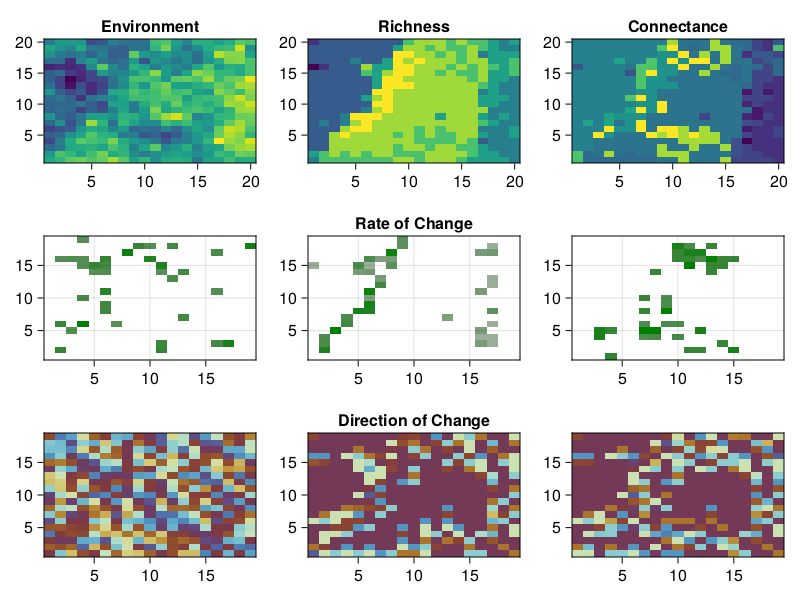
\includegraphics[width=\textwidth]{./figures/heatmaps.png}

The top row represents the 'raw' values for the landscape after 500 generations. Note here I have included species richness as it might be interesting to see if species richness is related to network structure, in this instance I have used connectance as that measure of network structure since it is one of the more common network metrics to use. 

The second row show the rates of change for the respective metrics, but only limited to the top 90\% rate of change values for a cleaner visual. Here the colour intensity indicates the magnitude of the rate of change. The final row is showing the direction of change for the respective metrics and each colour can be thought of as indicating a cardinal point.

What is interesting about this simulation is that the rate of change for environmental, species richness, and connectance do not 'line-up' and that the species community and the way they interact are responding differently to changes in the environment - although the direction of change seems quite similar for species richness and connectance. This is also interesting since it might suggest that although the exact 'location' of changes might be different the way the change is propagated across the landscape is the same. Overall I would argue that there is evidence that indicates that the idea of 'ecotrophic boundaries' is one worth exploring further.

\printbibliography{}
\end{refsection}

\endinput
%%
%% etc.

\end{document}

\endinput
%%
%% End of file `gabaritTPA.tex'.
